\documentclass[11pt,twoside]{book}
%Versión 4.0
% paquetes-----------------------------------------------------------------------------------------
\usepackage{lipsum} % para pruebas
\usepackage{pdftexcmds} %Para switch case
\usepackage[
paperwidth = 8.5in,
paperheight = 11in,
left = 1.25in,
right = 0.75in,
top = 0.950in,
bottom = 0.925in
]{geometry}
\usepackage{varwidth}
\usepackage{amsmath}
\usepackage{amsfonts}
\usepackage{amssymb}
\usepackage{graphicx}
\usepackage{pdfpages}
\usepackage{setspace} 
\usepackage{xltxtra}
\usepackage{enumitem}
\usepackage{xifthen}
\usepackage{xargs}
\usepackage{booktabs}
\usepackage{multirow}
\usepackage{pdflscape}
\usepackage{rotating}
\usepackage{bigstrut}
\usepackage{longtable}
\usepackage{fancyhdr}
\usepackage{url}
\usepackage{tocloft}
\usepackage[hidelinks, verbose]{hyperref}
\usepackage{colortbl}
\usepackage{multirow}
\usepackage{multicol}
\usepackage{changepage}
\usepackage[skins, breakable, hooks]{tcolorbox}
\usepackage[input-decimal-markers={.}, input-ignore={,}, group-separator={,}]{siunitx}
\usepackage{polyglossia}
\usepackage{tikz}
\usetikzlibrary{calc}
\usetikzlibrary{positioning}
\usepackage{array}
% \usepackage{fontspec} % se carga en xltxtra
% \usepackage{fixltx2e} % fixltx2e is not required with releases after 2015. All fixes are now in the LaTeX kernel.
% FIN-paquetes-------------------------------------------------------------------------------------
\setlength{\columnsep}{1.1cm} % estaba luego de multicol
\strictpagecheck % algo de changepage
\setmainlanguage{spanish} % de polyglossia
% leer pag 4 https://mirrors.ucr.ac.cr/CTAN/macros/latex/required/tools/array.pdf
% nuevos tipos de columnas
\newcolumntype{x}[1]{>{\centering\arraybackslash}p{#1}}
\newcolumntype{g}[1]{>{\raggedleft\arraybackslash}p{#1}}
\newcolumntype{q}[1]{>{\raggedright\arraybackslash}p{#1}}
% Tipo de letra
\usepackage[abspath]{currfile}
\setmainfont[
	Path=\currfileabsdir,
	BoldFont = Fuentes/OpenSans-CondBold.ttf ,
	ItalicFont = Fuentes/OpenSans-CondLightItalic.ttf ,
	BoldItalicFont = Fuentes/OpenSans-CondLightItalic.ttf
]{OpenSans-CondLight.ttf}
\newfontfamily\Bold{Open Sans Condensed Bold}
\newfontfamily\Sans{Open Sans}
\newfontfamily\SansBold{Open Sans Bold}
\newfontfamily\Italic{Open Sans Condensed Light Italic}
\newfontfamily\Logos{Latin Modern Roman}
\newfontfamily\Cinzel{Open Sans}
% diagramas de tikz
\tikzset{
    max width/.style args={#1}{
        execute at begin node={\begin{varwidth}{#1}},
        execute at end node={\end{varwidth}}
    }
}
\usetikzlibrary{shapes.geometric, arrows}
\tikzstyle{arrow} = [thick,->,>=stealth, to path={-| (\tikztotarget)}]
\tikzstyle{iniciofin} = [rectangle, minimum width=2cm, minimum height=0.7cm, text centered, draw=black, fill=blue!30, rounded corners]
\tikzstyle{process} = [rectangle, minimum width=3.5cm, minimum height=2cm, text centered, draw=black, max width=3.5cm]
\tikzstyle{decision} = [diamond, minimum width=3cm, minimum height=1cm, text centered, draw=black]
\tikzstyle{aux} = [fill=white,inner sep=0,outer sep=0]
\tikzstyle{diagrama} = [node distance=4cm, auto,scale=0.7, every node/.style={scale=0.7}]

% Estilo de página en blanco en el índice
\newcommand{\blank}{\addtocontents{toc}{\protect\thispagestyle{empty}}}

%título y fuente
\newcommand{\titulodoc}{Nombre del documento}
\newcommand{\lafuente}{Estadísticas INE}

\newcounter{Cuadro}[chapter]
\renewcommand{\theCuadro}{\thechapter.\arabic{Cuadro}}

\newcommand{\titulocuadro}[1]{\addtocounter{Cuadro}{1}
{\Bold\color{color1}{\normalsize Cuadro \theCuadro $\,-$  #1 }}
}

%%%%%%%%%%% Diseño global del documento
%	\setlength{\headsep}{0pt}
%	\setlength{\footskip}{46pt}
\setlength{\parindent}{1.5em}		%sangría
\setlength{\parskip}{2ex}		%separación entre párrafos  

%Distancias
\newlength{\cuadri} 
\setlength{\cuadri}{0.125in}

%Formato de contenidos
\setlength{\cftbeforetoctitleskip}{0em}
\AtBeginDocument{\addtocontents{toc}{\protect\thispagestyle{empty}}} 

\makeatletter
\renewcommand*\l@subsection{\@dottedtocline{2}{5.2em}{3.2em}}
\makeatother

\renewcommand{\thesection}{\thechapter.\arabic{section}}

\cftsetpnumwidth{2\cuadri}
\cftsetrmarg{8\cuadri}
\renewcommand{\cftsecnumwidth}{2.5\cuadri}
\renewcommand{\cftchapnumwidth}{2\cuadri}
\renewcommand{\cftsecindent}{2\cuadri}

%Colores base del documento
\definecolor{color1}{rgb}{0,0,0} % -Negro
%\definecolor{color2}{rgb}{0.56,0.36,0.65} %Debe ir en porcentaje de rgb (i.e. decimal) - morado rosadón
\definecolor{color2}{rgb}{0.45,0.44,0.78} % - Lila
%\definecolor{color2}{rgb}{0.09,0.47,0.27} % - Verde feminista
\definecolor{color3}{rgb}{0.2,0.2,0.5} %Debe ir en porcentaje de rgb (i.e. decimal) - Morado oscuro

%Para que las páginas en blanco no estén numeradas
\let\origdoublepage\cleardoublepage
\newcommand{\clearemptydoublepage}{
\clearpage
{\pagestyle{empty}\origdoublepage}
}
\let\cleardoublepage\clearemptydoublepage

%%%%%%%% Llamadas y notas al pie
\makeatletter
\newcommand{\markerspace}{\@ifnextchar.
{$\!$}{\@ifnextchar,
    {$\!$}{\@ifnextchar;
        {$\!$}{\@ifnextchar:
            {$\!$}{$\ $}
        }
    }
}}
\makeatother

\newcounter{numllamada}
\newcounter{numtextollamada}
\setcounter{numllamada}{0}
\setcounter{numtextollamada}{0}

\newcommand{\llamada}[1][\thenumllamada]{
	\stepcounter{numllamada}
	\begingroup
	\setcounter{mpfootnote}{#1}
	\renewcommand\thefootnote\thempfootnote$\hspace{0.2ex}$\footnotemark
	\endgroup
	\markerspace
}

\newcommand{\notita}[2][\thenumtextollamada]{
\stepcounter{numtextollamada}
\stepcounter{numllamada}
$\hspace{0.2ex}$
\footnote[#1]{#2}
}

\newcommand{\textollamada}[2][\thenumtextollamada]{
\ifthenelse{\equal{#1}{*}}
{
\begingroup
\renewcommand\thefootnote\thempfootnote\footnotetext[0]{#2\\[-1.7ex]}
\endgroup
}{
\stepcounter{numtextollamada}
\begingroup
\renewcommand\thefootnote\thempfootnote\footnotetext[#1]{#2}
\endgroup
}}

%redefinición de footnote
\newlength{\footnoterulewidth}
\setlength{\footnoterulewidth}{2.5cm}
\newlength{\footnoteruleheight}
\setlength{\footnoteruleheight}{.4pt} 
\makeatletter
\renewcommand{\footnoterule}{
	\kern -3pt
	\color{color2}
	\hrule width 
	\footnoterulewidth height 
	\footnoteruleheight
	\kern
	\dimexpr 3pt - \footnoteruleheight \relax
} 
\makeatother

\makeatletter
\renewcommand\@makefntext[1]{
	\noindent
	\makebox[1em][r]{\scriptsize\@makefnmark}
	\scriptsize#1
}
\makeatother

%%%%%%%%%%% tablas
\LTcapwidth=1.234\textwidth
\setlength{\arrayrulewidth}{0.8pt}
\arrayrulecolor{color2}

% Definición del comando cajita

\newtcolorbox{cajita-arriba}{
	width = 52\cuadri,
	height = 35\cuadri,
	enlarge left by = 0pt,
	enlarge top by = 1\cuadri,
	enlarge bottom by = 2\cuadri,
	nobeforeafter,
	opacityback=0, % Pone fondo transparente
	opacityframe=0, % Pone fondo transparente
	colframe=black, % Pone fondo transparente
%	colframe = white, % obsoleto, se dejó para referencia
%	colback = white, % obsoleto, se dejó para referencia
	left = -3pt,
	right = 0pt,
	bottom = 0pt,
	top = -3pt,
	arc = 0pt,
	boxrule = 0pt
}

\newtcolorbox{cajita-abajo}{
	width = 52\cuadri,
	height = 35\cuadri,
	enlarge top by = 0pt,
	enlarge left by = 0pt,
	enlarge bottom by = -2\cuadri,
	nobeforeafter,
	opacityback=0, % Pone fondo transparente
	opacityframe=0, % Pone fondo transparente
	colframe=black, % Pone fondo transparente
%	colframe = white, % obsoleto, se dejó para referencia
%	colback = white, % obsoleto, se dejó para referencia
	left = -3pt,
	right = 0pt,
	bottom = 0pt,
	top = -3pt,
	arc = 0pt,
	boxrule = 0pt
}

\newtcolorbox{cajota-unica}{
	width = 52\cuadri,
	height = 72\cuadri,
	enlarge left by = 0pt,
	enlarge top by  = 1\cuadri,
	enlarge bottom by = -2\cuadri,
	nobeforeafter,
	opacityback=0, % Pone fondo transparente
	opacityframe=0, % Pone fondo transparente
	colframe=black, % Pone fondo transparente
%	colframe = white, % obsoleto, se dejó para referencia
%	colback = white, % obsoleto, se dejó para referencia
	left = -3pt,
	right = 0pt,
	bottom =  0pt,
	top = -3pt,
	arc = 0pt,
	boxrule = 0pt
}

\newtcolorbox{descripcion-cajita}{
	width = 18\cuadri,
	height = 30.8\cuadri,
	nobeforeafter,
	opacityback=0, % Pone fondo transparente
	opacityframe=0, % Pone fondo transparente
	colframe=black, % Pone fondo transparente
	%colframe = white, % obsoleto, se dejó para referencia 
	%colback = white, % obsoleto, se dejó para referencia 
	left = -3pt,
	right = -3pt,
	bottom = -3pt,
	top = -8pt,
	arc = 0pt,
	boxrule = 0pt,
	enlarge bottom by = -29.78\cuadri
}

\newtcolorbox{grafica-cajita}{
	width = 32\cuadri,
	height = 30.8\cuadri,
	nobeforeafter,
	opacityback=0, % Pone fondo transparente
	opacityframe=0, % Pone fondo transparente
	colframe=black, % Pone fondo transparente
%	colframe = white, % obsoleto, se dejó para referencia
%	colback = white, % obsoleto, se dejó para referencia
	left = -3pt,
	right = -3pt,
	bottom = -3pt,
	top = -2pt,
	arc = 0pt,
	boxrule = 0pt,
	enlarge bottom by = -29.78\cuadri
}
% Cajas para fondos de capítulo y encabezado
\newtcolorbox{fondo-capitulo}{
	width = 8.5in,
	height = 11in,
	skin = enhancedmiddle, 
	nobeforeafter,
	watermark graphics = Plantilla/Capitulo_CEEG_2022.pdf,
	watermark opacity = 1.0,
	watermark overzoom = 1.0,
	enlarge left by=-1.475in,
	enlarge top by = -0.95in,
	enlarge bottom by = -20\cuadri,
	boxrule = 0pt,
	colframe = white,
	left = -3pt,
	bottom = -1pt,
	top = 8\cuadri,
	right = -3pt,
	arc = 0pt
}

% Cajas para agregar ODS



\newcommand{\cajitaODS}[1]{%
	\ifthenelse{ \equal{#1}{1} }{%
			\begin{tcolorbox}[
			width = 1.5cm,
	height = 1.5cm,
	skin = enhancedmiddle, 
	nobeforeafter,
	watermark graphics = Plantilla/ods1.pdf,
	watermark opacity = 1.0,
	watermark overzoom = 1.0,
	enlarge top by = 0.01in,
	enlarge bottom by = -1.5cm,
	boxrule = 0pt,
	colframe = white,
	colback = white,
	left = -3pt,
	bottom = -5in,
	top = -10\cuadri,
	right = -3pt,
	arc = 0pt]
\end{tcolorbox}	
	}%
	{}%
	\ifthenelse{\equal{#1}{2}}{%
			\begin{tcolorbox}[
			width = 1.5cm,
			height = 1.5cm,
			skin = enhancedmiddle, 
			nobeforeafter,
			watermark graphics = Plantilla/ods2.pdf,
			watermark opacity = 1.0,
			watermark overzoom = 1.0,
			enlarge top by = 0.01in,
			enlarge bottom by = -1.5cm,
			boxrule = 0pt,
			colframe = white,
			colback = white,
			left = -3pt,
			bottom = -5in,
			top = -10\cuadri,
			right = -3pt,
			arc = 0pt]
		\end{tcolorbox}	
	}%
	{}
		\ifthenelse{\equal{#1}{3}}{%
			\begin{tcolorbox}[
			width = 1.5cm,
	height = 1.5cm,
	skin = enhancedmiddle, 
	nobeforeafter,
	watermark graphics = Plantilla/ods3.pdf,
	watermark opacity = 1.0,
	watermark overzoom = 1.0,
	enlarge top by = 0.01in,
	enlarge bottom by = -1.5cm,
	boxrule = 0pt,
	colframe = white,
	colback = white,
	left = -3pt,
	bottom = -5in,
	top = -10\cuadri,
	right = -3pt,
	arc = 0pt]
\end{tcolorbox}	
	}%
	{}
		\ifthenelse{\equal{#1}{4}}{%
			\begin{tcolorbox}[
	width = 1.5cm,
	height = 1.5cm,
	skin = enhancedmiddle, 
	nobeforeafter,
	watermark graphics = Plantilla/ods4.pdf,
	watermark opacity = 1.0,
	watermark overzoom = 1.0,
	enlarge top by = 0.01in,
	enlarge bottom by = -1.5cm,
	boxrule = 0pt,
	colframe = white,
	colback = white,
	left = -3pt,
	bottom = -5in,
	top = -10\cuadri,
	right = -3pt,
	arc = 0pt]
\end{tcolorbox}	
	}%
	{}
		\ifthenelse{\equal{#1}{5}}{%
			\begin{tcolorbox}[
	width = 1.5cm,
	height = 1.5cm,
	skin = enhancedmiddle, 
	nobeforeafter,
	watermark graphics = Plantilla/ods5.pdf,
	watermark opacity = 1.0,
	watermark overzoom = 1.0,
	enlarge top by = 0.01in,
	enlarge bottom by = -1.5cm,
	boxrule = 0pt,
	colframe = white,
	colback = white,
	left = -3pt,
	bottom = -5in,
	top = -10\cuadri,
	right = -3pt,
	arc = 0pt]
\end{tcolorbox}	
	}%
	{}
		\ifthenelse{\equal{#1}{6}}{%
			\begin{tcolorbox}[
	width = 1.5cm,
	height = 1.5cm,
	skin = enhancedmiddle, 
	nobeforeafter,
	watermark graphics = Plantilla/ods6.pdf,
	watermark opacity = 1.0,
	watermark overzoom = 1.0,
	enlarge top by = 0.01in,
	enlarge bottom by = -1.5cm,
	boxrule = 0pt,
	colframe = white,
	colback = white,
	left = -3pt,
	bottom = -5in,
	top = -10\cuadri,
	right = -3pt,
	arc = 0pt]
\end{tcolorbox}	
	}%
	{}
		\ifthenelse{\equal{#1}{7}}{%
			\begin{tcolorbox}[
	width = 1.5cm,
	height = 1.5cm,
	skin = enhancedmiddle, 
	nobeforeafter,
	watermark graphics = Plantilla/ods7.pdf,
	watermark opacity = 1.0,
	watermark overzoom = 1.0,
	enlarge top by = 0.01in,
	enlarge bottom by = -1.5cm,
	boxrule = 0pt,
	colframe = white,
	colback = white,
	left = -3pt,
	bottom = -5in,
	top = -10\cuadri,
	right = -3pt,
	arc = 0pt]
\end{tcolorbox}	
	}%
	{}
		\ifthenelse{\equal{#1}{8}}{%
			\begin{tcolorbox}[
	width = 1.5cm,
	height = 1.5cm,
	skin = enhancedmiddle, 
	nobeforeafter,
	watermark graphics = Plantilla/ods8.pdf,
	watermark opacity = 1.0,
	watermark overzoom = 1.0,
	enlarge top by = 0.01in,
	enlarge bottom by = -1.5cm,
	boxrule = 0pt,
	colframe = white,
	colback = white,
	left = -3pt,
	bottom = -5in,
	top = -10\cuadri,
	right = -3pt,
	arc = 0pt]
\end{tcolorbox}	
	}%
	{}
	
			\ifthenelse{\equal{#1}{9}}{%
		\begin{tcolorbox}[
			width = 1.5cm,
			height = 1.5cm,
			skin = enhancedmiddle, 
			nobeforeafter,
			watermark graphics = Plantilla/ods9.pdf,
			watermark opacity = 1.0,
			watermark overzoom = 1.0,
			enlarge top by = 0.01in,
			enlarge bottom by = -1.5cm,
			boxrule = 0pt,
			colframe = white,
			colback = white,
			left = -3pt,
			bottom = -5in,
			top = -10\cuadri,
			right = -3pt,
			arc = 0pt]
		\end{tcolorbox}	
	}%
	{}
	
			\ifthenelse{\equal{#1}{10}}{%
		\begin{tcolorbox}[
			width = 1.5cm,
			height = 1.5cm,
			skin = enhancedmiddle, 
			nobeforeafter,
			watermark graphics = Plantilla/ods10.pdf,
			watermark opacity = 1.0,
			watermark overzoom = 1.0,
			enlarge top by = 0.01in,
			enlarge bottom by = -1.5cm,
			boxrule = 0pt,
			colframe = white,
			colback = white,
			left = -3pt,
			bottom = -5in,
			top = -10\cuadri,
			right = -3pt,
			arc = 0pt]
		\end{tcolorbox}	
	}%
	{}
	
			\ifthenelse{\equal{#1}{11}}{%
		\begin{tcolorbox}[
			width = 1.5cm,
			height = 1.5cm,
			skin = enhancedmiddle, 
			nobeforeafter,
			watermark graphics = Plantilla/ods11.pdf,
			watermark opacity = 1.0,
			watermark overzoom = 1.0,
			enlarge top by = 0.01in,
			enlarge bottom by = -1.5cm,
			boxrule = 0pt,
			colframe = white,
			colback = white,
			left = -3pt,
			bottom = -5in,
			top = -10\cuadri,
			right = -3pt,
			arc = 0pt]
		\end{tcolorbox}	
	}%
	{}
	
			\ifthenelse{\equal{#1}{12}}{%
		\begin{tcolorbox}[
			width = 1.5cm,
			height = 1.5cm,
			skin = enhancedmiddle, 
			nobeforeafter,
			watermark graphics = Plantilla/ods12.pdf,
			watermark opacity = 1.0,
			watermark overzoom = 1.0,
			enlarge top by = 0.01in,
			enlarge bottom by = -1.5cm,
			boxrule = 0pt,
			colframe = white,
			colback = white,
			left = -3pt,
			bottom = -5in,
			top = -10\cuadri,
			right = -3pt,
			arc = 0pt]
		\end{tcolorbox}	
	}%
	{}
	
			\ifthenelse{\equal{#1}{13}}{%
		\begin{tcolorbox}[
			width = 1.5cm,
			height = 1.5cm,
			skin = enhancedmiddle, 
			nobeforeafter,
			watermark graphics = Plantilla/ods13.pdf,
			watermark opacity = 1.0,
			watermark overzoom = 1.0,
			enlarge top by = 0.01in,
			enlarge bottom by = -1.5cm,
			boxrule = 0pt,
			colframe = white,
			colback = white,
			left = -3pt,
			bottom = -5in,
			top = -10\cuadri,
			right = -3pt,
			arc = 0pt]
		\end{tcolorbox}	
	}%
	{}
	
			\ifthenelse{\equal{#1}{14}}{%
		\begin{tcolorbox}[
			width = 1.5cm,
			height = 1.5cm,
			skin = enhancedmiddle, 
			nobeforeafter,
			watermark graphics = Plantilla/ods14.pdf,
			watermark opacity = 1.0,
			watermark overzoom = 1.0,
			enlarge top by = 0.01in,
			enlarge bottom by = -1.5cm,
			boxrule = 0pt,
			colframe = white,
			colback = white,
			left = -3pt,
			bottom = -5in,
			top = -10\cuadri,
			right = -3pt,
			arc = 0pt]
		\end{tcolorbox}	
	}%
	{}
	
			\ifthenelse{\equal{#1}{15}}{%
		\begin{tcolorbox}[
			width = 1.5cm,
			height = 1.5cm,
			skin = enhancedmiddle, 
			nobeforeafter,
			watermark graphics = Plantilla/ods15.pdf,
			watermark opacity = 1.0,
			watermark overzoom = 1.0,
			enlarge top by = 0.01in,
			enlarge bottom by = -1.5cm,
			boxrule = 0pt,
			colframe = white,
			colback = white,
			left = -3pt,
			bottom = -5in,
			top = -10\cuadri,
			right = -3pt,
			arc = 0pt]
		\end{tcolorbox}	
	}%
	{}
	
			\ifthenelse{\equal{#1}{16}}{%
		\begin{tcolorbox}[
			width = 1.5cm,
			height = 1.5cm,
			skin = enhancedmiddle, 
			nobeforeafter,
			watermark graphics = Plantilla/ods16.pdf,
			watermark opacity = 1.0,
			watermark overzoom = 1.0,
			enlarge top by = 0.01in,
			enlarge bottom by = -1.5cm,
			boxrule = 0pt,
			colframe = white,
			colback = white,
			left = -3pt,
			bottom = -5in,
			top = -10\cuadri,
			right = -3pt,
			arc = 0pt]
		\end{tcolorbox}	
	}%
	{}
	
			\ifthenelse{\equal{#1}{17}}{%
		\begin{tcolorbox}[
			width = 1.5cm,
			height = 1.5cm,
			skin = enhancedmiddle, 
			nobeforeafter,
			watermark graphics = Plantilla/ods17.pdf,
			watermark opacity = 1.0,
			watermark overzoom = 1.0,
			enlarge top by = 0.01in,
			enlarge bottom by = -1.5cm,
			boxrule = 0pt,
			colframe = white,
			colback = white,
			left = -3pt,
			bottom = -5in,
			top = -10\cuadri,
			right = -3pt,
			arc = 0pt]
		\end{tcolorbox}	
	}%
	{}
	
}

\newcommand{\cajitaODSArriba}[1]{%
				\ifthenelse{\equal{#1}{1}}{%
				\begin{tcolorbox}[
			width = 1.5cm,
			height = 1.5cm,
			skin = enhancedmiddle, 
			nobeforeafter,
			watermark graphics = Plantilla/ods1.pdf,
			watermark opacity = 1.0,
			watermark overzoom = 1.0,
			enlarge top by = -5mm,
			enlarge bottom by = -1cm,
			boxrule = 0pt,
			colframe = white,
			colback = white,
			arc = 0pt]
		\end{tcolorbox}	
	}%
	{}
	
					\ifthenelse{\equal{#1}{2}}{%
		\begin{tcolorbox}[
			width = 1.5cm,
			height = 1.5cm,
			skin = enhancedmiddle, 
			nobeforeafter,
			watermark graphics = Plantilla/ods2.pdf,
			watermark opacity = 1.0,
			watermark overzoom = 1.0,
			enlarge top by = -5mm,
			enlarge bottom by = -1cm,
			boxrule = 0pt,
			colframe = white,
			colback = white,
			arc = 0pt]
		\end{tcolorbox}	
	}%
	{}
					\ifthenelse{\equal{#1}{3}}{%
		\begin{tcolorbox}[
			width = 1.5cm,
			height = 1.5cm,
			skin = enhancedmiddle, 
			nobeforeafter,
			watermark graphics = Plantilla/ods3.pdf,
			watermark opacity = 1.0,
			watermark overzoom = 1.0,
			enlarge top by = -5mm,
			enlarge bottom by = -1cm,
			boxrule = 0pt,
			colframe = white,
			colback = white,
			arc = 0pt]
		\end{tcolorbox}	
	}%
	{}
	
					\ifthenelse{\equal{#1}{4}}{%
		\begin{tcolorbox}[
			width = 1.5cm,
			height = 1.5cm,
			skin = enhancedmiddle, 
			nobeforeafter,
			watermark graphics = Plantilla/ods4.pdf,
			watermark opacity = 1.0,
			watermark overzoom = 1.0,
			enlarge top by = -5mm,
			enlarge bottom by = -1cm,
			boxrule = 0pt,
			colframe = white,
			colback = white,
			arc = 0pt]
		\end{tcolorbox}	
	}%
	{}
	
					\ifthenelse{\equal{#1}{5}}{%
		\begin{tcolorbox}[
			width = 1.5cm,
			height = 1.5cm,
			skin = enhancedmiddle, 
			nobeforeafter,
			watermark graphics = Plantilla/ods5.pdf,
			watermark opacity = 1.0,
			watermark overzoom = 1.0,
			enlarge top by = -5mm,
			enlarge bottom by = -1cm,
			boxrule = 0pt,
			colframe = white,
			colback = white,
			arc = 0pt]
		\end{tcolorbox}	
	}%
	{}
	
					\ifthenelse{\equal{#1}{6}}{%
		\begin{tcolorbox}[
			width = 1.5cm,
			height = 1.5cm,
			skin = enhancedmiddle, 
			nobeforeafter,
			watermark graphics = Plantilla/ods6.pdf,
			watermark opacity = 1.0,
			watermark overzoom = 1.0,
			enlarge top by = -5mm,
			enlarge bottom by = -1cm,
			boxrule = 0pt,
			colframe = white,
			colback = white,
			arc = 0pt]
		\end{tcolorbox}	
	}%
	{}
	
					\ifthenelse{\equal{#1}{7}}{%
		\begin{tcolorbox}[
			width = 1.5cm,
			height = 1.5cm,
			skin = enhancedmiddle, 
			nobeforeafter,
			watermark graphics = Plantilla/ods7.pdf,
			watermark opacity = 1.0,
			watermark overzoom = 1.0,
			enlarge top by = -5mm,
			enlarge bottom by = -1cm,
			boxrule = 0pt,
			colframe = white,
			colback = white,
			arc = 0pt]
		\end{tcolorbox}	
	}%
	{}
	
					\ifthenelse{\equal{#1}{8}}{%
		\begin{tcolorbox}[
			width = 1.5cm,
			height = 1.5cm,
			skin = enhancedmiddle, 
			nobeforeafter,
			watermark graphics = Plantilla/ods8.pdf,
			watermark opacity = 1.0,
			watermark overzoom = 1.0,
			enlarge top by = -5mm,
			enlarge bottom by = -1cm,
			boxrule = 0pt,
			colframe = white,
			colback = white,
			arc = 0pt]
		\end{tcolorbox}	
	}%
	{}
	
					\ifthenelse{\equal{#1}{9}}{%
		\begin{tcolorbox}[
			width = 1.5cm,
			height = 1.5cm,
			skin = enhancedmiddle, 
			nobeforeafter,
			watermark graphics = Plantilla/ods9.pdf,
			watermark opacity = 1.0,
			watermark overzoom = 1.0,
			enlarge top by = -5mm,
			enlarge bottom by = -1cm,
			boxrule = 0pt,
			colframe = white,
			colback = white,
			arc = 0pt]
		\end{tcolorbox}	
	}%
	{}
	
					\ifthenelse{\equal{#1}{10}}{%
		\begin{tcolorbox}[
			width = 1.5cm,
			height = 1.5cm,
			skin = enhancedmiddle, 
			nobeforeafter,
			watermark graphics = Plantilla/ods10.pdf,
			watermark opacity = 1.0,
			watermark overzoom = 1.0,
			enlarge top by = -5mm,
			enlarge bottom by = -1cm,
			boxrule = 0pt,
			colframe = white,
			colback = white,
			arc = 0pt]
		\end{tcolorbox}	
	}%
	{}
	
					\ifthenelse{\equal{#1}{11}}{%
		\begin{tcolorbox}[
			width = 1.5cm,
			height = 1.5cm,
			skin = enhancedmiddle, 
			nobeforeafter,
			watermark graphics = Plantilla/ods11.pdf,
			watermark opacity = 1.0,
			watermark overzoom = 1.0,
			enlarge top by = -5mm,
			enlarge bottom by = -1cm,
			boxrule = 0pt,
			colframe = white,
			colback = white,
			arc = 0pt]
		\end{tcolorbox}	
	}%
	{}
	
					\ifthenelse{\equal{#1}{12}}{%
		\begin{tcolorbox}[
			width = 1.5cm,
			height = 1.5cm,
			skin = enhancedmiddle, 
			nobeforeafter,
			watermark graphics = Plantilla/ods12.pdf,
			watermark opacity = 1.0,
			watermark overzoom = 1.0,
			enlarge top by = -5mm,
			enlarge bottom by = -1cm,
			boxrule = 0pt,
			colframe = white,
			colback = white,
			arc = 0pt]
		\end{tcolorbox}	
	}%
	{}
	
					\ifthenelse{\equal{#1}{13}}{%
		\begin{tcolorbox}[
			width = 1.5cm,
			height = 1.5cm,
			skin = enhancedmiddle, 
			nobeforeafter,
			watermark graphics = Plantilla/ods13.pdf,
			watermark opacity = 1.0,
			watermark overzoom = 1.0,
			enlarge top by = -5mm,
			enlarge bottom by = -1cm,
			boxrule = 0pt,
			colframe = white,
			colback = white,
			arc = 0pt]
		\end{tcolorbox}	
	}%
	{}
	
					\ifthenelse{\equal{#1}{14}}{%
		\begin{tcolorbox}[
			width = 1.5cm,
			height = 1.5cm,
			skin = enhancedmiddle, 
			nobeforeafter,
			watermark graphics = Plantilla/ods14.pdf,
			watermark opacity = 1.0,
			watermark overzoom = 1.0,
			enlarge top by = -5mm,
			enlarge bottom by = -1cm,
			boxrule = 0pt,
			colframe = white,
			colback = white,
			arc = 0pt]
		\end{tcolorbox}	
	}%
	{}
	
					\ifthenelse{\equal{#1}{15}}{%
		\begin{tcolorbox}[
			width = 1.5cm,
			height = 1.5cm,
			skin = enhancedmiddle, 
			nobeforeafter,
			watermark graphics = Plantilla/ods15.pdf,
			watermark opacity = 1.0,
			watermark overzoom = 1.0,
			enlarge top by = -5mm,
			enlarge bottom by = -1cm,
			boxrule = 0pt,
			colframe = white,
			colback = white,
			arc = 0pt]
		\end{tcolorbox}	
	}%
	{}
	
					\ifthenelse{\equal{#1}{16}}{%
		\begin{tcolorbox}[
			width = 1.5cm,
			height = 1.5cm,
			skin = enhancedmiddle, 
			nobeforeafter,
			watermark graphics = Plantilla/ods16.pdf,
			watermark opacity = 1.0,
			watermark overzoom = 1.0,
			enlarge top by = -5mm,
			enlarge bottom by = -1cm,
			boxrule = 0pt,
			colframe = white,
			colback = white,
			arc = 0pt]
		\end{tcolorbox}	
	}%
	{}
	
					\ifthenelse{\equal{#1}{17}}{%
		\begin{tcolorbox}[
			width = 1.5cm,
			height = 1.5cm,
			skin = enhancedmiddle, 
			nobeforeafter,
			watermark graphics = Plantilla/ods17.pdf,
			watermark opacity = 1.0,
			watermark overzoom = 1.0,
			enlarge top by = -5mm,
			enlarge bottom by = -1cm,
			boxrule = 0pt,
			colframe = white,
			colback = white,
			arc = 0pt]
		\end{tcolorbox}	
	}%
	{}


}


\newtcolorbox{parte-toc}{
	width = 52\cuadri,
	enlarge left by = 0pt,
	enlarge top by = 0\cuadri,
	enlarge bottom by = 0\cuadri,
	nobeforeafter,
	colframe = color1!90!black,
	colback = white,
	left = 3pt,
	right = 0pt,
	bottom = 0pt,
	top = 0pt,
	arc = 0pt,
	boxrule = 0pt,
	leftrule = 4pt
}

\newtcolorbox{fondo-parte}{
	width=8.5in,
	height=11in,
	skin=enhancedmiddle,
	nobeforeafter,
	watermark graphics=Plantilla/parte.pdf,
	watermark opacity=1.0,
	watermark overzoom=1.0,
	enlarge left by=-1.455in,
	enlarge top by=-0.95in, 
	enlarge bottom by=-20\cuadri,
	boxrule=0pt,
	colframe=white,
	left=-3pt,
	bottom=-1pt,
	top=8\cuadri,
	right=-3pt,
	arc=0pt
}

\newtcolorbox{fondo-capitulo-no-descripcion}{
	width=8.5in,
	height=11in,
	skin=enhancedmiddle,
	nobeforeafter,
	watermark graphics=Plantilla/Apendice_CEEG_2022.pdf,
	watermark opacity=1.0,
	watermark overzoom=1.0,
	enlarge left by=-1.475in,
	enlarge top by=-0.95in,
	enlarge bottom by=-20\cuadri,
	boxrule=0pt,
	colframe=white,
	left=-3pt,
	bottom=-1pt,
	top=8\cuadri,
	right=-3pt,
	arc=0pt
}

\newtcolorbox{numcapitulo}{
	height=1.2in,
	width=1.12in,
	enlarge top by= -1.3in,
	enlarge bottom by=-0.47in,
	boxrule=3pt,arc=3pt,
	colframe=white,
	colback=white,
	right=2pt,
	left=3pt,
	top=14pt,
	bottom=2pt
}

\newtcolorbox{encabezadoimpar}{
	width=8.5in,
	height=11.01in,
	skin=enhancedmiddle,
	nobeforeafter,
	watermark graphics=Plantilla/Cintillo_Derecha_CEEG_2022.pdf,
%	watermark opacity=1.0,
	watermark overzoom=1.0,
	enlarge left by=-1.25in,
	enlarge top by=-0.51in,
	enlarge bottom by=3\cuadri,
	boxrule=0pt, colframe=white,
	left=0.71in,
	bottom=-1pt,
	top=2.5\cuadri,
	right=0.71in,
	arc=0pt
}

\newtcolorbox{encabezadopar}{
	width=8.5in,
	height=11.01in,
	skin=enhancedmiddle,
	nobeforeafter,
	watermark graphics=Plantilla/Cintillo_Izquierda_CEEG_2022.pdf,
	watermark opacity=1.0,
	watermark overzoom=1.0,
	enlarge left by=-0.75in,
	enlarge top by=-0.51in,
	enlarge bottom by=3\cuadri,
	boxrule=0pt,
	colframe=white,
	left=0.71in,
	bottom=-1pt,
	top=2.5\cuadri,
	right=0.71in,
	arc=0pt
}

\newtcbox{numpag}{
	colback=color1,
	colframe=color1,
	arc=0pt,
	top=3pt,
	bottom=2pt,
	left=3pt,
	right=3pt,
	nobeforeafter,
	enlarge top by=-0.125in
}

%%%%%%%%%%% Encabezado y pie de página
\fancypagestyle{estandar}{
	\fancyhf{}
	\renewcommand{\headrulewidth}{0pt}
	\fancyhead[CO]{
		\begin{encabezadoimpar}
		\end{encabezadoimpar}
	}
	\fancyfoot[RO]{
		\color{color3}{\capituloencabezado \ \ }
		\color{color3}
		\raisebox{0.5mm}{$\mid$}
		\color{color3}
		\textbf{ \ \ \ \thepage}
	}
	\fancyhead[CE]{
		\begin{encabezadopar}
		\end{encabezadopar}
	}
	\fancyhead[CO]{
		\begin{encabezadoimpar}
		\end{encabezadoimpar}
	}
	\fancyfoot[LE]{
		\color{color3}
		\textbf{\thepage \ \ \ }
		\color{black}
		\raisebox{0.5mm}{$\mid$}
		\color{color3}{ \ \  \titulodoc}
	}
}

\fancypagestyle{soloarriba}{
	\fancyhf{}
	\renewcommand{\headrulewidth}{0pt}
	\fancyhead[CO]{
		\begin{encabezadoimpar}
		\end{encabezadoimpar}
	}
	\fancyfoot[RO]{}
	\fancyhead[CE]{
		\begin{encabezadopar}
		\end{encabezadopar}
	}
	\fancyfoot[LE]{}
}

\pagestyle{estandar}

%%%%%%%%%%% Macros de cajitas
%  El comando se escribe así: \cajita[Sección en índice]{Sección en cuerpo}{Descripción}{Título gráfica}{Desagregación}{Gráfica con \includegraphics o tikz}{Fuente}
\newcounter{updown}
\setcounter{updown}{0}

\newcommand{\cajitaalternante}[1]{
\ifthenelse{\equal{\theupdown}{0}}{
	\noindent
	\begin{cajita-arriba}
		\phantomsection
		\stepcounter{section} #1
	\end{cajita-arriba}
	\setcounter{updown}{1}
	}{
	\noindent
	\begin{cajita-abajo}
		\phantomsection
		\stepcounter{section} #1
	\end{cajita-abajo}
	\setcounter{updown}{0}
	}
}

\newcommand{\titulizador}[1]{
	\begin{tabular}{@{}p{3.5\cuadri}p{3pt}@{}p{46.0\cuadri}}
		& &\\[-1\cuadri]
		\textbf{\color{color3}\huge \thesection}$\ $ & & \textbf{\color{color3}\huge #1}\\[-1\cuadri]
	\end{tabular}
}

\newcommand{\titulizadormanual}[2]{
	\begin{tabular}{@{}p{3.5\cuadri}|p{3pt}@{}p{46.0\cuadri}}
		& &\\[-1\cuadri]
		\textbf{\color{color2}\Large #2}$\ $ & &\textbf{\Large #1}\\[-1\cuadri]
		& &\\[-0.8pt] \cline{2-3}
	\end{tabular}
}

\newcommand{\cajitaderecha}[8][]{%
	\ifthenelse{\isempty{#1}}{
		\cajitaalternante{
			\addcontentsline{toc}{section}{\numberline{\thesection} #2}
			\addtocontents{toc}{\protect\thispagestyle{empty}}
			\titulizador{#2}
			\begin{tabular}[b]{@{}p{17.5\cuadri}@{}p{1.5\cuadri}@{} x{34\cuadri}@{}x{3\cuadri}}
				 &  &  &  \\[\cuadri]
				\begin{descripcion-cajita}
					\parskip 6pt\parindent 1em 
					#3
				\end{descripcion-cajita}
				&  &
				\begin{grafica-cajita}
				\begin{center}
					\ifthenelse{\isempty{#4}}{}{{\textbf{\color{color2}#4}}\\[-1pt]}
					\ifthenelse{\isempty{#5}}{
						$\ $\\[-0.1\cuadri]
					}{
						{\footnotesize\texttwelveudash$\,\,$#5$\,\,$\texttwelveudash}\\[0.6\cuadri]
					}
					#6
					\begin{flushleft}
						$\ $\\[-2\cuadri]
						\ \ \ \footnotesize Fuente: #7
					\end{flushleft}
				\end{center}
			
				\end{grafica-cajita}& \ifthenelse{\isempty{#8}}{}{\cajitaODS{#8} }
			\end{tabular}
		}
	}{
		\cajitaalternante{
			\addcontentsline{toc}{section}{\numberline{\thesection} #1}
			\addtocontents{toc}{\protect\thispagestyle{empty}}
			\titulizador{#2}

			\begin{tabular}[b]{@{}p{17.5\cuadri}@{}p{1.5\cuadri}@{} x{34\cuadri}@{}x{3\cuadri}}
				 &  &  & \\[\cuadri]
				\begin{descripcion-cajita}
					\parskip 6pt\parindent 1em%
					#3
				\end{descripcion-cajita}
				&  &
				\begin{grafica-cajita}
					\begin{center}
						\ifthenelse{\isempty{#4}}{}{{\textbf{\color{color2}#4}}\\[-1pt]}%
						\ifthenelse{\isempty{#5}}{
							$\ $\\[-0.1\cuadri]
						}{
							{\footnotesize\texttwelveudash$\,\,$#5$\,\,$\texttwelveudash}\\[0.6\cuadri]
						}
						#6
						\begin{flushleft}
							$\ $\\[-2\cuadri]
							\ \ \ \footnotesize Fuente: #7
						\end{flushleft}
					\end{center}
				\end{grafica-cajita} & & \ifthenelse{\isempty{#8}}{}{\cajitaODS{#8} }
			\end{tabular}
		}
	}
}

\newcommand{\cajitaizquierda}[8][]{
	\ifthenelse{\isempty{#1}}{
		\cajitaalternante{
			\addcontentsline{toc}{section}{\numberline{\thesection} #2}
			\addtocontents{toc}{\protect\thispagestyle{empty}}
			\titulizador{#2}
			\begin{tabular}[b]{@{}p{34\cuadri}@{}p{0\cuadri}@{} x{17.5\cuadri}@{}x{7\cuadri}}
				&  &  &  \\[\cuadri]
				\begin{grafica-cajita}
					\begin{center}
						\ifthenelse{\isempty{#4}}{}{{\textbf{\color{color2}#4}}\\[-1pt]}%
						\ifthenelse{\isempty{#5}}{
							$\ $\\[-0.1\cuadri]
						}{
							{\footnotesize\texttwelveudash$\,\,$#5$\,\,$\texttwelveudash}\\[0.6\cuadri]
						}
						#6
						\begin{flushleft}
							$\ $\\[-2\cuadri]
							\ \ \ \footnotesize Fuente: #7
						\end{flushleft}
					\end{center}
				\end{grafica-cajita}
				& &
				\begin{descripcion-cajita}
					\parskip 6pt\parindent 1em%
					#3
				\end{descripcion-cajita} & \ifthenelse{\isempty{#8}}{}{\cajitaODSArriba{#8} }
			\end{tabular}
		}
	}{
		\cajitaalternante{
			\addcontentsline{toc}{section}{\numberline{\thesection} #1}
			\addtocontents{toc}{\protect\thispagestyle{empty}}
			\titulizador{#2}
			\begin{tabular}[b]{@{}p{34\cuadri}@{}p{0\cuadri}@{} x{17.5\cuadri}@{}x{7\cuadri}}
				&  &  & \\[0.5\cuadri]
				\begin{grafica-cajita}
					\begin{center}
						\ifthenelse{\isempty{#4}}{}{{\textbf{\color{color2}#4}}\\[-1pt]}%
						\ifthenelse{\isempty{#5}}{
							$\ $\\[-0.1\cuadri]
						}{
							{\footnotesize\texttwelveudash$\,\,$#5$\,\,$\texttwelveudash}\\[0.6\cuadri]
						}
						#6
						\begin{flushleft}
							$\ $\\[-2\cuadri]
							\ \ \ \footnotesize Fuente: #7
						\end{flushleft}
					\end{center}
				\end{grafica-cajita}
				& &
				\begin{descripcion-cajita}
					\parskip 6pt\parindent 1em%
					#3
				\end{descripcion-cajita}& \ifthenelse{\isempty{#8}}{}{\cajitaODSArriba{#8} }
			\end{tabular}
		}
	}
}

\newcommand{\cajita}[8][]{
	\ifthenelse{\equal{\theupdown}{0}}{
		\cajitaizquierda[#1]{#2}{#3}{#4}{#5}{#6}{#7}{#8}
	}{
		\cajitaderecha[#1]{#2}{#3}{#4}{#5}{#6}{#7}{#8}
	}
}
%%%%%%%%%%%%%%%  Cajita manual
\newcommand{\cajitaderechamanual}[8][]{
	\ifthenelse{\isempty{#1}}{
		\cajitaalternante{
			\addcontentsline{toc}{section}{\numberline{\thesection} #2}
			\addtocontents{toc}{\protect\thispagestyle{empty}}
			\titulizadormanual{#2}{#8}
			\begin{tabular}[b]{@{}p{17.5\cuadri}@{}p{1.5\cuadri}@{} x{34\cuadri}@{}}
				& &\\[0.5\cuadri]
				\begin{descripcion-cajita}
				\parskip 6pt\parindent 1em
				#3
				\end{descripcion-cajita}
				& &
				\begin{grafica-cajita}
					\begin{center}
						\ifthenelse{\isempty{#4}}{}{{\textbf{\color{color2}#4}}\\[-1pt]}
						\ifthenelse{\isempty{#5}}{
							$\ $\\[-0.1\cuadri]
						}{
							{\footnotesize\texttwelveudash$\,\,$#5$\,\,$\texttwelveudash}\\[0.6\cuadri]
						}
						#6
						\begin{flushleft}
							$\ $\\[-2\cuadri]
							\ \ \ \footnotesize Fuente: #7
						\end{flushleft}
					\end{center}
				\end{grafica-cajita}
			\end{tabular}
		}
	}{
		\cajitaalternante{
			\addcontentsline{toc}{section}{\numberline{\thesection} #1}
			\addtocontents{toc}{\protect\thispagestyle{empty}}
			\titulizadormanual{#2}{#8}
			\begin{tabular}[b]{@{}p{17.5\cuadri}@{}p{1.5\cuadri}@{} x{34\cuadri}@{}}
				& &\\[0.5\cuadri]
				\begin{descripcion-cajita}
					\parskip 6pt\parindent 1em
					#3
					\end{descripcion-cajita}
					& &
				\begin{grafica-cajita}
					\begin{center}
						\ifthenelse{\isempty{#4}}{}{{\textbf{\color{color2}#4}}\\[-1pt]}%
						\ifthenelse{\isempty{#5}}{
							$\ $\\[-0.1\cuadri]
						}{
							{\footnotesize\texttwelveudash$\,\,$#5$\,\,$\texttwelveudash}\\[0.6\cuadri]
						}
						#6
						\begin{flushleft}
							$\ $\\[-2\cuadri]
							\ \ \ \footnotesize Fuente: #7
						\end{flushleft}
					\end{center}
				\end{grafica-cajita}
			\end{tabular}
		}
	}
}

\newcommand{\cajitaizquierdamanual}[8][]{
	\ifthenelse{\isempty{#1}}{
		\cajitaalternante{
			\addcontentsline{toc}{section}{\numberline{\thesection} #2}
			\addtocontents{toc}{\protect\thispagestyle{empty}}
			\titulizadormanual{#2}{#8}
			\begin{tabular}[b]{@{}p{34\cuadri}@{}p{0\cuadri}@{} x{17.5\cuadri}@{}}
				& &\\[0.5\cuadri]
				\begin{grafica-cajita}
					\begin{center}
						\ifthenelse{\isempty{#4}}{}{{\textbf{\color{color2}#4}}\\[-1pt]}
						\ifthenelse{\isempty{#5}}{
							$\ $\\[-0.1\cuadri]
						}{
							{\footnotesize\texttwelveudash$\,\,$#5$\,\,$\texttwelveudash}\\[0.6\cuadri]
						}
						#6
						\begin{flushleft}
							$\ $\\[-2\cuadri]
							\ \ \ \footnotesize Fuente: #7
						\end{flushleft}
					\end{center}
				\end{grafica-cajita}
				& &
				\begin{descripcion-cajita}
					\parskip 6pt\parindent 1em
					#3
				\end{descripcion-cajita}
			\end{tabular}
		}
	}{
	\cajitaalternante{
		\addcontentsline{toc}{section}{\numberline{\thesection} #1}
		\addtocontents{toc}{\protect\thispagestyle{empty}}
		\titulizadormanual{#2}{#8}
		\begin{tabular}[b]{@{}p{34\cuadri}@{}p{0\cuadri}@{} x{17.5\cuadri}@{}}
			& &\\[0.5\cuadri]
			\begin{grafica-cajita}
				\begin{center}
					\ifthenelse{\isempty{#4}}{}{{\textbf{\color{color2}#4}}\\[-1pt]}
					\ifthenelse{\isempty{#5}}{
						$\ $\\[-0.1\cuadri]
					}{
						{\footnotesize\texttwelveudash$\,\,$#5$\,\,$\texttwelveudash}\\[0.6\cuadri]
					}
					#6
					\begin{flushleft}
						$\ $\\[-2\cuadri]
						\ \ \ \footnotesize Fuente: #7
					\end{flushleft}
				\end{center}
			\end{grafica-cajita}
			& &
			\begin{descripcion-cajita}
				\parskip 6pt\parindent 1em
				#3
			\end{descripcion-cajita}
		\end{tabular}
		}
	}
}

\newcommand{\cajitamanual}[8][]{
	\ifthenelse{\equal{\theupdown}{0}}{
		\cajitaizquierdamanual[#1]{#2}{#3}{#4}{#5}{#6}{#7}{#8}
	}{
		\cajitaderechamanual[#1]{#2}{#3}{#4}{#5}{#6}{#7}{#8}
	}
}

%%%%%%%%%%%%%%%  Cajita de tabla
\newcommand{\cajitaizquierdatabla}[7][]{
	\ifthenelse{\isempty{#1}}{
		\cajitaalternante{
			\addcontentsline{toc}{section}{\numberline{\thesection} #2}
			\addtocontents{toc}{\protect\thispagestyle{empty}}
			\titulizador{#2}
			\begin{tabular}[b]{@{}p{34\cuadri}@{}p{0\cuadri}@{} x{17.5\cuadri}@{}}
				& &\\[0.5\cuadri]
				\begin{grafica-cajita}
					\begin{center}
						\ifthenelse{\isempty{#4}}{}{{\textbf{\color{color2}#4}}\\[-1pt]}
						\ifthenelse{\isempty{#5}}{$\ $\\[-0.1\cuadri]}{
							{\footnotesize\texttwelveudash$\,\,$#5$\,\,$\texttwelveudash}\\[0.6\cuadri]}
						\ifthenelse{\isempty{#7}}{\renewcommand{\lafuente}{Estadísticas INE}}{\renewcommand{\lafuente}{#7}}
						\begin{tabular}{l}
							#6\\[4mm]
							$\ $\\[-3.5mm]
							{\footnotesize $\ \ \ $Fuente: \lafuente}
						\end{tabular}
					\end{center}
				\end{grafica-cajita}
				& &
				\begin{descripcion-cajita}
					\parskip 6pt\parindent 1em
					#3
				\end{descripcion-cajita}
			\end{tabular}
		}
	}{
		\cajitaalternante{
			\addcontentsline{toc}{section}{\numberline{\thesection} #1}
			\addtocontents{toc}{\protect\thispagestyle{empty}}
			\titulizador{#2}
			\begin{tabular}[b]{@{}p{34\cuadri}@{}p{0\cuadri}@{} x{17.5\cuadri}@{}}
				& &\\[0.5\cuadri]
				\begin{grafica-cajita}
					\begin{center}
						\ifthenelse{\isempty{#4}}{}{{\textbf{\color{color2}#4}}\\[-1pt]}
						\ifthenelse{\isempty{#5}}{
							$\ $\\[-0.1\cuadri]
						}{
							{\footnotesize\texttwelveudash$\,\,$#5$\,\,$\texttwelveudash}\\[0.6\cuadri]
						}
						\ifthenelse{\isempty{#7}}{
							\renewcommand{\lafuente}{Estadísticas INE}
						}{
							\renewcommand{\lafuente}{#7}
						}
						\begin{tabular}{l}
							#6\\[4mm]
							$\ $\\[-3.5mm]
							{\footnotesize $\ \ \ $Fuente: \lafuente}
						\end{tabular}
					\end{center}
				\end{grafica-cajita}
				& &
				\begin{descripcion-cajita}
					\parskip 6pt\parindent 1em
					#3
				\end{descripcion-cajita}
			\end{tabular}
		}
	}
}

\newcommand{\cajitaderechatabla}[7][]{
	\ifthenelse{\isempty{#1}}{
		\cajitaalternante{
			\addcontentsline{toc}{section}{\numberline{\thesection} #2}
			\addtocontents{toc}{\protect\thispagestyle{empty}}
			\titulizador{#2}
			\begin{tabular}[b]{@{}p{17.5\cuadri}@{}p{1.5\cuadri}@{} x{34\cuadri}@{}}
				& &\\[0.5\cuadri]
				\begin{descripcion-cajita}
					\parskip 6pt\parindent 1em
					#3
				\end{descripcion-cajita}
				& &
				\begin{grafica-cajita}
					\begin{center}
						\ifthenelse{\isempty{#4}}{}{{\textbf{\color{color2}#4}}\\[-1pt]}
						\ifthenelse{\isempty{#5}}{$\ $\\[-0.1\cuadri]}{
							{\footnotesize\texttwelveudash$\,\,$#5$\,\,$\texttwelveudash}\\[0.6\cuadri]}
						\ifthenelse{\isempty{#7}}{\renewcommand{\lafuente}{Estadísticas INE}}{\renewcommand{\lafuente}{#7}}
						\begin{tabular}{l}
							#6\\[4mm]
							$\ $\\[-3.5mm]
							{\footnotesize $\ \ \ $Fuente: \lafuente}
						\end{tabular}
					\end{center}
				\end{grafica-cajita}
			\end{tabular}
		}
	}{
		\cajitaalternante{
			\addcontentsline{toc}{section}{\numberline{\thesection} #1}
			\addtocontents{toc}{\protect\thispagestyle{empty}}
			\titulizador{#2}
			
			\begin{tabular}[b]{@{}p{17.5\cuadri}@{}p{1.5\cuadri}@{} x{34\cuadri}@{}}
				& &\\[0.5\cuadri]
				\begin{descripcion-cajita}
					\parskip 6pt\parindent 1em
					#3
				\end{descripcion-cajita}
				& &
				\begin{grafica-cajita}
					\begin{center}
						\ifthenelse{\isempty{#4}}{}{{\textbf{\color{color2}#4}}\\[-1pt]}
						\ifthenelse{\isempty{#5}}{$\ $\\[-0.1\cuadri]}{
							{\footnotesize\texttwelveudash$\,\,$#5$\,\,$\texttwelveudash}\\[0.6\cuadri]}
						\ifthenelse{\isempty{#7}}{\renewcommand{\lafuente}{Estadísticas INE}}{\renewcommand{\lafuente}{#7}}
						\begin{tabular}{l}
							#6\\[4mm]
							$\ $\\[-3.5mm]
							{\footnotesize $\ \ \ $Fuente: \lafuente}
						\end{tabular}
					\end{center}
				\end{grafica-cajita}
			\end{tabular}
		}
	}
}

\newcommand{\cajitatabla}[7][]{
	\ifthenelse{\equal{\theupdown}{0}}{
		\cajitaizquierdatabla[#1]{#2}{#3}{#4}{#5}{#6}{#7}
	}{
		\cajitaderechatabla[#1]{#2}{#3}{#4}{#5}{#6}{#7}
	}
}
% seguir con psudo-pep8
%%%%%%%%%%%%%%%% Macro de cajota

\newcommand{\cajota}[7][]{
\noindent\begin{cajota-unica}\phantomsection\stepcounter{section}
\ifthenelse{\equal{\theupdown}{0}}{}{\setcounter{updown}{0}}
\ifthenelse{\isempty{#1}}{
\addcontentsline{toc}{section}{\numberline{\thesection} #2}
\addtocontents{toc}{\protect\thispagestyle{empty}}
\titulizador{#2}}{
\addcontentsline{toc}{section}{\numberline{\thesection} #1}
\addtocontents{toc}{\protect\thispagestyle{empty}}
\titulizador{#2}
}

\begin{center}
\ifthenelse{\isempty{#4}}{}{{\large\textbf{\color{color2}#4}}\\[2pt]}
\ifthenelse{\isempty{#5}}{$\ $\\[0.5\cuadri]}{
	{\normalsize\texttwelveudash$\,\,$#5$\,\,$\texttwelveudash}\\[4.0\cuadri]}
#6
\begin{flushright}
$\ $\\[-1.5\cuadri]
\normalsize Fuente: #7 $\ \ \ $ 
\end{flushright}
\parskip 6pt\parindent 2em
$\ $\\[0.3cm]

#3$\ $\\[-1\cuadri]
\end{center}
$\ $\\[-3\cuadri]

\end{cajota-unica}
}

%%%%%%%%% Cajota de Tabla

\newcommand{\cajotatabla}[7][]{
	\noindent\begin{cajota-unica}\phantomsection\stepcounter{section}
		\ifthenelse{\equal{\theupdown}{0}}{}{\setcounter{updown}{0}}
		\ifthenelse{\isempty{#1}}{
			\addcontentsline{toc}{section}{\numberline{\thesection} #2}
			\addtocontents{toc}{\protect\thispagestyle{empty}}
			\titulizador{#2}}{
			\addcontentsline{toc}{section}{\numberline{\thesection} #1}
			\addtocontents{toc}{\protect\thispagestyle{empty}}
			\titulizador{#2}
		}
		\parskip 6pt\parindent 2em
		$\ $\\
		
		#3$\ $\\[-1\cuadri]
		
		\begin{center}
			\ifthenelse{\isempty{#4}}{}{{\textbf{\color{color2}#4}}\\[-1pt]}
			\ifthenelse{\isempty{#5}}{$\ $\\[0.2\cuadri]}{
			{\footnotesize\texttwelveudash$\,\,$#5$\,\,$\texttwelveudash}\\[2.0\cuadri]}
		\ifthenelse{\isempty{#7}}{\renewcommand{\lafuente}{Estadísticas INE}}{\renewcommand{\lafuente}{#7}}
			\begin{tabular}{l}
				#6\\[4mm]
				$\ $\\[-3.5mm]
				{\footnotesize $\ \ \ $Fuente: \lafuente}
			\end{tabular}
		\end{center}
		$\ $\\[-3\cuadri]
		
	\end{cajota-unica}
	
	
}

%%%%%%%%%% Macro de capítulo

%previos

\newcommand{\capituloencabezado}{}

\newcommand{\capitulocondescripcion}[2]{%
\begin{fondo-capitulo}
$\ $\\[7\cuadri]
\begin{center}
\begin{tabular}{p{4.75in}}
 \fontsize{2.5in}{3em}\selectfont\color{color3}\centering\textbf{\thechapter}\\[1cm]
 \fontsize{1in}{0.2em}\selectfont\color{color3}\Bold\centering #1
\end{tabular}
\\[1cm]

\begin{tabular}{p{5.5in}}
 \parskip 2.5ex \parindent 2em \Large #2
\end{tabular} 
\end{center}
\end{fondo-capitulo}
}

\newcommand{\capitulosindescripcion}[1]{%
\begin{fondo-capitulo-no-descripcion}
$\ $\\[10\cuadri]
\begin{center}
\begin{tabular}{p{4.75in}}
 \fontsize{2.5in}{3em}\selectfont\color{color3}\centering\textbf{\thechapter} \\[1cm]
 \fontsize{1in}{0.2em}\selectfont\color{color3}\Bold\centering #1 
 \end{tabular}
\end{center}
\end{fondo-capitulo-no-descripcion}
}

\newcommand{\rayitatoc}{\addtocontents{toc}{\protect\addvspace{0.2\baselineskip}{\color{color2}\hrule height 0.9pt} \addvspace{0.6\baselineskip} \color{color1}} }

% El macro definitivo
\newcommand{\partes}{}
\newcommand{\INEchaptercarta}[3][]{%
\cleardoublepage\stepcounter{chapter}\addtocontents{toc}{\protect\addvspace{0.6\baselineskip}\color{color3}}%
\phantomsection
\ifthenelse{\isempty{#1}}{
	\addcontentsline{toc}{chapter}{\numberline{\thechapter}#2}
	\renewcommand{\capituloencabezado}{#2}
}{
	\addcontentsline{toc}{chapter}{\numberline{\thechapter}#1}
	\renewcommand{\capituloencabezado}{#1}
}
\thispagestyle{empty}
\ifthenelse{\equal{\partes}{}}{\rayitatoc}{}
\addtocontents{toc}{\color{color1}\addvspace{0.2\baselineskip}}
\ifthenelse{\equal{\unexpanded{#3}}{}}{
	\capitulosindescripcion{#2}
}{
	\capitulocondescripcion{#2}{#3}
}
\cleardoublepage
\setcounter{section}{0}
\setcounter{updown}{0}
\setcounter{footnote}{0}
}

%%%%%%%%%%  PARTES

\newcommand{\partesindescripcion}[1]{%
\begin{fondo-parte}
$\ $\\[17.65\cuadri]
\begin{tabular}{p{1.4in}p{5.75in}}
 & \begin{tabular}[t]{x{5.75in}}
\Cinzel \fontsize{0.4in}{3.5em}\selectfont \textbf{PARTE \Roman{parte}}\\[0.4in] \hline
\\[-0.08in]
\Cinzel\fontsize{0.4in}{3.5em}\selectfont {\color{color1} #1}  \\[0.2in]\hline
 \end{tabular} \\ 
\end{tabular}
\end{fondo-parte}
}

\newcommand{\partecondescripcion}[2]{%
\begin{fondo-parte}
$\ $\\[7.00\cuadri]
\begin{tabular}{p{1.4in}p{5.75in}}
 &  \begin{tabular}[t]{x{5.75in}} 
\Cinzel\fontsize{0.4in}{3.5em}\selectfont \textbf{PARTE \Roman{parte}}\\[0.4in] \hline
\\[-0.08in]
\Cinzel\fontsize{0.4in}{3.5em}\selectfont {\color{color1} #1} 
  \\[0.2in]\hline
 \end{tabular} \\ 
\end{tabular}\\[0.85in]

\begin{tabular}{p{1.4in}p{5.75in}}
 &\parskip 2.5ex \parindent 2em \Logos\LARGE
 \begin{multicols}{2}
 #2
\end{multicols}
\\ 
\end{tabular} 
\end{fondo-parte}
}

% El macro de parte definitivo

\newcounter{parte}
\setcounter{parte}{0}

\newcommand{\INEpartecarta}[3][]{%
	\cleardoublepage\stepcounter{parte}\addtocontents{toc}{\protect\addvspace{3.1\baselineskip}\color{color2!60!black}}%
	\phantomsection
	\ifthenelse{\isempty{#1}}{
	\addtocontents{toc}{\protect \textbf{\Cinzel\large PARTE {\Roman{parte}} }\\[1.0mm] {\Cinzel\large #2 }\\[-2.5mm]
			\protect \par} \rayitatoc	
		}{
\addtocontents{toc}{\protect \textbf{\Cinzel\large PARTE {\Roman{parte}} }\\[1.0mm] {\Cinzel\large #1 }\\[-2.5mm]
	\protect \par} \rayitatoc
}
\thispagestyle{empty}%
\addtocontents{toc}{\protect\addvspace{-0.1\baselineskip}\color{black}}%
\ifthenelse{\equal{\unexpanded{#3}}{}}{%
	\partesindescripcion{#2}
}{%
\partecondescripcion{#2}{#3}
}

\cleardoublepage
\setcounter{section}{0}
\setcounter{updown}{0}
}

%%%%%%%%

\let\oldappendix\appendix

\renewcommand{\appendix}{
\cleardoublepage
\oldappendix

$\ $
\vspace{6.6cm}

\thispagestyle{empty}
\begin{center}
	\fontsize{16mm}{1em}\selectfont\Bold \color{color3} APÉNDICES
\end{center}
\addtocontents{toc}{\protect\addvspace{0.6\baselineskip}}
\addcontentsline{toc}{chapter}{APÉNDICES}
\cleardoublepage
\renewcommand{\rayitatoc}{}
}

% % % % % % % % % % % % % % % % % % % % % % % % % % % %
%  Parte en construcción

% De la ENEI vieja.
\newtcolorbox{fondo}{width=6.5in, height=9in, nobeforeafter, boxrule=0pt, colframe=white, left=-3pt, bottom=-1in, top=-13pt, right=0pt, arc=0pt, enlarge bottom by= -3in, colback= white}
\newcommand{\hoja}[1]{\noindent\begin{fondo} #1 \end{fondo}\clearpage}


\newcommand{\titulo}[1]{
$\ $\\[0.3in]
\noindent{\color{color1}\LARGE \textbf{#1}}\\[-0.1in]
{\color{color1}\hrule}
$\ $\\[-0.1in]
}

\renewcommand{\titulodoc}{Compendio Estadístico con Enfoque de Género 2022}


\begin{document}
	
	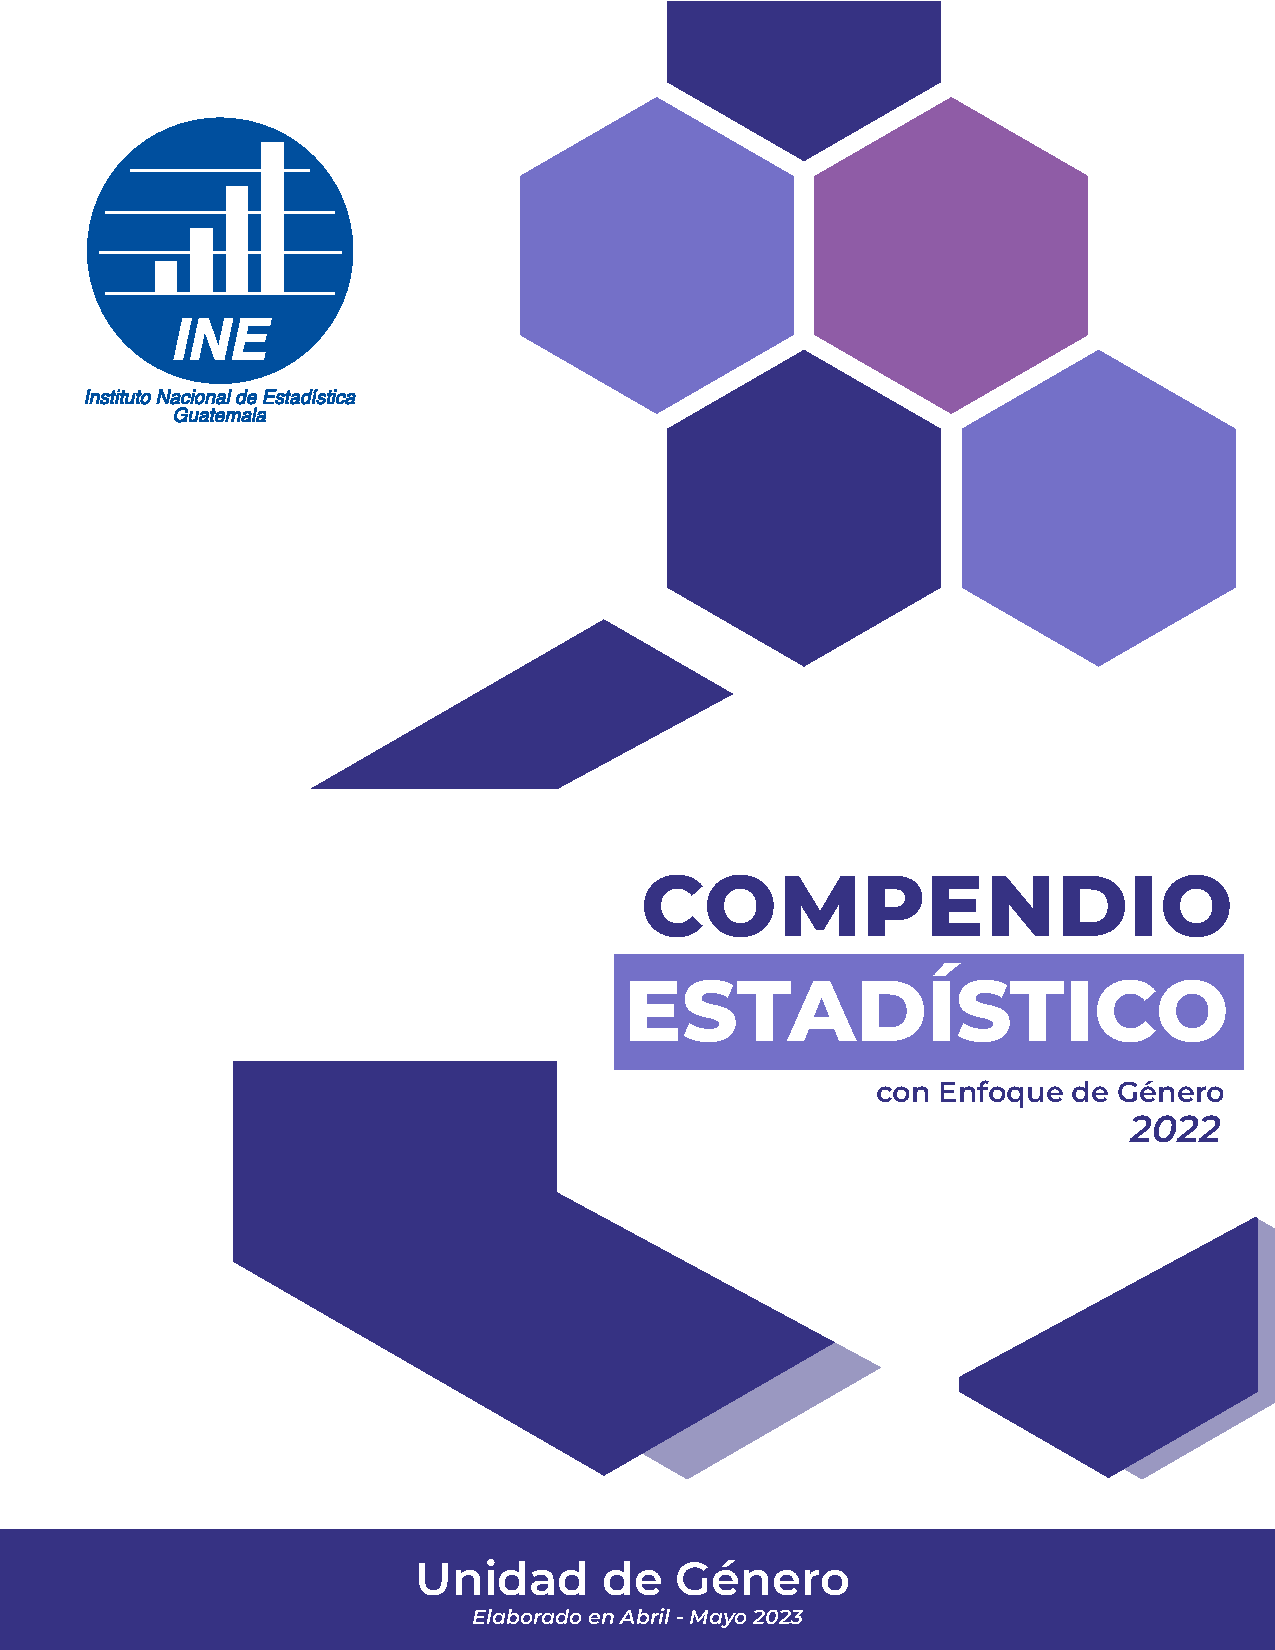
\includepdf{Plantilla/Portada_CEEG_2022.pdf}
	\cleardoublepage
	\thispagestyle{soloarriba}
	\begin{center}
		{\Bold \LARGE AUTORIDADES}\\[1cm]
{\Bold \large \color{color3} JUNTA  DIRECTIVA} \\[0.4cm]
{\Bold Ministerio de Economía}\\ 
Titular: Janio Moacyr Rosales Alegría \\ 
Suplente: Francisca de Jesús Cárdenas Morán\\[0.4cm]

{\Bold Ministerio de Finanzas Públicas}\\ 
Titular: Edwin Oswaldo Martínez Cameros\\ 
Suplente: José Hugo Valle Alegría\\[0.4cm]

{\Bold Ministerio de Agricultura, Ganadería y Alimentación}\\ 
Titular: Edgar René De León Moreno\\ 
Suplente: César Vinicio Arreaga Morales\\[0.4cm]

{\Bold Ministerio de Energía y Minas}\\ 
Titular: Alberto Pimentel Mata\\ 
Suplente: Oscar Rafael Pérez Ramírez\\[0.4cm]

{\Bold Secretaría de Planificación y Programación de la Presidencia}\\ 
Titular: Luz Keila Virginia Gramajo Vilchez\\ 
Suplente: Manuel Augusto Alonzo Araujo\\[0.4cm]

{\Bold Banco de Guatemala}\\ 
Titular: Álvaro González Ricci \\ 
Suplente: José Alfredo Blanco Valdés\\[0.4cm]

{\Bold Universidad de San Carlos de Guatemala}\\ 
Titular: Sindy Massiel Godínez Bautista\\ 
Suplente: José Lara Samayoa\\[0.4cm]

{\Bold Universidades Privadas}\\ 
Titular: Miguel Ángel Franco de León\\ 
Suplente: Oscar Leonel Herrera Velásquez\\[0.4cm]

{\Bold Comité Coordinador de Asociaciones Agrícolas, Comerciales, Industriales y Financieras}\\ 
Titular: Hugo Leonel Maúl Rivas\\ 
Suplente: Ricardo Antonio Rodríguez Martínez\\[0.4cm]

{\Bold \large \color{color3} GERENCIA}\\[0.2cm]
Gerente: Brenda Izabel Miranda Consuegra\\ 
Subgerente Técnico: Hugo Allan García Monterrosa\\ 
Subgerente Administrativo Financiero: Marco Antonio Mejía Villatoro\\ 

	\end{center}
	\cleardoublepage
	$\ $
	\vspace{0.0cm}
	\thispagestyle{soloarriba}
	\begin{center}
		{\Bold \LARGE \color{color3} EQUIPO RESPONSABLE}\\[2cm]
%{\Bold \large \color{color1!89!black} REVISIÓN GENERAL}\\[0.2cm]
%Brenda Izabel Miranda Consuegra\\[0.8cm]
{\Bold \large \color{color2} EQUIPO TÉCNICO}\\[0.2cm]
Brenda Izabel Miranda Consuegra\\
Hugo Allan García Monterrosa\\
Edgar Edwardo Herrarte Rodríguez\\
Julio Roberto Ramírez Pacheco \\
Luis Fernando Castellanos Bonilla \\
María Eugenia Guzmán Chete\\
Cristian Miguel Cabrera Ayala\\
Marvin Isaac Reyes López\\
Patricia Eugenia Hernandez García\\
Paula Natalia Gálvez Molina\\
Rodrigo Rafael Castillo Chong\\
Gerardo Ernesto Rodríguez\\
Mario Raul Soto Gómez\\
Luis Alberto Peñate López\\[0.8cm]
{\Bold \large \color{color2} DIAGRAMACIÓN Y DISEÑO}\\[0.2cm]
Andrea Michelle Rojas Salvatierra\\[0.8cm]

	\end{center}
	\cleardoublepage
	$\ $
	\vspace{0.0cm}
	\thispagestyle{soloarriba}
	$\ $\\[3cm]
\begin{center}
{\Bold \LARGE PRESENTACIÓN}\\[2cm]
\end{center}

El Instituto Nacional de Estadística -INE- tiene por objeto formular y realizar la política estadística nacional, a la vez, tiene como función ser el ente rector central de información, recolección, elaboración y publicación de datos estadísticos oficiales.  

En el cumplimiento de las funciones mencionadas, como Gerente del INE me complace presentar el compendio estadístico con enfoque de género 2022 que tiene como objetivo visibilizar estadísticas y una caracterización en los ámbitos de: demografía, educación, salud, economía, empleo, violencias contra las mujeres y participación sociopolítica, entre otros temas. 

El presente documento es el resultado de un esfuerzo colaborativo de recolección y análisis estadístico entre diversas fuentas de información del INE pertenecientes al Sistema Estadístico Nacional -SEN- que proporcionaron información estratégica que confluye en las derección es y dependencias del INE. A las direcciones y representaciones institucionales agradecemos el compromiso y trabajo realizado. A la vez, se convierte en un aporte al diálogo y análisis sobre situación social, económica y política de las mujeres, como una herramienta útil para las instituciones, organizaciones y personas usuarias que trabajan en la promoción de la igualdad de género para la implementación y promoción de políticas y programas públicos y sociales de desarrollo inclusivo y sostenible en Guatemala.\\[1cm]

\begin{center}
\textbf{Brenda Izabel Miranda Consuegra}\\[0.2cm]
Gerente del Instituto Nacional de Estadística -INE-
\end{center}


	\cleardoublepage
	$\ $\\[2cm]
	\tableofcontents
	\pagestyle{estandar}	
	\vspace{0.0cm}
	\clearpage
	\setcounter{page}{0}
	
%	\INEchaptercarta{Población y demografía}{Capítulo dedicado a mostrar una composición general de las personas que habitan en el territorio guatemalteco respecto a su tamaño y su estructura de la población diferenciada por sexo, por edad, contribuyendo a la construcción de indicadores de la dinámica demográfica, a nivel nacional con un enfoque de género y pueblos.}
%	\cajita{Producto interno bruto}{Para 2022, el grupo de edad de 0 a 4 años tuvo la población más grande de los grupos de edad con 1,870.5 miles de personas. El siguiente grupo más poblado fuel el de 5 a 9 años de edad con 1,864.1 miles de personas. Por el contrario,  la población de 100 años o más contó con la menor cantidad de personas de todos los grupos con 2.8 miles de personas. 

Las estimaciones indican que en los grupos quinquenales desde 0 hasta 24 años, predominaba la población de hombres. Sin embargo, en los grupos quinquenales a partir de los 25 años en adelante, predominaba la población de mujeres. Se estima que para 2022 hubo 277.0 miles de mujeres más que hombres.}{Producto interno bruto}{República de Guatemala, Banco de Guatemala, en millones de quetzales}{\begin{tikzpicture}[x=1pt,y=1pt]% Created by tikzDevice version 0.12.4 on 2023-02-21 13:38:04
% !TEX encoding = UTF-8 Unicode
\definecolor{fillColor}{RGB}{255,255,255}
\path[use as bounding box,fill=fillColor,fill opacity=0.00] (0,0) rectangle (289.08,198.74);
\begin{scope}
\path[clip] (  0.00,  0.00) rectangle (289.08,198.74);

\path[] (  0.00,  0.00) rectangle (289.08,198.74);
\end{scope}
\begin{scope}
\path[clip] (  0.00,  0.00) rectangle (289.08,198.74);
\definecolor{drawColor}{RGB}{51,170,185}

\path[draw=drawColor,line width= 1.7pt,line join=round] ( 38.47, 83.93) --
	( 81.70, 93.46) --
	(124.92,105.02) --
	(168.15, 99.72) --
	(211.38,123.28) --
	(254.61,136.12);
\definecolor{drawColor}{RGB}{0,0,0}

\node[text=drawColor,anchor=base,inner sep=0pt, outer sep=0pt, scale=  1.02] at ( 38.47, 72.02) {479,120.8};

\node[text=drawColor,anchor=base east,inner sep=0pt, outer sep=0pt, scale=  1.02] at ( 74.55, 93.46) {495,443.9};

\node[text=drawColor,anchor=base,inner sep=0pt, outer sep=0pt, scale=  1.02] at (124.92,108.99) {515,273.1};

\node[text=drawColor,anchor=base,inner sep=0pt, outer sep=0pt, scale=  1.02] at (168.15, 87.81) {506,183.2};

\node[text=drawColor,anchor=base east,inner sep=0pt, outer sep=0pt, scale=  1.02] at (204.23,123.28) {546,580.6};

\node[text=drawColor,anchor=base,inner sep=0pt, outer sep=0pt, scale=  1.02] at (254.61,140.09) {568,578.8};

\path[draw=drawColor,line width= 0.1pt,line join=round] (-255.48, 26.12) -- (548.56, 26.12);

\path[] ( 12.53, 18.24) rectangle (280.54,191.48);

\path[] ( 12.53, 66.95) --
	(280.54, 66.95);

\path[] ( 12.53,125.28) --
	(280.54,125.28);

\path[] ( 12.53,183.61) --
	(280.54,183.61);

\path[] ( 12.53, 37.78) --
	(280.54, 37.78);

\path[] ( 12.53, 96.11) --
	(280.54, 96.11);

\path[] ( 12.53,154.44) --
	(280.54,154.44);

\path[] ( 38.47, 18.24) --
	( 38.47,191.48);

\path[] ( 81.70, 18.24) --
	( 81.70,191.48);

\path[] (124.92, 18.24) --
	(124.92,191.48);

\path[] (168.15, 18.24) --
	(168.15,191.48);

\path[] (211.38, 18.24) --
	(211.38,191.48);

\path[] (254.61, 18.24) --
	(254.61,191.48);

\path[] ( 12.53, 18.24) rectangle (280.54,191.48);
\end{scope}
\begin{scope}
\path[clip] (  0.00,  0.00) rectangle (289.08,198.74);

\path[] ( 12.53, 18.24) --
	( 12.53,191.48);
\end{scope}
\begin{scope}
\path[clip] (  0.00,  0.00) rectangle (289.08,198.74);
\definecolor{drawColor}{RGB}{255,255,255}

\node[text=drawColor,text opacity=0.00,anchor=base east,inner sep=0pt, outer sep=0pt, scale=  1.00] at (  7.58, 33.87) {4e+05};

\node[text=drawColor,text opacity=0.00,anchor=base east,inner sep=0pt, outer sep=0pt, scale=  1.00] at (  7.58, 92.20) {5e+05};

\node[text=drawColor,text opacity=0.00,anchor=base east,inner sep=0pt, outer sep=0pt, scale=  1.00] at (  7.58,150.53) {6e+05};
\end{scope}
\begin{scope}
\path[clip] (  0.00,  0.00) rectangle (289.08,198.74);

\path[] (  9.78, 37.78) --
	( 12.53, 37.78);

\path[] (  9.78, 96.11) --
	( 12.53, 96.11);

\path[] (  9.78,154.44) --
	( 12.53,154.44);
\end{scope}
\begin{scope}
\path[clip] (  0.00,  0.00) rectangle (289.08,198.74);

\path[] ( 12.53, 18.24) --
	(280.54, 18.24);
\end{scope}
\begin{scope}
\path[clip] (  0.00,  0.00) rectangle (289.08,198.74);

\path[] ( 38.47, 15.49) --
	( 38.47, 18.24);

\path[] ( 81.70, 15.49) --
	( 81.70, 18.24);

\path[] (124.92, 15.49) --
	(124.92, 18.24);

\path[] (168.15, 15.49) --
	(168.15, 18.24);

\path[] (211.38, 15.49) --
	(211.38, 18.24);

\path[] (254.61, 15.49) --
	(254.61, 18.24);
\end{scope}
\begin{scope}
\path[clip] (  0.00,  0.00) rectangle (289.08,198.74);
\definecolor{drawColor}{RGB}{0,0,0}

\node[text=drawColor,anchor=base,inner sep=0pt, outer sep=0pt, scale=  1.00] at ( 38.47,  4.16) {2017};

\node[text=drawColor,anchor=base,inner sep=0pt, outer sep=0pt, scale=  1.00] at ( 81.70,  4.16) {2018};

\node[text=drawColor,anchor=base,inner sep=0pt, outer sep=0pt, scale=  1.00] at (124.92,  4.16) {2019};

\node[text=drawColor,anchor=base,inner sep=0pt, outer sep=0pt, scale=  1.00] at (168.15,  4.16) {2020};

\node[text=drawColor,anchor=base,inner sep=0pt, outer sep=0pt, scale=  1.00] at (211.38,  4.16) {2021};

\node[text=drawColor,anchor=base,inner sep=0pt, outer sep=0pt, scale=  1.00] at (254.61,  4.16) {2022};
\end{scope}
\end{tikzpicture}}{Banco de Guatemala}{}

\cajita{Proyecciones de Población}{Para 2018, la mayoría de la población se encuentra en el área urbana son mujeres representando el 27.9\%. }{Proyecciones de población}{República de Guatemala, Instituto Nacional de Estadística -INE-, en número de personas}{\begin{tikzpicture}[x=1pt,y=1pt]% Created by tikzDevice version 0.12.4 on 2023-05-05 09:28:13
% !TEX encoding = UTF-8 Unicode
\definecolor{fillColor}{RGB}{255,255,255}
\path[use as bounding box,fill=fillColor,fill opacity=0.00] (0,0) rectangle (289.08,198.74);
\begin{scope}
\path[clip] (  0.00,  0.00) rectangle (289.08,198.74);
\definecolor{drawColor}{RGB}{255,255,255}
\definecolor{fillColor}{RGB}{255,255,255}

\path[draw=drawColor,line width= 0.6pt,line join=round,line cap=round,fill=fillColor] ( 37.81,  0.00) rectangle (251.27,198.74);
\end{scope}
\begin{scope}
\path[clip] (  0.00,  0.00) rectangle (289.08,198.74);
\definecolor{fillColor}{RGB}{54,50,131}

\path[fill=fillColor] (114.85,124.45) --
	(114.85,126.34) --
	(114.85,128.24) --
	(114.85,130.14) --
	(114.85,132.04) --
	(114.85,133.93) --
	(114.85,135.83) --
	(114.85,137.73) --
	(114.85,139.63) --
	(114.85,141.53) --
	(112.94,141.42) --
	(111.06,141.10) --
	(109.22,140.57) --
	(107.45,139.84) --
	(105.77,138.91) --
	(104.21,137.81) --
	(102.78,136.53) --
	(101.51,135.10) --
	(100.40,133.54) --
	( 99.47,131.87) --
	( 98.74,130.10) --
	( 98.20,128.26) --
	( 97.88,126.38) --
	( 97.77,124.47) --
	( 97.88,122.56) --
	( 98.19,120.67) --
	( 98.72,118.83) --
	( 99.45,117.06) --
	(100.37,115.38) --
	(101.48,113.82) --
	(102.75,112.39) --
	(104.18,111.11) --
	(105.74,110.00) --
	(107.41,109.07) --
	(109.17,108.34) --
	(111.01,107.80) --
	(112.90,107.48) --
	(114.81,107.36) --
	(116.72,107.47) --
	(118.61,107.78) --
	(118.19,109.63) --
	(117.77,111.49) --
	(117.36,113.34) --
	(116.94,115.19) --
	(116.52,117.04) --
	(116.10,118.89) --
	(115.69,120.74) --
	(115.27,122.59) --
	(114.85,124.45) --
	(114.85,124.45) --
	cycle;

\path[fill=fillColor] (114.85,143.42) --
	(114.85,145.32) --
	(114.85,147.22) --
	(114.85,149.12) --
	(114.85,151.02) --
	(114.85,152.91) --
	(114.85,154.81) --
	(114.85,156.71) --
	(114.85,158.61) --
	(114.85,160.50) --
	(112.96,160.45) --
	(111.08,160.31) --
	(109.21,160.06) --
	(107.35,159.72) --
	(105.52,159.27) --
	(103.70,158.74) --
	(101.92,158.11) --
	(100.18,157.38) --
	( 98.48,156.57) --
	( 96.82,155.67) --
	( 95.21,154.68) --
	( 93.65,153.61) --
	( 92.15,152.46) --
	( 90.72,151.23) --
	( 89.35,149.93) --
	( 88.05,148.56) --
	( 86.82,147.13) --
	( 85.67,145.63) --
	( 84.60,144.07) --
	( 83.62,142.46) --
	( 82.72,140.80) --
	( 81.90,139.09) --
	( 81.18,137.35) --
	( 80.55,135.57) --
	( 80.02,133.76) --
	( 79.58,131.92) --
	( 79.23,130.06) --
	( 78.99,128.19) --
	( 78.84,126.31) --
	( 78.79,124.42) --
	( 78.84,122.53) --
	( 78.99,120.65) --
	( 79.24,118.77) --
	( 79.59,116.92) --
	( 80.03,115.08) --
	( 80.57,113.27) --
	( 81.20,111.49) --
	( 81.93,109.75) --
	( 82.74,108.04) --
	( 83.64,106.38) --
	( 84.63,104.77) --
	( 85.70,103.22) --
	( 86.85,101.72) --
	( 88.08,100.29) --
	( 89.38, 98.92) --
	( 90.76, 97.62) --
	( 92.19, 96.40) --
	( 93.69, 95.25) --
	( 95.25, 94.18) --
	( 96.86, 93.19) --
	( 98.52, 92.30) --
	(100.23, 91.48) --
	(101.98, 90.76) --
	(103.76, 90.14) --
	(105.57, 89.60) --
	(107.41, 89.16) --
	(109.26, 88.82) --
	(111.14, 88.58) --
	(113.02, 88.43) --
	(114.91, 88.39) --
	(116.80, 88.44) --
	(118.68, 88.59) --
	(120.55, 88.84) --
	(122.41, 89.19) --
	(122.01, 91.04) --
	(121.61, 92.90) --
	(121.21, 94.75) --
	(120.82, 96.61) --
	(120.42, 98.46) --
	(120.02,100.32) --
	(119.62,102.18) --
	(119.23,104.03) --
	(118.83,105.89) --
	(116.98,105.59) --
	(115.12,105.47) --
	(113.25,105.53) --
	(111.39,105.78) --
	(109.57,106.22) --
	(107.80,106.82) --
	(106.10,107.60) --
	(104.49,108.55) --
	(102.97,109.65) --
	(101.57,110.89) --
	(100.30,112.26) --
	( 99.17,113.75) --
	( 98.20,115.35) --
	( 97.38,117.03) --
	( 96.74,118.79) --
	( 96.27,120.60) --
	( 95.98,122.45) --
	( 95.87,124.31) --
	( 95.95,126.18) --
	( 96.22,128.03) --
	( 96.66,129.85) --
	( 97.28,131.62) --
	( 98.07,133.31) --
	( 99.03,134.92) --
	(100.14,136.43) --
	(101.39,137.82) --
	(102.77,139.08) --
	(104.27,140.20) --
	(105.87,141.16) --
	(107.56,141.97) --
	(109.32,142.60) --
	(111.13,143.06) --
	(112.98,143.33) --
	(114.85,143.42) --
	cycle;

\path[fill=fillColor] (114.85,162.40) --
	(114.85,164.30) --
	(114.85,166.20) --
	(114.85,168.10) --
	(114.85,169.99) --
	(114.85,171.89) --
	(114.85,173.79) --
	(114.85,175.69) --
	(114.85,177.59) --
	(114.85,179.48) --
	(112.99,179.45) --
	(111.13,179.36) --
	(109.27,179.20) --
	(107.42,178.98) --
	(105.58,178.70) --
	(103.75,178.35) --
	(101.93,177.94) --
	(100.13,177.48) --
	( 98.34,176.95) --
	( 96.57,176.36) --
	( 94.83,175.71) --
	( 93.10,175.00) --
	( 91.41,174.24) --
	( 89.73,173.42) --
	( 88.09,172.54) --
	( 86.48,171.60) --
	( 84.90,170.62) --
	( 83.35,169.58) --
	( 81.84,168.48) --
	( 80.37,167.34) --
	( 78.94,166.15) --
	( 77.55,164.91) --
	( 76.20,163.63) --
	( 74.90,162.29) --
	( 73.64,160.92) --
	( 72.43,159.50) --
	( 71.26,158.05) --
	( 70.15,156.55) --
	( 69.09,155.02) --
	( 68.08,153.46) --
	( 67.13,151.86) --
	( 66.23,150.22) --
	( 65.38,148.56) --
	( 64.59,146.88) --
	( 63.86,145.16) --
	( 63.19,143.42) --
	( 62.58,141.66) --
	( 62.03,139.89) --
	( 61.53,138.09) --
	( 61.10,136.28) --
	( 60.73,134.45) --
	( 60.42,132.61) --
	( 60.18,130.77) --
	( 60.00,128.91) --
	( 59.88,127.05) --
	( 59.82,125.19) --
	( 59.83,123.33) --
	( 59.90,121.46) --
	( 60.03,119.61) --
	( 60.22,117.75) --
	( 60.48,115.91) --
	( 60.80,114.07) --
	( 61.18,112.25) --
	( 61.63,110.44) --
	( 62.13,108.65) --
	( 62.70,106.87) --
	( 63.32,105.11) --
	( 64.01,103.38) --
	( 64.75,101.67) --
	( 65.55, 99.99) --
	( 66.40, 98.33) --
	( 67.31, 96.71) --
	( 68.28, 95.12) --
	( 69.30, 93.56) --
	( 70.37, 92.03) --
	( 71.49, 90.55) --
	( 72.67, 89.10) --
	( 73.89, 87.69) --
	( 75.15, 86.32) --
	( 76.47, 85.00) --
	( 77.82, 83.73) --
	( 79.22, 82.50) --
	( 80.66, 81.31) --
	( 82.14, 80.18) --
	( 83.66, 79.10) --
	( 85.21, 78.07) --
	( 86.80, 77.09) --
	( 88.42, 76.17) --
	( 90.07, 75.30) --
	( 91.74, 74.49) --
	( 93.45, 73.74) --
	( 95.18, 73.04) --
	( 96.93, 72.41) --
	( 98.70, 71.83) --
	(100.49, 71.31) --
	(102.30, 70.86) --
	(104.12, 70.46) --
	(105.95, 70.13) --
	(107.79, 69.86) --
	(109.65, 69.65) --
	(111.50, 69.51) --
	(113.36, 69.43) --
	(115.23, 69.41) --
	(117.09, 69.45) --
	(118.95, 69.56) --
	(120.81, 69.73) --
	(122.65, 69.96) --
	(124.49, 70.26) --
	(124.16, 72.13) --
	(123.83, 74.00) --
	(123.50, 75.86) --
	(123.16, 77.73) --
	(122.83, 79.60) --
	(122.50, 81.47) --
	(122.17, 83.34) --
	(121.83, 85.21) --
	(121.50, 87.07) --
	(119.64, 86.79) --
	(117.77, 86.60) --
	(115.90, 86.50) --
	(114.02, 86.50) --
	(112.14, 86.58) --
	(110.27, 86.77) --
	(108.41, 87.04) --
	(106.57, 87.40) --
	(104.74, 87.86) --
	(102.95, 88.40) --
	(101.18, 89.04) --
	( 99.44, 89.76) --
	( 97.74, 90.56) --
	( 96.09, 91.45) --
	( 94.48, 92.42) --
	( 92.92, 93.47) --
	( 91.41, 94.59) --
	( 89.96, 95.79) --
	( 88.57, 97.06) --
	( 87.25, 98.39) --
	( 85.99, 99.79) --
	( 84.81,101.25) --
	( 83.70,102.76) --
	( 82.66,104.33) --
	( 81.71,105.95) --
	( 80.83,107.61) --
	( 80.04,109.32) --
	( 79.33,111.06) --
	( 78.72,112.83) --
	( 78.18,114.64) --
	( 77.74,116.46) --
	( 77.39,118.31) --
	( 77.14,120.17) --
	( 76.97,122.04) --
	( 76.90,123.92) --
	( 76.92,125.80) --
	( 77.03,127.68) --
	( 77.24,129.55) --
	( 77.54,131.40) --
	( 77.93,133.24) --
	( 78.41,135.06) --
	( 78.98,136.85) --
	( 79.64,138.61) --
	( 80.38,140.33) --
	( 81.21,142.02) --
	( 82.12,143.66) --
	( 83.11,145.26) --
	( 84.18,146.81) --
	( 85.33,148.30) --
	( 86.54,149.73) --
	( 87.83,151.10) --
	( 89.18,152.40) --
	( 90.60,153.64) --
	( 92.07,154.81) --
	( 93.60,155.90) --
	( 95.19,156.91) --
	( 96.82,157.84) --
	( 98.49,158.69) --
	(100.21,159.46) --
	(101.96,160.14) --
	(103.74,160.74) --
	(105.55,161.24) --
	(107.38,161.66) --
	(109.23,161.98) --
	(111.10,162.22) --
	(112.97,162.36) --
	(114.85,162.40) --
	cycle;
\definecolor{fillColor}{RGB}{116,112,200}

\path[fill=fillColor] (114.85,124.45) --
	(115.27,122.59) --
	(115.69,120.74) --
	(116.10,118.89) --
	(116.52,117.04) --
	(116.94,115.19) --
	(117.36,113.34) --
	(117.77,111.49) --
	(118.19,109.63) --
	(118.61,107.78) --
	(120.45,108.31) --
	(122.23,109.04) --
	(123.91,109.96) --
	(125.47,111.07) --
	(126.90,112.34) --
	(128.18,113.77) --
	(129.30,115.33) --
	(130.23,117.01) --
	(130.97,118.77) --
	(131.50,120.62) --
	(131.82,122.51) --
	(131.93,124.42) --
	(131.83,126.33) --
	(131.51,128.22) --
	(130.98,130.07) --
	(130.25,131.84) --
	(129.32,133.52) --
	(128.22,135.08) --
	(126.94,136.51) --
	(125.51,137.79) --
	(123.95,138.90) --
	(122.27,139.83) --
	(120.50,140.57) --
	(118.66,141.10) --
	(116.77,141.42) --
	(114.85,141.53) --
	(114.85,139.63) --
	(114.85,137.73) --
	(114.85,135.83) --
	(114.85,133.93) --
	(114.85,132.04) --
	(114.85,130.14) --
	(114.85,128.24) --
	(114.85,126.34) --
	(114.85,124.45) --
	(114.85,124.45) --
	cycle;

\path[fill=fillColor] (118.83,105.89) --
	(119.23,104.03) --
	(119.62,102.18) --
	(120.02,100.32) --
	(120.42, 98.46) --
	(120.82, 96.61) --
	(121.21, 94.75) --
	(121.61, 92.90) --
	(122.01, 91.04) --
	(122.41, 89.19) --
	(124.24, 89.63) --
	(126.05, 90.17) --
	(127.83, 90.80) --
	(129.57, 91.53) --
	(131.27, 92.34) --
	(132.93, 93.24) --
	(134.53, 94.23) --
	(136.09, 95.30) --
	(137.58, 96.45) --
	(139.02, 97.68) --
	(140.38, 98.98) --
	(141.68,100.35) --
	(142.90,101.79) --
	(144.05,103.29) --
	(145.12,104.84) --
	(146.10,106.45) --
	(147.00,108.11) --
	(147.81,109.81) --
	(148.53,111.56) --
	(149.16,113.34) --
	(149.69,115.15) --
	(150.13,116.98) --
	(150.47,118.84) --
	(150.72,120.71) --
	(150.86,122.59) --
	(150.91,124.48) --
	(150.86,126.36) --
	(150.71,128.24) --
	(150.46,130.11) --
	(150.12,131.97) --
	(149.68,133.80) --
	(149.14,135.61) --
	(148.51,137.39) --
	(147.79,139.13) --
	(146.97,140.84) --
	(146.07,142.49) --
	(145.08,144.10) --
	(144.01,145.66) --
	(142.87,147.15) --
	(141.64,148.59) --
	(140.34,149.95) --
	(138.97,151.25) --
	(137.54,152.48) --
	(136.04,153.62) --
	(134.48,154.69) --
	(132.87,155.68) --
	(131.22,156.58) --
	(129.51,157.39) --
	(127.77,158.11) --
	(125.99,158.74) --
	(124.18,159.28) --
	(122.35,159.72) --
	(120.49,160.06) --
	(118.62,160.31) --
	(116.74,160.46) --
	(114.85,160.50) --
	(114.85,158.61) --
	(114.85,156.71) --
	(114.85,154.81) --
	(114.85,152.91) --
	(114.85,151.02) --
	(114.85,149.12) --
	(114.85,147.22) --
	(114.85,145.32) --
	(114.85,143.42) --
	(116.77,143.33) --
	(118.66,143.04) --
	(120.52,142.56) --
	(122.32,141.89) --
	(124.04,141.05) --
	(125.67,140.04) --
	(127.19,138.87) --
	(128.58,137.55) --
	(129.83,136.10) --
	(130.93,134.53) --
	(131.87,132.86) --
	(132.63,131.10) --
	(133.21,129.27) --
	(133.60,127.39) --
	(133.80,125.49) --
	(133.81,123.57) --
	(133.63,121.66) --
	(133.25,119.78) --
	(132.69,117.95) --
	(131.94,116.19) --
	(131.02,114.50) --
	(129.93,112.92) --
	(128.69,111.46) --
	(127.31,110.13) --
	(125.81,108.95) --
	(124.19,107.92) --
	(122.47,107.06) --
	(120.68,106.38) --
	(118.83,105.89) --
	cycle;

\path[fill=fillColor] (121.50, 87.07) --
	(121.83, 85.21) --
	(122.17, 83.34) --
	(122.50, 81.47) --
	(122.83, 79.60) --
	(123.16, 77.73) --
	(123.50, 75.86) --
	(123.83, 74.00) --
	(124.16, 72.13) --
	(124.49, 70.26) --
	(126.34, 70.62) --
	(128.16, 71.04) --
	(129.98, 71.53) --
	(131.77, 72.07) --
	(133.54, 72.68) --
	(135.30, 73.35) --
	(137.03, 74.07) --
	(138.73, 74.86) --
	(140.41, 75.70) --
	(142.05, 76.60) --
	(143.67, 77.55) --
	(145.25, 78.56) --
	(146.80, 79.63) --
	(148.31, 80.74) --
	(149.78, 81.91) --
	(151.20, 83.12) --
	(152.59, 84.38) --
	(153.94, 85.69) --
	(155.23, 87.05) --
	(156.48, 88.44) --
	(157.69, 89.88) --
	(158.84, 91.36) --
	(159.94, 92.88) --
	(160.99, 94.44) --
	(161.99, 96.03) --
	(162.93, 97.65) --
	(163.81, 99.30) --
	(164.64,100.99) --
	(165.41,102.70) --
	(166.12,104.43) --
	(166.78,106.19) --
	(167.37,107.97) --
	(167.90,109.77) --
	(168.37,111.59) --
	(168.78,113.42) --
	(169.12,115.26) --
	(169.40,117.12) --
	(169.62,118.98) --
	(169.77,120.85) --
	(169.86,122.72) --
	(169.89,124.60) --
	(169.85,126.48) --
	(169.75,128.35) --
	(169.59,130.22) --
	(169.36,132.08) --
	(169.07,133.93) --
	(168.71,135.78) --
	(168.29,137.60) --
	(167.82,139.42) --
	(167.27,141.21) --
	(166.67,142.99) --
	(166.01,144.75) --
	(165.29,146.48) --
	(164.51,148.18) --
	(163.67,149.86) --
	(162.78,151.51) --
	(161.83,153.13) --
	(160.82,154.71) --
	(159.76,156.26) --
	(158.65,157.77) --
	(157.49,159.25) --
	(156.28,160.68) --
	(155.02,162.07) --
	(153.72,163.42) --
	(152.36,164.72) --
	(150.97,165.97) --
	(149.53,167.18) --
	(148.06,168.34) --
	(146.54,169.44) --
	(144.99,170.50) --
	(143.40,171.50) --
	(141.78,172.44) --
	(140.13,173.33) --
	(138.45,174.17) --
	(136.74,174.94) --
	(135.01,175.66) --
	(133.25,176.32) --
	(131.47,176.91) --
	(129.68,177.45) --
	(127.86,177.92) --
	(126.03,178.34) --
	(124.19,178.69) --
	(122.33,178.97) --
	(120.47,179.20) --
	(118.60,179.36) --
	(116.73,179.45) --
	(114.85,179.48) --
	(114.85,177.59) --
	(114.85,175.69) --
	(114.85,173.79) --
	(114.85,171.89) --
	(114.85,169.99) --
	(114.85,168.10) --
	(114.85,166.20) --
	(114.85,164.30) --
	(114.85,162.40) --
	(116.73,162.36) --
	(118.60,162.22) --
	(120.46,161.99) --
	(122.31,161.66) --
	(124.14,161.25) --
	(125.94,160.75) --
	(127.72,160.15) --
	(129.47,159.47) --
	(131.19,158.71) --
	(132.86,157.86) --
	(134.49,156.93) --
	(136.07,155.92) --
	(137.60,154.83) --
	(139.07,153.67) --
	(140.49,152.44) --
	(141.84,151.14) --
	(143.12,149.77) --
	(144.34,148.35) --
	(145.48,146.86) --
	(146.55,145.32) --
	(147.55,143.73) --
	(148.46,142.09) --
	(149.29,140.41) --
	(150.04,138.69) --
	(150.70,136.93) --
	(151.27,135.14) --
	(151.76,133.33) --
	(152.15,131.50) --
	(152.45,129.65) --
	(152.66,127.78) --
	(152.78,125.91) --
	(152.81,124.03) --
	(152.74,122.16) --
	(152.58,120.29) --
	(152.33,118.43) --
	(151.99,116.59) --
	(151.55,114.76) --
	(151.03,112.96) --
	(150.42,111.19) --
	(149.72,109.45) --
	(148.94,107.74) --
	(148.07,106.08) --
	(147.12,104.46) --
	(146.10,102.89) --
	(144.99,101.37) --
	(143.82, 99.91) --
	(142.57, 98.51) --
	(141.25, 97.17) --
	(139.87, 95.90) --
	(138.43, 94.70) --
	(136.94, 93.57) --
	(135.38, 92.52) --
	(133.78, 91.54) --
	(132.13, 90.65) --
	(130.44, 89.84) --
	(128.71, 89.11) --
	(126.95, 88.47) --
	(125.16, 87.91) --
	(123.34, 87.45) --
	(121.50, 87.07) --
	cycle;
\definecolor{drawColor}{RGB}{255,255,255}

\node[text=drawColor,anchor=base,inner sep=0pt, outer sep=0pt, scale=  0.78] at (106.36,120.47) {9.2};

\node[text=drawColor,anchor=base,inner sep=0pt, outer sep=0pt, scale=  0.78] at ( 87.49,118.51) {12.8};

\node[text=drawColor,anchor=base,inner sep=0pt, outer sep=0pt, scale=  0.78] at ( 68.54,117.32) {31.1};

\node[text=drawColor,anchor=base,inner sep=0pt, outer sep=0pt, scale=  0.78] at (123.34,122.36) {8.0};

\node[text=drawColor,anchor=base,inner sep=0pt, outer sep=0pt, scale=  0.78] at (142.22,124.31) {11.2};

\node[text=drawColor,anchor=base,inner sep=0pt, outer sep=0pt, scale=  0.78] at (161.17,125.50) {27.8};

\node[text=drawColor,anchor=base,inner sep=0pt, outer sep=0pt, scale=  1.03] at (114.85,128.94) {\bfseries 1};

\node[text=drawColor,anchor=base,inner sep=0pt, outer sep=0pt, scale=  1.03] at (114.85,147.92) {\bfseries 2};

\node[text=drawColor,anchor=base,inner sep=0pt, outer sep=0pt, scale=  1.03] at (114.85,166.90) {\bfseries 3};
\end{scope}
\begin{scope}
\path[clip] (  0.00,  0.00) rectangle (289.08,198.74);
\definecolor{fillColor}{RGB}{255,255,255}

\path[fill=fillColor] (194.65, 99.59) rectangle (245.77,149.30);
\end{scope}
\begin{scope}
\path[clip] (  0.00,  0.00) rectangle (289.08,198.74);
\definecolor{fillColor}{gray}{0.95}

\path[fill=fillColor] (200.15,116.47) rectangle (211.53,127.85);
\end{scope}
\begin{scope}
\path[clip] (  0.00,  0.00) rectangle (289.08,198.74);
\definecolor{fillColor}{RGB}{54,50,131}

\path[fill=fillColor] (200.81,117.13) rectangle (210.87,127.19);
\end{scope}
\begin{scope}
\path[clip] (  0.00,  0.00) rectangle (289.08,198.74);
\definecolor{fillColor}{gray}{0.95}

\path[fill=fillColor] (200.15,105.09) rectangle (211.53,116.47);
\end{scope}
\begin{scope}
\path[clip] (  0.00,  0.00) rectangle (289.08,198.74);
\definecolor{fillColor}{RGB}{116,112,200}

\path[fill=fillColor] (200.81,105.75) rectangle (210.87,115.81);
\end{scope}
\begin{scope}
\path[clip] (  0.00,  0.00) rectangle (289.08,198.74);
\definecolor{drawColor}{RGB}{0,0,0}

\node[text=drawColor,anchor=base west,inner sep=0pt, outer sep=0pt, scale=  0.80] at (217.03,119.04) {Mujeres};
\end{scope}
\begin{scope}
\path[clip] (  0.00,  0.00) rectangle (289.08,198.74);
\definecolor{drawColor}{RGB}{0,0,0}

\node[text=drawColor,anchor=base west,inner sep=0pt, outer sep=0pt, scale=  0.80] at (217.03,107.65) {Hombres};
\end{scope}
\begin{scope}
\path[clip] (  0.00,  0.00) rectangle (289.08,198.74);
\definecolor{drawColor}{RGB}{0,0,0}

\node[text=drawColor,anchor=base west,inner sep=0pt, outer sep=0pt, scale=  0.91] at ( 46.06, 40.29) {1: Urbano Metropolitano};

\node[text=drawColor,anchor=base west,inner sep=0pt, outer sep=0pt, scale=  0.91] at ( 46.06, 29.49) {2: Resto Urbano};

\node[text=drawColor,anchor=base west,inner sep=0pt, outer sep=0pt, scale=  0.91] at ( 46.06, 18.69) {3: Rural Nacional};

\node[text=drawColor,anchor=base west,inner sep=0pt, outer sep=0pt, scale=  0.91] at ( 46.06,  7.89) {};
\end{scope}
\end{tikzpicture}}{INE}{}

\cajita{Producto interno bruto}{Para 2022, el grupo de edad de 0 a 4 años tuvo la población más grande de los grupos de edad con 1,870.5 miles de personas. El siguiente grupo más poblado fuel el de 5 a 9 años de edad con 1,864.1 miles de personas. Por el contrario,  la población de 100 años o más contó con la menor cantidad de personas de todos los grupos con 2.8 miles de personas. 

Las estimaciones indican que en los grupos quinquenales desde 0 hasta 24 años, predominaba la población de hombres. Sin embargo, en los grupos quinquenales a partir de los 25 años en adelante, predominaba la población de mujeres. Se estima que para 2022 hubo 277.0 miles de mujeres más que hombres.}{Producto interno bruto}{República de Guatemala, Banco de Guatemala, en millones de quetzales}{\begin{tikzpicture}[x=1pt,y=1pt]% Created by tikzDevice version 0.12.4 on 2023-02-21 13:38:04
% !TEX encoding = UTF-8 Unicode
\definecolor{fillColor}{RGB}{255,255,255}
\path[use as bounding box,fill=fillColor,fill opacity=0.00] (0,0) rectangle (289.08,198.74);
\begin{scope}
\path[clip] (  0.00,  0.00) rectangle (289.08,198.74);

\path[] (  0.00,  0.00) rectangle (289.08,198.74);
\end{scope}
\begin{scope}
\path[clip] (  0.00,  0.00) rectangle (289.08,198.74);
\definecolor{drawColor}{RGB}{51,170,185}

\path[draw=drawColor,line width= 1.7pt,line join=round] ( 38.47, 83.93) --
	( 81.70, 93.46) --
	(124.92,105.02) --
	(168.15, 99.72) --
	(211.38,123.28) --
	(254.61,136.12);
\definecolor{drawColor}{RGB}{0,0,0}

\node[text=drawColor,anchor=base,inner sep=0pt, outer sep=0pt, scale=  1.02] at ( 38.47, 72.02) {479,120.8};

\node[text=drawColor,anchor=base east,inner sep=0pt, outer sep=0pt, scale=  1.02] at ( 74.55, 93.46) {495,443.9};

\node[text=drawColor,anchor=base,inner sep=0pt, outer sep=0pt, scale=  1.02] at (124.92,108.99) {515,273.1};

\node[text=drawColor,anchor=base,inner sep=0pt, outer sep=0pt, scale=  1.02] at (168.15, 87.81) {506,183.2};

\node[text=drawColor,anchor=base east,inner sep=0pt, outer sep=0pt, scale=  1.02] at (204.23,123.28) {546,580.6};

\node[text=drawColor,anchor=base,inner sep=0pt, outer sep=0pt, scale=  1.02] at (254.61,140.09) {568,578.8};

\path[draw=drawColor,line width= 0.1pt,line join=round] (-255.48, 26.12) -- (548.56, 26.12);

\path[] ( 12.53, 18.24) rectangle (280.54,191.48);

\path[] ( 12.53, 66.95) --
	(280.54, 66.95);

\path[] ( 12.53,125.28) --
	(280.54,125.28);

\path[] ( 12.53,183.61) --
	(280.54,183.61);

\path[] ( 12.53, 37.78) --
	(280.54, 37.78);

\path[] ( 12.53, 96.11) --
	(280.54, 96.11);

\path[] ( 12.53,154.44) --
	(280.54,154.44);

\path[] ( 38.47, 18.24) --
	( 38.47,191.48);

\path[] ( 81.70, 18.24) --
	( 81.70,191.48);

\path[] (124.92, 18.24) --
	(124.92,191.48);

\path[] (168.15, 18.24) --
	(168.15,191.48);

\path[] (211.38, 18.24) --
	(211.38,191.48);

\path[] (254.61, 18.24) --
	(254.61,191.48);

\path[] ( 12.53, 18.24) rectangle (280.54,191.48);
\end{scope}
\begin{scope}
\path[clip] (  0.00,  0.00) rectangle (289.08,198.74);

\path[] ( 12.53, 18.24) --
	( 12.53,191.48);
\end{scope}
\begin{scope}
\path[clip] (  0.00,  0.00) rectangle (289.08,198.74);
\definecolor{drawColor}{RGB}{255,255,255}

\node[text=drawColor,text opacity=0.00,anchor=base east,inner sep=0pt, outer sep=0pt, scale=  1.00] at (  7.58, 33.87) {4e+05};

\node[text=drawColor,text opacity=0.00,anchor=base east,inner sep=0pt, outer sep=0pt, scale=  1.00] at (  7.58, 92.20) {5e+05};

\node[text=drawColor,text opacity=0.00,anchor=base east,inner sep=0pt, outer sep=0pt, scale=  1.00] at (  7.58,150.53) {6e+05};
\end{scope}
\begin{scope}
\path[clip] (  0.00,  0.00) rectangle (289.08,198.74);

\path[] (  9.78, 37.78) --
	( 12.53, 37.78);

\path[] (  9.78, 96.11) --
	( 12.53, 96.11);

\path[] (  9.78,154.44) --
	( 12.53,154.44);
\end{scope}
\begin{scope}
\path[clip] (  0.00,  0.00) rectangle (289.08,198.74);

\path[] ( 12.53, 18.24) --
	(280.54, 18.24);
\end{scope}
\begin{scope}
\path[clip] (  0.00,  0.00) rectangle (289.08,198.74);

\path[] ( 38.47, 15.49) --
	( 38.47, 18.24);

\path[] ( 81.70, 15.49) --
	( 81.70, 18.24);

\path[] (124.92, 15.49) --
	(124.92, 18.24);

\path[] (168.15, 15.49) --
	(168.15, 18.24);

\path[] (211.38, 15.49) --
	(211.38, 18.24);

\path[] (254.61, 15.49) --
	(254.61, 18.24);
\end{scope}
\begin{scope}
\path[clip] (  0.00,  0.00) rectangle (289.08,198.74);
\definecolor{drawColor}{RGB}{0,0,0}

\node[text=drawColor,anchor=base,inner sep=0pt, outer sep=0pt, scale=  1.00] at ( 38.47,  4.16) {2017};

\node[text=drawColor,anchor=base,inner sep=0pt, outer sep=0pt, scale=  1.00] at ( 81.70,  4.16) {2018};

\node[text=drawColor,anchor=base,inner sep=0pt, outer sep=0pt, scale=  1.00] at (124.92,  4.16) {2019};

\node[text=drawColor,anchor=base,inner sep=0pt, outer sep=0pt, scale=  1.00] at (168.15,  4.16) {2020};

\node[text=drawColor,anchor=base,inner sep=0pt, outer sep=0pt, scale=  1.00] at (211.38,  4.16) {2021};

\node[text=drawColor,anchor=base,inner sep=0pt, outer sep=0pt, scale=  1.00] at (254.61,  4.16) {2022};
\end{scope}
\end{tikzpicture}}{Banco de Guatemala}{}

\cajita{Proyecciones de Población}{Para 2018, la mayoría de la población se encuentra en el área urbana son mujeres representando el 27.9\%. }{Proyecciones de población}{República de Guatemala, Instituto Nacional de Estadística -INE-, en número de personas}{\begin{tikzpicture}[x=1pt,y=1pt]% Created by tikzDevice version 0.12.4 on 2023-05-05 09:28:13
% !TEX encoding = UTF-8 Unicode
\definecolor{fillColor}{RGB}{255,255,255}
\path[use as bounding box,fill=fillColor,fill opacity=0.00] (0,0) rectangle (289.08,198.74);
\begin{scope}
\path[clip] (  0.00,  0.00) rectangle (289.08,198.74);
\definecolor{drawColor}{RGB}{255,255,255}
\definecolor{fillColor}{RGB}{255,255,255}

\path[draw=drawColor,line width= 0.6pt,line join=round,line cap=round,fill=fillColor] ( 37.81,  0.00) rectangle (251.27,198.74);
\end{scope}
\begin{scope}
\path[clip] (  0.00,  0.00) rectangle (289.08,198.74);
\definecolor{fillColor}{RGB}{54,50,131}

\path[fill=fillColor] (114.85,124.45) --
	(114.85,126.34) --
	(114.85,128.24) --
	(114.85,130.14) --
	(114.85,132.04) --
	(114.85,133.93) --
	(114.85,135.83) --
	(114.85,137.73) --
	(114.85,139.63) --
	(114.85,141.53) --
	(112.94,141.42) --
	(111.06,141.10) --
	(109.22,140.57) --
	(107.45,139.84) --
	(105.77,138.91) --
	(104.21,137.81) --
	(102.78,136.53) --
	(101.51,135.10) --
	(100.40,133.54) --
	( 99.47,131.87) --
	( 98.74,130.10) --
	( 98.20,128.26) --
	( 97.88,126.38) --
	( 97.77,124.47) --
	( 97.88,122.56) --
	( 98.19,120.67) --
	( 98.72,118.83) --
	( 99.45,117.06) --
	(100.37,115.38) --
	(101.48,113.82) --
	(102.75,112.39) --
	(104.18,111.11) --
	(105.74,110.00) --
	(107.41,109.07) --
	(109.17,108.34) --
	(111.01,107.80) --
	(112.90,107.48) --
	(114.81,107.36) --
	(116.72,107.47) --
	(118.61,107.78) --
	(118.19,109.63) --
	(117.77,111.49) --
	(117.36,113.34) --
	(116.94,115.19) --
	(116.52,117.04) --
	(116.10,118.89) --
	(115.69,120.74) --
	(115.27,122.59) --
	(114.85,124.45) --
	(114.85,124.45) --
	cycle;

\path[fill=fillColor] (114.85,143.42) --
	(114.85,145.32) --
	(114.85,147.22) --
	(114.85,149.12) --
	(114.85,151.02) --
	(114.85,152.91) --
	(114.85,154.81) --
	(114.85,156.71) --
	(114.85,158.61) --
	(114.85,160.50) --
	(112.96,160.45) --
	(111.08,160.31) --
	(109.21,160.06) --
	(107.35,159.72) --
	(105.52,159.27) --
	(103.70,158.74) --
	(101.92,158.11) --
	(100.18,157.38) --
	( 98.48,156.57) --
	( 96.82,155.67) --
	( 95.21,154.68) --
	( 93.65,153.61) --
	( 92.15,152.46) --
	( 90.72,151.23) --
	( 89.35,149.93) --
	( 88.05,148.56) --
	( 86.82,147.13) --
	( 85.67,145.63) --
	( 84.60,144.07) --
	( 83.62,142.46) --
	( 82.72,140.80) --
	( 81.90,139.09) --
	( 81.18,137.35) --
	( 80.55,135.57) --
	( 80.02,133.76) --
	( 79.58,131.92) --
	( 79.23,130.06) --
	( 78.99,128.19) --
	( 78.84,126.31) --
	( 78.79,124.42) --
	( 78.84,122.53) --
	( 78.99,120.65) --
	( 79.24,118.77) --
	( 79.59,116.92) --
	( 80.03,115.08) --
	( 80.57,113.27) --
	( 81.20,111.49) --
	( 81.93,109.75) --
	( 82.74,108.04) --
	( 83.64,106.38) --
	( 84.63,104.77) --
	( 85.70,103.22) --
	( 86.85,101.72) --
	( 88.08,100.29) --
	( 89.38, 98.92) --
	( 90.76, 97.62) --
	( 92.19, 96.40) --
	( 93.69, 95.25) --
	( 95.25, 94.18) --
	( 96.86, 93.19) --
	( 98.52, 92.30) --
	(100.23, 91.48) --
	(101.98, 90.76) --
	(103.76, 90.14) --
	(105.57, 89.60) --
	(107.41, 89.16) --
	(109.26, 88.82) --
	(111.14, 88.58) --
	(113.02, 88.43) --
	(114.91, 88.39) --
	(116.80, 88.44) --
	(118.68, 88.59) --
	(120.55, 88.84) --
	(122.41, 89.19) --
	(122.01, 91.04) --
	(121.61, 92.90) --
	(121.21, 94.75) --
	(120.82, 96.61) --
	(120.42, 98.46) --
	(120.02,100.32) --
	(119.62,102.18) --
	(119.23,104.03) --
	(118.83,105.89) --
	(116.98,105.59) --
	(115.12,105.47) --
	(113.25,105.53) --
	(111.39,105.78) --
	(109.57,106.22) --
	(107.80,106.82) --
	(106.10,107.60) --
	(104.49,108.55) --
	(102.97,109.65) --
	(101.57,110.89) --
	(100.30,112.26) --
	( 99.17,113.75) --
	( 98.20,115.35) --
	( 97.38,117.03) --
	( 96.74,118.79) --
	( 96.27,120.60) --
	( 95.98,122.45) --
	( 95.87,124.31) --
	( 95.95,126.18) --
	( 96.22,128.03) --
	( 96.66,129.85) --
	( 97.28,131.62) --
	( 98.07,133.31) --
	( 99.03,134.92) --
	(100.14,136.43) --
	(101.39,137.82) --
	(102.77,139.08) --
	(104.27,140.20) --
	(105.87,141.16) --
	(107.56,141.97) --
	(109.32,142.60) --
	(111.13,143.06) --
	(112.98,143.33) --
	(114.85,143.42) --
	cycle;

\path[fill=fillColor] (114.85,162.40) --
	(114.85,164.30) --
	(114.85,166.20) --
	(114.85,168.10) --
	(114.85,169.99) --
	(114.85,171.89) --
	(114.85,173.79) --
	(114.85,175.69) --
	(114.85,177.59) --
	(114.85,179.48) --
	(112.99,179.45) --
	(111.13,179.36) --
	(109.27,179.20) --
	(107.42,178.98) --
	(105.58,178.70) --
	(103.75,178.35) --
	(101.93,177.94) --
	(100.13,177.48) --
	( 98.34,176.95) --
	( 96.57,176.36) --
	( 94.83,175.71) --
	( 93.10,175.00) --
	( 91.41,174.24) --
	( 89.73,173.42) --
	( 88.09,172.54) --
	( 86.48,171.60) --
	( 84.90,170.62) --
	( 83.35,169.58) --
	( 81.84,168.48) --
	( 80.37,167.34) --
	( 78.94,166.15) --
	( 77.55,164.91) --
	( 76.20,163.63) --
	( 74.90,162.29) --
	( 73.64,160.92) --
	( 72.43,159.50) --
	( 71.26,158.05) --
	( 70.15,156.55) --
	( 69.09,155.02) --
	( 68.08,153.46) --
	( 67.13,151.86) --
	( 66.23,150.22) --
	( 65.38,148.56) --
	( 64.59,146.88) --
	( 63.86,145.16) --
	( 63.19,143.42) --
	( 62.58,141.66) --
	( 62.03,139.89) --
	( 61.53,138.09) --
	( 61.10,136.28) --
	( 60.73,134.45) --
	( 60.42,132.61) --
	( 60.18,130.77) --
	( 60.00,128.91) --
	( 59.88,127.05) --
	( 59.82,125.19) --
	( 59.83,123.33) --
	( 59.90,121.46) --
	( 60.03,119.61) --
	( 60.22,117.75) --
	( 60.48,115.91) --
	( 60.80,114.07) --
	( 61.18,112.25) --
	( 61.63,110.44) --
	( 62.13,108.65) --
	( 62.70,106.87) --
	( 63.32,105.11) --
	( 64.01,103.38) --
	( 64.75,101.67) --
	( 65.55, 99.99) --
	( 66.40, 98.33) --
	( 67.31, 96.71) --
	( 68.28, 95.12) --
	( 69.30, 93.56) --
	( 70.37, 92.03) --
	( 71.49, 90.55) --
	( 72.67, 89.10) --
	( 73.89, 87.69) --
	( 75.15, 86.32) --
	( 76.47, 85.00) --
	( 77.82, 83.73) --
	( 79.22, 82.50) --
	( 80.66, 81.31) --
	( 82.14, 80.18) --
	( 83.66, 79.10) --
	( 85.21, 78.07) --
	( 86.80, 77.09) --
	( 88.42, 76.17) --
	( 90.07, 75.30) --
	( 91.74, 74.49) --
	( 93.45, 73.74) --
	( 95.18, 73.04) --
	( 96.93, 72.41) --
	( 98.70, 71.83) --
	(100.49, 71.31) --
	(102.30, 70.86) --
	(104.12, 70.46) --
	(105.95, 70.13) --
	(107.79, 69.86) --
	(109.65, 69.65) --
	(111.50, 69.51) --
	(113.36, 69.43) --
	(115.23, 69.41) --
	(117.09, 69.45) --
	(118.95, 69.56) --
	(120.81, 69.73) --
	(122.65, 69.96) --
	(124.49, 70.26) --
	(124.16, 72.13) --
	(123.83, 74.00) --
	(123.50, 75.86) --
	(123.16, 77.73) --
	(122.83, 79.60) --
	(122.50, 81.47) --
	(122.17, 83.34) --
	(121.83, 85.21) --
	(121.50, 87.07) --
	(119.64, 86.79) --
	(117.77, 86.60) --
	(115.90, 86.50) --
	(114.02, 86.50) --
	(112.14, 86.58) --
	(110.27, 86.77) --
	(108.41, 87.04) --
	(106.57, 87.40) --
	(104.74, 87.86) --
	(102.95, 88.40) --
	(101.18, 89.04) --
	( 99.44, 89.76) --
	( 97.74, 90.56) --
	( 96.09, 91.45) --
	( 94.48, 92.42) --
	( 92.92, 93.47) --
	( 91.41, 94.59) --
	( 89.96, 95.79) --
	( 88.57, 97.06) --
	( 87.25, 98.39) --
	( 85.99, 99.79) --
	( 84.81,101.25) --
	( 83.70,102.76) --
	( 82.66,104.33) --
	( 81.71,105.95) --
	( 80.83,107.61) --
	( 80.04,109.32) --
	( 79.33,111.06) --
	( 78.72,112.83) --
	( 78.18,114.64) --
	( 77.74,116.46) --
	( 77.39,118.31) --
	( 77.14,120.17) --
	( 76.97,122.04) --
	( 76.90,123.92) --
	( 76.92,125.80) --
	( 77.03,127.68) --
	( 77.24,129.55) --
	( 77.54,131.40) --
	( 77.93,133.24) --
	( 78.41,135.06) --
	( 78.98,136.85) --
	( 79.64,138.61) --
	( 80.38,140.33) --
	( 81.21,142.02) --
	( 82.12,143.66) --
	( 83.11,145.26) --
	( 84.18,146.81) --
	( 85.33,148.30) --
	( 86.54,149.73) --
	( 87.83,151.10) --
	( 89.18,152.40) --
	( 90.60,153.64) --
	( 92.07,154.81) --
	( 93.60,155.90) --
	( 95.19,156.91) --
	( 96.82,157.84) --
	( 98.49,158.69) --
	(100.21,159.46) --
	(101.96,160.14) --
	(103.74,160.74) --
	(105.55,161.24) --
	(107.38,161.66) --
	(109.23,161.98) --
	(111.10,162.22) --
	(112.97,162.36) --
	(114.85,162.40) --
	cycle;
\definecolor{fillColor}{RGB}{116,112,200}

\path[fill=fillColor] (114.85,124.45) --
	(115.27,122.59) --
	(115.69,120.74) --
	(116.10,118.89) --
	(116.52,117.04) --
	(116.94,115.19) --
	(117.36,113.34) --
	(117.77,111.49) --
	(118.19,109.63) --
	(118.61,107.78) --
	(120.45,108.31) --
	(122.23,109.04) --
	(123.91,109.96) --
	(125.47,111.07) --
	(126.90,112.34) --
	(128.18,113.77) --
	(129.30,115.33) --
	(130.23,117.01) --
	(130.97,118.77) --
	(131.50,120.62) --
	(131.82,122.51) --
	(131.93,124.42) --
	(131.83,126.33) --
	(131.51,128.22) --
	(130.98,130.07) --
	(130.25,131.84) --
	(129.32,133.52) --
	(128.22,135.08) --
	(126.94,136.51) --
	(125.51,137.79) --
	(123.95,138.90) --
	(122.27,139.83) --
	(120.50,140.57) --
	(118.66,141.10) --
	(116.77,141.42) --
	(114.85,141.53) --
	(114.85,139.63) --
	(114.85,137.73) --
	(114.85,135.83) --
	(114.85,133.93) --
	(114.85,132.04) --
	(114.85,130.14) --
	(114.85,128.24) --
	(114.85,126.34) --
	(114.85,124.45) --
	(114.85,124.45) --
	cycle;

\path[fill=fillColor] (118.83,105.89) --
	(119.23,104.03) --
	(119.62,102.18) --
	(120.02,100.32) --
	(120.42, 98.46) --
	(120.82, 96.61) --
	(121.21, 94.75) --
	(121.61, 92.90) --
	(122.01, 91.04) --
	(122.41, 89.19) --
	(124.24, 89.63) --
	(126.05, 90.17) --
	(127.83, 90.80) --
	(129.57, 91.53) --
	(131.27, 92.34) --
	(132.93, 93.24) --
	(134.53, 94.23) --
	(136.09, 95.30) --
	(137.58, 96.45) --
	(139.02, 97.68) --
	(140.38, 98.98) --
	(141.68,100.35) --
	(142.90,101.79) --
	(144.05,103.29) --
	(145.12,104.84) --
	(146.10,106.45) --
	(147.00,108.11) --
	(147.81,109.81) --
	(148.53,111.56) --
	(149.16,113.34) --
	(149.69,115.15) --
	(150.13,116.98) --
	(150.47,118.84) --
	(150.72,120.71) --
	(150.86,122.59) --
	(150.91,124.48) --
	(150.86,126.36) --
	(150.71,128.24) --
	(150.46,130.11) --
	(150.12,131.97) --
	(149.68,133.80) --
	(149.14,135.61) --
	(148.51,137.39) --
	(147.79,139.13) --
	(146.97,140.84) --
	(146.07,142.49) --
	(145.08,144.10) --
	(144.01,145.66) --
	(142.87,147.15) --
	(141.64,148.59) --
	(140.34,149.95) --
	(138.97,151.25) --
	(137.54,152.48) --
	(136.04,153.62) --
	(134.48,154.69) --
	(132.87,155.68) --
	(131.22,156.58) --
	(129.51,157.39) --
	(127.77,158.11) --
	(125.99,158.74) --
	(124.18,159.28) --
	(122.35,159.72) --
	(120.49,160.06) --
	(118.62,160.31) --
	(116.74,160.46) --
	(114.85,160.50) --
	(114.85,158.61) --
	(114.85,156.71) --
	(114.85,154.81) --
	(114.85,152.91) --
	(114.85,151.02) --
	(114.85,149.12) --
	(114.85,147.22) --
	(114.85,145.32) --
	(114.85,143.42) --
	(116.77,143.33) --
	(118.66,143.04) --
	(120.52,142.56) --
	(122.32,141.89) --
	(124.04,141.05) --
	(125.67,140.04) --
	(127.19,138.87) --
	(128.58,137.55) --
	(129.83,136.10) --
	(130.93,134.53) --
	(131.87,132.86) --
	(132.63,131.10) --
	(133.21,129.27) --
	(133.60,127.39) --
	(133.80,125.49) --
	(133.81,123.57) --
	(133.63,121.66) --
	(133.25,119.78) --
	(132.69,117.95) --
	(131.94,116.19) --
	(131.02,114.50) --
	(129.93,112.92) --
	(128.69,111.46) --
	(127.31,110.13) --
	(125.81,108.95) --
	(124.19,107.92) --
	(122.47,107.06) --
	(120.68,106.38) --
	(118.83,105.89) --
	cycle;

\path[fill=fillColor] (121.50, 87.07) --
	(121.83, 85.21) --
	(122.17, 83.34) --
	(122.50, 81.47) --
	(122.83, 79.60) --
	(123.16, 77.73) --
	(123.50, 75.86) --
	(123.83, 74.00) --
	(124.16, 72.13) --
	(124.49, 70.26) --
	(126.34, 70.62) --
	(128.16, 71.04) --
	(129.98, 71.53) --
	(131.77, 72.07) --
	(133.54, 72.68) --
	(135.30, 73.35) --
	(137.03, 74.07) --
	(138.73, 74.86) --
	(140.41, 75.70) --
	(142.05, 76.60) --
	(143.67, 77.55) --
	(145.25, 78.56) --
	(146.80, 79.63) --
	(148.31, 80.74) --
	(149.78, 81.91) --
	(151.20, 83.12) --
	(152.59, 84.38) --
	(153.94, 85.69) --
	(155.23, 87.05) --
	(156.48, 88.44) --
	(157.69, 89.88) --
	(158.84, 91.36) --
	(159.94, 92.88) --
	(160.99, 94.44) --
	(161.99, 96.03) --
	(162.93, 97.65) --
	(163.81, 99.30) --
	(164.64,100.99) --
	(165.41,102.70) --
	(166.12,104.43) --
	(166.78,106.19) --
	(167.37,107.97) --
	(167.90,109.77) --
	(168.37,111.59) --
	(168.78,113.42) --
	(169.12,115.26) --
	(169.40,117.12) --
	(169.62,118.98) --
	(169.77,120.85) --
	(169.86,122.72) --
	(169.89,124.60) --
	(169.85,126.48) --
	(169.75,128.35) --
	(169.59,130.22) --
	(169.36,132.08) --
	(169.07,133.93) --
	(168.71,135.78) --
	(168.29,137.60) --
	(167.82,139.42) --
	(167.27,141.21) --
	(166.67,142.99) --
	(166.01,144.75) --
	(165.29,146.48) --
	(164.51,148.18) --
	(163.67,149.86) --
	(162.78,151.51) --
	(161.83,153.13) --
	(160.82,154.71) --
	(159.76,156.26) --
	(158.65,157.77) --
	(157.49,159.25) --
	(156.28,160.68) --
	(155.02,162.07) --
	(153.72,163.42) --
	(152.36,164.72) --
	(150.97,165.97) --
	(149.53,167.18) --
	(148.06,168.34) --
	(146.54,169.44) --
	(144.99,170.50) --
	(143.40,171.50) --
	(141.78,172.44) --
	(140.13,173.33) --
	(138.45,174.17) --
	(136.74,174.94) --
	(135.01,175.66) --
	(133.25,176.32) --
	(131.47,176.91) --
	(129.68,177.45) --
	(127.86,177.92) --
	(126.03,178.34) --
	(124.19,178.69) --
	(122.33,178.97) --
	(120.47,179.20) --
	(118.60,179.36) --
	(116.73,179.45) --
	(114.85,179.48) --
	(114.85,177.59) --
	(114.85,175.69) --
	(114.85,173.79) --
	(114.85,171.89) --
	(114.85,169.99) --
	(114.85,168.10) --
	(114.85,166.20) --
	(114.85,164.30) --
	(114.85,162.40) --
	(116.73,162.36) --
	(118.60,162.22) --
	(120.46,161.99) --
	(122.31,161.66) --
	(124.14,161.25) --
	(125.94,160.75) --
	(127.72,160.15) --
	(129.47,159.47) --
	(131.19,158.71) --
	(132.86,157.86) --
	(134.49,156.93) --
	(136.07,155.92) --
	(137.60,154.83) --
	(139.07,153.67) --
	(140.49,152.44) --
	(141.84,151.14) --
	(143.12,149.77) --
	(144.34,148.35) --
	(145.48,146.86) --
	(146.55,145.32) --
	(147.55,143.73) --
	(148.46,142.09) --
	(149.29,140.41) --
	(150.04,138.69) --
	(150.70,136.93) --
	(151.27,135.14) --
	(151.76,133.33) --
	(152.15,131.50) --
	(152.45,129.65) --
	(152.66,127.78) --
	(152.78,125.91) --
	(152.81,124.03) --
	(152.74,122.16) --
	(152.58,120.29) --
	(152.33,118.43) --
	(151.99,116.59) --
	(151.55,114.76) --
	(151.03,112.96) --
	(150.42,111.19) --
	(149.72,109.45) --
	(148.94,107.74) --
	(148.07,106.08) --
	(147.12,104.46) --
	(146.10,102.89) --
	(144.99,101.37) --
	(143.82, 99.91) --
	(142.57, 98.51) --
	(141.25, 97.17) --
	(139.87, 95.90) --
	(138.43, 94.70) --
	(136.94, 93.57) --
	(135.38, 92.52) --
	(133.78, 91.54) --
	(132.13, 90.65) --
	(130.44, 89.84) --
	(128.71, 89.11) --
	(126.95, 88.47) --
	(125.16, 87.91) --
	(123.34, 87.45) --
	(121.50, 87.07) --
	cycle;
\definecolor{drawColor}{RGB}{255,255,255}

\node[text=drawColor,anchor=base,inner sep=0pt, outer sep=0pt, scale=  0.78] at (106.36,120.47) {9.2};

\node[text=drawColor,anchor=base,inner sep=0pt, outer sep=0pt, scale=  0.78] at ( 87.49,118.51) {12.8};

\node[text=drawColor,anchor=base,inner sep=0pt, outer sep=0pt, scale=  0.78] at ( 68.54,117.32) {31.1};

\node[text=drawColor,anchor=base,inner sep=0pt, outer sep=0pt, scale=  0.78] at (123.34,122.36) {8.0};

\node[text=drawColor,anchor=base,inner sep=0pt, outer sep=0pt, scale=  0.78] at (142.22,124.31) {11.2};

\node[text=drawColor,anchor=base,inner sep=0pt, outer sep=0pt, scale=  0.78] at (161.17,125.50) {27.8};

\node[text=drawColor,anchor=base,inner sep=0pt, outer sep=0pt, scale=  1.03] at (114.85,128.94) {\bfseries 1};

\node[text=drawColor,anchor=base,inner sep=0pt, outer sep=0pt, scale=  1.03] at (114.85,147.92) {\bfseries 2};

\node[text=drawColor,anchor=base,inner sep=0pt, outer sep=0pt, scale=  1.03] at (114.85,166.90) {\bfseries 3};
\end{scope}
\begin{scope}
\path[clip] (  0.00,  0.00) rectangle (289.08,198.74);
\definecolor{fillColor}{RGB}{255,255,255}

\path[fill=fillColor] (194.65, 99.59) rectangle (245.77,149.30);
\end{scope}
\begin{scope}
\path[clip] (  0.00,  0.00) rectangle (289.08,198.74);
\definecolor{fillColor}{gray}{0.95}

\path[fill=fillColor] (200.15,116.47) rectangle (211.53,127.85);
\end{scope}
\begin{scope}
\path[clip] (  0.00,  0.00) rectangle (289.08,198.74);
\definecolor{fillColor}{RGB}{54,50,131}

\path[fill=fillColor] (200.81,117.13) rectangle (210.87,127.19);
\end{scope}
\begin{scope}
\path[clip] (  0.00,  0.00) rectangle (289.08,198.74);
\definecolor{fillColor}{gray}{0.95}

\path[fill=fillColor] (200.15,105.09) rectangle (211.53,116.47);
\end{scope}
\begin{scope}
\path[clip] (  0.00,  0.00) rectangle (289.08,198.74);
\definecolor{fillColor}{RGB}{116,112,200}

\path[fill=fillColor] (200.81,105.75) rectangle (210.87,115.81);
\end{scope}
\begin{scope}
\path[clip] (  0.00,  0.00) rectangle (289.08,198.74);
\definecolor{drawColor}{RGB}{0,0,0}

\node[text=drawColor,anchor=base west,inner sep=0pt, outer sep=0pt, scale=  0.80] at (217.03,119.04) {Mujeres};
\end{scope}
\begin{scope}
\path[clip] (  0.00,  0.00) rectangle (289.08,198.74);
\definecolor{drawColor}{RGB}{0,0,0}

\node[text=drawColor,anchor=base west,inner sep=0pt, outer sep=0pt, scale=  0.80] at (217.03,107.65) {Hombres};
\end{scope}
\begin{scope}
\path[clip] (  0.00,  0.00) rectangle (289.08,198.74);
\definecolor{drawColor}{RGB}{0,0,0}

\node[text=drawColor,anchor=base west,inner sep=0pt, outer sep=0pt, scale=  0.91] at ( 46.06, 40.29) {1: Urbano Metropolitano};

\node[text=drawColor,anchor=base west,inner sep=0pt, outer sep=0pt, scale=  0.91] at ( 46.06, 29.49) {2: Resto Urbano};

\node[text=drawColor,anchor=base west,inner sep=0pt, outer sep=0pt, scale=  0.91] at ( 46.06, 18.69) {3: Rural Nacional};

\node[text=drawColor,anchor=base west,inner sep=0pt, outer sep=0pt, scale=  0.91] at ( 46.06,  7.89) {};
\end{scope}
\end{tikzpicture}}{INE}{}
%
%	\INEchaptercarta{Salud}{XXXXXX XXXXXX XXXXX}
%	%\cajita{Número de casos de mujeres embarazadas entre 10 y 55 años atendidas por sistema de salud pública, 2018-2021 }{La tabla muestra el número de mujeres embarazadas entre 10 y 54 años atendidas por el sistema de salud pública de 2018 al 2022. 

En 2018 el grupo de edad con mayor número de casos fue de 20 a 24 años con 262,659 casos y el cual disminuyó 110,587 casos en 2021.


}{Número de casos de mujeres embarazadas entre 10 y 55 años atendidas por el sistema de salud pública, 2018-2021}{República de Guatemala, Instituto Nacional de Estadística}{\\[-0.5cm]\begin{tabular}[t]{ccccc}
\toprule
\textbf{Grupos de edad} & \textbf{2018} & \textbf{2019} & \textbf{2020} & \textbf{2021}\\
\midrule
\cellcolor[HTML]{B6B3FF}{10-14} & \cellcolor[HTML]{B6B3FF}{7,506} & \cellcolor[HTML]{B6B3FF}{7,659} & \cellcolor[HTML]{B6B3FF}{6,856} & \cellcolor[HTML]{B6B3FF}{4,703}\\
15-19 & 213,959 & 208,480 & 172,575 & 109,175\\
\cellcolor[HTML]{B6B3FF}{20-24} & \cellcolor[HTML]{B6B3FF}{262,659} & \cellcolor[HTML]{B6B3FF}{267,762} & \cellcolor[HTML]{B6B3FF}{230,079} & \cellcolor[HTML]{B6B3FF}{152,072}\\
25-29 & 172,892 & 179,403 & 157,491 & 105,699\\
\cellcolor[HTML]{B6B3FF}{30-34} & \cellcolor[HTML]{B6B3FF}{103,730} & \cellcolor[HTML]{B6B3FF}{106,045} & \cellcolor[HTML]{B6B3FF}{92,247} & \cellcolor[HTML]{B6B3FF}{62,014}\\
35-39 & 54,894 & 55,248 & 48,358 & 31,769\\
\cellcolor[HTML]{B6B3FF}{40-44} & \cellcolor[HTML]{B6B3FF}{15,872} & \cellcolor[HTML]{B6B3FF}{15,848} & \cellcolor[HTML]{B6B3FF}{13,716} & \cellcolor[HTML]{B6B3FF}{9,198}\\
45-49 & 1,375 & 1,462 & 1,099 & 655\\
\cellcolor[HTML]{B6B3FF}{50-54} & \cellcolor[HTML]{B6B3FF}{258} & \cellcolor[HTML]{B6B3FF}{263} & \cellcolor[HTML]{B6B3FF}{198} & \cellcolor[HTML]{B6B3FF}{132}\\
\bottomrule
\end{tabular}
}{MSPAS - SIGSA 20222}{}

%\cajita{Nacimientos por edad de la madre, según grupos de edad, 2018-2021 }{La tabla muestra el número de nacimientos registrados por edad de la madre del 2018 a 2021. 

En el 2018 y 2021 el grupo de edad con más nacimientos registrados fue el de 20 a 24 años con 117,125 casos en el 2018 y 105,003 casos en el 2021. Seguido del 25 a 29 años con 89,425 en el 2018 y 83,683 en el 2021.   }{Nacimientos por edad de la madre, según grupos de edad, 2018-2021}{República de Guatemala, Instituto Nacional de Estadística}{\\[-0.5cm]\begin{tabular}[t]{ccccc}
\toprule
\textbf{Grupos de edad} & \textbf{2018} & \textbf{2019} & \textbf{2020} & \textbf{2021}\\
\midrule
\cellcolor[HTML]{B6B3FF}{Menos de 15} & \cellcolor[HTML]{B6B3FF}{2004} & \cellcolor[HTML]{B6B3FF}{1914} & \cellcolor[HTML]{B6B3FF}{1578} & \cellcolor[HTML]{B6B3FF}{1805}\\
15 - 19 & 72615 & 67984 & 60410 & 60731\\
\cellcolor[HTML]{B6B3FF}{20 - 24} & \cellcolor[HTML]{B6B3FF}{117125} & \cellcolor[HTML]{B6B3FF}{112059} & \cellcolor[HTML]{B6B3FF}{105610} & \cellcolor[HTML]{B6B3FF}{105003}\\
25 - 29 & 89425 & 87019 & 82401 & 83683\\
\cellcolor[HTML]{B6B3FF}{30 - 34} & \cellcolor[HTML]{B6B3FF}{59125} & \cellcolor[HTML]{B6B3FF}{57213} & \cellcolor[HTML]{B6B3FF}{53221} & \cellcolor[HTML]{B6B3FF}{54809}\\
35 - 39 & 32409 & 30783 & 28846 & 29583\\
\cellcolor[HTML]{B6B3FF}{40 - 44} & \cellcolor[HTML]{B6B3FF}{9744} & \cellcolor[HTML]{B6B3FF}{9161} & \cellcolor[HTML]{B6B3FF}{8513} & \cellcolor[HTML]{B6B3FF}{8840}\\
45 - 49 & 633 & 594 & 521 & 577\\
\cellcolor[HTML]{B6B3FF}{50 y más} & \cellcolor[HTML]{B6B3FF}{44} & \cellcolor[HTML]{B6B3FF}{36} & \cellcolor[HTML]{B6B3FF}{31} & \cellcolor[HTML]{B6B3FF}{36}\\
Ignorado & 139 & 92 & 81 & 82\\
\bottomrule
\end{tabular}
}{INE - Estadísticas Vitales, 2022}{}

%\cajita{Partos atendidos, por tipo de asistencia, 2018-2021}{La tabla muestra el porcentaje de partos atendidos según el tipo de asistencia del 2018 al 2021. 

En el 2018 del total de partos la asistencia médica fue de 71.6\% y para el 2021 fue de 68.8\%. La asistencia atendida por comadrona para el 2018 fue de 26.6\% y para el 2021 fue de 26.5\%. La asistencia empírica en el 2018 fue de 0.3\%  y para el 2021 fue de 1.0\%. }{Porcentaje de partos atendidos, por tipo de asistencia, 2018-2021 en porcentaje}{República de Guatemala, Instituto Nacional de Estadística}{\\[-0.5cm]\begin{tabular}[t]{ccccc}
\toprule
\textbf{Tipo de Asistencia} & \textbf{2018} & \textbf{2019} & \textbf{2020} & \textbf{2021}\\
\midrule
\cellcolor[HTML]{B6B3FF}{Médica} & \cellcolor[HTML]{B6B3FF}{71.6} & \cellcolor[HTML]{B6B3FF}{73.8} & \cellcolor[HTML]{B6B3FF}{68.9} & \cellcolor[HTML]{B6B3FF}{68.8}\\
Paramédica & 0.4 & 0.3 & 0.3 & 0.3\\
\cellcolor[HTML]{B6B3FF}{Comadrona} & \cellcolor[HTML]{B6B3FF}{26.6} & \cellcolor[HTML]{B6B3FF}{23.5} & \cellcolor[HTML]{B6B3FF}{26.6} & \cellcolor[HTML]{B6B3FF}{26.5}\\
Empírica & 0.3 & 0.8 & 1.0 & 1.0\\
\cellcolor[HTML]{B6B3FF}{Ninguna} & \cellcolor[HTML]{B6B3FF}{0.1} & \cellcolor[HTML]{B6B3FF}{0.3} & \cellcolor[HTML]{B6B3FF}{0.4} & \cellcolor[HTML]{B6B3FF}{0.4}\\
Ignorado & 1.0 & 1.3 & 2.9 & 2.9\\
\bottomrule
\end{tabular}
}{INE - Estadísticas Vitales, 2022}{}
%\\[-1.5cm]
\cajita{Personas notificadas con VIH/SIDA por sexo, 2018-2022 en porcentaje }{La gráfica muestra el porcentaje de mujeres y hombres notificados con VIH/SIDA del 2018 al 2022. 

En el 2018 del total de casos reportados el 35.9\% eran mujeres, en el 2022 del total de casos reportados el 28.9\% eran mujeres. }{Personas notificadas con VIH/SIDA por sexo, 2018-2022 en porcentaje}{República de Guatemala, Instituto Nacional de Estadística }{\begin{tikzpicture}[x=1pt,y=1pt]% Created by tikzDevice version 0.12.4 on 2023-05-15 15:42:39
% !TEX encoding = UTF-8 Unicode
\definecolor{fillColor}{RGB}{255,255,255}
\path[use as bounding box,fill=fillColor,fill opacity=0.00] (0,0) rectangle (289.08,198.74);
\begin{scope}
\path[clip] (  0.00,  0.00) rectangle (289.08,198.74);

\path[] (  0.00,  0.00) rectangle (289.08,198.74);
\end{scope}
\begin{scope}
\path[clip] (  0.00,  0.00) rectangle (289.08,198.74);
\definecolor{fillColor}{RGB}{54,50,131}

\path[fill=fillColor] ( 13.14,109.64) rectangle ( 61.41,158.54);

\path[fill=fillColor] ( 66.77, 98.71) rectangle (115.04,158.54);

\path[fill=fillColor] (120.41,126.08) rectangle (168.67,158.54);

\path[fill=fillColor] (174.04,116.28) rectangle (222.31,158.54);

\path[fill=fillColor] (227.67,119.21) rectangle (275.94,158.54);
\definecolor{fillColor}{RGB}{116,112,200}

\path[fill=fillColor] ( 13.14, 22.21) rectangle ( 61.41,109.64);

\path[fill=fillColor] ( 66.77, 22.21) rectangle (115.04, 98.71);

\path[fill=fillColor] (120.41, 22.21) rectangle (168.67,126.08);

\path[fill=fillColor] (174.04, 22.21) rectangle (222.31,116.28);

\path[fill=fillColor] (227.67, 22.21) rectangle (275.94,119.21);
\definecolor{drawColor}{RGB}{255,255,255}

\node[text=drawColor,anchor=base,inner sep=0pt, outer sep=0pt, scale=  0.78] at ( 37.27,131.06) {35.9};

\node[text=drawColor,anchor=base,inner sep=0pt, outer sep=0pt, scale=  0.78] at ( 90.91,125.59) {43.9};

\node[text=drawColor,anchor=base,inner sep=0pt, outer sep=0pt, scale=  0.78] at (144.54,139.28) {23.8};

\node[text=drawColor,anchor=base,inner sep=0pt, outer sep=0pt, scale=  0.78] at (198.17,134.38) {31.0};

\node[text=drawColor,anchor=base,inner sep=0pt, outer sep=0pt, scale=  0.78] at (251.81,135.85) {28.9};

\node[text=drawColor,anchor=base,inner sep=0pt, outer sep=0pt, scale=  0.78] at ( 37.27, 62.89) {64.1};

\node[text=drawColor,anchor=base,inner sep=0pt, outer sep=0pt, scale=  0.78] at ( 90.91, 57.43) {56.1};

\node[text=drawColor,anchor=base,inner sep=0pt, outer sep=0pt, scale=  0.78] at (144.54, 71.11) {76.2};

\node[text=drawColor,anchor=base,inner sep=0pt, outer sep=0pt, scale=  0.78] at (198.17, 66.22) {69.6};

\node[text=drawColor,anchor=base,inner sep=0pt, outer sep=0pt, scale=  0.78] at (251.81, 67.68) {71.1};

\path[] (  0.00, 15.40) rectangle (289.08,165.36);
\end{scope}
\begin{scope}
\path[clip] (  0.00,  0.00) rectangle (289.08,198.74);

\path[] (  0.00, 15.40) --
	(  0.00,165.36);
\end{scope}
\begin{scope}
\path[clip] (  0.00,  0.00) rectangle (289.08,198.74);

\path[] (  0.00, 15.40) --
	(289.08, 15.40);
\end{scope}
\begin{scope}
\path[clip] (  0.00,  0.00) rectangle (289.08,198.74);

\path[] ( 37.27, 12.65) --
	( 37.27, 15.40);

\path[] ( 90.91, 12.65) --
	( 90.91, 15.40);

\path[] (144.54, 12.65) --
	(144.54, 15.40);

\path[] (198.17, 12.65) --
	(198.17, 15.40);

\path[] (251.81, 12.65) --
	(251.81, 15.40);
\end{scope}
\begin{scope}
\path[clip] (  0.00,  0.00) rectangle (289.08,198.74);
\definecolor{drawColor}{RGB}{0,0,0}

\node[text=drawColor,anchor=base,inner sep=0pt, outer sep=0pt, scale=  1.00] at ( 37.27,  1.32) {2018};

\node[text=drawColor,anchor=base,inner sep=0pt, outer sep=0pt, scale=  1.00] at ( 90.91,  1.32) {2019};

\node[text=drawColor,anchor=base,inner sep=0pt, outer sep=0pt, scale=  1.00] at (144.54,  1.32) {2020};

\node[text=drawColor,anchor=base,inner sep=0pt, outer sep=0pt, scale=  1.00] at (198.17,  1.32) {2021};

\node[text=drawColor,anchor=base,inner sep=0pt, outer sep=0pt, scale=  1.00] at (251.81,  1.32) {2022};
\end{scope}
\begin{scope}
\path[clip] (  0.00,  0.00) rectangle (289.08,198.74);
\definecolor{fillColor}{RGB}{255,255,255}

\path[fill=fillColor] ( 91.98,176.36) rectangle (197.10,198.74);
\end{scope}
\begin{scope}
\path[clip] (  0.00,  0.00) rectangle (289.08,198.74);
\definecolor{fillColor}{gray}{0.95}

\path[fill=fillColor] (102.98,181.86) rectangle (114.36,193.24);
\end{scope}
\begin{scope}
\path[clip] (  0.00,  0.00) rectangle (289.08,198.74);
\definecolor{fillColor}{RGB}{54,50,131}

\path[fill=fillColor] (103.64,182.52) rectangle (113.70,192.58);
\end{scope}
\begin{scope}
\path[clip] (  0.00,  0.00) rectangle (289.08,198.74);
\definecolor{fillColor}{gray}{0.95}

\path[fill=fillColor] (148.72,181.86) rectangle (160.10,193.24);
\end{scope}
\begin{scope}
\path[clip] (  0.00,  0.00) rectangle (289.08,198.74);
\definecolor{fillColor}{RGB}{116,112,200}

\path[fill=fillColor] (149.38,182.52) rectangle (159.43,192.58);
\end{scope}
\begin{scope}
\path[clip] (  0.00,  0.00) rectangle (289.08,198.74);
\definecolor{drawColor}{RGB}{0,0,0}

\node[text=drawColor,anchor=base west,inner sep=0pt, outer sep=0pt, scale=  0.80] at (119.86,184.43) {Mujeres};
\end{scope}
\begin{scope}
\path[clip] (  0.00,  0.00) rectangle (289.08,198.74);
\definecolor{drawColor}{RGB}{0,0,0}

\node[text=drawColor,anchor=base west,inner sep=0pt, outer sep=0pt, scale=  0.80] at (165.60,184.43) {Hombres};
\end{scope}
\end{tikzpicture}}{MSPAS - SIGSA 2022}{}

%\cajita{Número de casos de mujeres seropositivas embarazadas entre 15 y 49 años por Pueblo, 2018-2022 }{La tabla muestra el número de casos de mujeres seropositivas embarazadas por pueblo de 2018 a 2022.  

En 2018 se reportó 112 casos en mujeres ladinas y 68 casos en mujeres mayas. En 2022 se reportó 83 casos en mujeres ladinas y 20 casos en mujeres mayas. 

En 2020 y 2021 se reportó 4 casos de mujeres ladinas menores de 15 años y 2 casos en mujeres mayas menores de 15 años. }{Número de casos de mujeres seropositivas embarazadas entre 15 y 49 años por Pueblo, 2018-2021}{República de Guatemala, Instituto Nacional de Estadística}{\\[-0.5cm]\begin{tabular}[t]{cccccc}
\toprule
\textbf{Pueblos} & \textbf{2018} & \textbf{2019} & \textbf{2020} & \textbf{2021} & \textbf{2022}\\
\midrule
\cellcolor[HTML]{B6B3FF}{Ladinas} & \cellcolor[HTML]{B6B3FF}{112} & \cellcolor[HTML]{B6B3FF}{123} & \cellcolor[HTML]{B6B3FF}{111} & \cellcolor[HTML]{B6B3FF}{105} & \cellcolor[HTML]{B6B3FF}{83}\\
Mayas & 68 & 51 & 35 & 30 & 20\\
\cellcolor[HTML]{B6B3FF}{Xincas} & \cellcolor[HTML]{B6B3FF}{0} & \cellcolor[HTML]{B6B3FF}{0} & \cellcolor[HTML]{B6B3FF}{0} & \cellcolor[HTML]{B6B3FF}{0} & \cellcolor[HTML]{B6B3FF}{0}\\
Garífunas & 0 & 0 & 0 & 1 & 0\\
\cellcolor[HTML]{B6B3FF}{Otros} & \cellcolor[HTML]{B6B3FF}{0} & \cellcolor[HTML]{B6B3FF}{0} & \cellcolor[HTML]{B6B3FF}{0} & \cellcolor[HTML]{B6B3FF}{0} & \cellcolor[HTML]{B6B3FF}{0}\\
\bottomrule
\end{tabular}
}{MSPAS - SIGSA 2022}{}
%\\[-1.5cm]
\cajita{Tasa de mortalidad materna, 2018-2021}{La gráfica muestra la tasa de mortalidad materna del 2018 a 2021. En 2021 la tasa de mortalidad materna fue 0.84, en 2020 de 0.76, en el 2019 de 0.67 y en 2018 de 0.76. }{Tasa de mortalidad materna, 2018-2021}{República de Guatemala, Instituto Nacional de Estadística}{\begin{tikzpicture}[x=1pt,y=1pt]% Created by tikzDevice version 0.12.4 on 2023-05-15 15:54:39
% !TEX encoding = UTF-8 Unicode
\definecolor{fillColor}{RGB}{255,255,255}
\path[use as bounding box,fill=fillColor,fill opacity=0.00] (0,0) rectangle (289.08,198.74);
\begin{scope}
\path[clip] (  0.00,  0.00) rectangle (289.08,198.74);

\path[] (  0.00,  0.00) rectangle (289.08,198.74);
\end{scope}
\begin{scope}
\path[clip] (  0.00,  0.00) rectangle (289.08,198.74);
\definecolor{drawColor}{RGB}{54,50,131}

\path[draw=drawColor,line width= 1.7pt,line join=round] ( 48.88, 84.13) --
	(113.23, 46.81) --
	(177.58, 82.98) --
	(241.93,116.14);
\definecolor{drawColor}{RGB}{0,0,0}

\node[text=drawColor,anchor=base,inner sep=0pt, outer sep=0pt, scale=  1.02] at ( 48.88, 88.10) {0.76};

\node[text=drawColor,anchor=base,inner sep=0pt, outer sep=0pt, scale=  1.02] at (113.23, 34.90) {0.67};

\node[text=drawColor,anchor=base east,inner sep=0pt, outer sep=0pt, scale=  1.02] at (174.46, 82.98) {0.76};

\node[text=drawColor,anchor=base,inner sep=0pt, outer sep=0pt, scale=  1.02] at (241.93,120.11) {0.84};

\path[draw=drawColor,line width= 0.1pt,line join=round] (-260.00, 26.01) -- (550.81, 26.01);

\path[] ( 10.27, 18.24) rectangle (280.54,189.21);

\path[] ( 10.27, 38.41) --
	(280.54, 38.41);

\path[] ( 10.27, 79.28) --
	(280.54, 79.28);

\path[] ( 10.27,120.14) --
	(280.54,120.14);

\path[] ( 10.27,161.01) --
	(280.54,161.01);

\path[] ( 10.27, 58.84) --
	(280.54, 58.84);

\path[] ( 10.27, 99.71) --
	(280.54, 99.71);

\path[] ( 10.27,140.58) --
	(280.54,140.58);

\path[] ( 10.27,181.44) --
	(280.54,181.44);

\path[] ( 48.88, 18.24) --
	( 48.88,189.21);

\path[] (113.23, 18.24) --
	(113.23,189.21);

\path[] (177.58, 18.24) --
	(177.58,189.21);

\path[] (241.93, 18.24) --
	(241.93,189.21);

\path[] ( 10.27, 18.24) rectangle (280.54,189.21);
\end{scope}
\begin{scope}
\path[clip] (  0.00,  0.00) rectangle (289.08,198.74);

\path[] ( 10.27, 18.24) --
	( 10.27,189.21);
\end{scope}
\begin{scope}
\path[clip] (  0.00,  0.00) rectangle (289.08,198.74);
\definecolor{drawColor}{RGB}{255,255,255}

\node[text=drawColor,text opacity=0.00,anchor=base east,inner sep=0pt, outer sep=0pt, scale=  1.00] at (  5.32, 54.93) {0.7};

\node[text=drawColor,text opacity=0.00,anchor=base east,inner sep=0pt, outer sep=0pt, scale=  1.00] at (  5.32, 95.80) {0.8};

\node[text=drawColor,text opacity=0.00,anchor=base east,inner sep=0pt, outer sep=0pt, scale=  1.00] at (  5.32,136.67) {0.9};

\node[text=drawColor,text opacity=0.00,anchor=base east,inner sep=0pt, outer sep=0pt, scale=  1.00] at (  5.32,177.53) {1.0};
\end{scope}
\begin{scope}
\path[clip] (  0.00,  0.00) rectangle (289.08,198.74);

\path[] (  7.52, 58.84) --
	( 10.27, 58.84);

\path[] (  7.52, 99.71) --
	( 10.27, 99.71);

\path[] (  7.52,140.58) --
	( 10.27,140.58);

\path[] (  7.52,181.44) --
	( 10.27,181.44);
\end{scope}
\begin{scope}
\path[clip] (  0.00,  0.00) rectangle (289.08,198.74);

\path[] ( 10.27, 18.24) --
	(280.54, 18.24);
\end{scope}
\begin{scope}
\path[clip] (  0.00,  0.00) rectangle (289.08,198.74);

\path[] ( 48.88, 15.49) --
	( 48.88, 18.24);

\path[] (113.23, 15.49) --
	(113.23, 18.24);

\path[] (177.58, 15.49) --
	(177.58, 18.24);

\path[] (241.93, 15.49) --
	(241.93, 18.24);
\end{scope}
\begin{scope}
\path[clip] (  0.00,  0.00) rectangle (289.08,198.74);
\definecolor{drawColor}{RGB}{0,0,0}

\node[text=drawColor,anchor=base,inner sep=0pt, outer sep=0pt, scale=  1.00] at ( 48.88,  4.16) {2018};

\node[text=drawColor,anchor=base,inner sep=0pt, outer sep=0pt, scale=  1.00] at (113.23,  4.16) {2019};

\node[text=drawColor,anchor=base,inner sep=0pt, outer sep=0pt, scale=  1.00] at (177.58,  4.16) {2020};

\node[text=drawColor,anchor=base,inner sep=0pt, outer sep=0pt, scale=  1.00] at (241.93,  4.16) {2021};
\end{scope}
\end{tikzpicture}}{INE - Estadísticas Vitales, 2022}{}

%\cajota{Número de casos mortalidad materna según causa de muerte, 2018-2021}{La tabla muertra el registro de defunciones de mujeres embarazas según la causa de muerte mas común de muerte. 

Para el 2018 las cassa de muerte mas común fue "complicaciones en el trabajo de parto y del parto" con 117 casos. En el 2021 la causa de muerte mas comun fue "Otras afecciones obstétricas no clasificadas en otra parte" con 105 casos reportardos. }{Número de casos mortalidad materna según causa de muerte, 2018-2021}{República de Guatemala, Instituto Nacional de Estadística}{\\[-1.5cm]\begin{tabular}[t]{ccccc}
\toprule
\textbf{Causas de Muerte} & \textbf{2018} & \textbf{2019} & \textbf{2020} & \textbf{2021}\\
\midrule
\cellcolor[HTML]{B6B3FF}{Embarazo terminado en aborto} & \cellcolor[HTML]{B6B3FF}{19} & \cellcolor[HTML]{B6B3FF}{23} & \cellcolor[HTML]{B6B3FF}{10} & \cellcolor[HTML]{B6B3FF}{14}\\
Hipertensión en el embarazo, el parto y el puerperio & 72 & 39 & 63 & 53\\
\cellcolor[HTML]{B6B3FF}{Otros trastornos maternos} & \cellcolor[HTML]{B6B3FF}{8} & \cellcolor[HTML]{B6B3FF}{6} & \cellcolor[HTML]{B6B3FF}{12} & \cellcolor[HTML]{B6B3FF}{9}\\
Atención materna relacionada con el feto & 21 & 27 & 15 & 14\\
\cellcolor[HTML]{B6B3FF}{Complicaciones del trabajo de parto} & \cellcolor[HTML]{B6B3FF}{117} & \cellcolor[HTML]{B6B3FF}{103} & \cellcolor[HTML]{B6B3FF}{101} & \cellcolor[HTML]{B6B3FF}{83}\\
Complicaciones con el puerperio & 17 & 27 & 18 & 12\\
\cellcolor[HTML]{B6B3FF}{Otras afecciones obstétricas} & \cellcolor[HTML]{B6B3FF}{38} & \cellcolor[HTML]{B6B3FF}{21} & \cellcolor[HTML]{B6B3FF}{40} & \cellcolor[HTML]{B6B3FF}{105}\\
\bottomrule
\end{tabular}
}{INE - Estadísticas Vitales, 2022}{}

%\cajota{Defunciones de mujeres por Pueblo, según 12 principales causas de muerte}{La tabla muestra el número de defunciones registradas en mujeres por pueblo de pertenencia, según causa de muerte. 

En 2021 las tres causas más comunes de muerte en mujeres ladinas fue de "SARS-CoV2/COVID-19" con 4,107 casos, seguido de 	"Síntomas, signos y hallazgos anormales clínicos y de laboratorio" con 3,742 casos de "Infarto agudo del miocardio" con 3,742 casos. "Otras causas" registró 10,227 casos. 

En 2021 las tres causas más comunes de muerte en mujeres mayas fue de "Síntomas, signos y hallazgos anormales clínicos y de laboratorio" con 2,862 casos, seguido de "Diabetes mellitus no especificada" con 1,494 casos y "Infarto agudo del miocardio" con 1,345 casos. "Otras causas" registro 5,689 casos.}{Defunciones de mujeres por Pueblo, según 12 principales causas de muerte}{República de Guatemala, Instituto Nacional de Estadística}{\\[-1.5cm]\begin{tabular}[t]{ccccccc}
\toprule
\multicolumn{1}{c}{\textbf{ }} & \multicolumn{6}{c}{\textbf{Pueblo de pertenencia}} \\
\cmidrule(l{3pt}r{3pt}){2-7}
\textbf{Causa de Muerte} & \textbf{Maya} & \textbf{Garífuna} & \textbf{Xinca} & \textbf{Ladino} & \textbf{Otro} & \textbf{Ignorado}\\
\midrule
\cellcolor[HTML]{B6B3FF}{SARS-CoV2/COVID-19} & \cellcolor[HTML]{B6B3FF}{1048} & \cellcolor[HTML]{B6B3FF}{4} & \cellcolor[HTML]{B6B3FF}{4} & \cellcolor[HTML]{B6B3FF}{4107} & \cellcolor[HTML]{B6B3FF}{91} & \cellcolor[HTML]{B6B3FF}{352}\\
Infarto agudo del miocardio & 1345 & 1 & 1 & 3058 & 82 & 334\\
\cellcolor[HTML]{B6B3FF}{Diabetes mellitus, no especificada} & \cellcolor[HTML]{B6B3FF}{1494} & \cellcolor[HTML]{B6B3FF}{2} & \cellcolor[HTML]{B6B3FF}{7} & \cellcolor[HTML]{B6B3FF}{2785} & \cellcolor[HTML]{B6B3FF}{51} & \cellcolor[HTML]{B6B3FF}{232}\\
Neumonía, organismo no especificado & 757 & 0 & 0 & 647 & 21 & 428\\
\cellcolor[HTML]{B6B3FF}{Diabetes mellitus no insulinodependiente} & \cellcolor[HTML]{B6B3FF}{666} & \cellcolor[HTML]{B6B3FF}{1} & \cellcolor[HTML]{B6B3FF}{1} & \cellcolor[HTML]{B6B3FF}{1051} & \cellcolor[HTML]{B6B3FF}{22} & \cellcolor[HTML]{B6B3FF}{90}\\
Accidente vascular encefálico agudo & 381 & 1 & 3 & 708 & 13 & 73\\
\cellcolor[HTML]{B6B3FF}{Fibrosis y cirrosis del hígado} & \cellcolor[HTML]{B6B3FF}{396} & \cellcolor[HTML]{B6B3FF}{0} & \cellcolor[HTML]{B6B3FF}{2} & \cellcolor[HTML]{B6B3FF}{617} & \cellcolor[HTML]{B6B3FF}{16} & \cellcolor[HTML]{B6B3FF}{57}\\
Otras gastroenteritis y colitis de origen infeccioso & 621 & 0 & 0 & 72 & 3 & 379\\
\cellcolor[HTML]{B6B3FF}{Tumor maligno del hígado y de las vías biliares intrahepáticas} & \cellcolor[HTML]{B6B3FF}{266} & \cellcolor[HTML]{B6B3FF}{0} & \cellcolor[HTML]{B6B3FF}{3} & \cellcolor[HTML]{B6B3FF}{576} & \cellcolor[HTML]{B6B3FF}{12} & \cellcolor[HTML]{B6B3FF}{51}\\
Enfermedad renal crónica & 194 & 0 & 0 & 620 & 16 & 58\\
\cellcolor[HTML]{B6B3FF}{Síntomas, signos y hallazgos anormales clínicos y de laboratorio} & \cellcolor[HTML]{B6B3FF}{2862} & \cellcolor[HTML]{B6B3FF}{2} & \cellcolor[HTML]{B6B3FF}{7} & \cellcolor[HTML]{B6B3FF}{3742} & \cellcolor[HTML]{B6B3FF}{116} & \cellcolor[HTML]{B6B3FF}{889}\\
Otras causas & 5689 & 3 & 17 & 10227 & 317 & 3823\\
\bottomrule
\end{tabular}
}{INE - Estadísticas Vitales, 2022}{}

%\cajota{Población Ocupada por sexo, según categoría ocupacional}{Se muestra la categoría ocupacional de la Población Ocupada en Guatemala. A nivel nacional las tres categorías predominantes en las mujeres son trabajadoras por Cuenta propia no agrícola con el 12.4\%, seguido de Empleada de empresa privada con el 10.3\% y trabajadoras de Servicio doméstico con el 4.0\%.
}{PO por sexo, según categoría ocupacional (porcentaje)}{República de Guatemala, Instituto Nacional de Estadística} {\begin{tikzpicture}[x=1.80pt,y=1.80pt]% Created by tikzDevice version 0.12.4 on 2023-05-05 16:55:51
% !TEX encoding = UTF-8 Unicode
\definecolor{fillColor}{RGB}{255,255,255}
\path[use as bounding box,fill=fillColor,fill opacity=0.00] (0,0) rectangle (289.08,198.74);
\begin{scope}
\path[clip] (  0.00,  0.00) rectangle (289.08,198.74);

\path[] (  0.00,  0.00) rectangle (289.08,198.74);
\end{scope}
\begin{scope}
\path[clip] (  0.00,  0.00) rectangle (289.08,198.74);
\definecolor{fillColor}{RGB}{54,50,131}

\path[fill=fillColor] (121.42, 74.13) rectangle (141.07, 82.09);

\path[fill=fillColor] (121.42, 56.46) rectangle (197.22, 64.41);

\path[fill=fillColor] (121.42, 91.81) rectangle (137.32, 99.76);

\path[fill=fillColor] (121.42,162.51) rectangle (150.69,170.46);

\path[fill=fillColor] (121.42, 38.78) rectangle (212.28, 46.74);

\path[fill=fillColor] (121.42,127.16) rectangle (127.64,135.11);

\path[fill=fillColor] (121.42,144.83) rectangle (131.59,152.79);

\path[fill=fillColor] (121.42,109.48) rectangle (122.23,117.44);

\path[fill=fillColor] (121.42,180.18) rectangle (144.01,188.14);
\definecolor{fillColor}{RGB}{116,112,200}

\path[fill=fillColor] (121.42, 82.09) rectangle (146.28, 90.04);

\path[fill=fillColor] (121.42, 64.41) rectangle (281.10, 72.37);

\path[fill=fillColor] (121.42, 99.76) rectangle (206.62,107.72);

\path[fill=fillColor] (121.42,170.46) rectangle (121.75,178.42);

\path[fill=fillColor] (121.42, 46.74) rectangle (203.12, 54.69);

\path[fill=fillColor] (121.42,135.11) rectangle (137.42,143.07);

\path[fill=fillColor] (121.42,152.79) rectangle (178.51,160.74);

\path[fill=fillColor] (121.42,117.44) rectangle (132.83,125.39);

\path[fill=fillColor] (121.42,188.14) rectangle (146.31,196.09);
\definecolor{drawColor}{RGB}{0,0,0}

\node[text=drawColor,anchor=base west,inner sep=0pt, outer sep=0pt, scale=  0.78] at (145.35, 74.63) {2.7};

\node[text=drawColor,anchor=base west,inner sep=0pt, outer sep=0pt, scale=  0.78] at (203.19, 56.96) {10.3};

\node[text=drawColor,anchor=base west,inner sep=0pt, outer sep=0pt, scale=  0.78] at (141.59, 92.31) {2.2};

\node[text=drawColor,anchor=base west,inner sep=0pt, outer sep=0pt, scale=  0.78] at (152.39,163.01) {4};

\node[text=drawColor,anchor=base west,inner sep=0pt, outer sep=0pt, scale=  0.78] at (218.25, 39.28) {12.4};

\node[text=drawColor,anchor=base west,inner sep=0pt, outer sep=0pt, scale=  0.78] at (131.92,127.66) {0.8};

\node[text=drawColor,anchor=base west,inner sep=0pt, outer sep=0pt, scale=  0.78] at (135.87,145.34) {1.4};

\node[text=drawColor,anchor=base west,inner sep=0pt, outer sep=0pt, scale=  0.78] at (126.50,109.99) {0.1};

\node[text=drawColor,anchor=base west,inner sep=0pt, outer sep=0pt, scale=  0.78] at (148.28,180.69) {3.1};

\node[text=drawColor,anchor=base west,inner sep=0pt, outer sep=0pt, scale=  0.78] at (150.56, 83.47) {3.4};

\node[text=drawColor,anchor=base west,inner sep=0pt, outer sep=0pt, scale=  0.78] at (287.07, 65.80) {21.8};

\node[text=drawColor,anchor=base west,inner sep=0pt, outer sep=0pt, scale=  0.78] at (212.59,101.15) {11.6};

\node[text=drawColor,anchor=base west,inner sep=0pt, outer sep=0pt, scale=  0.78] at (123.45,171.85) {0};

\node[text=drawColor,anchor=base west,inner sep=0pt, outer sep=0pt, scale=  0.78] at (209.09, 48.12) {11.2};

\node[text=drawColor,anchor=base west,inner sep=0pt, outer sep=0pt, scale=  0.78] at (141.70,136.50) {2.2};

\node[text=drawColor,anchor=base west,inner sep=0pt, outer sep=0pt, scale=  0.78] at (182.79,154.17) {7.8};

\node[text=drawColor,anchor=base west,inner sep=0pt, outer sep=0pt, scale=  0.78] at (137.10,118.82) {1.6};

\node[text=drawColor,anchor=base west,inner sep=0pt, outer sep=0pt, scale=  0.78] at (150.59,189.52) {3.4};

\path[] (113.44, 46.74) --
	(289.08, 46.74);

\path[] (113.44, 64.41) --
	(289.08, 64.41);

\path[] (113.44, 82.09) --
	(289.08, 82.09);

\path[] (113.44, 99.76) --
	(289.08, 99.76);

\path[] (113.44,117.44) --
	(289.08,117.44);

\path[] (113.44,135.11) --
	(289.08,135.11);

\path[] (113.44,152.79) --
	(289.08,152.79);

\path[] (113.44,170.46) --
	(289.08,170.46);

\path[] (113.44,188.14) --
	(289.08,188.14);

\path[] (113.44, 36.13) rectangle (289.08,198.74);
\end{scope}
\begin{scope}
\path[clip] (  0.00,  0.00) rectangle (289.08,198.74);

\path[] (113.44, 36.13) --
	(113.44,198.74);
\end{scope}
\begin{scope}
\path[clip] (  0.00,  0.00) rectangle (289.08,198.74);
\definecolor{drawColor}{RGB}{0,0,0}

\node[text=drawColor,anchor=base east,inner sep=0pt, outer sep=0pt, scale=  1.00] at (108.49, 42.83) {Cuenta propia no agrícola};

\node[text=drawColor,anchor=base east,inner sep=0pt, outer sep=0pt, scale=  1.00] at (108.49, 60.50) {Empleado de empresa privada};

\node[text=drawColor,anchor=base east,inner sep=0pt, outer sep=0pt, scale=  1.00] at (108.49, 78.18) {Empleado de gobierno};

\node[text=drawColor,anchor=base east,inner sep=0pt, outer sep=0pt, scale=  1.00] at (108.49, 95.85) {Jornalero o peón};

\node[text=drawColor,anchor=base east,inner sep=0pt, outer sep=0pt, scale=  1.00] at (108.49,113.53) {Patrón agrícola};

\node[text=drawColor,anchor=base east,inner sep=0pt, outer sep=0pt, scale=  1.00] at (108.49,131.20) {Patrón no agrícola};

\node[text=drawColor,anchor=base east,inner sep=0pt, outer sep=0pt, scale=  1.00] at (108.49,148.88) {Por cuenta propia agrícola};

\node[text=drawColor,anchor=base east,inner sep=0pt, outer sep=0pt, scale=  1.00] at (108.49,166.55) {Servicio doméstico};

\node[text=drawColor,anchor=base east,inner sep=0pt, outer sep=0pt, scale=  1.00] at (108.49,184.23) {Trabajador no remunerado};
\end{scope}
\begin{scope}
\path[clip] (  0.00,  0.00) rectangle (289.08,198.74);

\path[] (110.69, 46.74) --
	(113.44, 46.74);

\path[] (110.69, 64.41) --
	(113.44, 64.41);

\path[] (110.69, 82.09) --
	(113.44, 82.09);

\path[] (110.69, 99.76) --
	(113.44, 99.76);

\path[] (110.69,117.44) --
	(113.44,117.44);

\path[] (110.69,135.11) --
	(113.44,135.11);

\path[] (110.69,152.79) --
	(113.44,152.79);

\path[] (110.69,170.46) --
	(113.44,170.46);

\path[] (110.69,188.14) --
	(113.44,188.14);
\end{scope}
\begin{scope}
\path[clip] (  0.00,  0.00) rectangle (289.08,198.74);

\path[] (113.44, 36.13) --
	(289.08, 36.13);
\end{scope}
\begin{scope}
\path[clip] (  0.00,  0.00) rectangle (289.08,198.74);

\path[] (121.42, 33.38) --
	(121.42, 36.13);

\path[] (158.04, 33.38) --
	(158.04, 36.13);

\path[] (194.66, 33.38) --
	(194.66, 36.13);

\path[] (231.28, 33.38) --
	(231.28, 36.13);

\path[] (267.90, 33.38) --
	(267.90, 36.13);
\end{scope}
\begin{scope}
\path[clip] (  0.00,  0.00) rectangle (289.08,198.74);
\definecolor{fillColor}{RGB}{255,255,255}

\path[fill=fillColor] (153.18, -0.00) rectangle (249.34, 22.38);
\end{scope}
\begin{scope}
\path[clip] (  0.00,  0.00) rectangle (289.08,198.74);
\definecolor{fillColor}{gray}{0.95}

\path[fill=fillColor] (164.18,  5.50) rectangle (175.56, 16.88);
\end{scope}
\begin{scope}
\path[clip] (  0.00,  0.00) rectangle (289.08,198.74);
\definecolor{fillColor}{RGB}{54,50,131}

\path[fill=fillColor] (164.84,  6.16) rectangle (174.90, 16.22);
\end{scope}
\begin{scope}
\path[clip] (  0.00,  0.00) rectangle (289.08,198.74);
\definecolor{fillColor}{gray}{0.95}

\path[fill=fillColor] (203.72,  5.50) rectangle (215.10, 16.88);
\end{scope}
\begin{scope}
\path[clip] (  0.00,  0.00) rectangle (289.08,198.74);
\definecolor{fillColor}{RGB}{116,112,200}

\path[fill=fillColor] (204.38,  6.16) rectangle (214.44, 16.22);
\end{scope}
\begin{scope}
\path[clip] (  0.00,  0.00) rectangle (289.08,198.74);
\definecolor{drawColor}{RGB}{0,0,0}

\node[text=drawColor,anchor=base west,inner sep=0pt, outer sep=0pt, scale=  0.80] at (181.06,  8.06) {Mujer};
\end{scope}
\begin{scope}
\path[clip] (  0.00,  0.00) rectangle (289.08,198.74);
\definecolor{drawColor}{RGB}{0,0,0}

\node[text=drawColor,anchor=base west,inner sep=0pt, outer sep=0pt, scale=  0.80] at (220.60,  8.06) {Hombre};
\end{scope}
\end{tikzpicture}}{INE - ENEI 2022}

%\cajita{Población de 15 años o más por sector económico, según sexo}{El sector informal guatemalteco comprende a la Población Ocupada (PO) que labora como empleadores, empleados y obreros de empresas con menos de 6 personas, trabajadores por cuenta propia o autónoma (excluyendo profesionales y técnicos), familiares no remunerados de los empleadores o personas ocupadas en servicio doméstico. Su contraparte, el sector formal, está comprendido por la población ocupada que no está en el sector informal. 

En el año 2022 las mujeres integraron el 27.9\% del sector informal y el 9.2\% del sector formal. }{Población de 15 años o más por sector económico, según sexo (porcentaje)}{República de Guatemala, Instituto Nacional de Estadística}{\begin{tikzpicture}[x=1pt,y=1pt]% Created by tikzDevice version 0.12.4 on 2023-05-04 15:41:55
% !TEX encoding = UTF-8 Unicode
\definecolor{fillColor}{RGB}{255,255,255}
\path[use as bounding box,fill=fillColor,fill opacity=0.00] (0,0) rectangle (289.08,198.74);
\begin{scope}
\path[clip] (  0.00,  0.00) rectangle (289.08,198.74);

\path[] (  0.00,  0.00) rectangle (289.08,198.74);
\end{scope}
\begin{scope}
\path[clip] (  0.00,  0.00) rectangle (289.08,198.74);
\definecolor{fillColor}{RGB}{54,50,131}

\path[fill=fillColor] ( 23.00, 21.09) rectangle ( 75.55, 52.92);

\path[fill=fillColor] (154.39, 21.09) rectangle (206.95,117.47);
\definecolor{fillColor}{RGB}{116,112,200}

\path[fill=fillColor] ( 82.13, 21.09) rectangle (134.68, 89.08);

\path[fill=fillColor] (213.53, 21.09) rectangle (266.08,170.58);
\definecolor{drawColor}{RGB}{0,0,0}

\path[draw=drawColor,line width= 0.6pt,line join=round] (-289.08, 21.09) -- (578.16, 21.09);

\node[text=drawColor,anchor=base,inner sep=0pt, outer sep=0pt, scale=  0.83] at ( 49.27, 56.15) {9.2};

\node[text=drawColor,anchor=base,inner sep=0pt, outer sep=0pt, scale=  0.83] at (180.68,120.70) {27.9};

\node[text=drawColor,anchor=base,inner sep=0pt, outer sep=0pt, scale=  0.83] at (108.41, 92.31) {19.7};

\node[text=drawColor,anchor=base,inner sep=0pt, outer sep=0pt, scale=  0.83] at (239.81,173.81) {43.2};

\path[] (  0.00, 21.09) rectangle (289.08,170.58);

\path[] ( 78.84, 21.09) --
	( 78.84,170.58);

\path[] (210.24, 21.09) --
	(210.24,170.58);

\path[] (  0.00, 21.09) rectangle (289.08,170.58);
\end{scope}
\begin{scope}
\path[clip] (  0.00,  0.00) rectangle (289.08,198.74);

\path[] (  0.00, 21.09) --
	(  0.00,170.58);
\end{scope}
\begin{scope}
\path[clip] (  0.00,  0.00) rectangle (289.08,198.74);

\path[] (  0.00, 21.09) --
	(289.08, 21.09);
\end{scope}
\begin{scope}
\path[clip] (  0.00,  0.00) rectangle (289.08,198.74);

\path[] ( 78.84, 18.34) --
	( 78.84, 21.09);

\path[] (210.24, 18.34) --
	(210.24, 21.09);
\end{scope}
\begin{scope}
\path[clip] (  0.00,  0.00) rectangle (289.08,198.74);
\definecolor{drawColor}{RGB}{0,0,0}

\node[text=drawColor,anchor=base,inner sep=0pt, outer sep=0pt, scale=  1.00] at ( 78.84,  7.01) {Formal};

\node[text=drawColor,anchor=base,inner sep=0pt, outer sep=0pt, scale=  1.00] at (210.24,  7.01) {infromal};
\end{scope}
\begin{scope}
\path[clip] (  0.00,  0.00) rectangle (289.08,198.74);
\coordinate (apoyo) at (59.42,189.21);
\coordinate (longitudFicticia) at (7.11,9.53);
\coordinate (longitud) at (7.11,7.11);
\coordinate (desX) at (135.34,0);
\coordinate (desY) at (0,1.21);
\definecolor[named]{ct1}{HTML}{
363283
}
\definecolor[named]{ct2}{HTML}{
7470C8
}
\definecolor[named]{ctb1}{HTML}{
363283
}
\definecolor[named]{ctb2}{HTML}{
7470C8
}
\path [fill=none] (apoyo) rectangle ($(apoyo)+(longitudFicticia)$)
node [xshift=0.3cm,inner sep=0pt, outer sep=0pt,midway,right,scale = 0.9]{Mujer};
\draw [color = ctb1,fill=ct1] ( $(apoyo)  + (desY) $) rectangle ($(apoyo)+ (desY) +(longitud)$);
\path [fill=none] ($(apoyo)+(desX)$) rectangle ($(apoyo)+(desX)+(longitudFicticia)$)
node [xshift=0.3cm,inner sep=0pt, outer sep=0pt,midway,right,scale = 0.9]{Hombre};
\draw [color = ctb2 ,fill=ct2] ( $(apoyo)  + (desY) + (desX) $) rectangle ($(apoyo)+ (desY)+ (desX) +(longitud)$);
\end{scope}
\end{tikzpicture}}{INE - ENEI 2022}{}
%	
%	\INEchaptercarta{Educación}{XXXXXX XXXXXX XXXXX}
%	\cajita{Tasa de alfabetismo en la población de 15 años o más por sexo, según grupos de edado}{La tasa de alfabetismo en Guatemala se calcula como la población de 15 años o más que reportaron saber leer y escribir sobre el total de dicha población.

Del año 2018 al 2022 se muestra un incremento de 2.8 puntos porcentuales en la tasa de alfabetización de mujeres entre 15 y 29 años. De igual manera, se observa un aumento de 6.4 puntos porcentuales para mujeres entre 30 y 64 años, y un incremanto 1.0 puntos porcentuales para mujeres de 65 años en adelante. }{Tasa de alfabetismo en la población de 15 años o más por sexo, grupos de edad}{República de Guatemala, Instituto Nacional de Estadística}{\begin{tikzpicture}[x=1pt,y=1pt]% Created by tikzDevice version 0.12.4 on 2023-05-10 12:05:57
% !TEX encoding = UTF-8 Unicode
\definecolor{fillColor}{RGB}{255,255,255}
\path[use as bounding box,fill=fillColor,fill opacity=0.00] (0,0) rectangle (289.08,198.74);
\begin{scope}
\path[clip] (  0.00,  0.00) rectangle (289.08,198.74);
\definecolor{drawColor}{RGB}{255,255,255}
\definecolor{fillColor}{RGB}{255,255,255}

\path[draw=drawColor,line width= 0.6pt,line join=round,line cap=round,fill=fillColor] (  0.00,  0.00) rectangle (289.08,198.74);
\end{scope}
\begin{scope}
\path[clip] (  0.00,  0.00) rectangle (289.08,198.74);
\definecolor{fillColor}{RGB}{54,50,131}

\path[fill=fillColor] ( 12.85, 79.26) rectangle ( 40.42,135.36);
\definecolor{fillColor}{RGB}{116,112,200}

\path[fill=fillColor] ( 12.85, 25.96) rectangle ( 40.42, 79.26);
\definecolor{fillColor}{RGB}{54,50,131}

\path[fill=fillColor] ( 43.48, 83.67) rectangle ( 71.06,149.33);
\definecolor{fillColor}{RGB}{116,112,200}

\path[fill=fillColor] ( 43.48, 25.96) rectangle ( 71.06, 83.67);
\definecolor{drawColor}{RGB}{255,255,255}

\node[text=drawColor,anchor=base,inner sep=0pt, outer sep=0pt, scale=  0.78] at ( 26.63,104.28) {16.2};

\node[text=drawColor,anchor=base,inner sep=0pt, outer sep=0pt, scale=  0.78] at ( 26.63, 49.57) {15.4};

\node[text=drawColor,anchor=base,inner sep=0pt, outer sep=0pt, scale=  0.78] at ( 57.27,113.47) {19};

\node[text=drawColor,anchor=base,inner sep=0pt, outer sep=0pt, scale=  0.78] at ( 57.27, 51.78) {16.7};
\end{scope}
\begin{scope}
\path[clip] (  0.00,  0.00) rectangle (289.08,198.74);
\definecolor{fillColor}{RGB}{54,50,131}

\path[fill=fillColor] ( 85.75, 77.95) rectangle (113.32,129.49);
\definecolor{fillColor}{RGB}{116,112,200}

\path[fill=fillColor] ( 85.75, 25.96) rectangle (113.32, 77.95);
\definecolor{fillColor}{RGB}{54,50,131}

\path[fill=fillColor] (116.38, 95.16) rectangle (143.96,168.94);
\definecolor{fillColor}{RGB}{116,112,200}

\path[fill=fillColor] (116.38, 25.96) rectangle (143.96, 95.16);
\definecolor{drawColor}{RGB}{255,255,255}

\node[text=drawColor,anchor=base,inner sep=0pt, outer sep=0pt, scale=  0.78] at ( 99.53,100.69) {14.9};

\node[text=drawColor,anchor=base,inner sep=0pt, outer sep=0pt, scale=  0.78] at ( 99.53, 48.92) {15};

\node[text=drawColor,anchor=base,inner sep=0pt, outer sep=0pt, scale=  0.78] at (130.17,129.02) {21.3};

\node[text=drawColor,anchor=base,inner sep=0pt, outer sep=0pt, scale=  0.78] at (130.17, 57.53) {20};
\end{scope}
\begin{scope}
\path[clip] (  0.00,  0.00) rectangle (289.08,198.74);
\definecolor{fillColor}{RGB}{54,50,131}

\path[fill=fillColor] (158.65, 33.08) rectangle (186.22, 38.96);
\definecolor{fillColor}{RGB}{116,112,200}

\path[fill=fillColor] (158.65, 25.96) rectangle (186.22, 33.08);
\definecolor{fillColor}{RGB}{54,50,131}

\path[fill=fillColor] (189.29, 37.76) rectangle (216.86, 47.01);
\definecolor{fillColor}{RGB}{116,112,200}

\path[fill=fillColor] (189.29, 25.96) rectangle (216.86, 37.76);
\definecolor{drawColor}{RGB}{255,255,255}

\node[text=drawColor,anchor=base,inner sep=0pt, outer sep=0pt, scale=  0.78] at (172.44, 32.98) {1.7};

\node[text=drawColor,anchor=base,inner sep=0pt, outer sep=0pt, scale=  0.78] at (172.44, 26.48) {2.1};

\node[text=drawColor,anchor=base,inner sep=0pt, outer sep=0pt, scale=  0.78] at (203.07, 39.35) {2.7};

\node[text=drawColor,anchor=base,inner sep=0pt, outer sep=0pt, scale=  0.78] at (203.07, 28.83) {3.4};
\end{scope}
\begin{scope}
\path[clip] (  0.00,  0.00) rectangle (289.08,198.74);
\definecolor{fillColor}{RGB}{218,217,255}

\path[fill=fillColor] (  8.25,176.08) rectangle ( 75.65,193.24);
\definecolor{drawColor}{gray}{0.10}

\node[text=drawColor,anchor=base,inner sep=0pt, outer sep=0pt, scale=  0.80] at ( 41.95,181.54) {15-29};
\end{scope}
\begin{scope}
\path[clip] (  0.00,  0.00) rectangle (289.08,198.74);
\definecolor{fillColor}{RGB}{218,217,255}

\path[fill=fillColor] ( 81.15,176.08) rectangle (148.55,193.24);
\definecolor{drawColor}{gray}{0.10}

\node[text=drawColor,anchor=base,inner sep=0pt, outer sep=0pt, scale=  0.80] at (114.85,181.54) {30-64};
\end{scope}
\begin{scope}
\path[clip] (  0.00,  0.00) rectangle (289.08,198.74);
\definecolor{fillColor}{RGB}{218,217,255}

\path[fill=fillColor] (154.05,176.08) rectangle (221.46,193.24);
\definecolor{drawColor}{gray}{0.10}

\node[text=drawColor,anchor=base,inner sep=0pt, outer sep=0pt, scale=  0.80] at (187.75,181.54) {65+};
\end{scope}
\begin{scope}
\path[clip] (  0.00,  0.00) rectangle (289.08,198.74);
\definecolor{drawColor}{RGB}{0,0,0}

\node[text=drawColor,anchor=base,inner sep=0pt, outer sep=0pt, scale=  0.80] at ( 26.63,  7.60) {2018};

\node[text=drawColor,anchor=base,inner sep=0pt, outer sep=0pt, scale=  0.80] at ( 57.27,  7.60) {2022};
\end{scope}
\begin{scope}
\path[clip] (  0.00,  0.00) rectangle (289.08,198.74);
\definecolor{drawColor}{RGB}{0,0,0}

\node[text=drawColor,anchor=base,inner sep=0pt, outer sep=0pt, scale=  0.80] at ( 99.53,  7.60) {2018};

\node[text=drawColor,anchor=base,inner sep=0pt, outer sep=0pt, scale=  0.80] at (130.17,  7.60) {2022};
\end{scope}
\begin{scope}
\path[clip] (  0.00,  0.00) rectangle (289.08,198.74);
\definecolor{drawColor}{RGB}{0,0,0}

\node[text=drawColor,anchor=base,inner sep=0pt, outer sep=0pt, scale=  0.80] at (172.44,  7.60) {2018};

\node[text=drawColor,anchor=base,inner sep=0pt, outer sep=0pt, scale=  0.80] at (203.07,  7.60) {2022};
\end{scope}
\begin{scope}
\path[clip] (  0.00,  0.00) rectangle (289.08,198.74);
\definecolor{fillColor}{RGB}{255,255,255}

\path[fill=fillColor] (232.46, 72.59) rectangle (283.58,122.30);
\end{scope}
\begin{scope}
\path[clip] (  0.00,  0.00) rectangle (289.08,198.74);
\definecolor{fillColor}{gray}{0.95}

\path[fill=fillColor] (237.96, 89.47) rectangle (249.34,100.85);
\end{scope}
\begin{scope}
\path[clip] (  0.00,  0.00) rectangle (289.08,198.74);
\definecolor{fillColor}{RGB}{54,50,131}

\path[fill=fillColor] (238.62, 90.14) rectangle (248.67,100.19);
\end{scope}
\begin{scope}
\path[clip] (  0.00,  0.00) rectangle (289.08,198.74);
\definecolor{fillColor}{gray}{0.95}

\path[fill=fillColor] (237.96, 78.09) rectangle (249.34, 89.47);
\end{scope}
\begin{scope}
\path[clip] (  0.00,  0.00) rectangle (289.08,198.74);
\definecolor{fillColor}{RGB}{116,112,200}

\path[fill=fillColor] (238.62, 78.75) rectangle (248.67, 88.81);
\end{scope}
\begin{scope}
\path[clip] (  0.00,  0.00) rectangle (289.08,198.74);
\definecolor{drawColor}{RGB}{0,0,0}

\node[text=drawColor,anchor=base west,inner sep=0pt, outer sep=0pt, scale=  0.80] at (254.84, 92.04) {Mujer};
\end{scope}
\begin{scope}
\path[clip] (  0.00,  0.00) rectangle (289.08,198.74);
\definecolor{drawColor}{RGB}{0,0,0}

\node[text=drawColor,anchor=base west,inner sep=0pt, outer sep=0pt, scale=  0.80] at (254.84, 80.66) {Hombre};
\end{scope}
\end{tikzpicture}}{INE - ENEI 2022, ENEI 2 2018}{}

\cajita{Tasa de alfabetismo en la población de 15 años o más por sexo, según dominio de estudio}{Del año 2018 al 2022 se muestra un incremento de 2.6 puntos porcentuales en la tasa de alfabetización de mujeres en el dominio urbano metropolitano. De igual manera, se observa un aumento de 1.0 puntos porcentuales para mujeres en el resto urbano, y un incremanto 6.5 puntos porcentuales para mujeres en el dominio rural nacional. }{Tasa de alfabetismo en la población de 15 años o más por sexo, según dominio de estudio}{República de Guatemala, Instituto Nacional de Estadística}{\begin{tikzpicture}[x=1pt,y=1pt]% Created by tikzDevice version 0.12.4 on 2023-05-10 12:06:09
% !TEX encoding = UTF-8 Unicode
\definecolor{fillColor}{RGB}{255,255,255}
\path[use as bounding box,fill=fillColor,fill opacity=0.00] (0,0) rectangle (289.08,198.74);
\begin{scope}
\path[clip] (  0.00,  0.00) rectangle (289.08,198.74);
\definecolor{drawColor}{RGB}{255,255,255}
\definecolor{fillColor}{RGB}{255,255,255}

\path[draw=drawColor,line width= 0.6pt,line join=round,line cap=round,fill=fillColor] (  0.00,  0.00) rectangle (289.08,198.74);
\end{scope}
\begin{scope}
\path[clip] (  0.00,  0.00) rectangle (289.08,198.74);
\definecolor{fillColor}{RGB}{54,50,131}

\path[fill=fillColor] ( 12.85, 47.35) rectangle ( 40.42, 71.61);
\definecolor{fillColor}{RGB}{116,112,200}

\path[fill=fillColor] ( 12.85, 25.96) rectangle ( 40.42, 47.35);
\definecolor{fillColor}{RGB}{54,50,131}

\path[fill=fillColor] ( 43.48, 54.56) rectangle ( 71.06, 87.47);
\definecolor{fillColor}{RGB}{116,112,200}

\path[fill=fillColor] ( 43.48, 25.96) rectangle ( 71.06, 54.56);
\definecolor{drawColor}{RGB}{255,255,255}

\node[text=drawColor,anchor=base,inner sep=0pt, outer sep=0pt, scale=  0.78] at ( 26.63, 56.45) {7.3};

\node[text=drawColor,anchor=base,inner sep=0pt, outer sep=0pt, scale=  0.78] at ( 26.63, 33.62) {6.4};

\node[text=drawColor,anchor=base,inner sep=0pt, outer sep=0pt, scale=  0.78] at ( 57.27, 67.98) {9.9};

\node[text=drawColor,anchor=base,inner sep=0pt, outer sep=0pt, scale=  0.78] at ( 57.27, 37.23) {8.6};
\end{scope}
\begin{scope}
\path[clip] (  0.00,  0.00) rectangle (289.08,198.74);
\definecolor{fillColor}{RGB}{54,50,131}

\path[fill=fillColor] ( 85.75, 58.03) rectangle (113.32, 92.32);
\definecolor{fillColor}{RGB}{116,112,200}

\path[fill=fillColor] ( 85.75, 25.96) rectangle (113.32, 58.03);
\definecolor{fillColor}{RGB}{54,50,131}

\path[fill=fillColor] (116.38, 60.51) rectangle (143.96, 98.34);
\definecolor{fillColor}{RGB}{116,112,200}

\path[fill=fillColor] (116.38, 25.96) rectangle (143.96, 60.51);
\definecolor{drawColor}{RGB}{255,255,255}

\node[text=drawColor,anchor=base,inner sep=0pt, outer sep=0pt, scale=  0.78] at ( 99.53, 72.14) {10.3};

\node[text=drawColor,anchor=base,inner sep=0pt, outer sep=0pt, scale=  0.78] at ( 99.53, 38.96) {9.6};

\node[text=drawColor,anchor=base,inner sep=0pt, outer sep=0pt, scale=  0.78] at (130.17, 76.39) {11.3};

\node[text=drawColor,anchor=base,inner sep=0pt, outer sep=0pt, scale=  0.78] at (130.17, 40.20) {10.4};
\end{scope}
\begin{scope}
\path[clip] (  0.00,  0.00) rectangle (289.08,198.74);
\definecolor{fillColor}{RGB}{54,50,131}

\path[fill=fillColor] (158.65, 80.79) rectangle (186.22,131.61);
\definecolor{fillColor}{RGB}{116,112,200}

\path[fill=fillColor] (158.65, 25.96) rectangle (186.22, 80.79);
\definecolor{fillColor}{RGB}{54,50,131}

\path[fill=fillColor] (189.29, 96.44) rectangle (216.86,168.94);
\definecolor{fillColor}{RGB}{116,112,200}

\path[fill=fillColor] (189.29, 25.96) rectangle (216.86, 96.44);
\definecolor{drawColor}{RGB}{255,255,255}

\node[text=drawColor,anchor=base,inner sep=0pt, outer sep=0pt, scale=  0.78] at (172.44,103.17) {15.2};

\node[text=drawColor,anchor=base,inner sep=0pt, outer sep=0pt, scale=  0.78] at (172.44, 50.34) {16.4};

\node[text=drawColor,anchor=base,inner sep=0pt, outer sep=0pt, scale=  0.78] at (203.07,129.65) {21.7};

\node[text=drawColor,anchor=base,inner sep=0pt, outer sep=0pt, scale=  0.78] at (203.07, 58.17) {21.1};
\end{scope}
\begin{scope}
\path[clip] (  0.00,  0.00) rectangle (289.08,198.74);
\definecolor{fillColor}{RGB}{218,217,255}

\path[fill=fillColor] (  8.25,176.08) rectangle ( 75.65,193.24);
\definecolor{drawColor}{gray}{0.10}

\node[text=drawColor,anchor=base,inner sep=0pt, outer sep=0pt, scale=  0.80] at ( 41.95,181.54) {Urbano Metropolitano};
\end{scope}
\begin{scope}
\path[clip] (  0.00,  0.00) rectangle (289.08,198.74);
\definecolor{fillColor}{RGB}{218,217,255}

\path[fill=fillColor] ( 81.15,176.08) rectangle (148.55,193.24);
\definecolor{drawColor}{gray}{0.10}

\node[text=drawColor,anchor=base,inner sep=0pt, outer sep=0pt, scale=  0.80] at (114.85,181.54) {Resto Urbano};
\end{scope}
\begin{scope}
\path[clip] (  0.00,  0.00) rectangle (289.08,198.74);
\definecolor{fillColor}{RGB}{218,217,255}

\path[fill=fillColor] (154.05,176.08) rectangle (221.46,193.24);
\definecolor{drawColor}{gray}{0.10}

\node[text=drawColor,anchor=base,inner sep=0pt, outer sep=0pt, scale=  0.80] at (187.75,181.54) {Rural Nacional};
\end{scope}
\begin{scope}
\path[clip] (  0.00,  0.00) rectangle (289.08,198.74);
\definecolor{drawColor}{RGB}{0,0,0}

\node[text=drawColor,anchor=base,inner sep=0pt, outer sep=0pt, scale=  0.80] at ( 26.63,  7.60) {2018};

\node[text=drawColor,anchor=base,inner sep=0pt, outer sep=0pt, scale=  0.80] at ( 57.27,  7.60) {2022};
\end{scope}
\begin{scope}
\path[clip] (  0.00,  0.00) rectangle (289.08,198.74);
\definecolor{drawColor}{RGB}{0,0,0}

\node[text=drawColor,anchor=base,inner sep=0pt, outer sep=0pt, scale=  0.80] at ( 99.53,  7.60) {2018};

\node[text=drawColor,anchor=base,inner sep=0pt, outer sep=0pt, scale=  0.80] at (130.17,  7.60) {2022};
\end{scope}
\begin{scope}
\path[clip] (  0.00,  0.00) rectangle (289.08,198.74);
\definecolor{drawColor}{RGB}{0,0,0}

\node[text=drawColor,anchor=base,inner sep=0pt, outer sep=0pt, scale=  0.80] at (172.44,  7.60) {2018};

\node[text=drawColor,anchor=base,inner sep=0pt, outer sep=0pt, scale=  0.80] at (203.07,  7.60) {2022};
\end{scope}
\begin{scope}
\path[clip] (  0.00,  0.00) rectangle (289.08,198.74);
\definecolor{fillColor}{RGB}{255,255,255}

\path[fill=fillColor] (232.46, 72.59) rectangle (283.58,122.30);
\end{scope}
\begin{scope}
\path[clip] (  0.00,  0.00) rectangle (289.08,198.74);
\definecolor{fillColor}{gray}{0.95}

\path[fill=fillColor] (237.96, 89.47) rectangle (249.34,100.85);
\end{scope}
\begin{scope}
\path[clip] (  0.00,  0.00) rectangle (289.08,198.74);
\definecolor{fillColor}{RGB}{54,50,131}

\path[fill=fillColor] (238.62, 90.14) rectangle (248.67,100.19);
\end{scope}
\begin{scope}
\path[clip] (  0.00,  0.00) rectangle (289.08,198.74);
\definecolor{fillColor}{gray}{0.95}

\path[fill=fillColor] (237.96, 78.09) rectangle (249.34, 89.47);
\end{scope}
\begin{scope}
\path[clip] (  0.00,  0.00) rectangle (289.08,198.74);
\definecolor{fillColor}{RGB}{116,112,200}

\path[fill=fillColor] (238.62, 78.75) rectangle (248.67, 88.81);
\end{scope}
\begin{scope}
\path[clip] (  0.00,  0.00) rectangle (289.08,198.74);
\definecolor{drawColor}{RGB}{0,0,0}

\node[text=drawColor,anchor=base west,inner sep=0pt, outer sep=0pt, scale=  0.80] at (254.84, 92.04) {Mujeres};
\end{scope}
\begin{scope}
\path[clip] (  0.00,  0.00) rectangle (289.08,198.74);
\definecolor{drawColor}{RGB}{0,0,0}

\node[text=drawColor,anchor=base west,inner sep=0pt, outer sep=0pt, scale=  0.80] at (254.84, 80.66) {Hombres};
\end{scope}
\end{tikzpicture}}{INE - ENEI 2022, ENEI 2 2018}{}

\cajita{Nivel educativo de la población de 15 años o más por sexo}{La tabla muestra la desagregación de la población de 15 años o más por sexo según el nivel educativo en el cual se reportó su último grado aprobado. 

En ambos años 2018 y 2022, se reportó un mayor porcentaje de mujeres que hombres sin ningún grado aprobado en ningún nivel educativo respectivamente; en esta misma categoría, el porcentaje de mujeres incrementó de 2.5 puntos porcentuales de 2018 a 2022. 

Para 2022, el porcentaje de mujeres con algún grado aprobado en primaria o en diversificado fue mayor que los porcentajes de hombres respectivos. Similarmente, del 2018 al 2022 se reportó un aumento de dichas poblaciones de mujeres, 3.6 puntos porcentuales para primaria y 2.8 para diversificado. }{Nivel educativo de la población de 15 años o más por sexo (porcentaje)}{República de Guatemala, Instituto Nacional de Estadística}{\begin{tabular}[t]{ccccc}
\toprule
\multicolumn{1}{c}{\textbf{ }} & \multicolumn{2}{c}{\textbf{2018}} & \multicolumn{2}{c}{\textbf{2022}} \\
\cmidrule(l{3pt}r{3pt}){2-3} \cmidrule(l{3pt}r{3pt}){4-5}
\textbf{Nivel Educativo} & \textbf{Mujeres} & \textbf{Hombres} & \textbf{Mujeres} & \textbf{Hombres}\\
\midrule
\cellcolor[HTML]{B6B3FF}{Ninguno} & \cellcolor[HTML]{B6B3FF}{9.9} & \cellcolor[HTML]{B6B3FF}{5.0} & \cellcolor[HTML]{B6B3FF}{12.4} & \cellcolor[HTML]{B6B3FF}{6.2}\\
Preprimaria & 0.1 & 0.1 & 0.9 & 0.7\\
\cellcolor[HTML]{B6B3FF}{Primaria} & \cellcolor[HTML]{B6B3FF}{16.2} & \cellcolor[HTML]{B6B3FF}{15.5} & \cellcolor[HTML]{B6B3FF}{19.8} & \cellcolor[HTML]{B6B3FF}{17.0}\\
Básico & 6.0 & 6.4 & 7.7 & 8.5\\
\cellcolor[HTML]{B6B3FF}{Diversificado} & \cellcolor[HTML]{B6B3FF}{7.6} & \cellcolor[HTML]{B6B3FF}{7.6} & \cellcolor[HTML]{B6B3FF}{10.4} & \cellcolor[HTML]{B6B3FF}{9.3}\\
Superior & 2.2 & 2.2 & 3.2 & 3.4\\
\cellcolor[HTML]{B6B3FF}{Posgrado} & \cellcolor[HTML]{B6B3FF}{0.1} & \cellcolor[HTML]{B6B3FF}{0.1} & \cellcolor[HTML]{B6B3FF}{0.3} & \cellcolor[HTML]{B6B3FF}{0.3}\\
\bottomrule
\end{tabular}
}{INE - ENEI 2022, ENEI 2 2018}{}

\cajita{REVISAR Tasa neta de escolaridad en el nivel primario por sexo}{La tasa neta de escolaridad es la relación porcentual entre el alumnado de la edad tradicional de completación del nivel educativo sobre el total de la población de esa edad.

La gráfica muestra que en Guatemala, la tasa neta de escolaridad en el nivel primario de mujeres sobrepasó la de los hombres en 2020 y 2021. Entre 2018 y 2021, la tasa aumentó en 2.1 puntos porcentuales para las mujeres.}{Tasa neta de escolaridad en el nivel primario por sexo (porcentaje)}{República de Guatemala, Instituto Nacional de Estadística}{\begin{tikzpicture}[x=1pt,y=1pt]% Created by tikzDevice version 0.12.4 on 2023-05-16 13:44:19
% !TEX encoding = UTF-8 Unicode
\definecolor{fillColor}{RGB}{255,255,255}
\path[use as bounding box,fill=fillColor,fill opacity=0.00] (0,0) rectangle (289.08,198.74);
\begin{scope}
\path[clip] (  0.00,  0.00) rectangle (289.08,198.74);

\path[] (  0.00,  0.00) rectangle (289.08,198.74);
\end{scope}
\begin{scope}
\path[clip] (  0.00,  0.00) rectangle (289.08,198.74);
\definecolor{drawColor}{RGB}{54,50,131}

\path[draw=drawColor,line width= 1.7pt,line join=round] ( 39.63, 46.16) --
	(106.55,161.67) --
	(173.47,131.66) --
	(240.39,118.13);
\definecolor{drawColor}{RGB}{116,112,200}

\path[draw=drawColor,line width= 1.7pt,line join=round] ( 39.63, 46.24) --
	(106.55,160.83) --
	(173.47,121.63) --
	(240.39, 94.00);
\definecolor{drawColor}{RGB}{0,0,0}

\node[text=drawColor,anchor=base,inner sep=0pt, outer sep=0pt, scale=  1.02] at ( 39.63, 34.25) {90.2};

\node[text=drawColor,anchor=base,inner sep=0pt, outer sep=0pt, scale=  1.02] at (106.55,165.64) {95.2};

\node[text=drawColor,anchor=base west,inner sep=0pt, outer sep=0pt, scale=  1.02] at (173.47,135.63) {93.9};

\node[text=drawColor,anchor=base,inner sep=0pt, outer sep=0pt, scale=  1.02] at (240.39,106.21) {93.3};

\node[text=drawColor,anchor=base,inner sep=0pt, outer sep=0pt, scale=  1.02] at ( 39.63, 34.32) {90.2};

\node[text=drawColor,anchor=base,inner sep=0pt, outer sep=0pt, scale=  1.02] at (106.55,164.80) {95.2};

\node[text=drawColor,anchor=base west,inner sep=0pt, outer sep=0pt, scale=  1.02] at (173.47,125.60) {93.5};

\node[text=drawColor,anchor=base,inner sep=0pt, outer sep=0pt, scale=  1.02] at (240.39, 82.08) {92.3};

\path[draw=drawColor,line width= 0.1pt,line join=round] (-281.58, 23.41) -- (561.61, 23.41);

\path[] ( -0.52, 15.40) rectangle (280.54,191.63);

\path[] ( -0.52, 41.72) --
	(280.54, 41.72);

\path[] ( -0.52, 87.49) --
	(280.54, 87.49);

\path[] ( -0.52,133.27) --
	(280.54,133.27);

\path[] ( -0.52,179.04) --
	(280.54,179.04);

\path[] ( -0.52, 18.83) --
	(280.54, 18.83);

\path[] ( -0.52, 64.60) --
	(280.54, 64.60);

\path[] ( -0.52,110.38) --
	(280.54,110.38);

\path[] ( -0.52,156.15) --
	(280.54,156.15);

\path[] ( 39.63, 15.40) --
	( 39.63,191.63);

\path[] (106.55, 15.40) --
	(106.55,191.63);

\path[] (173.47, 15.40) --
	(173.47,191.63);

\path[] (240.39, 15.40) --
	(240.39,191.63);

\path[] ( -0.52, 15.40) rectangle (280.54,191.63);
\end{scope}
\begin{scope}
\path[clip] (  0.00,  0.00) rectangle (289.08,198.74);

\path[] ( -0.52, 15.40) --
	( -0.52,191.63);
\end{scope}
\begin{scope}
\path[clip] (  0.00,  0.00) rectangle (289.08,198.74);
\definecolor{drawColor}{RGB}{255,255,255}

\node[text=drawColor,text opacity=0.00,anchor=base east,inner sep=0pt, outer sep=0pt, scale=  1.00] at ( -5.47, 14.92) {89};

\node[text=drawColor,text opacity=0.00,anchor=base east,inner sep=0pt, outer sep=0pt, scale=  1.00] at ( -5.47, 60.70) {91};

\node[text=drawColor,text opacity=0.00,anchor=base east,inner sep=0pt, outer sep=0pt, scale=  1.00] at ( -5.47,106.47) {93};

\node[text=drawColor,text opacity=0.00,anchor=base east,inner sep=0pt, outer sep=0pt, scale=  1.00] at ( -5.47,152.25) {95};
\end{scope}
\begin{scope}
\path[clip] (  0.00,  0.00) rectangle (289.08,198.74);

\path[] ( -3.27, 18.83) --
	( -0.52, 18.83);

\path[] ( -3.27, 64.60) --
	( -0.52, 64.60);

\path[] ( -3.27,110.38) --
	( -0.52,110.38);

\path[] ( -3.27,156.15) --
	( -0.52,156.15);
\end{scope}
\begin{scope}
\path[clip] (  0.00,  0.00) rectangle (289.08,198.74);

\path[] ( -0.52, 15.40) --
	(280.54, 15.40);
\end{scope}
\begin{scope}
\path[clip] (  0.00,  0.00) rectangle (289.08,198.74);

\path[] ( 39.63, 12.65) --
	( 39.63, 15.40);

\path[] (106.55, 12.65) --
	(106.55, 15.40);

\path[] (173.47, 12.65) --
	(173.47, 15.40);

\path[] (240.39, 12.65) --
	(240.39, 15.40);
\end{scope}
\begin{scope}
\path[clip] (  0.00,  0.00) rectangle (289.08,198.74);
\definecolor{drawColor}{RGB}{0,0,0}

\node[text=drawColor,anchor=base,inner sep=0pt, outer sep=0pt, scale=  1.00] at ( 39.63,  1.32) {2018};

\node[text=drawColor,anchor=base,inner sep=0pt, outer sep=0pt, scale=  1.00] at (106.55,  1.32) {2019};

\node[text=drawColor,anchor=base,inner sep=0pt, outer sep=0pt, scale=  1.00] at (173.47,  1.32) {2020};

\node[text=drawColor,anchor=base,inner sep=0pt, outer sep=0pt, scale=  1.00] at (240.39,  1.32) {2021};
\end{scope}
\begin{scope}
\path[clip] (  0.00,  0.00) rectangle (289.08,198.74);
\coordinate (apoyo) at (58.34,189.21);
\coordinate (longitudFicticia) at (7.11,9.53);
\coordinate (longitud) at (7.11,7.11);
\coordinate (desX) at (134.96,0);
\coordinate (desY) at (0,1.21);
\definecolor[named]{ct1}{HTML}{
363283
}
\definecolor[named]{ct2}{HTML}{
7470C8
}
\definecolor[named]{ctb1}{HTML}{
363283
}
\definecolor[named]{ctb2}{HTML}{
7470C8
}
\path [fill=none] (apoyo) rectangle ($(apoyo)+(longitudFicticia)$)
node [xshift=0.3cm,inner sep=0pt, outer sep=0pt,midway,right,scale = 1]{Mujer};
\draw [color = ctb1,fill=ct1] ( $(apoyo)  + (desY) $) rectangle ($(apoyo)+ (desY) +(longitud)$);
\path [fill=none] ($(apoyo)+(desX)$) rectangle ($(apoyo)+(desX)+(longitudFicticia)$)
node [xshift=0.3cm,inner sep=0pt, outer sep=0pt,midway,right,scale = 1]{Hombre};
\draw [color = ctb2 ,fill=ct2] ( $(apoyo)  + (desY) + (desX) $) rectangle ($(apoyo)+ (desY)+ (desX) +(longitud)$);
\end{scope}
\end{tikzpicture}}{Estadísticas de Educación INE, con datos proporcionados por el Ministerio de Educación}{}

\cajota{REVISAR Tasa neta de escolaridad en el nivel primario por sexo, según departamento}{La tabla muestra que en Guatemala, la tasa neta de escolaridad en el nivel primario de mujeres más baja reportada entre 2018 y 2022 fue en Suchitepéquez con 79.5. Esta tasa aumentó a 93.1 para 2022.

De 2018 a 2022 las tasas netas de escolaridad en el nivel primario de mujeres en Guatemala sobrepasó la de hombres. }{Tasa neta de escolaridad en el nivel primario por sexo, según departamento (porcentaje)}{República de Guatemala, Instituto Nacional de Estadística}{\resizebox{\textwidth}{!}{\begin{tabular}[t]{ccccccccccc}
\toprule
\multicolumn{1}{c}{\textbf{ }} & \multicolumn{2}{c}{\textbf{2018}} & \multicolumn{2}{c}{\textbf{2019}} & \multicolumn{2}{c}{\textbf{2020}} & \multicolumn{2}{c}{\textbf{2021}} & \multicolumn{2}{c}{\textbf{2022}} \\
\cmidrule(l{3pt}r{3pt}){2-3} \cmidrule(l{3pt}r{3pt}){4-5} \cmidrule(l{3pt}r{3pt}){6-7} \cmidrule(l{3pt}r{3pt}){8-9} \cmidrule(l{3pt}r{3pt}){10-11}
\textbf{Departamento} & \textbf{Mujeres} & \textbf{Hombres} & \textbf{Mujeres} & \textbf{Hombres} & \textbf{Mujeres} & \textbf{Hombres} & \textbf{Mujeres} & \textbf{Hombres} & \textbf{Mujeres} & \textbf{Hombres}\\
\midrule
\cellcolor[HTML]{B6B3FF}{Guatemala} & \cellcolor[HTML]{B6B3FF}{100.1} & \cellcolor[HTML]{B6B3FF}{99.2} & \cellcolor[HTML]{B6B3FF}{106.4} & \cellcolor[HTML]{B6B3FF}{105.6} & \cellcolor[HTML]{B6B3FF}{104.0} & \cellcolor[HTML]{B6B3FF}{103.0} & \cellcolor[HTML]{B6B3FF}{100.8} & \cellcolor[HTML]{B6B3FF}{99.5} & \cellcolor[HTML]{B6B3FF}{98.8} & \cellcolor[HTML]{B6B3FF}{97.9}\\
El Progreso & 92.7 & 94.8 & 100.8 & 105.2 & 97.7 & 102.4 & 98.6 & 103.5 & 96.9 & 101.4\\
\cellcolor[HTML]{B6B3FF}{Sacatepéquez} & \cellcolor[HTML]{B6B3FF}{94.8} & \cellcolor[HTML]{B6B3FF}{93.9} & \cellcolor[HTML]{B6B3FF}{99.6} & \cellcolor[HTML]{B6B3FF}{99.3} & \cellcolor[HTML]{B6B3FF}{98.7} & \cellcolor[HTML]{B6B3FF}{98.4} & \cellcolor[HTML]{B6B3FF}{97.2} & \cellcolor[HTML]{B6B3FF}{96.5} & \cellcolor[HTML]{B6B3FF}{96.2} & \cellcolor[HTML]{B6B3FF}{95.8}\\
Chimaltenango & 90.0 & 87.9 & 92.4 & 91.1 & 92.3 & 90.7 & 94.5 & 92.8 & 91.8 & 89.8\\
\cellcolor[HTML]{B6B3FF}{Escuintla} & \cellcolor[HTML]{B6B3FF}{90.9} & \cellcolor[HTML]{B6B3FF}{94.1} & \cellcolor[HTML]{B6B3FF}{102.4} & \cellcolor[HTML]{B6B3FF}{105.5} & \cellcolor[HTML]{B6B3FF}{99.7} & \cellcolor[HTML]{B6B3FF}{102.4} & \cellcolor[HTML]{B6B3FF}{98.7} & \cellcolor[HTML]{B6B3FF}{100.7} & \cellcolor[HTML]{B6B3FF}{96.2} & \cellcolor[HTML]{B6B3FF}{97.6}\\
Santa Rosa & 91.0 & 91.9 & 99.4 & 99.6 & 97.3 & 96.3 & 95.6 & 94.4 & 93.0 & 92.1\\
\cellcolor[HTML]{B6B3FF}{Sololá} & \cellcolor[HTML]{B6B3FF}{88.7} & \cellcolor[HTML]{B6B3FF}{88.9} & \cellcolor[HTML]{B6B3FF}{94.0} & \cellcolor[HTML]{B6B3FF}{93.6} & \cellcolor[HTML]{B6B3FF}{94.4} & \cellcolor[HTML]{B6B3FF}{94.1} & \cellcolor[HTML]{B6B3FF}{96.0} & \cellcolor[HTML]{B6B3FF}{94.5} & \cellcolor[HTML]{B6B3FF}{95.3} & \cellcolor[HTML]{B6B3FF}{93.9}\\
Totonicapán & 85.5 & 83.3 & 87.5 & 84.9 & 86.6 & 84.0 & 85.7 & 83.3 & 87.4 & 84.8\\
\cellcolor[HTML]{B6B3FF}{Quetzaltenango} & \cellcolor[HTML]{B6B3FF}{90.6} & \cellcolor[HTML]{B6B3FF}{92.3} & \cellcolor[HTML]{B6B3FF}{96.6} & \cellcolor[HTML]{B6B3FF}{97.8} & \cellcolor[HTML]{B6B3FF}{95.9} & \cellcolor[HTML]{B6B3FF}{96.5} & \cellcolor[HTML]{B6B3FF}{94.2} & \cellcolor[HTML]{B6B3FF}{94.0} & \cellcolor[HTML]{B6B3FF}{92.1} & \cellcolor[HTML]{B6B3FF}{92.4}\\
Suchitepéquez & 79.5 & 81.2 & 87.0 & 88.5 & 88.6 & 90.0 & 92.5 & 92.4 & 93.1 & 92.5\\
\cellcolor[HTML]{B6B3FF}{Retalhuleu} & \cellcolor[HTML]{B6B3FF}{88.3} & \cellcolor[HTML]{B6B3FF}{86.5} & \cellcolor[HTML]{B6B3FF}{95.1} & \cellcolor[HTML]{B6B3FF}{94.4} & \cellcolor[HTML]{B6B3FF}{93.8} & \cellcolor[HTML]{B6B3FF}{91.6} & \cellcolor[HTML]{B6B3FF}{93.7} & \cellcolor[HTML]{B6B3FF}{91.3} & \cellcolor[HTML]{B6B3FF}{91.2} & \cellcolor[HTML]{B6B3FF}{89.1}\\
San Marcos & 87.6 & 87.8 & 91.8 & 92.2 & 91.2 & 91.4 & 91.3 & 90.7 & 91.3 & 91.0\\
\cellcolor[HTML]{B6B3FF}{Huehuetenango} & \cellcolor[HTML]{B6B3FF}{86.8} & \cellcolor[HTML]{B6B3FF}{85.7} & \cellcolor[HTML]{B6B3FF}{88.1} & \cellcolor[HTML]{B6B3FF}{86.3} & \cellcolor[HTML]{B6B3FF}{87.2} & \cellcolor[HTML]{B6B3FF}{84.5} & \cellcolor[HTML]{B6B3FF}{86.5} & \cellcolor[HTML]{B6B3FF}{83.1} & \cellcolor[HTML]{B6B3FF}{87.5} & \cellcolor[HTML]{B6B3FF}{84.5}\\
Quiché & 88.3 & 88.2 & 90.0 & 89.9 & 88.6 & 88.5 & 88.6 & 88.1 & 89.6 & 89.0\\
\cellcolor[HTML]{B6B3FF}{Baja Verapaz} & \cellcolor[HTML]{B6B3FF}{84.8} & \cellcolor[HTML]{B6B3FF}{85.4} & \cellcolor[HTML]{B6B3FF}{89.0} & \cellcolor[HTML]{B6B3FF}{89.7} & \cellcolor[HTML]{B6B3FF}{85.6} & \cellcolor[HTML]{B6B3FF}{86.6} & \cellcolor[HTML]{B6B3FF}{85.6} & \cellcolor[HTML]{B6B3FF}{86.2} & \cellcolor[HTML]{B6B3FF}{85.1} & \cellcolor[HTML]{B6B3FF}{86.5}\\
Alta Verapaz & 88.1 & 88.1 & 91.3 & 91.6 & 90.5 & 90.7 & 91.3 & 90.6 & 91.8 & 91.0\\
\cellcolor[HTML]{B6B3FF}{Petén} & \cellcolor[HTML]{B6B3FF}{89.8} & \cellcolor[HTML]{B6B3FF}{89.7} & \cellcolor[HTML]{B6B3FF}{99.5} & \cellcolor[HTML]{B6B3FF}{99.1} & \cellcolor[HTML]{B6B3FF}{95.7} & \cellcolor[HTML]{B6B3FF}{95.2} & \cellcolor[HTML]{B6B3FF}{93.0} & \cellcolor[HTML]{B6B3FF}{91.6} & \cellcolor[HTML]{B6B3FF}{92.7} & \cellcolor[HTML]{B6B3FF}{91.3}\\
Izabal & 91.7 & 92.3 & 99.3 & 99.9 & 97.6 & 97.6 & 96.9 & 96.0 & 95.1 & 94.3\\
\cellcolor[HTML]{B6B3FF}{Zacapa} & \cellcolor[HTML]{B6B3FF}{86.8} & \cellcolor[HTML]{B6B3FF}{90.0} & \cellcolor[HTML]{B6B3FF}{92.7} & \cellcolor[HTML]{B6B3FF}{96.6} & \cellcolor[HTML]{B6B3FF}{91.6} & \cellcolor[HTML]{B6B3FF}{94.0} & \cellcolor[HTML]{B6B3FF}{91.2} & \cellcolor[HTML]{B6B3FF}{93.3} & \cellcolor[HTML]{B6B3FF}{90.6} & \cellcolor[HTML]{B6B3FF}{91.9}\\
Chiquimula & 87.9 & 89.6 & 92.7 & 93.3 & 91.7 & 91.5 & 91.1 & 90.8 & 91.6 & 91.7\\
\cellcolor[HTML]{B6B3FF}{Jalapa} & \cellcolor[HTML]{B6B3FF}{84.8} & \cellcolor[HTML]{B6B3FF}{85.3} & \cellcolor[HTML]{B6B3FF}{89.5} & \cellcolor[HTML]{B6B3FF}{89.7} & \cellcolor[HTML]{B6B3FF}{88.5} & \cellcolor[HTML]{B6B3FF}{88.7} & \cellcolor[HTML]{B6B3FF}{89.8} & \cellcolor[HTML]{B6B3FF}{88.7} & \cellcolor[HTML]{B6B3FF}{90.2} & \cellcolor[HTML]{B6B3FF}{89.0}\\
Jutiapa & 89.4 & 89.1 & 95.9 & 95.7 & 94.8 & 92.7 & 94.9 & 91.6 & 93.4 & 90.5\\
\bottomrule
\end{tabular}
}}{Estadísticas de Educación INE, con datos proporcionados por el Ministerio de Educación}

\cajita{REVISAR Tasa neta de escolaridad en el ciclo básico por sexo}{La tasa neta de escolaridad es la relación porcentual entre el alumnado de la edad tradicional de completación del nivel educativo sobre el total de la población de esa edad.

La gráfica muestra que en Guatemala, la tasa neta de escolaridad en el nivel primario de mujeres sobrepasó la de los hombres en 2020 y 2021. Entre 2018 y 2021, la tasa aumentó en 2.1 puntos porcentuales para las mujeres.}{Tasa neta de escolaridad en el ciclo básico por sexo (porcentaje)}{República de Guatemala, Instituto Nacional de Estadística}{\begin{tikzpicture}[x=1pt,y=1pt]% Created by tikzDevice version 0.12.4 on 2023-05-29 13:32:16
% !TEX encoding = UTF-8 Unicode
\definecolor{fillColor}{RGB}{255,255,255}
\path[use as bounding box,fill=fillColor,fill opacity=0.00] (0,0) rectangle (289.08,198.74);
\begin{scope}
\path[clip] (  0.00,  0.00) rectangle (289.08,198.74);

\path[] (  0.00,  0.00) rectangle (289.08,198.74);
\end{scope}
\begin{scope}
\path[clip] (  0.00,  0.00) rectangle (289.08,198.74);
\definecolor{drawColor}{RGB}{54,50,131}

\path[draw=drawColor,line width= 1.7pt,line join=round] ( 39.63,115.94) --
	(106.55,150.34) --
	(173.47,140.27) --
	(240.39, 76.25);
\definecolor{drawColor}{RGB}{116,112,200}

\path[draw=drawColor,line width= 1.7pt,line join=round] ( 39.63,142.42) --
	(106.55,164.04) --
	(173.47,153.82) --
	(240.39, 43.78);
\definecolor{drawColor}{RGB}{0,0,0}

\node[text=drawColor,anchor=base,inner sep=0pt, outer sep=0pt, scale=  1.02] at ( 39.63,104.03) {47.6};

\node[text=drawColor,anchor=base,inner sep=0pt, outer sep=0pt, scale=  1.02] at (106.55,134.31) {49.4};

\node[text=drawColor,anchor=base west,inner sep=0pt, outer sep=0pt, scale=  1.02] at (165.47,122.24) {48.9};

\node[text=drawColor,anchor=base,inner sep=0pt, outer sep=0pt, scale=  1.02] at (240.39, 64.34) {45.5};

\node[text=drawColor,anchor=base,inner sep=0pt, outer sep=0pt, scale=  1.02] at ( 39.63,130.51) {49.0};

\node[text=drawColor,anchor=base,inner sep=0pt, outer sep=0pt, scale=  1.02] at (106.55,168.01) {50.1};

\node[text=drawColor,anchor=base west,inner sep=0pt, outer sep=0pt, scale=  1.02] at (173.47,157.79) {49.6};

\node[text=drawColor,anchor=base,inner sep=0pt, outer sep=0pt, scale=  1.02] at (240.39, 31.87) {43.9};

\path[draw=drawColor,line width= 0.1pt,line join=round] (-281.58, 23.41) -- (561.61, 23.41);

\path[] ( -0.52, 15.40) rectangle (280.54,191.63);

\path[] ( -0.52, 27.27) --
	(280.54, 27.27);

\path[] ( -0.52, 65.87) --
	(280.54, 65.87);

\path[] ( -0.52,104.48) --
	(280.54,104.48);

\path[] ( -0.52,143.08) --
	(280.54,143.08);

\path[] ( -0.52,181.69) --
	(280.54,181.69);

\path[] ( -0.52, 46.57) --
	(280.54, 46.57);

\path[] ( -0.52, 85.18) --
	(280.54, 85.18);

\path[] ( -0.52,123.78) --
	(280.54,123.78);

\path[] ( -0.52,162.39) --
	(280.54,162.39);

\path[] ( 39.63, 15.40) --
	( 39.63,191.63);

\path[] (106.55, 15.40) --
	(106.55,191.63);

\path[] (173.47, 15.40) --
	(173.47,191.63);

\path[] (240.39, 15.40) --
	(240.39,191.63);

\path[] ( -0.52, 15.40) rectangle (280.54,191.63);
\end{scope}
\begin{scope}
\path[clip] (  0.00,  0.00) rectangle (289.08,198.74);

\path[] ( -0.52, 15.40) --
	( -0.52,191.63);
\end{scope}
\begin{scope}
\path[clip] (  0.00,  0.00) rectangle (289.08,198.74);
\definecolor{drawColor}{RGB}{255,255,255}

\node[text=drawColor,text opacity=0.00,anchor=base east,inner sep=0pt, outer sep=0pt, scale=  1.00] at ( -5.47, 42.66) {44};

\node[text=drawColor,text opacity=0.00,anchor=base east,inner sep=0pt, outer sep=0pt, scale=  1.00] at ( -5.47, 81.27) {46};

\node[text=drawColor,text opacity=0.00,anchor=base east,inner sep=0pt, outer sep=0pt, scale=  1.00] at ( -5.47,119.87) {48};

\node[text=drawColor,text opacity=0.00,anchor=base east,inner sep=0pt, outer sep=0pt, scale=  1.00] at ( -5.47,158.48) {50};
\end{scope}
\begin{scope}
\path[clip] (  0.00,  0.00) rectangle (289.08,198.74);

\path[] ( -3.27, 46.57) --
	( -0.52, 46.57);

\path[] ( -3.27, 85.18) --
	( -0.52, 85.18);

\path[] ( -3.27,123.78) --
	( -0.52,123.78);

\path[] ( -3.27,162.39) --
	( -0.52,162.39);
\end{scope}
\begin{scope}
\path[clip] (  0.00,  0.00) rectangle (289.08,198.74);

\path[] ( -0.52, 15.40) --
	(280.54, 15.40);
\end{scope}
\begin{scope}
\path[clip] (  0.00,  0.00) rectangle (289.08,198.74);

\path[] ( 39.63, 12.65) --
	( 39.63, 15.40);

\path[] (106.55, 12.65) --
	(106.55, 15.40);

\path[] (173.47, 12.65) --
	(173.47, 15.40);

\path[] (240.39, 12.65) --
	(240.39, 15.40);
\end{scope}
\begin{scope}
\path[clip] (  0.00,  0.00) rectangle (289.08,198.74);
\definecolor{drawColor}{RGB}{0,0,0}

\node[text=drawColor,anchor=base,inner sep=0pt, outer sep=0pt, scale=  1.00] at ( 39.63,  1.32) {2018};

\node[text=drawColor,anchor=base,inner sep=0pt, outer sep=0pt, scale=  1.00] at (106.55,  1.32) {2019};

\node[text=drawColor,anchor=base,inner sep=0pt, outer sep=0pt, scale=  1.00] at (173.47,  1.32) {2020};

\node[text=drawColor,anchor=base,inner sep=0pt, outer sep=0pt, scale=  1.00] at (240.39,  1.32) {2021};
\end{scope}
\begin{scope}
\path[clip] (  0.00,  0.00) rectangle (289.08,198.74);
\coordinate (apoyo) at (58.34,189.21);
\coordinate (longitudFicticia) at (7.11,9.53);
\coordinate (longitud) at (7.11,7.11);
\coordinate (desX) at (134.96,0);
\coordinate (desY) at (0,1.21);
\definecolor[named]{ct1}{HTML}{
363283
}
\definecolor[named]{ct2}{HTML}{
7470C8
}
\definecolor[named]{ctb1}{HTML}{
363283
}
\definecolor[named]{ctb2}{HTML}{
7470C8
}
\path [fill=none] (apoyo) rectangle ($(apoyo)+(longitudFicticia)$)
node [xshift=0.3cm,inner sep=0pt, outer sep=0pt,midway,right,scale = 1]{Mujer};
\draw [color = ctb1,fill=ct1] ( $(apoyo)  + (desY) $) rectangle ($(apoyo)+ (desY) +(longitud)$);
\path [fill=none] ($(apoyo)+(desX)$) rectangle ($(apoyo)+(desX)+(longitudFicticia)$)
node [xshift=0.3cm,inner sep=0pt, outer sep=0pt,midway,right,scale = 1]{Hombre};
\draw [color = ctb2 ,fill=ct2] ( $(apoyo)  + (desY) + (desX) $) rectangle ($(apoyo)+ (desY)+ (desX) +(longitud)$);
\end{scope}
\end{tikzpicture}}{Estadísticas de Educación INE, con datos proporcionados por el Ministerio de Educación}{}

\cajita{REVISAR Tasa neta de escolaridad en el ciclo diversificado por sexo}{La gráfica muestra que en Guatemala, la tasa neta de escolaridad en el ciclo diversificado de mujeres sobrepasó la de los hombres de 2018 a 2021. Entre 2018 a 2020. La misma disminuyó en 0.8 puntos porcentuales para mujeres de 2018 para 2021.}{Tasa neta de escolaridad en el ciclo diversificado por sexo (porcentaje)}{República de Guatemala, Instituto Nacional de Estadística}{\begin{tikzpicture}[x=1pt,y=1pt]% Created by tikzDevice version 0.12.4 on 2023-05-29 13:32:28
% !TEX encoding = UTF-8 Unicode
\definecolor{fillColor}{RGB}{255,255,255}
\path[use as bounding box,fill=fillColor,fill opacity=0.00] (0,0) rectangle (289.08,198.74);
\begin{scope}
\path[clip] (  0.00,  0.00) rectangle (289.08,198.74);

\path[] (  0.00,  0.00) rectangle (289.08,198.74);
\end{scope}
\begin{scope}
\path[clip] (  0.00,  0.00) rectangle (289.08,198.74);
\definecolor{drawColor}{RGB}{54,50,131}

\path[draw=drawColor,line width= 1.7pt,line join=round] ( 39.63,159.54) --
	(106.55,176.61) --
	(173.47,182.05) --
	(240.39,139.83);
\definecolor{drawColor}{RGB}{116,112,200}

\path[draw=drawColor,line width= 1.7pt,line join=round] ( 39.63,108.10) --
	(106.55,122.27) --
	(173.47,124.67) --
	(240.39, 47.91);
\definecolor{drawColor}{RGB}{0,0,0}

\node[text=drawColor,anchor=base,inner sep=0pt, outer sep=0pt, scale=  1.02] at ( 39.63,147.63) {26.4};

\node[text=drawColor,anchor=base east,inner sep=0pt, outer sep=0pt, scale=  1.02] at (103.43,178.61) {27.2};

\node[text=drawColor,anchor=base,inner sep=0pt, outer sep=0pt, scale=  1.02] at (173.47,186.02) {27.4};

\node[text=drawColor,anchor=base,inner sep=0pt, outer sep=0pt, scale=  1.02] at (240.39,127.91) {25.6};

\node[text=drawColor,anchor=base,inner sep=0pt, outer sep=0pt, scale=  1.02] at ( 39.63, 96.18) {24.2};

\node[text=drawColor,anchor=base east,inner sep=0pt, outer sep=0pt, scale=  1.02] at (103.43,124.27) {24.8};

\node[text=drawColor,anchor=base,inner sep=0pt, outer sep=0pt, scale=  1.02] at (173.47,128.64) {24.9};

\node[text=drawColor,anchor=base,inner sep=0pt, outer sep=0pt, scale=  1.02] at (240.39, 36.00) {21.6};

\path[draw=drawColor,line width= 0.1pt,line join=round] (-281.58, 23.41) -- (561.61, 23.41);

\path[] ( -0.52, 15.40) rectangle (280.54,191.63);

\path[] ( -0.52, 34.85) --
	(280.54, 34.85);

\path[] ( -0.52, 80.63) --
	(280.54, 80.63);

\path[] ( -0.52,126.40) --
	(280.54,126.40);

\path[] ( -0.52,172.18) --
	(280.54,172.18);

\path[] ( -0.52, 57.74) --
	(280.54, 57.74);

\path[] ( -0.52,103.51) --
	(280.54,103.51);

\path[] ( -0.52,149.29) --
	(280.54,149.29);

\path[] ( 39.63, 15.40) --
	( 39.63,191.63);

\path[] (106.55, 15.40) --
	(106.55,191.63);

\path[] (173.47, 15.40) --
	(173.47,191.63);

\path[] (240.39, 15.40) --
	(240.39,191.63);

\path[] ( -0.52, 15.40) rectangle (280.54,191.63);
\end{scope}
\begin{scope}
\path[clip] (  0.00,  0.00) rectangle (289.08,198.74);

\path[] ( -0.52, 15.40) --
	( -0.52,191.63);
\end{scope}
\begin{scope}
\path[clip] (  0.00,  0.00) rectangle (289.08,198.74);
\definecolor{drawColor}{RGB}{255,255,255}

\node[text=drawColor,text opacity=0.00,anchor=base east,inner sep=0pt, outer sep=0pt, scale=  1.00] at ( -5.47, 53.83) {22};

\node[text=drawColor,text opacity=0.00,anchor=base east,inner sep=0pt, outer sep=0pt, scale=  1.00] at ( -5.47, 99.60) {24};

\node[text=drawColor,text opacity=0.00,anchor=base east,inner sep=0pt, outer sep=0pt, scale=  1.00] at ( -5.47,145.38) {26};
\end{scope}
\begin{scope}
\path[clip] (  0.00,  0.00) rectangle (289.08,198.74);

\path[] ( -3.27, 57.74) --
	( -0.52, 57.74);

\path[] ( -3.27,103.51) --
	( -0.52,103.51);

\path[] ( -3.27,149.29) --
	( -0.52,149.29);
\end{scope}
\begin{scope}
\path[clip] (  0.00,  0.00) rectangle (289.08,198.74);

\path[] ( -0.52, 15.40) --
	(280.54, 15.40);
\end{scope}
\begin{scope}
\path[clip] (  0.00,  0.00) rectangle (289.08,198.74);

\path[] ( 39.63, 12.65) --
	( 39.63, 15.40);

\path[] (106.55, 12.65) --
	(106.55, 15.40);

\path[] (173.47, 12.65) --
	(173.47, 15.40);

\path[] (240.39, 12.65) --
	(240.39, 15.40);
\end{scope}
\begin{scope}
\path[clip] (  0.00,  0.00) rectangle (289.08,198.74);
\definecolor{drawColor}{RGB}{0,0,0}

\node[text=drawColor,anchor=base,inner sep=0pt, outer sep=0pt, scale=  1.00] at ( 39.63,  1.32) {2018};

\node[text=drawColor,anchor=base,inner sep=0pt, outer sep=0pt, scale=  1.00] at (106.55,  1.32) {2019};

\node[text=drawColor,anchor=base,inner sep=0pt, outer sep=0pt, scale=  1.00] at (173.47,  1.32) {2020};

\node[text=drawColor,anchor=base,inner sep=0pt, outer sep=0pt, scale=  1.00] at (240.39,  1.32) {2021};
\end{scope}
\begin{scope}
\path[clip] (  0.00,  0.00) rectangle (289.08,198.74);
\coordinate (apoyo) at (58.34,189.21);
\coordinate (longitudFicticia) at (7.11,9.53);
\coordinate (longitud) at (7.11,7.11);
\coordinate (desX) at (134.96,0);
\coordinate (desY) at (0,1.21);
\definecolor[named]{ct1}{HTML}{
363283
}
\definecolor[named]{ct2}{HTML}{
7470C8
}
\definecolor[named]{ctb1}{HTML}{
363283
}
\definecolor[named]{ctb2}{HTML}{
7470C8
}
\path [fill=none] (apoyo) rectangle ($(apoyo)+(longitudFicticia)$)
node [xshift=0.3cm,inner sep=0pt, outer sep=0pt,midway,right,scale = 1]{Mujer};
\draw [color = ctb1,fill=ct1] ( $(apoyo)  + (desY) $) rectangle ($(apoyo)+ (desY) +(longitud)$);
\path [fill=none] ($(apoyo)+(desX)$) rectangle ($(apoyo)+(desX)+(longitudFicticia)$)
node [xshift=0.3cm,inner sep=0pt, outer sep=0pt,midway,right,scale = 1]{Hombre};
\draw [color = ctb2 ,fill=ct2] ( $(apoyo)  + (desY) + (desX) $) rectangle ($(apoyo)+ (desY)+ (desX) +(longitud)$);
\end{scope}
\end{tikzpicture}}{Estadísticas de Educación INE, con datos proporcionados por el Ministerio de Educación}{}

\cajota{REVISAR Tasa neta de escolaridad en el ciclo básico por sexo, según departamento}{Hola :)}{Tasa neta de escolaridad en el ciclo básico por sexo, según departamento (porcentaje)}{República de Guatemala, Instituto Nacional de Estadística}{\begin{tabular}[t]{ccccccccc}
\toprule
\multicolumn{1}{c}{\textbf{ }} & \multicolumn{2}{c}{\textbf{2018}} & \multicolumn{2}{c}{\textbf{2019}} & \multicolumn{2}{c}{\textbf{2020}} & \multicolumn{2}{c}{\textbf{2021}} \\
\cmidrule(l{3pt}r{3pt}){2-3} \cmidrule(l{3pt}r{3pt}){4-5} \cmidrule(l{3pt}r{3pt}){6-7} \cmidrule(l{3pt}r{3pt}){8-9}
\textbf{Departamento} & \textbf{Mujeres} & \textbf{Hombres} & \textbf{Mujeres} & \textbf{Hombres} & \textbf{Mujeres} & \textbf{Hombres} & \textbf{Mujeres} & \textbf{Hombres}\\
\midrule
\cellcolor[HTML]{B6B3FF}{Guatemala} & \cellcolor[HTML]{B6B3FF}{81.7} & \cellcolor[HTML]{B6B3FF}{83.4} & \cellcolor[HTML]{B6B3FF}{84.4} & \cellcolor[HTML]{B6B3FF}{86.7} & \cellcolor[HTML]{B6B3FF}{82.4} & \cellcolor[HTML]{B6B3FF}{84.6} & \cellcolor[HTML]{B6B3FF}{74.2} & \cellcolor[HTML]{B6B3FF}{78.5}\\
El Progreso & 58.7 & 59.7 & 60.3 & 62.3 & 61.9 & 61.7 & 55.8 & 60.1\\
\cellcolor[HTML]{B6B3FF}{Sacatepéquez} & \cellcolor[HTML]{B6B3FF}{62.7} & \cellcolor[HTML]{B6B3FF}{63.5} & \cellcolor[HTML]{B6B3FF}{65.0} & \cellcolor[HTML]{B6B3FF}{66.8} & \cellcolor[HTML]{B6B3FF}{63.2} & \cellcolor[HTML]{B6B3FF}{66.8} & \cellcolor[HTML]{B6B3FF}{59.4} & \cellcolor[HTML]{B6B3FF}{64.3}\\
Chimaltenango & 45.1 & 44.7 & 45.9 & 45.6 & 46.4 & 46.0 & 43.2 & 45.5\\
\cellcolor[HTML]{B6B3FF}{Escuintla} & \cellcolor[HTML]{B6B3FF}{54.4} & \cellcolor[HTML]{B6B3FF}{54.3} & \cellcolor[HTML]{B6B3FF}{58.9} & \cellcolor[HTML]{B6B3FF}{58.7} & \cellcolor[HTML]{B6B3FF}{58.9} & \cellcolor[HTML]{B6B3FF}{57.8} & \cellcolor[HTML]{B6B3FF}{53.9} & \cellcolor[HTML]{B6B3FF}{54.8}\\
Santa Rosa & 52.3 & 56.7 & 55.3 & 60.4 & 56.0 & 59.7 & 51.8 & 57.2\\
\cellcolor[HTML]{B6B3FF}{Sololá} & \cellcolor[HTML]{B6B3FF}{45.9} & \cellcolor[HTML]{B6B3FF}{46.5} & \cellcolor[HTML]{B6B3FF}{45.7} & \cellcolor[HTML]{B6B3FF}{46.2} & \cellcolor[HTML]{B6B3FF}{45.1} & \cellcolor[HTML]{B6B3FF}{46.3} & \cellcolor[HTML]{B6B3FF}{41.0} & \cellcolor[HTML]{B6B3FF}{43.7}\\
Totonicapán & 36.2 & 34.5 & 35.6 & 33.9 & 35.3 & 34.4 & 28.0 & 30.3\\
\cellcolor[HTML]{B6B3FF}{Quetzaltenango} & \cellcolor[HTML]{B6B3FF}{54.1} & \cellcolor[HTML]{B6B3FF}{51.4} & \cellcolor[HTML]{B6B3FF}{54.8} & \cellcolor[HTML]{B6B3FF}{52.8} & \cellcolor[HTML]{B6B3FF}{56.2} & \cellcolor[HTML]{B6B3FF}{54.2} & \cellcolor[HTML]{B6B3FF}{52.2} & \cellcolor[HTML]{B6B3FF}{52.3}\\
Suchitepéquez & 46.6 & 42.4 & 48.4 & 44.9 & 47.2 & 43.9 & 42.0 & 40.8\\
\cellcolor[HTML]{B6B3FF}{Retalhuleu} & \cellcolor[HTML]{B6B3FF}{54.1} & \cellcolor[HTML]{B6B3FF}{53.6} & \cellcolor[HTML]{B6B3FF}{56.8} & \cellcolor[HTML]{B6B3FF}{89.6} & \cellcolor[HTML]{B6B3FF}{55.8} & \cellcolor[HTML]{B6B3FF}{57.0} & \cellcolor[HTML]{B6B3FF}{50.7} & \cellcolor[HTML]{B6B3FF}{53.7}\\
San Marcos & 44.2 & 42.2 & 44.5 & 42.6 & 43.9 & 42.5 & 38.0 & 39.8\\
\cellcolor[HTML]{B6B3FF}{Huehuetenango} & \cellcolor[HTML]{B6B3FF}{26.4} & \cellcolor[HTML]{B6B3FF}{24.7} & \cellcolor[HTML]{B6B3FF}{25.4} & \cellcolor[HTML]{B6B3FF}{24.8} & \cellcolor[HTML]{B6B3FF}{25.0} & \cellcolor[HTML]{B6B3FF}{24.4} & \cellcolor[HTML]{B6B3FF}{20.7} & \cellcolor[HTML]{B6B3FF}{22.0}\\
El Quiche & 30.2 & 27.6 & 29.8 & 28.8 & 29.6 & 28.1 & 25.0 & 25.5\\
\cellcolor[HTML]{B6B3FF}{Baja Verapaz} & \cellcolor[HTML]{B6B3FF}{41.1} & \cellcolor[HTML]{B6B3FF}{36.6} & \cellcolor[HTML]{B6B3FF}{41.2} & \cellcolor[HTML]{B6B3FF}{37.1} & \cellcolor[HTML]{B6B3FF}{39.1} & \cellcolor[HTML]{B6B3FF}{37.2} & \cellcolor[HTML]{B6B3FF}{33.4} & \cellcolor[HTML]{B6B3FF}{34.2}\\
Alta Verapaz & 37.2 & 27.0 & 37.9 & 28.3 & 38.7 & 29.4 & 33.9 & 27.1\\
\cellcolor[HTML]{B6B3FF}{Petén} & \cellcolor[HTML]{B6B3FF}{39.0} & \cellcolor[HTML]{B6B3FF}{40.4} & \cellcolor[HTML]{B6B3FF}{40.9} & \cellcolor[HTML]{B6B3FF}{43.7} & \cellcolor[HTML]{B6B3FF}{39.9} & \cellcolor[HTML]{B6B3FF}{42.1} & \cellcolor[HTML]{B6B3FF}{30.1} & \cellcolor[HTML]{B6B3FF}{36.3}\\
Izabal & 43.8 & 44.3 & 44.5 & 46.4 & 43.7 & 45.3 & 38.4 & 41.3\\
\cellcolor[HTML]{B6B3FF}{Zacapa} & \cellcolor[HTML]{B6B3FF}{46.1} & \cellcolor[HTML]{B6B3FF}{45.8} & \cellcolor[HTML]{B6B3FF}{48.4} & \cellcolor[HTML]{B6B3FF}{47.7} & \cellcolor[HTML]{B6B3FF}{48.3} & \cellcolor[HTML]{B6B3FF}{48.4} & \cellcolor[HTML]{B6B3FF}{45.2} & \cellcolor[HTML]{B6B3FF}{47.9}\\
Chiquimula & 33.2 & 33.5 & 33.5 & 34.3 & 34.0 & 33.4 & 29.2 & 31.3\\
\cellcolor[HTML]{B6B3FF}{Jalapa} & \cellcolor[HTML]{B6B3FF}{37.8} & \cellcolor[HTML]{B6B3FF}{36.2} & \cellcolor[HTML]{B6B3FF}{38.9} & \cellcolor[HTML]{B6B3FF}{37.7} & \cellcolor[HTML]{B6B3FF}{37.6} & \cellcolor[HTML]{B6B3FF}{36.7} & \cellcolor[HTML]{B6B3FF}{31.4} & \cellcolor[HTML]{B6B3FF}{34.7}\\
Jutiapa & 51.2 & 49.7 & 53.0 & 51.8 & 51.3 & 51.4 & 46.4 & 49.3\\
\bottomrule
\end{tabular}
}{Estadísticas de Educación INE, con datos proporcionados por el Ministerio de Educación}

\cajota{REVISAR Tasa neta de escolaridad en el ciclo diversificado por sexo, según departamento}{La tabla muestra que en Guatemala, la tasa neta de escolaridad en el ciclo diversificado para 2018 de mujeres en Santa Rosa de 49.3, fue la tasa más baja reportada para ese año para mujeres en todos los departamentos. Esta tasa aumentó a 99.6 en 2019, bajó en 2020 a 97.3, y volvió a disminuir a 95.6 en 2021. 

En 2020 se reportó la tasa neta de escolaridad en el nivel primario más baja entre 2018 y 2021 para ambos sexos en todos los departamentos. Dicha tasa correspondió a mujeres en Izabal con 1.0. Los años 2018 y 2019 reportaron 91.7 y 99.3 respectivamente para las mujeres en Izabal, y en 2021 aumentó a 96.9.  }{Tasa neta de escolaridad en el ciclo diversificado por sexo, según departamento (porcentaje)}{República de Guatemala, Instituto Nacional de Estadística}{\begin{tabular}[t]{ccccccccc}
\toprule
\multicolumn{1}{c}{\textbf{ }} & \multicolumn{2}{c}{\textbf{2018}} & \multicolumn{2}{c}{\textbf{2019}} & \multicolumn{2}{c}{\textbf{2020}} & \multicolumn{2}{c}{\textbf{2021}} \\
\cmidrule(l{3pt}r{3pt}){2-3} \cmidrule(l{3pt}r{3pt}){4-5} \cmidrule(l{3pt}r{3pt}){6-7} \cmidrule(l{3pt}r{3pt}){8-9}
\textbf{Departamento} & \textbf{Mujeres} & \textbf{Hombres} & \textbf{Mujeres} & \textbf{Hombres} & \textbf{Mujeres} & \textbf{Hombres} & \textbf{Mujeres} & \textbf{Hombres}\\
\midrule
\cellcolor[HTML]{B6B3FF}{Guatemala} & \cellcolor[HTML]{B6B3FF}{81.7} & \cellcolor[HTML]{B6B3FF}{83.4} & \cellcolor[HTML]{B6B3FF}{84.4} & \cellcolor[HTML]{B6B3FF}{86.7} & \cellcolor[HTML]{B6B3FF}{82.4} & \cellcolor[HTML]{B6B3FF}{84.6} & \cellcolor[HTML]{B6B3FF}{74.2} & \cellcolor[HTML]{B6B3FF}{78.5}\\
El Progreso & 58.7 & 59.7 & 60.3 & 62.3 & 61.9 & 61.7 & 55.8 & 60.1\\
\cellcolor[HTML]{B6B3FF}{Sacatepéquez} & \cellcolor[HTML]{B6B3FF}{62.7} & \cellcolor[HTML]{B6B3FF}{63.5} & \cellcolor[HTML]{B6B3FF}{65.0} & \cellcolor[HTML]{B6B3FF}{66.8} & \cellcolor[HTML]{B6B3FF}{63.2} & \cellcolor[HTML]{B6B3FF}{66.8} & \cellcolor[HTML]{B6B3FF}{59.4} & \cellcolor[HTML]{B6B3FF}{64.3}\\
Chimaltenango & 45.1 & 44.7 & 45.9 & 45.6 & 46.4 & 46.0 & 43.2 & 45.5\\
\cellcolor[HTML]{B6B3FF}{Escuintla} & \cellcolor[HTML]{B6B3FF}{54.4} & \cellcolor[HTML]{B6B3FF}{54.3} & \cellcolor[HTML]{B6B3FF}{58.9} & \cellcolor[HTML]{B6B3FF}{58.7} & \cellcolor[HTML]{B6B3FF}{58.9} & \cellcolor[HTML]{B6B3FF}{57.8} & \cellcolor[HTML]{B6B3FF}{53.9} & \cellcolor[HTML]{B6B3FF}{54.8}\\
Santa Rosa & 52.3 & 56.7 & 55.3 & 60.4 & 56.0 & 59.7 & 51.8 & 57.2\\
\cellcolor[HTML]{B6B3FF}{Sololá} & \cellcolor[HTML]{B6B3FF}{45.9} & \cellcolor[HTML]{B6B3FF}{46.5} & \cellcolor[HTML]{B6B3FF}{45.7} & \cellcolor[HTML]{B6B3FF}{46.2} & \cellcolor[HTML]{B6B3FF}{45.1} & \cellcolor[HTML]{B6B3FF}{46.3} & \cellcolor[HTML]{B6B3FF}{41.0} & \cellcolor[HTML]{B6B3FF}{43.7}\\
Totonicapán & 36.2 & 34.5 & 35.6 & 33.9 & 35.3 & 34.4 & 28.0 & 30.3\\
\cellcolor[HTML]{B6B3FF}{Quetzaltenango} & \cellcolor[HTML]{B6B3FF}{54.1} & \cellcolor[HTML]{B6B3FF}{51.4} & \cellcolor[HTML]{B6B3FF}{54.8} & \cellcolor[HTML]{B6B3FF}{52.8} & \cellcolor[HTML]{B6B3FF}{56.2} & \cellcolor[HTML]{B6B3FF}{54.2} & \cellcolor[HTML]{B6B3FF}{52.2} & \cellcolor[HTML]{B6B3FF}{52.3}\\
Suchitepéquez & 46.6 & 42.4 & 48.4 & 44.9 & 47.2 & 43.9 & 42.0 & 40.8\\
\cellcolor[HTML]{B6B3FF}{Retalhuleu} & \cellcolor[HTML]{B6B3FF}{54.1} & \cellcolor[HTML]{B6B3FF}{53.6} & \cellcolor[HTML]{B6B3FF}{56.8} & \cellcolor[HTML]{B6B3FF}{89.6} & \cellcolor[HTML]{B6B3FF}{55.8} & \cellcolor[HTML]{B6B3FF}{57.0} & \cellcolor[HTML]{B6B3FF}{50.7} & \cellcolor[HTML]{B6B3FF}{53.7}\\
San Marcos & 44.2 & 42.2 & 44.5 & 42.6 & 43.9 & 42.5 & 38.0 & 39.8\\
\cellcolor[HTML]{B6B3FF}{Huehuetenango} & \cellcolor[HTML]{B6B3FF}{26.4} & \cellcolor[HTML]{B6B3FF}{24.7} & \cellcolor[HTML]{B6B3FF}{25.4} & \cellcolor[HTML]{B6B3FF}{24.8} & \cellcolor[HTML]{B6B3FF}{25.0} & \cellcolor[HTML]{B6B3FF}{24.4} & \cellcolor[HTML]{B6B3FF}{20.7} & \cellcolor[HTML]{B6B3FF}{22.0}\\
El Quiche & 30.2 & 27.6 & 29.8 & 28.8 & 29.6 & 28.1 & 25.0 & 25.5\\
\cellcolor[HTML]{B6B3FF}{Baja Verapaz} & \cellcolor[HTML]{B6B3FF}{41.1} & \cellcolor[HTML]{B6B3FF}{36.6} & \cellcolor[HTML]{B6B3FF}{41.2} & \cellcolor[HTML]{B6B3FF}{37.1} & \cellcolor[HTML]{B6B3FF}{39.1} & \cellcolor[HTML]{B6B3FF}{37.2} & \cellcolor[HTML]{B6B3FF}{33.4} & \cellcolor[HTML]{B6B3FF}{34.2}\\
Alta Verapaz & 37.2 & 27.0 & 37.9 & 28.3 & 38.7 & 29.4 & 33.9 & 27.1\\
\cellcolor[HTML]{B6B3FF}{Petén} & \cellcolor[HTML]{B6B3FF}{39.0} & \cellcolor[HTML]{B6B3FF}{40.4} & \cellcolor[HTML]{B6B3FF}{40.9} & \cellcolor[HTML]{B6B3FF}{43.7} & \cellcolor[HTML]{B6B3FF}{39.9} & \cellcolor[HTML]{B6B3FF}{42.1} & \cellcolor[HTML]{B6B3FF}{30.1} & \cellcolor[HTML]{B6B3FF}{36.3}\\
Izabal & 43.8 & 44.3 & 44.5 & 46.4 & 43.7 & 45.3 & 38.4 & 41.3\\
\cellcolor[HTML]{B6B3FF}{Zacapa} & \cellcolor[HTML]{B6B3FF}{46.1} & \cellcolor[HTML]{B6B3FF}{45.8} & \cellcolor[HTML]{B6B3FF}{48.4} & \cellcolor[HTML]{B6B3FF}{47.7} & \cellcolor[HTML]{B6B3FF}{48.3} & \cellcolor[HTML]{B6B3FF}{48.4} & \cellcolor[HTML]{B6B3FF}{45.2} & \cellcolor[HTML]{B6B3FF}{47.9}\\
Chiquimula & 33.2 & 33.5 & 33.5 & 34.3 & 34.0 & 33.4 & 29.2 & 31.3\\
\cellcolor[HTML]{B6B3FF}{Jalapa} & \cellcolor[HTML]{B6B3FF}{37.8} & \cellcolor[HTML]{B6B3FF}{36.2} & \cellcolor[HTML]{B6B3FF}{38.9} & \cellcolor[HTML]{B6B3FF}{37.7} & \cellcolor[HTML]{B6B3FF}{37.6} & \cellcolor[HTML]{B6B3FF}{36.7} & \cellcolor[HTML]{B6B3FF}{31.4} & \cellcolor[HTML]{B6B3FF}{34.7}\\
Jutiapa & 51.2 & 49.7 & 53.0 & 51.8 & 51.3 & 51.4 & 46.4 & 49.3\\
\bottomrule
\end{tabular}
}{Estadísticas de Educación INE, con datos proporcionados por el Ministerio de Educación}

\cajita{REVISAR Tasa de deserción en el nivel primario por sexo}{La tasa neta de deserción es la relación porcentual entre el total de deserción en el ciclo escolar y la población matriculada en dicho ciclo.

La gráfica muestra que en 2018 y 2019, los hombres reportaron tasas de deserción en el nivel primario mayores que las mujeres. En el 2020 se reportaron iguales tasas para hombres y mujeres de 1.4 respectivamente. }{Tasa de deserción en el nivel primario por sexo (porcentaje)}{República de Guatemala, Instituto Nacional de Estadística}{\begin{tikzpicture}[x=1pt,y=1pt]% Created by tikzDevice version 0.12.4 on 2023-05-19 16:16:57
% !TEX encoding = UTF-8 Unicode
\definecolor{fillColor}{RGB}{255,255,255}
\path[use as bounding box,fill=fillColor,fill opacity=0.00] (0,0) rectangle (289.08,198.74);
\begin{scope}
\path[clip] (  0.00,  0.00) rectangle (289.08,198.74);
\definecolor{drawColor}{RGB}{255,255,255}
\definecolor{fillColor}{RGB}{255,255,255}

\path[draw=drawColor,line width= 0.6pt,line join=round,line cap=round,fill=fillColor] (  0.00,  0.00) rectangle (289.08,198.74);
\end{scope}
\begin{scope}
\path[clip] (  0.00,  0.00) rectangle (289.08,198.74);
\definecolor{fillColor}{RGB}{116,112,200}

\path[fill=fillColor] ( 50.25, 26.74) rectangle ( 79.32,185.31);
\definecolor{fillColor}{RGB}{54,50,131}

\path[fill=fillColor] ( 21.17, 26.74) rectangle ( 50.25,177.16);
\definecolor{fillColor}{RGB}{116,112,200}

\path[fill=fillColor] (114.85, 26.74) rectangle (143.93,165.96);
\definecolor{fillColor}{RGB}{54,50,131}

\path[fill=fillColor] ( 85.78, 26.74) rectangle (114.85,146.87);
\definecolor{fillColor}{RGB}{116,112,200}

\path[fill=fillColor] (179.46, 26.74) rectangle (208.53, 70.36);
\definecolor{fillColor}{RGB}{54,50,131}

\path[fill=fillColor] (150.39, 26.74) rectangle (179.46, 70.88);
\definecolor{drawColor}{RGB}{0,0,0}

\node[text=drawColor,anchor=base,inner sep=0pt, outer sep=0pt, scale=  0.78] at ( 66.40,191.38) {5.1};

\node[text=drawColor,anchor=base,inner sep=0pt, outer sep=0pt, scale=  0.78] at ( 34.09,183.23) {4.8};

\node[text=drawColor,anchor=base,inner sep=0pt, outer sep=0pt, scale=  0.78] at (131.00,172.03) {4.5};

\node[text=drawColor,anchor=base,inner sep=0pt, outer sep=0pt, scale=  0.78] at ( 98.70,152.93) {3.9};

\node[text=drawColor,anchor=base,inner sep=0pt, outer sep=0pt, scale=  0.78] at (195.61, 76.42) {1.4};

\node[text=drawColor,anchor=base,inner sep=0pt, outer sep=0pt, scale=  0.78] at (163.31, 76.95) {1.4};
\end{scope}
\begin{scope}
\path[clip] (  0.00,  0.00) rectangle (289.08,198.74);
\definecolor{drawColor}{RGB}{0,0,0}

\node[text=drawColor,anchor=base,inner sep=0pt, outer sep=0pt, scale=  0.80] at ( 50.25,  7.60) {2018};

\node[text=drawColor,anchor=base,inner sep=0pt, outer sep=0pt, scale=  0.80] at (114.85,  7.60) {2019};

\node[text=drawColor,anchor=base,inner sep=0pt, outer sep=0pt, scale=  0.80] at (179.46,  7.60) {2020};
\end{scope}
\begin{scope}
\path[clip] (  0.00,  0.00) rectangle (289.08,198.74);
\definecolor{fillColor}{RGB}{255,255,255}

\path[fill=fillColor] (232.46, 81.17) rectangle (283.58,130.88);
\end{scope}
\begin{scope}
\path[clip] (  0.00,  0.00) rectangle (289.08,198.74);
\definecolor{fillColor}{gray}{0.95}

\path[fill=fillColor] (237.96, 98.05) rectangle (249.34,109.43);
\end{scope}
\begin{scope}
\path[clip] (  0.00,  0.00) rectangle (289.08,198.74);
\definecolor{fillColor}{RGB}{54,50,131}

\path[fill=fillColor] (238.62, 98.71) rectangle (248.67,108.77);
\end{scope}
\begin{scope}
\path[clip] (  0.00,  0.00) rectangle (289.08,198.74);
\definecolor{fillColor}{gray}{0.95}

\path[fill=fillColor] (237.96, 86.67) rectangle (249.34, 98.05);
\end{scope}
\begin{scope}
\path[clip] (  0.00,  0.00) rectangle (289.08,198.74);
\definecolor{fillColor}{RGB}{116,112,200}

\path[fill=fillColor] (238.62, 87.33) rectangle (248.67, 97.39);
\end{scope}
\begin{scope}
\path[clip] (  0.00,  0.00) rectangle (289.08,198.74);
\definecolor{drawColor}{RGB}{0,0,0}

\node[text=drawColor,anchor=base west,inner sep=0pt, outer sep=0pt, scale=  0.80] at (254.84,100.62) {Mujer};
\end{scope}
\begin{scope}
\path[clip] (  0.00,  0.00) rectangle (289.08,198.74);
\definecolor{drawColor}{RGB}{0,0,0}

\node[text=drawColor,anchor=base west,inner sep=0pt, outer sep=0pt, scale=  0.80] at (254.84, 89.23) {Hombre};
\end{scope}
\end{tikzpicture}}{Estadísticas de Educación INE, con datos proporcionados por el Ministerio de Educación}{}

\cajita{REVISAR Tasa de deserción en el nivel básico por sexo}{En Guatemala, de 2018 a 2020 los hombres presentaron una mayor tasa de deserción en el ciclo básico que las mujeres. La deserción escolar de mujeres disminuyó de 2018 a 2020 en 2.3.}{Tasa de deserción en el nivel básico por sexo (porcentaje)}{República de Guatemala, Instituto Nacional de Estadística}{\begin{tikzpicture}[x=1pt,y=1pt]% Created by tikzDevice version 0.12.4 on 2023-05-29 13:43:34
% !TEX encoding = UTF-8 Unicode
\definecolor{fillColor}{RGB}{255,255,255}
\path[use as bounding box,fill=fillColor,fill opacity=0.00] (0,0) rectangle (289.08,198.74);
\begin{scope}
\path[clip] (  0.00,  0.00) rectangle (289.08,198.74);

\path[] (  0.00,  0.00) rectangle (289.08,198.74);
\end{scope}
\begin{scope}
\path[clip] (  0.00,  0.00) rectangle (289.08,198.74);
\definecolor{fillColor}{RGB}{54,50,131}

\path[fill=fillColor] ( 31.76, 14.63) rectangle (173.40, 41.35);
\definecolor{fillColor}{RGB}{116,112,200}

\path[fill=fillColor] ( 31.76, 41.35) rectangle (216.47, 68.08);
\definecolor{fillColor}{RGB}{54,50,131}

\path[fill=fillColor] ( 31.76, 74.02) rectangle (165.97,100.75);
\definecolor{fillColor}{RGB}{116,112,200}

\path[fill=fillColor] ( 31.76,100.75) rectangle (217.66,127.47);
\definecolor{fillColor}{RGB}{54,50,131}

\path[fill=fillColor] ( 31.76,133.41) rectangle (121.33,160.14);
\definecolor{fillColor}{RGB}{116,112,200}

\path[fill=fillColor] ( 31.76,160.14) rectangle (152.65,186.86);
\definecolor{drawColor}{RGB}{0,0,0}

\node[text=drawColor,anchor=base west,inner sep=0pt, outer sep=0pt, scale=  0.78] at (177.67, 23.47) {6.1};

\node[text=drawColor,anchor=base west,inner sep=0pt, outer sep=0pt, scale=  0.78] at (220.75, 53.17) {7.9};

\node[text=drawColor,anchor=base west,inner sep=0pt, outer sep=0pt, scale=  0.78] at (170.24, 82.87) {5.7};

\node[text=drawColor,anchor=base west,inner sep=0pt, outer sep=0pt, scale=  0.78] at (219.36,112.56) {8.0};

\node[text=drawColor,anchor=base west,inner sep=0pt, outer sep=0pt, scale=  0.78] at (125.61,142.26) {3.8};

\node[text=drawColor,anchor=base west,inner sep=0pt, outer sep=0pt, scale=  0.78] at (156.93,171.95) {5.2};

\path[] ( 22.47, 41.35) --
	(226.96, 41.35);

\path[] ( 22.47,100.75) --
	(226.96,100.75);

\path[] ( 22.47,160.14) --
	(226.96,160.14);

\path[] ( 22.47,  2.75) rectangle (226.96,198.74);
\end{scope}
\begin{scope}
\path[clip] (  0.00,  0.00) rectangle (289.08,198.74);

\path[] ( 22.47,  2.75) --
	( 22.47,198.74);
\end{scope}
\begin{scope}
\path[clip] (  0.00,  0.00) rectangle (289.08,198.74);
\definecolor{drawColor}{RGB}{0,0,0}

\node[text=drawColor,anchor=base east,inner sep=0pt, outer sep=0pt, scale=  1.00] at ( 17.52, 37.45) {2018};

\node[text=drawColor,anchor=base east,inner sep=0pt, outer sep=0pt, scale=  1.00] at ( 17.52, 96.84) {2019};

\node[text=drawColor,anchor=base east,inner sep=0pt, outer sep=0pt, scale=  1.00] at ( 17.52,156.23) {2020};
\end{scope}
\begin{scope}
\path[clip] (  0.00,  0.00) rectangle (289.08,198.74);

\path[] ( 19.72, 41.35) --
	( 22.47, 41.35);

\path[] ( 19.72,100.75) --
	( 22.47,100.75);

\path[] ( 19.72,160.14) --
	( 22.47,160.14);
\end{scope}
\begin{scope}
\path[clip] (  0.00,  0.00) rectangle (289.08,198.74);

\path[] ( 22.47,  2.75) --
	(226.96,  2.75);
\end{scope}
\begin{scope}
\path[clip] (  0.00,  0.00) rectangle (289.08,198.74);

\path[] ( 31.76,  0.00) --
	( 31.76,  2.75);

\path[] ( 78.45,  0.00) --
	( 78.45,  2.75);

\path[] (125.14,  0.00) --
	(125.14,  2.75);

\path[] (171.83,  0.00) --
	(171.83,  2.75);

\path[] (218.51,  0.00) --
	(218.51,  2.75);
\end{scope}
\begin{scope}
\path[clip] (  0.00,  0.00) rectangle (289.08,198.74);
\definecolor{fillColor}{RGB}{255,255,255}

\path[fill=fillColor] (237.96, 75.89) rectangle (289.08,125.60);
\end{scope}
\begin{scope}
\path[clip] (  0.00,  0.00) rectangle (289.08,198.74);
\definecolor{fillColor}{gray}{0.95}

\path[fill=fillColor] (243.46, 92.77) rectangle (254.84,104.15);
\end{scope}
\begin{scope}
\path[clip] (  0.00,  0.00) rectangle (289.08,198.74);
\definecolor{fillColor}{RGB}{54,50,131}

\path[fill=fillColor] (244.12, 93.44) rectangle (254.17,103.49);
\end{scope}
\begin{scope}
\path[clip] (  0.00,  0.00) rectangle (289.08,198.74);
\definecolor{fillColor}{gray}{0.95}

\path[fill=fillColor] (243.46, 81.39) rectangle (254.84, 92.77);
\end{scope}
\begin{scope}
\path[clip] (  0.00,  0.00) rectangle (289.08,198.74);
\definecolor{fillColor}{RGB}{116,112,200}

\path[fill=fillColor] (244.12, 82.05) rectangle (254.17, 92.11);
\end{scope}
\begin{scope}
\path[clip] (  0.00,  0.00) rectangle (289.08,198.74);
\definecolor{drawColor}{RGB}{0,0,0}

\node[text=drawColor,anchor=base west,inner sep=0pt, outer sep=0pt, scale=  0.80] at (260.34, 95.34) {Mujeres};
\end{scope}
\begin{scope}
\path[clip] (  0.00,  0.00) rectangle (289.08,198.74);
\definecolor{drawColor}{RGB}{0,0,0}

\node[text=drawColor,anchor=base west,inner sep=0pt, outer sep=0pt, scale=  0.80] at (260.34, 83.96) {Hombres};
\end{scope}
\end{tikzpicture}}{Estadísticas de Educación INE, con datos proporcionados por el Ministerio de Educación}{}

\cajota{REVISAR Tasa de deserción en el nivel primario por sexo, según departamento}{Descripción de Tasa de deserción en el nivel primario por sexo, según departamento.}{Tasa de deserción en el nivel primario por sexo, según departamento (porcentaje)}{República de Guatemala, Instituto Nacional de Estadística}{\begin{tabular}[t]{ccccccc}
\toprule
\multicolumn{1}{c}{\textbf{ }} & \multicolumn{2}{c}{\textbf{2018}} & \multicolumn{2}{c}{\textbf{2019}} & \multicolumn{2}{c}{\textbf{2020}} \\
\cmidrule(l{3pt}r{3pt}){2-3} \cmidrule(l{3pt}r{3pt}){4-5} \cmidrule(l{3pt}r{3pt}){6-7}
\textbf{Departamento} & \textbf{Mujeres} & \textbf{Hombres} & \textbf{Mujeres} & \textbf{Hombres} & \textbf{Mujeres} & \textbf{Hombres}\\
\midrule
\cellcolor[HTML]{B6B3FF}{Guatemala} & \cellcolor[HTML]{B6B3FF}{3.1} & \cellcolor[HTML]{B6B3FF}{3.8} & \cellcolor[HTML]{B6B3FF}{2.5} & \cellcolor[HTML]{B6B3FF}{3.3} & \cellcolor[HTML]{B6B3FF}{0.9} & \cellcolor[HTML]{B6B3FF}{1.1}\\
El Progreso & 5.7 & 6.9 & 4.0 & 5.2 & 0.8 & 1.1\\
\cellcolor[HTML]{B6B3FF}{Sacatepéquez} & \cellcolor[HTML]{B6B3FF}{3.4} & \cellcolor[HTML]{B6B3FF}{4.1} & \cellcolor[HTML]{B6B3FF}{2.4} & \cellcolor[HTML]{B6B3FF}{3.0} & \cellcolor[HTML]{B6B3FF}{1.1} & \cellcolor[HTML]{B6B3FF}{1.6}\\
Chimaltenango & 4.2 & 4.5 & 2.5 & 3.0 & 1.6 & 1.5\\
\cellcolor[HTML]{B6B3FF}{Escuintla} & \cellcolor[HTML]{B6B3FF}{7.9} & \cellcolor[HTML]{B6B3FF}{9.1} & \cellcolor[HTML]{B6B3FF}{5.9} & \cellcolor[HTML]{B6B3FF}{7.1} & \cellcolor[HTML]{B6B3FF}{1.5} & \cellcolor[HTML]{B6B3FF}{1.5}\\
Santa Rosa & 4.3 & 5.4 & 4.1 & 5.2 & 1.3 & 1.5\\
\cellcolor[HTML]{B6B3FF}{Sololá} & \cellcolor[HTML]{B6B3FF}{2.7} & \cellcolor[HTML]{B6B3FF}{3.2} & \cellcolor[HTML]{B6B3FF}{1.8} & \cellcolor[HTML]{B6B3FF}{2.1} & \cellcolor[HTML]{B6B3FF}{0.6} & \cellcolor[HTML]{B6B3FF}{0.9}\\
Totonicapán & 5.0 & 5.2 & 2.8 & 3.4 & 1.5 & 1.5\\
\cellcolor[HTML]{B6B3FF}{Quetzaltenango} & \cellcolor[HTML]{B6B3FF}{4.0} & \cellcolor[HTML]{B6B3FF}{4.6} & \cellcolor[HTML]{B6B3FF}{2.8} & \cellcolor[HTML]{B6B3FF}{3.4} & \cellcolor[HTML]{B6B3FF}{1.2} & \cellcolor[HTML]{B6B3FF}{1.3}\\
Suchitepéquez & 7.3 & 7.3 & 5.8 & 6.1 & 1.9 & 1.7\\
\cellcolor[HTML]{B6B3FF}{Retalhuleu} & \cellcolor[HTML]{B6B3FF}{6.0} & \cellcolor[HTML]{B6B3FF}{6.4} & \cellcolor[HTML]{B6B3FF}{4.1} & \cellcolor[HTML]{B6B3FF}{4.9} & \cellcolor[HTML]{B6B3FF}{1.6} & \cellcolor[HTML]{B6B3FF}{1.7}\\
San Marcos & 4.9 & 5.5 & 4.2 & 5.1 & 1.2 & 1.3\\
\cellcolor[HTML]{B6B3FF}{Huehuetenango} & \cellcolor[HTML]{B6B3FF}{8.8} & \cellcolor[HTML]{B6B3FF}{9.4} & \cellcolor[HTML]{B6B3FF}{6.5} & \cellcolor[HTML]{B6B3FF}{7.8} & \cellcolor[HTML]{B6B3FF}{2.4} & \cellcolor[HTML]{B6B3FF}{2.3}\\
Quiché & 6.4 & 6.4 & 4.6 & 5.5 & 2.1 & 1.9\\
\cellcolor[HTML]{B6B3FF}{Baja Verapaz} & \cellcolor[HTML]{B6B3FF}{5.3} & \cellcolor[HTML]{B6B3FF}{5.6} & \cellcolor[HTML]{B6B3FF}{5.3} & \cellcolor[HTML]{B6B3FF}{5.9} & \cellcolor[HTML]{B6B3FF}{1.8} & \cellcolor[HTML]{B6B3FF}{1.7}\\
Alta Verapaz & 6.1 & 5.0 & 4.1 & 4.1 & 2.3 & 1.7\\
\cellcolor[HTML]{B6B3FF}{Petén} & \cellcolor[HTML]{B6B3FF}{12.0} & \cellcolor[HTML]{B6B3FF}{13.2} & \cellcolor[HTML]{B6B3FF}{11.1} & \cellcolor[HTML]{B6B3FF}{12.8} & \cellcolor[HTML]{B6B3FF}{3.2} & \cellcolor[HTML]{B6B3FF}{3.5}\\
Izabal & 7.3 & 8.4 & 6.3 & 7.7 & 1.7 & 1.8\\
\cellcolor[HTML]{B6B3FF}{Zacapa} & \cellcolor[HTML]{B6B3FF}{8.0} & \cellcolor[HTML]{B6B3FF}{9.7} & \cellcolor[HTML]{B6B3FF}{5.3} & \cellcolor[HTML]{B6B3FF}{6.7} & \cellcolor[HTML]{B6B3FF}{2.1} & \cellcolor[HTML]{B6B3FF}{2.5}\\
Chiquimula & 6.2 & 7.1 & 6.1 & 8.0 & 1.7 & 1.9\\
\cellcolor[HTML]{B6B3FF}{Jalapa} & \cellcolor[HTML]{B6B3FF}{7.1} & \cellcolor[HTML]{B6B3FF}{7.8} & \cellcolor[HTML]{B6B3FF}{7.1} & \cellcolor[HTML]{B6B3FF}{8.0} & \cellcolor[HTML]{B6B3FF}{1.7} & \cellcolor[HTML]{B6B3FF}{1.6}\\
Jutiapa & 4.4 & 5.3 & 4.7 & 6.1 & 1.4 & 1.6\\
\bottomrule
\end{tabular}
}{Estadísticas de Educación INE, con datos proporcionados por el Ministerio de Educación}

\cajota{REVISAR Tasa de deserción en el nivel básico por sexo, según departamento}{En Guatemala se obsevó una disminución de en la tasa de deserción en el ciclo básico de 2018 a 2020. La mayor tasa de deserción de mujeres en ciclo básico fue reportada en Petén en 2018, con una tasa de 21.0. Las tasas de deserción de mujeres en Guatemala y en Baja Verapaz son considerablemente menores que las de los hombres de 2018 a 2020 en sus respectivos departamentos. }{Tasa de deserción en el nivel básico por sexo, según departamento (porcentaje)}{República de Guatemala, Instituto Nacional de Estadística}{\begin{tabular}[t]{ccccccc}
\toprule
\multicolumn{1}{c}{\textbf{ }} & \multicolumn{2}{c}{\textbf{2018}} & \multicolumn{2}{c}{\textbf{2019}} & \multicolumn{2}{c}{\textbf{2020}} \\
\cmidrule(l{3pt}r{3pt}){2-3} \cmidrule(l{3pt}r{3pt}){4-5} \cmidrule(l{3pt}r{3pt}){6-7}
\textbf{Departamento} & \textbf{Mujeres} & \textbf{Hombres} & \textbf{Mujeres} & \textbf{Hombres} & \textbf{Mujeres} & \textbf{Hombres}\\
\midrule
\cellcolor[HTML]{B6B3FF}{Guatemala} & \cellcolor[HTML]{B6B3FF}{8.6} & \cellcolor[HTML]{B6B3FF}{13.4} & \cellcolor[HTML]{B6B3FF}{7.9} & \cellcolor[HTML]{B6B3FF}{12.9} & \cellcolor[HTML]{B6B3FF}{5.9} & \cellcolor[HTML]{B6B3FF}{9.4}\\
El Progreso & 9.8 & 14.0 & 9.2 & 12.6 & 4.7 & 7.0\\
\cellcolor[HTML]{B6B3FF}{Sacatepéquez} & \cellcolor[HTML]{B6B3FF}{7.8} & \cellcolor[HTML]{B6B3FF}{12.1} & \cellcolor[HTML]{B6B3FF}{6.4} & \cellcolor[HTML]{B6B3FF}{10.9} & \cellcolor[HTML]{B6B3FF}{3.4} & \cellcolor[HTML]{B6B3FF}{6.8}\\
Chimaltenango & 0.8 & 10.6 & 5.8 & 9.3 & 5.7 & 8.7\\
\cellcolor[HTML]{B6B3FF}{Escuintla} & \cellcolor[HTML]{B6B3FF}{9.3} & \cellcolor[HTML]{B6B3FF}{12.2} & \cellcolor[HTML]{B6B3FF}{8.3} & \cellcolor[HTML]{B6B3FF}{11.1} & \cellcolor[HTML]{B6B3FF}{3.3} & \cellcolor[HTML]{B6B3FF}{4.6}\\
Santa Rosa & 6.3 & 8.6 & 7.5 & 10.9 & 5.0 & 5.6\\
\cellcolor[HTML]{B6B3FF}{Sololá} & \cellcolor[HTML]{B6B3FF}{5.8} & \cellcolor[HTML]{B6B3FF}{9.0} & \cellcolor[HTML]{B6B3FF}{4.1} & \cellcolor[HTML]{B6B3FF}{7.7} & \cellcolor[HTML]{B6B3FF}{4.7} & \cellcolor[HTML]{B6B3FF}{6.6}\\
Totonicapán & 7.1 & 9.5 & 5.8 & 9.2 & 4.4 & 5.5\\
\cellcolor[HTML]{B6B3FF}{Quetzaltenango} & \cellcolor[HTML]{B6B3FF}{6.3} & \cellcolor[HTML]{B6B3FF}{9.2} & \cellcolor[HTML]{B6B3FF}{5.4} & \cellcolor[HTML]{B6B3FF}{7.6} & \cellcolor[HTML]{B6B3FF}{3.4} & \cellcolor[HTML]{B6B3FF}{4.7}\\
Suchitepéquez & 8.2 & 11.4 & 6.9 & 11.3 & 2.6 & 3.5\\
\cellcolor[HTML]{B6B3FF}{Retalhuleu} & \cellcolor[HTML]{B6B3FF}{7.5} & \cellcolor[HTML]{B6B3FF}{9.8} & \cellcolor[HTML]{B6B3FF}{7.0} & \cellcolor[HTML]{B6B3FF}{9.3} & \cellcolor[HTML]{B6B3FF}{5.3} & \cellcolor[HTML]{B6B3FF}{6.9}\\
San Marcos & 7.6 & 9.8 & 7.4 & 9.6 & 4.9 & 6.5\\
\cellcolor[HTML]{B6B3FF}{Huehuetenango} & \cellcolor[HTML]{B6B3FF}{12.5} & \cellcolor[HTML]{B6B3FF}{17.5} & \cellcolor[HTML]{B6B3FF}{11.2} & \cellcolor[HTML]{B6B3FF}{16.6} & \cellcolor[HTML]{B6B3FF}{6.8} & \cellcolor[HTML]{B6B3FF}{9.9}\\
El Quiche & 8.5 & 12.8 & 7.4 & 12.4 & 4.8 & 6.6\\
\cellcolor[HTML]{B6B3FF}{Baja Verapaz} & \cellcolor[HTML]{B6B3FF}{9.7} & \cellcolor[HTML]{B6B3FF}{13.7} & \cellcolor[HTML]{B6B3FF}{10.1} & \cellcolor[HTML]{B6B3FF}{18.6} & \cellcolor[HTML]{B6B3FF}{5.2} & \cellcolor[HTML]{B6B3FF}{9.3}\\
Alta Verapaz & 7.3 & 7.4 & 6.9 & 8.3 & 4.7 & 4.9\\
\cellcolor[HTML]{B6B3FF}{Petén} & \cellcolor[HTML]{B6B3FF}{21.0} & \cellcolor[HTML]{B6B3FF}{28.9} & \cellcolor[HTML]{B6B3FF}{20.1} & \cellcolor[HTML]{B6B3FF}{28.1} & \cellcolor[HTML]{B6B3FF}{12.5} & \cellcolor[HTML]{B6B3FF}{16.8}\\
Izabal & 12.5 & 17.1 & 12.6 & 19.0 & 9.8 & 13.4\\
\cellcolor[HTML]{B6B3FF}{Zacapa} & \cellcolor[HTML]{B6B3FF}{11.8} & \cellcolor[HTML]{B6B3FF}{15.6} & \cellcolor[HTML]{B6B3FF}{9.2} & \cellcolor[HTML]{B6B3FF}{14.3} & \cellcolor[HTML]{B6B3FF}{6.0} & \cellcolor[HTML]{B6B3FF}{8.5}\\
Chiquimula & 13.2 & 18.3 & 12.2 & 17.3 & 7.3 & 10.1\\
\cellcolor[HTML]{B6B3FF}{Jalapa} & \cellcolor[HTML]{B6B3FF}{11.4} & \cellcolor[HTML]{B6B3FF}{14.4} & \cellcolor[HTML]{B6B3FF}{12.1} & \cellcolor[HTML]{B6B3FF}{17.9} & \cellcolor[HTML]{B6B3FF}{5.5} & \cellcolor[HTML]{B6B3FF}{8.4}\\
Jutiapa & 8.5 & 11.8 & 9.7 & 14.0 & 4.7 & 6.7\\
\bottomrule
\end{tabular}
}{Estadísticas de Educación INE, con datos proporcionados por el Ministerio de Educación}

\cajita{REVISAR Tasa de deserción en el nivel primario por sexo}{La tasa neta de deserción es la relación porcentual entre el total de deserción en el ciclo escolar y la población matriculada en dicho ciclo.

La gráfica muestra que en 2018 y 2019, los hombres reportaron tasas de deserción en el nivel primario mayores que las mujeres. En el 2020 se reportaron iguales tasas para hombres y mujeres de 1.4 respectivamente. }{Tasa de deserción en el nivel primario por sexo (porcentaje)}{República de Guatemala, Instituto Nacional de Estadística}{\begin{tikzpicture}[x=1pt,y=1pt]% Created by tikzDevice version 0.12.4 on 2023-05-19 16:16:57
% !TEX encoding = UTF-8 Unicode
\definecolor{fillColor}{RGB}{255,255,255}
\path[use as bounding box,fill=fillColor,fill opacity=0.00] (0,0) rectangle (289.08,198.74);
\begin{scope}
\path[clip] (  0.00,  0.00) rectangle (289.08,198.74);
\definecolor{drawColor}{RGB}{255,255,255}
\definecolor{fillColor}{RGB}{255,255,255}

\path[draw=drawColor,line width= 0.6pt,line join=round,line cap=round,fill=fillColor] (  0.00,  0.00) rectangle (289.08,198.74);
\end{scope}
\begin{scope}
\path[clip] (  0.00,  0.00) rectangle (289.08,198.74);
\definecolor{fillColor}{RGB}{116,112,200}

\path[fill=fillColor] ( 50.25, 26.74) rectangle ( 79.32,185.31);
\definecolor{fillColor}{RGB}{54,50,131}

\path[fill=fillColor] ( 21.17, 26.74) rectangle ( 50.25,177.16);
\definecolor{fillColor}{RGB}{116,112,200}

\path[fill=fillColor] (114.85, 26.74) rectangle (143.93,165.96);
\definecolor{fillColor}{RGB}{54,50,131}

\path[fill=fillColor] ( 85.78, 26.74) rectangle (114.85,146.87);
\definecolor{fillColor}{RGB}{116,112,200}

\path[fill=fillColor] (179.46, 26.74) rectangle (208.53, 70.36);
\definecolor{fillColor}{RGB}{54,50,131}

\path[fill=fillColor] (150.39, 26.74) rectangle (179.46, 70.88);
\definecolor{drawColor}{RGB}{0,0,0}

\node[text=drawColor,anchor=base,inner sep=0pt, outer sep=0pt, scale=  0.78] at ( 66.40,191.38) {5.1};

\node[text=drawColor,anchor=base,inner sep=0pt, outer sep=0pt, scale=  0.78] at ( 34.09,183.23) {4.8};

\node[text=drawColor,anchor=base,inner sep=0pt, outer sep=0pt, scale=  0.78] at (131.00,172.03) {4.5};

\node[text=drawColor,anchor=base,inner sep=0pt, outer sep=0pt, scale=  0.78] at ( 98.70,152.93) {3.9};

\node[text=drawColor,anchor=base,inner sep=0pt, outer sep=0pt, scale=  0.78] at (195.61, 76.42) {1.4};

\node[text=drawColor,anchor=base,inner sep=0pt, outer sep=0pt, scale=  0.78] at (163.31, 76.95) {1.4};
\end{scope}
\begin{scope}
\path[clip] (  0.00,  0.00) rectangle (289.08,198.74);
\definecolor{drawColor}{RGB}{0,0,0}

\node[text=drawColor,anchor=base,inner sep=0pt, outer sep=0pt, scale=  0.80] at ( 50.25,  7.60) {2018};

\node[text=drawColor,anchor=base,inner sep=0pt, outer sep=0pt, scale=  0.80] at (114.85,  7.60) {2019};

\node[text=drawColor,anchor=base,inner sep=0pt, outer sep=0pt, scale=  0.80] at (179.46,  7.60) {2020};
\end{scope}
\begin{scope}
\path[clip] (  0.00,  0.00) rectangle (289.08,198.74);
\definecolor{fillColor}{RGB}{255,255,255}

\path[fill=fillColor] (232.46, 81.17) rectangle (283.58,130.88);
\end{scope}
\begin{scope}
\path[clip] (  0.00,  0.00) rectangle (289.08,198.74);
\definecolor{fillColor}{gray}{0.95}

\path[fill=fillColor] (237.96, 98.05) rectangle (249.34,109.43);
\end{scope}
\begin{scope}
\path[clip] (  0.00,  0.00) rectangle (289.08,198.74);
\definecolor{fillColor}{RGB}{54,50,131}

\path[fill=fillColor] (238.62, 98.71) rectangle (248.67,108.77);
\end{scope}
\begin{scope}
\path[clip] (  0.00,  0.00) rectangle (289.08,198.74);
\definecolor{fillColor}{gray}{0.95}

\path[fill=fillColor] (237.96, 86.67) rectangle (249.34, 98.05);
\end{scope}
\begin{scope}
\path[clip] (  0.00,  0.00) rectangle (289.08,198.74);
\definecolor{fillColor}{RGB}{116,112,200}

\path[fill=fillColor] (238.62, 87.33) rectangle (248.67, 97.39);
\end{scope}
\begin{scope}
\path[clip] (  0.00,  0.00) rectangle (289.08,198.74);
\definecolor{drawColor}{RGB}{0,0,0}

\node[text=drawColor,anchor=base west,inner sep=0pt, outer sep=0pt, scale=  0.80] at (254.84,100.62) {Mujer};
\end{scope}
\begin{scope}
\path[clip] (  0.00,  0.00) rectangle (289.08,198.74);
\definecolor{drawColor}{RGB}{0,0,0}

\node[text=drawColor,anchor=base west,inner sep=0pt, outer sep=0pt, scale=  0.80] at (254.84, 89.23) {Hombre};
\end{scope}
\end{tikzpicture}}{Estadísticas de Educación INE, con datos proporcionados por el Ministerio de Educación}{}

\cajita{REVISAR Tasa de deserción en el nivel básico por sexo}{En Guatemala, de 2018 a 2020 los hombres presentaron una mayor tasa de deserción en el ciclo básico que las mujeres. La deserción escolar de mujeres disminuyó de 2018 a 2020 en 2.3.}{Tasa de deserción en el nivel básico por sexo (porcentaje)}{República de Guatemala, Instituto Nacional de Estadística}{\begin{tikzpicture}[x=1pt,y=1pt]% Created by tikzDevice version 0.12.4 on 2023-05-29 13:43:34
% !TEX encoding = UTF-8 Unicode
\definecolor{fillColor}{RGB}{255,255,255}
\path[use as bounding box,fill=fillColor,fill opacity=0.00] (0,0) rectangle (289.08,198.74);
\begin{scope}
\path[clip] (  0.00,  0.00) rectangle (289.08,198.74);

\path[] (  0.00,  0.00) rectangle (289.08,198.74);
\end{scope}
\begin{scope}
\path[clip] (  0.00,  0.00) rectangle (289.08,198.74);
\definecolor{fillColor}{RGB}{54,50,131}

\path[fill=fillColor] ( 31.76, 14.63) rectangle (173.40, 41.35);
\definecolor{fillColor}{RGB}{116,112,200}

\path[fill=fillColor] ( 31.76, 41.35) rectangle (216.47, 68.08);
\definecolor{fillColor}{RGB}{54,50,131}

\path[fill=fillColor] ( 31.76, 74.02) rectangle (165.97,100.75);
\definecolor{fillColor}{RGB}{116,112,200}

\path[fill=fillColor] ( 31.76,100.75) rectangle (217.66,127.47);
\definecolor{fillColor}{RGB}{54,50,131}

\path[fill=fillColor] ( 31.76,133.41) rectangle (121.33,160.14);
\definecolor{fillColor}{RGB}{116,112,200}

\path[fill=fillColor] ( 31.76,160.14) rectangle (152.65,186.86);
\definecolor{drawColor}{RGB}{0,0,0}

\node[text=drawColor,anchor=base west,inner sep=0pt, outer sep=0pt, scale=  0.78] at (177.67, 23.47) {6.1};

\node[text=drawColor,anchor=base west,inner sep=0pt, outer sep=0pt, scale=  0.78] at (220.75, 53.17) {7.9};

\node[text=drawColor,anchor=base west,inner sep=0pt, outer sep=0pt, scale=  0.78] at (170.24, 82.87) {5.7};

\node[text=drawColor,anchor=base west,inner sep=0pt, outer sep=0pt, scale=  0.78] at (219.36,112.56) {8.0};

\node[text=drawColor,anchor=base west,inner sep=0pt, outer sep=0pt, scale=  0.78] at (125.61,142.26) {3.8};

\node[text=drawColor,anchor=base west,inner sep=0pt, outer sep=0pt, scale=  0.78] at (156.93,171.95) {5.2};

\path[] ( 22.47, 41.35) --
	(226.96, 41.35);

\path[] ( 22.47,100.75) --
	(226.96,100.75);

\path[] ( 22.47,160.14) --
	(226.96,160.14);

\path[] ( 22.47,  2.75) rectangle (226.96,198.74);
\end{scope}
\begin{scope}
\path[clip] (  0.00,  0.00) rectangle (289.08,198.74);

\path[] ( 22.47,  2.75) --
	( 22.47,198.74);
\end{scope}
\begin{scope}
\path[clip] (  0.00,  0.00) rectangle (289.08,198.74);
\definecolor{drawColor}{RGB}{0,0,0}

\node[text=drawColor,anchor=base east,inner sep=0pt, outer sep=0pt, scale=  1.00] at ( 17.52, 37.45) {2018};

\node[text=drawColor,anchor=base east,inner sep=0pt, outer sep=0pt, scale=  1.00] at ( 17.52, 96.84) {2019};

\node[text=drawColor,anchor=base east,inner sep=0pt, outer sep=0pt, scale=  1.00] at ( 17.52,156.23) {2020};
\end{scope}
\begin{scope}
\path[clip] (  0.00,  0.00) rectangle (289.08,198.74);

\path[] ( 19.72, 41.35) --
	( 22.47, 41.35);

\path[] ( 19.72,100.75) --
	( 22.47,100.75);

\path[] ( 19.72,160.14) --
	( 22.47,160.14);
\end{scope}
\begin{scope}
\path[clip] (  0.00,  0.00) rectangle (289.08,198.74);

\path[] ( 22.47,  2.75) --
	(226.96,  2.75);
\end{scope}
\begin{scope}
\path[clip] (  0.00,  0.00) rectangle (289.08,198.74);

\path[] ( 31.76,  0.00) --
	( 31.76,  2.75);

\path[] ( 78.45,  0.00) --
	( 78.45,  2.75);

\path[] (125.14,  0.00) --
	(125.14,  2.75);

\path[] (171.83,  0.00) --
	(171.83,  2.75);

\path[] (218.51,  0.00) --
	(218.51,  2.75);
\end{scope}
\begin{scope}
\path[clip] (  0.00,  0.00) rectangle (289.08,198.74);
\definecolor{fillColor}{RGB}{255,255,255}

\path[fill=fillColor] (237.96, 75.89) rectangle (289.08,125.60);
\end{scope}
\begin{scope}
\path[clip] (  0.00,  0.00) rectangle (289.08,198.74);
\definecolor{fillColor}{gray}{0.95}

\path[fill=fillColor] (243.46, 92.77) rectangle (254.84,104.15);
\end{scope}
\begin{scope}
\path[clip] (  0.00,  0.00) rectangle (289.08,198.74);
\definecolor{fillColor}{RGB}{54,50,131}

\path[fill=fillColor] (244.12, 93.44) rectangle (254.17,103.49);
\end{scope}
\begin{scope}
\path[clip] (  0.00,  0.00) rectangle (289.08,198.74);
\definecolor{fillColor}{gray}{0.95}

\path[fill=fillColor] (243.46, 81.39) rectangle (254.84, 92.77);
\end{scope}
\begin{scope}
\path[clip] (  0.00,  0.00) rectangle (289.08,198.74);
\definecolor{fillColor}{RGB}{116,112,200}

\path[fill=fillColor] (244.12, 82.05) rectangle (254.17, 92.11);
\end{scope}
\begin{scope}
\path[clip] (  0.00,  0.00) rectangle (289.08,198.74);
\definecolor{drawColor}{RGB}{0,0,0}

\node[text=drawColor,anchor=base west,inner sep=0pt, outer sep=0pt, scale=  0.80] at (260.34, 95.34) {Mujeres};
\end{scope}
\begin{scope}
\path[clip] (  0.00,  0.00) rectangle (289.08,198.74);
\definecolor{drawColor}{RGB}{0,0,0}

\node[text=drawColor,anchor=base west,inner sep=0pt, outer sep=0pt, scale=  0.80] at (260.34, 83.96) {Hombres};
\end{scope}
\end{tikzpicture}}{Estadísticas de Educación INE, con datos proporcionados por el Ministerio de Educación}{}
%
%	\INEchaptercarta{Economía y trabajo}{Capítulo que muestra datos con el aporte que la Población Económicamente Activa (PEA) y la Población Ocupada (PO) coadyuva al desarrollo económico en la sociedad guatemalteca además de datos relevantes en el ámbito laboral. Coadyuvando con estos indicadores a dar elementos para la Política Nacional de Promoción y Desarrollo de las Mujeres Guatemaltecas.}
%	\cajita{Población de 15 años o más por sector económico, según sexo }{El sector informal guatemalteco comprende a la Población Ocupada (PO) que labora como empleadores, empleados y obreros de empresas con menos de 6 personas, trabajadores por cuenta propia o autónoma (excluyendo profesionales y técnicos), familiares no remunerados de los empleadores o personas ocupadas en servicio doméstico. Su contraparte, el sector formal, está comprendido por la población ocupada que no está en el sector informal. 

En el año 2022 las mujeres integraron el 27.9\% del sector informal y el 9.2\% del sector formal. }{Población de 15 años o más por sector económico, según sexo}{República de Guatemala, Instituto Nacional de Estadística -INE-, en porcentaje}{\begin{tikzpicture}[x=1pt,y=1pt]% Created by tikzDevice version 0.12.4 on 2023-05-04 15:41:55
% !TEX encoding = UTF-8 Unicode
\definecolor{fillColor}{RGB}{255,255,255}
\path[use as bounding box,fill=fillColor,fill opacity=0.00] (0,0) rectangle (289.08,198.74);
\begin{scope}
\path[clip] (  0.00,  0.00) rectangle (289.08,198.74);

\path[] (  0.00,  0.00) rectangle (289.08,198.74);
\end{scope}
\begin{scope}
\path[clip] (  0.00,  0.00) rectangle (289.08,198.74);
\definecolor{fillColor}{RGB}{54,50,131}

\path[fill=fillColor] ( 23.00, 21.09) rectangle ( 75.55, 52.92);

\path[fill=fillColor] (154.39, 21.09) rectangle (206.95,117.47);
\definecolor{fillColor}{RGB}{116,112,200}

\path[fill=fillColor] ( 82.13, 21.09) rectangle (134.68, 89.08);

\path[fill=fillColor] (213.53, 21.09) rectangle (266.08,170.58);
\definecolor{drawColor}{RGB}{0,0,0}

\path[draw=drawColor,line width= 0.6pt,line join=round] (-289.08, 21.09) -- (578.16, 21.09);

\node[text=drawColor,anchor=base,inner sep=0pt, outer sep=0pt, scale=  0.83] at ( 49.27, 56.15) {9.2};

\node[text=drawColor,anchor=base,inner sep=0pt, outer sep=0pt, scale=  0.83] at (180.68,120.70) {27.9};

\node[text=drawColor,anchor=base,inner sep=0pt, outer sep=0pt, scale=  0.83] at (108.41, 92.31) {19.7};

\node[text=drawColor,anchor=base,inner sep=0pt, outer sep=0pt, scale=  0.83] at (239.81,173.81) {43.2};

\path[] (  0.00, 21.09) rectangle (289.08,170.58);

\path[] ( 78.84, 21.09) --
	( 78.84,170.58);

\path[] (210.24, 21.09) --
	(210.24,170.58);

\path[] (  0.00, 21.09) rectangle (289.08,170.58);
\end{scope}
\begin{scope}
\path[clip] (  0.00,  0.00) rectangle (289.08,198.74);

\path[] (  0.00, 21.09) --
	(  0.00,170.58);
\end{scope}
\begin{scope}
\path[clip] (  0.00,  0.00) rectangle (289.08,198.74);

\path[] (  0.00, 21.09) --
	(289.08, 21.09);
\end{scope}
\begin{scope}
\path[clip] (  0.00,  0.00) rectangle (289.08,198.74);

\path[] ( 78.84, 18.34) --
	( 78.84, 21.09);

\path[] (210.24, 18.34) --
	(210.24, 21.09);
\end{scope}
\begin{scope}
\path[clip] (  0.00,  0.00) rectangle (289.08,198.74);
\definecolor{drawColor}{RGB}{0,0,0}

\node[text=drawColor,anchor=base,inner sep=0pt, outer sep=0pt, scale=  1.00] at ( 78.84,  7.01) {Formal};

\node[text=drawColor,anchor=base,inner sep=0pt, outer sep=0pt, scale=  1.00] at (210.24,  7.01) {infromal};
\end{scope}
\begin{scope}
\path[clip] (  0.00,  0.00) rectangle (289.08,198.74);
\coordinate (apoyo) at (59.42,189.21);
\coordinate (longitudFicticia) at (7.11,9.53);
\coordinate (longitud) at (7.11,7.11);
\coordinate (desX) at (135.34,0);
\coordinate (desY) at (0,1.21);
\definecolor[named]{ct1}{HTML}{
363283
}
\definecolor[named]{ct2}{HTML}{
7470C8
}
\definecolor[named]{ctb1}{HTML}{
363283
}
\definecolor[named]{ctb2}{HTML}{
7470C8
}
\path [fill=none] (apoyo) rectangle ($(apoyo)+(longitudFicticia)$)
node [xshift=0.3cm,inner sep=0pt, outer sep=0pt,midway,right,scale = 0.9]{Mujer};
\draw [color = ctb1,fill=ct1] ( $(apoyo)  + (desY) $) rectangle ($(apoyo)+ (desY) +(longitud)$);
\path [fill=none] ($(apoyo)+(desX)$) rectangle ($(apoyo)+(desX)+(longitudFicticia)$)
node [xshift=0.3cm,inner sep=0pt, outer sep=0pt,midway,right,scale = 0.9]{Hombre};
\draw [color = ctb2 ,fill=ct2] ( $(apoyo)  + (desY) + (desX) $) rectangle ($(apoyo)+ (desY)+ (desX) +(longitud)$);
\end{scope}
\end{tikzpicture}}{INE - ENEI 2022}{}

\cajita{Tasa de participación económica por dominio de estudio, sexo y estado conyugal}{Se definio el estado conyugal "con pareja" a personas que reportaron estar casadas y unidas y "sin pareja" a personas que reportaron estar solteras, divorciadas, viudas o separadas.  

Para 2022, en la PEA las mujeres "sin pareja" en el dominio Urbano Metropolitano representaron el 4.9\% y "con pareja" el 3.7\%. En el Resto Urbano aquellas mujeres "sin pareja" reportaron el 5.4\% de participación en la PEA y mujeres "con pareja" reportaron 5.3\% de participación. En el dominio Rural Nacional la participación de mujeres "con pareja" y "sin pareja" en la PEA que fue del 9.2\%. 
}{Tasa de participación económica por dominio de estudio, sexo y estado conyougal}{República de Guatemala, Instituto Nacional de Estadística -INE- en porcentaje} {\begin{tikzpicture}[x=1pt,y=1pt]% Created by tikzDevice version 0.12.4 on 2023-04-26 12:29:30
% !TEX encoding = UTF-8 Unicode
\definecolor{fillColor}{RGB}{255,255,255}
\path[use as bounding box,fill=fillColor,fill opacity=0.00] (0,0) rectangle (289.08,198.74);
\begin{scope}
\path[clip] (  0.00,  0.00) rectangle (289.08,198.74);

\path[] (  0.00,  0.00) rectangle (289.08,198.74);
\end{scope}
\begin{scope}
\path[clip] (  0.00,  0.00) rectangle (289.08,198.74);
\definecolor{fillColor}{RGB}{54,50,131}

\path[fill=fillColor] (  8.72, 73.17) rectangle ( 61.07, 84.70);
\definecolor{fillColor}{RGB}{74,70,154}

\path[fill=fillColor] (  8.72, 51.27) rectangle ( 61.07, 73.17);
\definecolor{fillColor}{RGB}{95,91,177}

\path[fill=fillColor] (  8.72, 36.28) rectangle ( 61.07, 51.27);
\definecolor{fillColor}{RGB}{116,112,200}

\path[fill=fillColor] (  8.72, 23.73) rectangle ( 61.07, 36.28);
\definecolor{fillColor}{RGB}{54,50,131}

\path[fill=fillColor] ( 66.89, 88.38) rectangle (119.23,104.62);
\definecolor{fillColor}{RGB}{74,70,154}

\path[fill=fillColor] ( 66.89, 56.55) rectangle (119.23, 88.38);
\definecolor{fillColor}{RGB}{95,91,177}

\path[fill=fillColor] ( 66.89, 39.80) rectangle (119.23, 56.55);
\definecolor{fillColor}{RGB}{116,112,200}

\path[fill=fillColor] ( 66.89, 23.73) rectangle (119.23, 39.80);
\definecolor{fillColor}{RGB}{54,50,131}

\path[fill=fillColor] (125.05,161.89) rectangle (177.39,190.41);
\definecolor{fillColor}{RGB}{74,70,154}

\path[fill=fillColor] (125.05, 86.22) rectangle (177.39,161.89);
\definecolor{fillColor}{RGB}{95,91,177}

\path[fill=fillColor] (125.05, 57.97) rectangle (177.39, 86.22);
\definecolor{fillColor}{RGB}{116,112,200}

\path[fill=fillColor] (125.05, 23.73) rectangle (177.39, 57.97);
\definecolor{drawColor}{RGB}{255,255,255}

\node[text=drawColor,anchor=base,inner sep=0pt, outer sep=0pt, scale=  0.78] at ( 34.90, 75.90) {3.7};

\node[text=drawColor,anchor=base,inner sep=0pt, outer sep=0pt, scale=  0.78] at ( 34.90, 59.18) {7.1};

\node[text=drawColor,anchor=base,inner sep=0pt, outer sep=0pt, scale=  0.78] at ( 34.90, 40.74) {4.9};

\node[text=drawColor,anchor=base,inner sep=0pt, outer sep=0pt, scale=  0.78] at ( 34.90, 26.97) {4.1};

\node[text=drawColor,anchor=base,inner sep=0pt, outer sep=0pt, scale=  0.78] at ( 93.06, 93.47) {5.3};

\node[text=drawColor,anchor=base,inner sep=0pt, outer sep=0pt, scale=  0.78] at ( 93.06, 69.43) {10.3};

\node[text=drawColor,anchor=base,inner sep=0pt, outer sep=0pt, scale=  0.78] at ( 93.06, 45.14) {5.4};

\node[text=drawColor,anchor=base,inner sep=0pt, outer sep=0pt, scale=  0.78] at ( 93.06, 28.73) {5.2};

\node[text=drawColor,anchor=base,inner sep=0pt, outer sep=0pt, scale=  0.78] at (151.22,173.12) {9.2};

\node[text=drawColor,anchor=base,inner sep=0pt, outer sep=0pt, scale=  0.78] at (151.22,121.02) {24.5};

\node[text=drawColor,anchor=base,inner sep=0pt, outer sep=0pt, scale=  0.78] at (151.22, 69.06) {9.2};

\node[text=drawColor,anchor=base,inner sep=0pt, outer sep=0pt, scale=  0.78] at (151.22, 37.82) {11.1};

\path[] (  0.00, 15.40) rectangle (186.12,198.74);
\end{scope}
\begin{scope}
\path[clip] (  0.00,  0.00) rectangle (289.08,198.74);

\path[] (  0.00, 15.40) --
	(  0.00,198.74);
\end{scope}
\begin{scope}
\path[clip] (  0.00,  0.00) rectangle (289.08,198.74);

\path[] (  0.00, 15.40) --
	(186.12, 15.40);
\end{scope}
\begin{scope}
\path[clip] (  0.00,  0.00) rectangle (289.08,198.74);

\path[] ( 34.90, 12.65) --
	( 34.90, 15.40);

\path[] ( 93.06, 12.65) --
	( 93.06, 15.40);

\path[] (151.22, 12.65) --
	(151.22, 15.40);
\end{scope}
\begin{scope}
\path[clip] (  0.00,  0.00) rectangle (289.08,198.74);
\definecolor{drawColor}{RGB}{0,0,0}

\node[text=drawColor,anchor=base,inner sep=0pt, outer sep=0pt, scale=  1.00] at ( 34.90,  9.32) {Urbano};

\node[text=drawColor,anchor=base,inner sep=0pt, outer sep=0pt, scale=  1.00] at ( 34.90,  0.00) {Metropolitano};

\node[text=drawColor,anchor=base,inner sep=0pt, outer sep=0pt, scale=  1.00] at ( 93.06,  1.32) {Resto Urbano};

\node[text=drawColor,anchor=base,inner sep=0pt, outer sep=0pt, scale=  1.00] at (151.22,  1.32) {Rural Nacional};
\end{scope}
\begin{scope}
\path[clip] (  0.00,  0.00) rectangle (289.08,198.74);
\definecolor{fillColor}{RGB}{255,255,255}

\path[fill=fillColor] (197.12, 61.80) rectangle (289.08,152.34);
\end{scope}
\begin{scope}
\path[clip] (  0.00,  0.00) rectangle (289.08,198.74);
\definecolor{drawColor}{RGB}{0,0,0}

\node[text=drawColor,anchor=base west,inner sep=0pt, outer sep=0pt, scale=  1.00] at (202.62,137.71) {Sexo y Estado conyugal};
\end{scope}
\begin{scope}
\path[clip] (  0.00,  0.00) rectangle (289.08,198.74);
\definecolor{fillColor}{gray}{0.95}

\path[fill=fillColor] (202.62,115.00) rectangle (218.51,130.90);
\end{scope}
\begin{scope}
\path[clip] (  0.00,  0.00) rectangle (289.08,198.74);
\definecolor{fillColor}{RGB}{54,50,131}

\path[fill=fillColor] (203.33,115.71) rectangle (217.80,130.18);
\end{scope}
\begin{scope}
\path[clip] (  0.00,  0.00) rectangle (289.08,198.74);
\definecolor{fillColor}{gray}{0.95}

\path[fill=fillColor] (202.62, 99.10) rectangle (218.51,115.00);
\end{scope}
\begin{scope}
\path[clip] (  0.00,  0.00) rectangle (289.08,198.74);
\definecolor{fillColor}{RGB}{74,70,154}

\path[fill=fillColor] (203.33, 99.81) rectangle (217.80,114.28);
\end{scope}
\begin{scope}
\path[clip] (  0.00,  0.00) rectangle (289.08,198.74);
\definecolor{fillColor}{gray}{0.95}

\path[fill=fillColor] (202.62, 83.20) rectangle (218.51, 99.10);
\end{scope}
\begin{scope}
\path[clip] (  0.00,  0.00) rectangle (289.08,198.74);
\definecolor{fillColor}{RGB}{95,91,177}

\path[fill=fillColor] (203.33, 83.91) rectangle (217.80, 98.38);
\end{scope}
\begin{scope}
\path[clip] (  0.00,  0.00) rectangle (289.08,198.74);
\definecolor{fillColor}{gray}{0.95}

\path[fill=fillColor] (202.62, 67.30) rectangle (218.51, 83.20);
\end{scope}
\begin{scope}
\path[clip] (  0.00,  0.00) rectangle (289.08,198.74);
\definecolor{fillColor}{RGB}{116,112,200}

\path[fill=fillColor] (203.33, 68.01) rectangle (217.80, 82.49);
\end{scope}
\begin{scope}
\path[clip] (  0.00,  0.00) rectangle (289.08,198.74);
\definecolor{drawColor}{RGB}{0,0,0}

\node[text=drawColor,anchor=base west,inner sep=0pt, outer sep=0pt, scale=  0.80] at (224.01,119.82) {Mujer con pareja};
\end{scope}
\begin{scope}
\path[clip] (  0.00,  0.00) rectangle (289.08,198.74);
\definecolor{drawColor}{RGB}{0,0,0}

\node[text=drawColor,anchor=base west,inner sep=0pt, outer sep=0pt, scale=  0.80] at (224.01,103.92) {Hombre con pareja};
\end{scope}
\begin{scope}
\path[clip] (  0.00,  0.00) rectangle (289.08,198.74);
\definecolor{drawColor}{RGB}{0,0,0}

\node[text=drawColor,anchor=base west,inner sep=0pt, outer sep=0pt, scale=  0.80] at (224.01, 88.02) {Mujer sin pareja};
\end{scope}
\begin{scope}
\path[clip] (  0.00,  0.00) rectangle (289.08,198.74);
\definecolor{drawColor}{RGB}{0,0,0}

\node[text=drawColor,anchor=base west,inner sep=0pt, outer sep=0pt, scale=  0.80] at (224.01, 72.12) {Hombre sin pareja};
\end{scope}
\end{tikzpicture}}{INE - ENEI 2022}{}

\cajita{PEA por sexo, según dominio de estudio (comparar 2018 y 2022)}{La población economicamente activa se integra por la polación en en edad de trabajar y la población ocupada. 

Para el 2022 las mujeres que integran PEA en el dominio urbano metropolitano aumento 0.9\%, en el resto urbano disminuyo 1.7\% y en el dominio rural aumento 4.5\%.}{PEA por sexo, según dominio de estudio (comparar 2018 y 2022}{República de Guatemala, Instituto Nacional de Estadística -INE- en porcentaje} {\begin{tikzpicture}[x=1pt,y=1pt]% Created by tikzDevice version 0.12.4 on 2023-05-04 16:27:01
% !TEX encoding = UTF-8 Unicode
\definecolor{fillColor}{RGB}{255,255,255}
\path[use as bounding box,fill=fillColor,fill opacity=0.00] (0,0) rectangle (289.08,198.74);
\begin{scope}
\path[clip] (  0.00,  0.00) rectangle (289.08,198.74);

\path[] (  0.00,  0.00) rectangle (289.08,198.74);
\end{scope}
\begin{scope}
\path[clip] (  0.00,  0.00) rectangle (289.08,198.74);
\definecolor{fillColor}{RGB}{54,50,131}

\path[fill=fillColor] (  9.33, 78.65) rectangle ( 48.82, 96.18);
\definecolor{fillColor}{RGB}{116,112,200}

\path[fill=fillColor] (  9.33, 54.82) rectangle ( 48.82, 78.65);
\definecolor{fillColor}{RGB}{54,50,131}

\path[fill=fillColor] ( 53.21, 96.27) rectangle ( 92.70,124.20);
\definecolor{fillColor}{RGB}{116,112,200}

\path[fill=fillColor] ( 53.21, 54.82) rectangle ( 92.70, 96.27);
\definecolor{fillColor}{RGB}{54,50,131}

\path[fill=fillColor] ( 97.09,136.64) rectangle (136.58,167.55);
\definecolor{fillColor}{RGB}{116,112,200}

\path[fill=fillColor] ( 97.09, 54.82) rectangle (136.58,136.64);
\definecolor{drawColor}{RGB}{255,255,255}

\node[text=drawColor,anchor=base,inner sep=0pt, outer sep=0pt, scale=  0.78] at ( 29.08, 84.39) {7.8};

\node[text=drawColor,anchor=base,inner sep=0pt, outer sep=0pt, scale=  0.78] at ( 29.08, 63.70) {10.7};

\node[text=drawColor,anchor=base,inner sep=0pt, outer sep=0pt, scale=  0.78] at ( 72.96,107.20) {12.5};

\node[text=drawColor,anchor=base,inner sep=0pt, outer sep=0pt, scale=  0.78] at ( 72.96, 72.51) {18.6};

\node[text=drawColor,anchor=base,inner sep=0pt, outer sep=0pt, scale=  0.78] at (116.84,149.06) {13.8};

\node[text=drawColor,anchor=base,inner sep=0pt, outer sep=0pt, scale=  0.78] at (116.84, 92.69) {36.6};

\path[] (  2.75, 54.82) --
	(143.16, 54.82);

\path[] (  2.75, 99.51) --
	(143.16, 99.51);

\path[] (  2.75,144.21) --
	(143.16,144.21);

\path[] (  2.75, 48.78) rectangle (143.16,181.58);
\end{scope}
\begin{scope}
\path[clip] (  0.00,  0.00) rectangle (289.08,198.74);
\definecolor{fillColor}{RGB}{54,50,131}

\path[fill=fillColor] (155.25, 79.76) rectangle (194.74, 98.98);
\definecolor{fillColor}{RGB}{116,112,200}

\path[fill=fillColor] (155.25, 54.82) rectangle (194.74, 79.76);
\definecolor{fillColor}{RGB}{54,50,131}

\path[fill=fillColor] (199.13, 89.52) rectangle (238.62,113.41);
\definecolor{fillColor}{RGB}{116,112,200}

\path[fill=fillColor] (199.13, 54.82) rectangle (238.62, 89.52);
\definecolor{fillColor}{RGB}{54,50,131}

\path[fill=fillColor] (243.01,134.43) rectangle (282.50,175.55);
\definecolor{fillColor}{RGB}{116,112,200}

\path[fill=fillColor] (243.01, 54.82) rectangle (282.50,134.43);
\definecolor{drawColor}{RGB}{255,255,255}

\node[text=drawColor,anchor=base,inner sep=0pt, outer sep=0pt, scale=  0.78] at (174.99, 86.34) {8.6};

\node[text=drawColor,anchor=base,inner sep=0pt, outer sep=0pt, scale=  0.78] at (174.99, 64.26) {11.2};

\node[text=drawColor,anchor=base,inner sep=0pt, outer sep=0pt, scale=  0.78] at (218.87, 98.43) {10.7};

\node[text=drawColor,anchor=base,inner sep=0pt, outer sep=0pt, scale=  0.78] at (218.87, 69.13) {15.5};

\node[text=drawColor,anchor=base,inner sep=0pt, outer sep=0pt, scale=  0.78] at (262.75,151.96) {18.4};

\node[text=drawColor,anchor=base,inner sep=0pt, outer sep=0pt, scale=  0.78] at (262.75, 91.59) {35.6};

\path[] (148.66, 54.82) --
	(289.08, 54.82);

\path[] (148.66, 99.51) --
	(289.08, 99.51);

\path[] (148.66,144.21) --
	(289.08,144.21);

\path[] (148.66, 48.78) rectangle (289.08,181.58);
\end{scope}
\begin{scope}
\path[clip] (  0.00,  0.00) rectangle (289.08,198.74);
\definecolor{fillColor}{RGB}{218,217,255}

\path[fill=fillColor] (  2.75,181.58) rectangle (143.16,198.74);
\definecolor{drawColor}{gray}{0.10}

\node[text=drawColor,anchor=base,inner sep=0pt, outer sep=0pt, scale=  0.80] at ( 72.96,187.04) {2018};
\end{scope}
\begin{scope}
\path[clip] (  0.00,  0.00) rectangle (289.08,198.74);
\definecolor{fillColor}{RGB}{218,217,255}

\path[fill=fillColor] (148.66,181.58) rectangle (289.08,198.74);
\definecolor{drawColor}{gray}{0.10}

\node[text=drawColor,anchor=base,inner sep=0pt, outer sep=0pt, scale=  0.80] at (218.87,187.04) {2022};
\end{scope}
\begin{scope}
\path[clip] (  0.00,  0.00) rectangle (289.08,198.74);

\path[] (  2.75, 48.78) --
	(143.16, 48.78);
\end{scope}
\begin{scope}
\path[clip] (  0.00,  0.00) rectangle (289.08,198.74);

\path[] ( 29.08, 46.03) --
	( 29.08, 48.78);

\path[] ( 72.96, 46.03) --
	( 72.96, 48.78);

\path[] (116.84, 46.03) --
	(116.84, 48.78);
\end{scope}
\begin{scope}
\path[clip] (  0.00,  0.00) rectangle (289.08,198.74);
\definecolor{drawColor}{RGB}{0,0,0}

\node[text=drawColor,anchor=base,inner sep=0pt, outer sep=0pt, scale=  0.80] at ( 29.08, 36.70) {Urbano};

\node[text=drawColor,anchor=base,inner sep=0pt, outer sep=0pt, scale=  0.8] at ( 29.08, 28.70) {Metropolitano};

\node[text=drawColor,anchor=base,inner sep=0pt, outer sep=0pt, scale=  0.8] at ( 72.96, 34.70) {Resto Urbano};

\node[text=drawColor,anchor=base,inner sep=0pt, outer sep=0pt, scale=  0.8] at (116.84, 34.70) {Rural Nacional};
\end{scope}
\begin{scope}
\path[clip] (  0.00,  0.00) rectangle (289.08,198.74);

\path[] (148.66, 48.78) --
	(289.08, 48.78);
\end{scope}
\begin{scope}
\path[clip] (  0.00,  0.00) rectangle (289.08,198.74);

\path[] (174.99, 46.03) --
	(174.99, 48.78);

\path[] (218.87, 46.03) --
	(218.87, 48.78);

\path[] (262.75, 46.03) --
	(262.75, 48.78);
\end{scope}
\begin{scope}
\path[clip] (  0.00,  0.00) rectangle (289.08,198.74);
\definecolor{drawColor}{RGB}{0,0,0}

\node[text=drawColor,anchor=base,inner sep=0pt, outer sep=0pt, scale=  0.8] at (174.99, 36.70) {Urbano};

\node[text=drawColor,anchor=base,inner sep=0pt, outer sep=0pt, scale=  0.8] at (174.99, 28.70) {Metropolitano};

\node[text=drawColor,anchor=base,inner sep=0pt, outer sep=0pt, scale=  0.8] at (218.87, 34.70) {Resto Urbano};

\node[text=drawColor,anchor=base,inner sep=0pt, outer sep=0pt, scale=  0.8] at (262.75, 34.70) {Rural Nacional};
\end{scope}
\begin{scope}
\path[clip] (  0.00,  0.00) rectangle (289.08,198.74);

\path[] (  2.75, 48.78) --
	(  2.75,181.58);
\end{scope}
\begin{scope}
\path[clip] (  0.00,  0.00) rectangle (289.08,198.74);

\path[] (  0.00, 54.82) --
	(  2.75, 54.82);

\path[] (  0.00, 99.51) --
	(  2.75, 99.51);

\path[] (  0.00,144.21) --
	(  2.75,144.21);
\end{scope}
\begin{scope}
\path[clip] (  0.00,  0.00) rectangle (289.08,198.74);
\definecolor{fillColor}{RGB}{255,255,255}

\path[fill=fillColor] ( 97.83, -0.00) rectangle (194.00, 22.38);
\end{scope}
\begin{scope}
\path[clip] (  0.00,  0.00) rectangle (289.08,198.74);
\definecolor{fillColor}{gray}{0.95}

\path[fill=fillColor] (108.83,  5.50) rectangle (120.21, 16.88);
\end{scope}
\begin{scope}
\path[clip] (  0.00,  0.00) rectangle (289.08,198.74);
\definecolor{fillColor}{RGB}{54,50,131}

\path[fill=fillColor] (109.49,  6.16) rectangle (119.55, 16.22);
\end{scope}
\begin{scope}
\path[clip] (  0.00,  0.00) rectangle (289.08,198.74);
\definecolor{fillColor}{gray}{0.95}

\path[fill=fillColor] (148.37,  5.50) rectangle (159.75, 16.88);
\end{scope}
\begin{scope}
\path[clip] (  0.00,  0.00) rectangle (289.08,198.74);
\definecolor{fillColor}{RGB}{116,112,200}

\path[fill=fillColor] (149.04,  6.16) rectangle (159.09, 16.22);
\end{scope}
\begin{scope}
\path[clip] (  0.00,  0.00) rectangle (289.08,198.74);
\definecolor{drawColor}{RGB}{0,0,0}

\node[text=drawColor,anchor=base west,inner sep=0pt, outer sep=0pt, scale=  0.80] at (125.71,  8.06) {Mujer};
\end{scope}
\begin{scope}
\path[clip] (  0.00,  0.00) rectangle (289.08,198.74);
\definecolor{drawColor}{RGB}{0,0,0}

\node[text=drawColor,anchor=base west,inner sep=0pt, outer sep=0pt, scale=  0.80] at (165.25,  8.06) {Hombre};
\end{scope}
\end{tikzpicture}}{INE - ENEI 2022}{}

\cajita{PEA por sexo, según Pueblos (comparar 2018 y 2022)}{La tabla muestra la Población Económicamente Activa (PEA) desagregada por sexo, según pueblo de pertenencia comparando 2018 y 2022.

Para 2022, la población económicamente activa el 24.8\% fue integrada por mujeres ladinas, 11.6\% por mujeres mayas, 0.7\% por mujeres, Afrodescendientes\footnote{Afrodescendiente: Afrodescendiente/Creole/Afro mestizo.}, 0.4\% por mujeres Xinkas, 0.1\% por mujeres Garífunas y 0.1\% por mujeres Extranjeras.\footnote{Los resultados reportados para 2022 no suman el cien por ciento debido al redondeo de los mismos. Algunos datos del 2018 reportan 0.0\% debido al redondeo a un decimal de los mismos.}
}{Población económicamente activa por sexo, según Pueblos}{República de Guatemala, Instituto Nacional de Estadística -INE-, en porcentaje}{\begin{tabular}[t]{ccccc}
\toprule
\multicolumn{1}{c}{\textbf{ }} & \multicolumn{2}{c}{\textbf{2018}} & \multicolumn{2}{c}{\textbf{2022}} \\
\cmidrule(l{3pt}r{3pt}){2-3} \cmidrule(l{3pt}r{3pt}){4-5}
\textbf{Pueblos} & \textbf{Mujer} & \textbf{Hombre} & \textbf{Mujer} & \textbf{Hombre}\\
\midrule
\cellcolor[HTML]{B6B3FF}{Maya} & \cellcolor[HTML]{B6B3FF}{10.7} & \cellcolor[HTML]{B6B3FF}{23.5} & \cellcolor[HTML]{B6B3FF}{11.6} & \cellcolor[HTML]{B6B3FF}{22.5}\\
Garífuna & 0.0 & 0.1 & 0.1 & 0.1\\
\cellcolor[HTML]{B6B3FF}{Xinka} & \cellcolor[HTML]{B6B3FF}{0.4} & \cellcolor[HTML]{B6B3FF}{1.4} & \cellcolor[HTML]{B6B3FF}{0.4} & \cellcolor[HTML]{B6B3FF}{0.8}\\
Afrodescendiente\footnote{Los resultados de 2018 y 2022 no son comparables debido a que en 2022 se cambió la desagregación de Pueblos de pertencia para incluir a Afrodescendiente/Creole/Afro mestizo.} & N/A & N/A & 0.7 & 1.6\\
\cellcolor[HTML]{B6B3FF}{Ladino} & \cellcolor[HTML]{B6B3FF}{22.8} & \cellcolor[HTML]{B6B3FF}{41.1} & \cellcolor[HTML]{B6B3FF}{24.8} & \cellcolor[HTML]{B6B3FF}{37.2}\\
Extranjero & 0.0 & 0.0 & 0.1 & 0.2\\
\bottomrule
\end{tabular}
}{INE - ENEI 2022, ENEI 2 2018}{}

\cajita{PEA por sexo, según dominio de estudio y sector económico}{Para 2022, el  sector informal integrado por mujeres en el dominio rural nacional fue de 15.4\%, seguido del resto urbano con 8.0\% y en el urbano metropolitano con 4.5\%. 

El sector formal fue integrado por mujeres en el dominio urbano metropolitano con 3.7\%, seguido en el rural nacional con 2.9\% y resto urbano con 2.6\%. \footnote{Los resultados reportados no suman el cien por ciento debido al redondeo de los mismos.}}{PEA por sexo, según dominio de estudio y sector económico}{República de Guatemala, Instituto Nacional de Estadística -INE- en porcentaje} {\begin{tikzpicture}[x=1pt,y=1pt]% Created by tikzDevice version 0.12.4 on 2023-05-04 16:38:58
% !TEX encoding = UTF-8 Unicode
\definecolor{fillColor}{RGB}{255,255,255}
\path[use as bounding box,fill=fillColor,fill opacity=0.00] (0,0) rectangle (289.08,198.74);
\begin{scope}
\path[clip] (  0.00,  0.00) rectangle (289.08,198.74);

\path[] (  0.00,  0.00) rectangle (289.08,198.74);
\end{scope}
\begin{scope}
\path[clip] (  0.00,  0.00) rectangle (289.08,198.74);
\definecolor{fillColor}{RGB}{54,50,131}

\path[fill=fillColor] (111.25,123.87) rectangle (128.68,145.96);
\definecolor{fillColor}{RGB}{116,112,200}

\path[fill=fillColor] ( 93.00,123.87) rectangle (111.25,145.96);
\definecolor{fillColor}{RGB}{54,50,131}

\path[fill=fillColor] (133.78,148.42) rectangle (165.15,170.51);
\definecolor{fillColor}{RGB}{116,112,200}

\path[fill=fillColor] ( 93.00,148.42) rectangle (133.78,170.51);
\definecolor{fillColor}{RGB}{54,50,131}

\path[fill=fillColor] (203.14,172.97) rectangle (263.40,195.06);
\definecolor{fillColor}{RGB}{116,112,200}

\path[fill=fillColor] ( 93.00,172.97) rectangle (203.14,195.06);
\definecolor{drawColor}{RGB}{255,255,255}

\node[text=drawColor,anchor=base,inner sep=0pt, outer sep=0pt, scale=  0.78] at (119.96,131.88) {4.5};

\node[text=drawColor,anchor=base,inner sep=0pt, outer sep=0pt, scale=  0.78] at (102.13,131.88) {4.7};

\node[text=drawColor,anchor=base,inner sep=0pt, outer sep=0pt, scale=  0.78] at (149.46,156.43) {8.0};

\node[text=drawColor,anchor=base,inner sep=0pt, outer sep=0pt, scale=  0.78] at (113.39,156.43) {10.4};

\node[text=drawColor,anchor=base,inner sep=0pt, outer sep=0pt, scale=  0.78] at (233.27,180.98) {15.4};

\node[text=drawColor,anchor=base,inner sep=0pt, outer sep=0pt, scale=  0.78] at (148.07,180.98) {28.2};

\path[] ( 84.48,134.92) --
	(271.92,134.92);

\path[] ( 84.48,159.46) --
	(271.92,159.46);

\path[] ( 84.48,184.01) --
	(271.92,184.01);

\path[] ( 84.48,120.19) rectangle (271.92,198.74);
\end{scope}
\begin{scope}
\path[clip] (  0.00,  0.00) rectangle (289.08,198.74);
\definecolor{fillColor}{RGB}{54,50,131}

\path[fill=fillColor] (118.27, 39.81) rectangle (132.74, 61.91);
\definecolor{fillColor}{RGB}{116,112,200}

\path[fill=fillColor] ( 93.00, 39.81) rectangle (118.27, 61.91);
\definecolor{fillColor}{RGB}{54,50,131}

\path[fill=fillColor] (113.55, 64.36) rectangle (123.85, 86.46);
\definecolor{fillColor}{RGB}{116,112,200}

\path[fill=fillColor] ( 93.00, 64.36) rectangle (113.55, 86.46);
\definecolor{fillColor}{RGB}{54,50,131}

\path[fill=fillColor] (124.12, 88.91) rectangle (135.38,111.00);
\definecolor{fillColor}{RGB}{116,112,200}

\path[fill=fillColor] ( 93.00, 88.91) rectangle (124.12,111.00);
\definecolor{drawColor}{RGB}{255,255,255}

\node[text=drawColor,anchor=base,inner sep=0pt, outer sep=0pt, scale=  0.78] at (125.50, 47.83) {3.7};

\node[text=drawColor,anchor=base,inner sep=0pt, outer sep=0pt, scale=  0.78] at (105.64, 47.83) {6.5};

\node[text=drawColor,anchor=base,inner sep=0pt, outer sep=0pt, scale=  0.78] at (118.70, 72.38) {2.6};

\node[text=drawColor,anchor=base,inner sep=0pt, outer sep=0pt, scale=  0.78] at (103.27, 72.38) {5.3};

\node[text=drawColor,anchor=base,inner sep=0pt, outer sep=0pt, scale=  0.78] at (129.75, 96.92) {2.9};

\node[text=drawColor,anchor=base,inner sep=0pt, outer sep=0pt, scale=  0.78] at (108.56, 96.92) {8.0};

\path[] ( 84.48, 50.86) --
	(271.92, 50.86);

\path[] ( 84.48, 75.41) --
	(271.92, 75.41);

\path[] ( 84.48, 99.96) --
	(271.92, 99.96);

\path[] ( 84.48, 36.13) rectangle (271.92,114.69);
\end{scope}
\begin{scope}
\path[clip] (  0.00,  0.00) rectangle (289.08,198.74);
\definecolor{fillColor}{RGB}{218,217,255}

\path[fill=fillColor] (271.92,120.19) rectangle (289.08,198.74);
\definecolor{drawColor}{gray}{0.10}

\node[text=drawColor,rotate=-90.00,anchor=base,inner sep=0pt, outer sep=0pt, scale=  0.80] at (277.37,159.46) {Informal};
\end{scope}
\begin{scope}
\path[clip] (  0.00,  0.00) rectangle (289.08,198.74);
\definecolor{fillColor}{RGB}{218,217,255}

\path[fill=fillColor] (271.92, 36.13) rectangle (289.08,114.69);
\definecolor{drawColor}{gray}{0.10}

\node[text=drawColor,rotate=-90.00,anchor=base,inner sep=0pt, outer sep=0pt, scale=  0.80] at (277.37, 75.41) {Formal};
\end{scope}
\begin{scope}
\path[clip] (  0.00,  0.00) rectangle (289.08,198.74);

\path[] ( 84.48, 36.13) --
	(271.92, 36.13);
\end{scope}
\begin{scope}
\path[clip] (  0.00,  0.00) rectangle (289.08,198.74);

\path[] ( 93.00, 33.38) --
	( 93.00, 36.13);

\path[] (132.12, 33.38) --
	(132.12, 36.13);

\path[] (171.24, 33.38) --
	(171.24, 36.13);

\path[] (210.36, 33.38) --
	(210.36, 36.13);

\path[] (249.48, 33.38) --
	(249.48, 36.13);
\end{scope}
\begin{scope}
\path[clip] (  0.00,  0.00) rectangle (289.08,198.74);

\path[] ( 84.48,120.19) --
	( 84.48,198.74);
\end{scope}
\begin{scope}
\path[clip] (  0.00,  0.00) rectangle (289.08,198.74);
\definecolor{drawColor}{RGB}{0,0,0}

\node[text=drawColor,anchor=base east,inner sep=0pt, outer sep=0pt, scale=  1.00] at ( 79.53,135.01) {Urbano};

\node[text=drawColor,anchor=base east,inner sep=0pt, outer sep=0pt, scale=  1.00] at ( 79.53,125.01) {Metropolitano};

\node[text=drawColor,anchor=base east,inner sep=0pt, outer sep=0pt, scale=  1.00] at ( 79.53,155.56) {Resto Urbano};

\node[text=drawColor,anchor=base east,inner sep=0pt, outer sep=0pt, scale=  1.00] at ( 79.53,180.10) {Rural Nacional};
\end{scope}
\begin{scope}
\path[clip] (  0.00,  0.00) rectangle (289.08,198.74);

\path[] ( 81.73,134.92) --
	( 84.48,134.92);

\path[] ( 81.73,159.46) --
	( 84.48,159.46);

\path[] ( 81.73,184.01) --
	( 84.48,184.01);
\end{scope}
\begin{scope}
\path[clip] (  0.00,  0.00) rectangle (289.08,198.74);

\path[] ( 84.48, 36.13) --
	( 84.48,114.69);
\end{scope}
\begin{scope}
\path[clip] (  0.00,  0.00) rectangle (289.08,198.74);
\definecolor{drawColor}{RGB}{0,0,0}

\node[text=drawColor,anchor=base east,inner sep=0pt, outer sep=0pt, scale=  1.00] at ( 79.53, 50.95) {Urbano};

\node[text=drawColor,anchor=base east,inner sep=0pt, outer sep=0pt, scale=  1.00] at ( 79.53, 40.95) {Metropolitano};

\node[text=drawColor,anchor=base east,inner sep=0pt, outer sep=0pt, scale=  1.00] at ( 79.53, 71.50) {Resto Urbano};

\node[text=drawColor,anchor=base east,inner sep=0pt, outer sep=0pt, scale=  1.00] at ( 79.53, 96.05) {Rural Nacional};
\end{scope}
\begin{scope}
\path[clip] (  0.00,  0.00) rectangle (289.08,198.74);

\path[] ( 81.73, 50.86) --
	( 84.48, 50.86);

\path[] ( 81.73, 75.41) --
	( 84.48, 75.41);

\path[] ( 81.73, 99.96) --
	( 84.48, 99.96);
\end{scope}
\begin{scope}
\path[clip] (  0.00,  0.00) rectangle (289.08,198.74);
\definecolor{fillColor}{RGB}{255,255,255}

\path[fill=fillColor] (130.12, -0.00) rectangle (226.29, 22.38);
\end{scope}
\begin{scope}
\path[clip] (  0.00,  0.00) rectangle (289.08,198.74);
\definecolor{fillColor}{gray}{0.95}

\path[fill=fillColor] (141.12,  5.50) rectangle (152.50, 16.88);
\end{scope}
\begin{scope}
\path[clip] (  0.00,  0.00) rectangle (289.08,198.74);
\definecolor{fillColor}{RGB}{54,50,131}

\path[fill=fillColor] (141.78,  6.16) rectangle (151.84, 16.22);
\end{scope}
\begin{scope}
\path[clip] (  0.00,  0.00) rectangle (289.08,198.74);
\definecolor{fillColor}{gray}{0.95}

\path[fill=fillColor] (180.66,  5.50) rectangle (192.04, 16.88);
\end{scope}
\begin{scope}
\path[clip] (  0.00,  0.00) rectangle (289.08,198.74);
\definecolor{fillColor}{RGB}{116,112,200}

\path[fill=fillColor] (181.32,  6.16) rectangle (191.38, 16.22);
\end{scope}
\begin{scope}
\path[clip] (  0.00,  0.00) rectangle (289.08,198.74);
\definecolor{drawColor}{RGB}{0,0,0}

\node[text=drawColor,anchor=base west,inner sep=0pt, outer sep=0pt, scale=  0.80] at (158.00,  8.06) {Mujer};
\end{scope}
\begin{scope}
\path[clip] (  0.00,  0.00) rectangle (289.08,198.74);
\definecolor{drawColor}{RGB}{0,0,0}

\node[text=drawColor,anchor=base west,inner sep=0pt, outer sep=0pt, scale=  0.80] at (197.54,  8.06) {Hombre};
\end{scope}
\end{tikzpicture}}{INE - ENEI 2022}{}

\cajita{Población ocupada por sexo, según rango de edad}{Se define a la Población Ocupada (PO) como las personas mayores de 15 años o más que realizaron algún tipo de actividad económica durante la semana. 

Para 2022, las mujeres que integraron la PO en las edades de 15 a 29 años representaron el 12.5\% del total de la PO, aquellas entre 30 y 65 años representaron el 22.7\% y de las mujeres de 65 años en adelante representa el 1.9\%.}{PEA por sexo, según dominio de estudio Y sector económico}{República de Guatemala, Instituto Nacional de Estadística -INE- en porcentaje} {\begin{tikzpicture}[x=1pt,y=1pt]% Created by tikzDevice version 0.12.4 on 2023-04-26 13:51:39
% !TEX encoding = UTF-8 Unicode
\definecolor{fillColor}{RGB}{255,255,255}
\path[use as bounding box,fill=fillColor,fill opacity=0.00] (0,0) rectangle (289.08,198.74);
\begin{scope}
\path[clip] (  0.00,  0.00) rectangle (289.08,198.74);

\path[] (  0.00,  0.00) rectangle (289.08,198.74);
\end{scope}
\begin{scope}
\path[clip] (  0.00,  0.00) rectangle (289.08,198.74);
\definecolor{fillColor}{RGB}{54,50,131}

\path[fill=fillColor] ( 15.81, 21.09) rectangle ( 51.94, 72.93);

\path[fill=fillColor] (106.15, 21.09) rectangle (142.28,114.98);

\path[fill=fillColor] (196.48, 21.09) rectangle (232.62, 28.83);
\definecolor{fillColor}{RGB}{116,112,200}

\path[fill=fillColor] ( 56.46, 21.09) rectangle ( 92.60,112.77);

\path[fill=fillColor] (146.80, 21.09) rectangle (182.93,170.58);

\path[fill=fillColor] (237.14, 21.09) rectangle (273.27, 40.24);
\definecolor{drawColor}{RGB}{0,0,0}

\path[draw=drawColor,line width= 0.6pt,line join=round] (-289.08, 21.09) -- (578.16, 21.09);

\node[text=drawColor,anchor=base,inner sep=0pt, outer sep=0pt, scale=  0.83] at ( 33.88, 76.17) {12.5};

\node[text=drawColor,anchor=base,inner sep=0pt, outer sep=0pt, scale=  0.83] at (124.21,118.21) {22.7};

\node[text=drawColor,anchor=base,inner sep=0pt, outer sep=0pt, scale=  0.83] at (214.55, 32.06) {1.9};

\node[text=drawColor,anchor=base,inner sep=0pt, outer sep=0pt, scale=  0.83] at ( 74.53,116.01) {22.2};

\node[text=drawColor,anchor=base,inner sep=0pt, outer sep=0pt, scale=  0.83] at (164.87,173.81) {36.1};

\node[text=drawColor,anchor=base,inner sep=0pt, outer sep=0pt, scale=  0.83] at (255.20, 43.48) {4.6};

\path[] (  0.00, 21.09) rectangle (289.08,170.58);

\path[] ( 54.20, 21.09) --
	( 54.20,170.58);

\path[] (144.54, 21.09) --
	(144.54,170.58);

\path[] (234.88, 21.09) --
	(234.88,170.58);

\path[] (  0.00, 21.09) rectangle (289.08,170.58);
\end{scope}
\begin{scope}
\path[clip] (  0.00,  0.00) rectangle (289.08,198.74);

\path[] (  0.00, 21.09) --
	(  0.00,170.58);
\end{scope}
\begin{scope}
\path[clip] (  0.00,  0.00) rectangle (289.08,198.74);

\path[] (  0.00, 21.09) --
	(289.08, 21.09);
\end{scope}
\begin{scope}
\path[clip] (  0.00,  0.00) rectangle (289.08,198.74);

\path[] ( 54.20, 18.34) --
	( 54.20, 21.09);

\path[] (144.54, 18.34) --
	(144.54, 21.09);

\path[] (234.88, 18.34) --
	(234.88, 21.09);
\end{scope}
\begin{scope}
\path[clip] (  0.00,  0.00) rectangle (289.08,198.74);
\definecolor{drawColor}{RGB}{0,0,0}

\node[text=drawColor,anchor=base,inner sep=0pt, outer sep=0pt, scale=  1.00] at ( 54.20,  7.01) {15-29};

\node[text=drawColor,anchor=base,inner sep=0pt, outer sep=0pt, scale=  1.00] at (144.54,  7.01) {30-65};

\node[text=drawColor,anchor=base,inner sep=0pt, outer sep=0pt, scale=  1.00] at (234.88,  7.01) {65+};
\end{scope}
\begin{scope}
\path[clip] (  0.00,  0.00) rectangle (289.08,198.74);
\coordinate (apoyo) at (59.42,189.21);
\coordinate (longitudFicticia) at (7.11,9.53);
\coordinate (longitud) at (7.11,7.11);
\coordinate (desX) at (135.34,0);
\coordinate (desY) at (0,1.21);
\definecolor[named]{ct1}{HTML}{
363283
}
\definecolor[named]{ct2}{HTML}{
7470C8
}
\definecolor[named]{ctb1}{HTML}{
363283
}
\definecolor[named]{ctb2}{HTML}{
7470C8
}
\path [fill=none] (apoyo) rectangle ($(apoyo)+(longitudFicticia)$)
node [xshift=0.3cm,inner sep=0pt, outer sep=0pt,midway,right,scale = 0.9]{Mujeres};
\draw [color = ctb1,fill=ct1] ( $(apoyo)  + (desY) $) rectangle ($(apoyo)+ (desY) +(longitud)$);
\path [fill=none] ($(apoyo)+(desX)$) rectangle ($(apoyo)+(desX)+(longitudFicticia)$)
node [xshift=0.3cm,inner sep=0pt, outer sep=0pt,midway,right,scale = 0.9]{Hombres};
\draw [color = ctb2 ,fill=ct2] ( $(apoyo)  + (desY) + (desX) $) rectangle ($(apoyo)+ (desY)+ (desX) +(longitud)$);
\end{scope}
\end{tikzpicture}}{INE - ENEI 2022}{}

\cajita{Población ocupada por sexo, según categoría ocupaciona}{Se muestra la categoría ocupacional de la Población Ocupada en Guatemala. A nivel nacional las tres categorías predominantes en las mujeres son trabajadoras por Cuenta propia no agrícola con el 12.4\%, seguido de Empleada de empresa privada con el 10.3\% y trabajadoras de Servicio doméstico con el 4.0\%.
}{Población ocupada por sexo, según dominio de estudio y categoría ocupaciona}{República de Guatemala, Instituto Nacional de Estadística -INE- en porcentaje} {\begin{tikzpicture}[x=1pt,y=1pt]% Created by tikzDevice version 0.12.4 on 2023-05-05 16:55:51
% !TEX encoding = UTF-8 Unicode
\definecolor{fillColor}{RGB}{255,255,255}
\path[use as bounding box,fill=fillColor,fill opacity=0.00] (0,0) rectangle (289.08,198.74);
\begin{scope}
\path[clip] (  0.00,  0.00) rectangle (289.08,198.74);

\path[] (  0.00,  0.00) rectangle (289.08,198.74);
\end{scope}
\begin{scope}
\path[clip] (  0.00,  0.00) rectangle (289.08,198.74);
\definecolor{fillColor}{RGB}{54,50,131}

\path[fill=fillColor] (121.42, 74.13) rectangle (141.07, 82.09);

\path[fill=fillColor] (121.42, 56.46) rectangle (197.22, 64.41);

\path[fill=fillColor] (121.42, 91.81) rectangle (137.32, 99.76);

\path[fill=fillColor] (121.42,162.51) rectangle (150.69,170.46);

\path[fill=fillColor] (121.42, 38.78) rectangle (212.28, 46.74);

\path[fill=fillColor] (121.42,127.16) rectangle (127.64,135.11);

\path[fill=fillColor] (121.42,144.83) rectangle (131.59,152.79);

\path[fill=fillColor] (121.42,109.48) rectangle (122.23,117.44);

\path[fill=fillColor] (121.42,180.18) rectangle (144.01,188.14);
\definecolor{fillColor}{RGB}{116,112,200}

\path[fill=fillColor] (121.42, 82.09) rectangle (146.28, 90.04);

\path[fill=fillColor] (121.42, 64.41) rectangle (281.10, 72.37);

\path[fill=fillColor] (121.42, 99.76) rectangle (206.62,107.72);

\path[fill=fillColor] (121.42,170.46) rectangle (121.75,178.42);

\path[fill=fillColor] (121.42, 46.74) rectangle (203.12, 54.69);

\path[fill=fillColor] (121.42,135.11) rectangle (137.42,143.07);

\path[fill=fillColor] (121.42,152.79) rectangle (178.51,160.74);

\path[fill=fillColor] (121.42,117.44) rectangle (132.83,125.39);

\path[fill=fillColor] (121.42,188.14) rectangle (146.31,196.09);
\definecolor{drawColor}{RGB}{0,0,0}

\node[text=drawColor,anchor=base west,inner sep=0pt, outer sep=0pt, scale=  0.78] at (145.35, 74.63) {2.7};

\node[text=drawColor,anchor=base west,inner sep=0pt, outer sep=0pt, scale=  0.78] at (203.19, 56.96) {10.3};

\node[text=drawColor,anchor=base west,inner sep=0pt, outer sep=0pt, scale=  0.78] at (141.59, 92.31) {2.2};

\node[text=drawColor,anchor=base west,inner sep=0pt, outer sep=0pt, scale=  0.78] at (152.39,163.01) {4};

\node[text=drawColor,anchor=base west,inner sep=0pt, outer sep=0pt, scale=  0.78] at (218.25, 39.28) {12.4};

\node[text=drawColor,anchor=base west,inner sep=0pt, outer sep=0pt, scale=  0.78] at (131.92,127.66) {0.8};

\node[text=drawColor,anchor=base west,inner sep=0pt, outer sep=0pt, scale=  0.78] at (135.87,145.34) {1.4};

\node[text=drawColor,anchor=base west,inner sep=0pt, outer sep=0pt, scale=  0.78] at (126.50,109.99) {0.1};

\node[text=drawColor,anchor=base west,inner sep=0pt, outer sep=0pt, scale=  0.78] at (148.28,180.69) {3.1};

\node[text=drawColor,anchor=base west,inner sep=0pt, outer sep=0pt, scale=  0.78] at (150.56, 83.47) {3.4};

\node[text=drawColor,anchor=base west,inner sep=0pt, outer sep=0pt, scale=  0.78] at (287.07, 65.80) {21.8};

\node[text=drawColor,anchor=base west,inner sep=0pt, outer sep=0pt, scale=  0.78] at (212.59,101.15) {11.6};

\node[text=drawColor,anchor=base west,inner sep=0pt, outer sep=0pt, scale=  0.78] at (123.45,171.85) {0};

\node[text=drawColor,anchor=base west,inner sep=0pt, outer sep=0pt, scale=  0.78] at (209.09, 48.12) {11.2};

\node[text=drawColor,anchor=base west,inner sep=0pt, outer sep=0pt, scale=  0.78] at (141.70,136.50) {2.2};

\node[text=drawColor,anchor=base west,inner sep=0pt, outer sep=0pt, scale=  0.78] at (182.79,154.17) {7.8};

\node[text=drawColor,anchor=base west,inner sep=0pt, outer sep=0pt, scale=  0.78] at (137.10,118.82) {1.6};

\node[text=drawColor,anchor=base west,inner sep=0pt, outer sep=0pt, scale=  0.78] at (150.59,189.52) {3.4};

\path[] (113.44, 46.74) --
	(289.08, 46.74);

\path[] (113.44, 64.41) --
	(289.08, 64.41);

\path[] (113.44, 82.09) --
	(289.08, 82.09);

\path[] (113.44, 99.76) --
	(289.08, 99.76);

\path[] (113.44,117.44) --
	(289.08,117.44);

\path[] (113.44,135.11) --
	(289.08,135.11);

\path[] (113.44,152.79) --
	(289.08,152.79);

\path[] (113.44,170.46) --
	(289.08,170.46);

\path[] (113.44,188.14) --
	(289.08,188.14);

\path[] (113.44, 36.13) rectangle (289.08,198.74);
\end{scope}
\begin{scope}
\path[clip] (  0.00,  0.00) rectangle (289.08,198.74);

\path[] (113.44, 36.13) --
	(113.44,198.74);
\end{scope}
\begin{scope}
\path[clip] (  0.00,  0.00) rectangle (289.08,198.74);
\definecolor{drawColor}{RGB}{0,0,0}

\node[text=drawColor,anchor=base east,inner sep=0pt, outer sep=0pt, scale=  1.00] at (108.49, 42.83) {Cuenta propia no agrícola};

\node[text=drawColor,anchor=base east,inner sep=0pt, outer sep=0pt, scale=  1.00] at (108.49, 60.50) {Empleado de empresa privada};

\node[text=drawColor,anchor=base east,inner sep=0pt, outer sep=0pt, scale=  1.00] at (108.49, 78.18) {Empleado de gobierno};

\node[text=drawColor,anchor=base east,inner sep=0pt, outer sep=0pt, scale=  1.00] at (108.49, 95.85) {Jornalero o peón};

\node[text=drawColor,anchor=base east,inner sep=0pt, outer sep=0pt, scale=  1.00] at (108.49,113.53) {Patrón agrícola};

\node[text=drawColor,anchor=base east,inner sep=0pt, outer sep=0pt, scale=  1.00] at (108.49,131.20) {Patrón no agrícola};

\node[text=drawColor,anchor=base east,inner sep=0pt, outer sep=0pt, scale=  1.00] at (108.49,148.88) {Por cuenta propia agrícola};

\node[text=drawColor,anchor=base east,inner sep=0pt, outer sep=0pt, scale=  1.00] at (108.49,166.55) {Servicio doméstico};

\node[text=drawColor,anchor=base east,inner sep=0pt, outer sep=0pt, scale=  1.00] at (108.49,184.23) {Trabajador no remunerado};
\end{scope}
\begin{scope}
\path[clip] (  0.00,  0.00) rectangle (289.08,198.74);

\path[] (110.69, 46.74) --
	(113.44, 46.74);

\path[] (110.69, 64.41) --
	(113.44, 64.41);

\path[] (110.69, 82.09) --
	(113.44, 82.09);

\path[] (110.69, 99.76) --
	(113.44, 99.76);

\path[] (110.69,117.44) --
	(113.44,117.44);

\path[] (110.69,135.11) --
	(113.44,135.11);

\path[] (110.69,152.79) --
	(113.44,152.79);

\path[] (110.69,170.46) --
	(113.44,170.46);

\path[] (110.69,188.14) --
	(113.44,188.14);
\end{scope}
\begin{scope}
\path[clip] (  0.00,  0.00) rectangle (289.08,198.74);

\path[] (113.44, 36.13) --
	(289.08, 36.13);
\end{scope}
\begin{scope}
\path[clip] (  0.00,  0.00) rectangle (289.08,198.74);

\path[] (121.42, 33.38) --
	(121.42, 36.13);

\path[] (158.04, 33.38) --
	(158.04, 36.13);

\path[] (194.66, 33.38) --
	(194.66, 36.13);

\path[] (231.28, 33.38) --
	(231.28, 36.13);

\path[] (267.90, 33.38) --
	(267.90, 36.13);
\end{scope}
\begin{scope}
\path[clip] (  0.00,  0.00) rectangle (289.08,198.74);
\definecolor{fillColor}{RGB}{255,255,255}

\path[fill=fillColor] (153.18, -0.00) rectangle (249.34, 22.38);
\end{scope}
\begin{scope}
\path[clip] (  0.00,  0.00) rectangle (289.08,198.74);
\definecolor{fillColor}{gray}{0.95}

\path[fill=fillColor] (164.18,  5.50) rectangle (175.56, 16.88);
\end{scope}
\begin{scope}
\path[clip] (  0.00,  0.00) rectangle (289.08,198.74);
\definecolor{fillColor}{RGB}{54,50,131}

\path[fill=fillColor] (164.84,  6.16) rectangle (174.90, 16.22);
\end{scope}
\begin{scope}
\path[clip] (  0.00,  0.00) rectangle (289.08,198.74);
\definecolor{fillColor}{gray}{0.95}

\path[fill=fillColor] (203.72,  5.50) rectangle (215.10, 16.88);
\end{scope}
\begin{scope}
\path[clip] (  0.00,  0.00) rectangle (289.08,198.74);
\definecolor{fillColor}{RGB}{116,112,200}

\path[fill=fillColor] (204.38,  6.16) rectangle (214.44, 16.22);
\end{scope}
\begin{scope}
\path[clip] (  0.00,  0.00) rectangle (289.08,198.74);
\definecolor{drawColor}{RGB}{0,0,0}

\node[text=drawColor,anchor=base west,inner sep=0pt, outer sep=0pt, scale=  0.80] at (181.06,  8.06) {Mujer};
\end{scope}
\begin{scope}
\path[clip] (  0.00,  0.00) rectangle (289.08,198.74);
\definecolor{drawColor}{RGB}{0,0,0}

\node[text=drawColor,anchor=base west,inner sep=0pt, outer sep=0pt, scale=  0.80] at (220.60,  8.06) {Hombre};
\end{scope}
\end{tikzpicture}}{INE - ENEI 2022}{}

\cajita{Población ocupada con acceso a seguro social por sexo, según actividad económica}{A nivel nacional, para 2022, las tres actividades económicas predominantes en mujeres que integraron la población ocupada que cuenta con acceso a seguro social fueron actividades de comercio con el 12.9\%, seguida de otras actividades de servicios con el 7.5\% y actividades de industria manufacturera con el 6.7\%. \footnote{Los resultados reportados no suman el cien por ciento y algunos dan 0.0\% debido al redondeo de los mismos.}}{Población ocupada con acceso a seguro social por sexo, según rama de actividad económica }{República de Guatemala, Instituto Nacional de Estadística -INE- en porcentaje} {\begin{tikzpicture}[x=1pt,y=1pt]% Created by tikzDevice version 0.12.4 on 2023-04-28 11:09:07
% !TEX encoding = UTF-8 Unicode
\definecolor{fillColor}{RGB}{255,255,255}
\path[use as bounding box,fill=fillColor,fill opacity=0.00] (0,0) rectangle (289.08,198.74);
\begin{scope}
\path[clip] (  0.00,  0.00) rectangle (289.08,198.74);

\path[] (  0.00,  0.00) rectangle (289.08,198.74);
\end{scope}
\begin{scope}
\path[clip] (  0.00,  0.00) rectangle (289.08,198.74);
\definecolor{fillColor}{RGB}{54,50,131}

\path[fill=fillColor] (  4.52, 21.09) rectangle ( 14.84, 44.81);

\path[fill=fillColor] ( 30.33, 21.09) rectangle ( 40.65, 63.77);

\path[fill=fillColor] ( 56.14, 21.09) rectangle ( 66.46, 21.39);

\path[fill=fillColor] ( 81.95, 21.09) rectangle ( 92.27,103.60);

\path[fill=fillColor] (107.76, 21.09) rectangle (118.08, 21.76);

\path[fill=fillColor] (133.57, 21.09) rectangle (143.89, 24.60);

\path[fill=fillColor] (159.38, 21.09) rectangle (169.71, 22.11);

\path[fill=fillColor] (185.19, 21.09) rectangle (195.52, 29.05);

\path[fill=fillColor] (211.00, 21.09) rectangle (221.33, 47.03);

\path[fill=fillColor] (236.81, 21.09) rectangle (247.14, 69.11);

\path[fill=fillColor] (262.62, 21.09) rectangle (272.95, 21.92);
\definecolor{fillColor}{RGB}{116,112,200}

\path[fill=fillColor] ( 16.13, 21.09) rectangle ( 26.46,170.58);

\path[fill=fillColor] ( 41.94, 21.09) rectangle ( 52.27, 70.97);

\path[fill=fillColor] ( 67.75, 21.09) rectangle ( 78.08, 68.70);

\path[fill=fillColor] ( 93.56, 21.09) rectangle (103.89,112.19);

\path[fill=fillColor] (119.37, 21.09) rectangle (129.70, 24.16);

\path[fill=fillColor] (145.19, 21.09) rectangle (155.51, 25.70);

\path[fill=fillColor] (171.00, 21.09) rectangle (181.32, 22.23);

\path[fill=fillColor] (196.81, 21.09) rectangle (207.13, 36.99);

\path[fill=fillColor] (222.62, 21.09) rectangle (232.94, 45.65);

\path[fill=fillColor] (248.43, 21.09) rectangle (258.75, 35.53);

\path[fill=fillColor] (274.24, 21.09) rectangle (284.56, 21.59);
\definecolor{drawColor}{RGB}{0,0,0}

\path[draw=drawColor,line width= 0.6pt,line join=round] (-289.08, 21.09) -- (578.16, 21.09);

\node[text=drawColor,anchor=base,inner sep=0pt, outer sep=0pt, scale=  0.83] at (  9.68, 48.05) {3.7};

\node[text=drawColor,anchor=base,inner sep=0pt, outer sep=0pt, scale=  0.83] at ( 35.49, 67.01) {6.7};

\node[text=drawColor,anchor=base,inner sep=0pt, outer sep=0pt, scale=  0.83] at ( 61.30, 24.62) {0.0};

\node[text=drawColor,anchor=base,inner sep=0pt, outer sep=0pt, scale=  0.83] at ( 87.11,106.84) {12.9};

\node[text=drawColor,anchor=base,inner sep=0pt, outer sep=0pt, scale=  0.83] at (112.92, 25.00) {0.1};

\node[text=drawColor,anchor=base,inner sep=0pt, outer sep=0pt, scale=  0.83] at (138.73, 27.84) {0.5};

\node[text=drawColor,anchor=base,inner sep=0pt, outer sep=0pt, scale=  0.83] at (164.54, 25.35) {0.2};

\node[text=drawColor,anchor=base,inner sep=0pt, outer sep=0pt, scale=  0.83] at (190.35, 32.28) {1.2};

\node[text=drawColor,anchor=base,inner sep=0pt, outer sep=0pt, scale=  0.83] at (216.16, 50.26) {4.1};

\node[text=drawColor,anchor=base,inner sep=0pt, outer sep=0pt, scale=  0.83] at (241.98, 72.35) {7.5};

\node[text=drawColor,anchor=base,inner sep=0pt, outer sep=0pt, scale=  0.83] at (267.79, 25.15) {0.1};

\node[text=drawColor,anchor=base,inner sep=0pt, outer sep=0pt, scale=  0.83] at ( 21.29,173.81) {23.4};

\node[text=drawColor,anchor=base,inner sep=0pt, outer sep=0pt, scale=  0.83] at ( 47.10, 74.21) {7.8};

\node[text=drawColor,anchor=base,inner sep=0pt, outer sep=0pt, scale=  0.83] at ( 72.92, 71.94) {7.4};

\node[text=drawColor,anchor=base,inner sep=0pt, outer sep=0pt, scale=  0.83] at ( 98.73,115.43) {14.2};

\node[text=drawColor,anchor=base,inner sep=0pt, outer sep=0pt, scale=  0.83] at (124.54, 27.40) {0.5};

\node[text=drawColor,anchor=base,inner sep=0pt, outer sep=0pt, scale=  0.83] at (150.35, 28.94) {0.7};

\node[text=drawColor,anchor=base,inner sep=0pt, outer sep=0pt, scale=  0.83] at (176.16, 25.47) {0.2};

\node[text=drawColor,anchor=base,inner sep=0pt, outer sep=0pt, scale=  0.83] at (201.97, 40.23) {2.5};

\node[text=drawColor,anchor=base,inner sep=0pt, outer sep=0pt, scale=  0.83] at (227.78, 48.89) {3.8};

\node[text=drawColor,anchor=base,inner sep=0pt, outer sep=0pt, scale=  0.83] at (253.59, 38.76) {2.3};

\node[text=drawColor,anchor=base,inner sep=0pt, outer sep=0pt, scale=  0.83] at (279.40, 24.83) {0.1};

\path[] (  0.00, 21.09) rectangle (289.08,170.58);

\path[] ( 15.49, 21.09) --
	( 15.49,170.58);

\path[] ( 41.30, 21.09) --
	( 41.30,170.58);

\path[] ( 67.11, 21.09) --
	( 67.11,170.58);

\path[] ( 92.92, 21.09) --
	( 92.92,170.58);

\path[] (118.73, 21.09) --
	(118.73,170.58);

\path[] (144.54, 21.09) --
	(144.54,170.58);

\path[] (170.35, 21.09) --
	(170.35,170.58);

\path[] (196.16, 21.09) --
	(196.16,170.58);

\path[] (221.97, 21.09) --
	(221.97,170.58);

\path[] (247.78, 21.09) --
	(247.78,170.58);

\path[] (273.59, 21.09) --
	(273.59,170.58);

\path[] (  0.00, 21.09) rectangle (289.08,170.58);
\end{scope}
\begin{scope}
\path[clip] (  0.00,  0.00) rectangle (289.08,198.74);

\path[] (  0.00, 21.09) --
	(  0.00,170.58);
\end{scope}
\begin{scope}
\path[clip] (  0.00,  0.00) rectangle (289.08,198.74);

\path[] (  0.00, 21.09) --
	(289.08, 21.09);
\end{scope}
\begin{scope}
\path[clip] (  0.00,  0.00) rectangle (289.08,198.74);

\path[] ( 15.49, 18.34) --
	( 15.49, 21.09);

\path[] ( 41.30, 18.34) --
	( 41.30, 21.09);

\path[] ( 67.11, 18.34) --
	( 67.11, 21.09);

\path[] ( 92.92, 18.34) --
	( 92.92, 21.09);

\path[] (118.73, 18.34) --
	(118.73, 21.09);

\path[] (144.54, 18.34) --
	(144.54, 21.09);

\path[] (170.35, 18.34) --
	(170.35, 21.09);

\path[] (196.16, 18.34) --
	(196.16, 21.09);

\path[] (221.97, 18.34) --
	(221.97, 21.09);

\path[] (247.78, 18.34) --
	(247.78, 21.09);

\path[] (273.59, 18.34) --
	(273.59, 21.09);
\end{scope}
\begin{scope}
\path[clip] (  0.00,  0.00) rectangle (289.08,198.74);
\definecolor{drawColor}{RGB}{0,0,0}

\node[text=drawColor,anchor=base,inner sep=0pt, outer sep=0pt, scale=  1.00] at ( 15.49,  7.01) {Agricultura};

\node[text=drawColor,anchor=base,inner sep=0pt, outer sep=0pt, scale=  1.00] at ( 41.30,  7.01) {Industrias manufactureras};

\node[text=drawColor,anchor=base,inner sep=0pt, outer sep=0pt, scale=  1.00] at ( 67.11,  7.01) {Construcción};

\node[text=drawColor,anchor=base,inner sep=0pt, outer sep=0pt, scale=  1.00] at ( 92.92,  7.01) {Comercio};

\node[text=drawColor,anchor=base,inner sep=0pt, outer sep=0pt, scale=  1.00] at (118.73,  7.01) {Comunicaciones};

\node[text=drawColor,anchor=base,inner sep=0pt, outer sep=0pt, scale=  1.00] at (144.54,  7.01) {Financieras y de seguros};

\node[text=drawColor,anchor=base,inner sep=0pt, outer sep=0pt, scale=  1.00] at (170.35,  7.01) {Inmobiliarias};

\node[text=drawColor,anchor=base,inner sep=0pt, outer sep=0pt, scale=  1.00] at (196.16,  7.01) {Profesionales};

\node[text=drawColor,anchor=base,inner sep=0pt, outer sep=0pt, scale=  1.00] at (221.97,  7.01) {Administración pública};

\node[text=drawColor,anchor=base,inner sep=0pt, outer sep=0pt, scale=  1.00] at (247.78,  7.01) {Otras de servicios};

\node[text=drawColor,anchor=base,inner sep=0pt, outer sep=0pt, scale=  1.00] at (273.59,  7.01) {NS/NR};
\end{scope}
\begin{scope}
\path[clip] (  0.00,  0.00) rectangle (289.08,198.74);
\coordinate (apoyo) at (59.42,189.21);
\coordinate (longitudFicticia) at (7.11,9.53);
\coordinate (longitud) at (7.11,7.11);
\coordinate (desX) at (135.34,0);
\coordinate (desY) at (0,1.21);
\definecolor[named]{ct1}{HTML}{
363283
}
\definecolor[named]{ct2}{HTML}{
7470C8
}
\definecolor[named]{ctb1}{HTML}{
363283
}
\definecolor[named]{ctb2}{HTML}{
7470C8
}
\path [fill=none] (apoyo) rectangle ($(apoyo)+(longitudFicticia)$)
node [xshift=0.3cm,inner sep=0pt, outer sep=0pt,midway,right,scale = 0.9]{Mujer};
\draw [color = ctb1,fill=ct1] ( $(apoyo)  + (desY) $) rectangle ($(apoyo)+ (desY) +(longitud)$);
\path [fill=none] ($(apoyo)+(desX)$) rectangle ($(apoyo)+(desX)+(longitudFicticia)$)
node [xshift=0.3cm,inner sep=0pt, outer sep=0pt,midway,right,scale = 0.9]{Hombre};
\draw [color = ctb2 ,fill=ct2] ( $(apoyo)  + (desY) + (desX) $) rectangle ($(apoyo)+ (desY)+ (desX) +(longitud)$);
\end{scope}
\end{tikzpicture}}{INE - ENEI 2022}{}

%\cajota{Población por sexo, según grupos de edad}{El sector informal guatemalteco comprende a la Población Ocupada (PO) que labora como empleadores, empleados y obreros de empresas con menos de 6 personas, trabajadores por cuenta propia o autónoma (excluyendo profesionales y técnicos), familiares no remunerados de los empleadores o personas ocupadas en servicio doméstico. Su contraparte, el sector formal, está comprendido por la población ocupada que no está en el sector informal. 

En el año 2022 las mujeres integraron el 27.9\% del sector informal y el 9.2\% del sector formal. }{Población por sexo, según grupos de edad}{República de Guatemala, Instituto Nacional de Estadística -INE-, en miles de personas}{\begin{tikzpicture}[x=1pt,y=1pt, scale=1.75]% Created by tikzDevice version 0.12.4 on 2023-05-04 15:41:55
% !TEX encoding = UTF-8 Unicode
\definecolor{fillColor}{RGB}{255,255,255}
\path[use as bounding box,fill=fillColor,fill opacity=0.00] (0,0) rectangle (289.08,198.74);
\begin{scope}
\path[clip] (  0.00,  0.00) rectangle (289.08,198.74);

\path[] (  0.00,  0.00) rectangle (289.08,198.74);
\end{scope}
\begin{scope}
\path[clip] (  0.00,  0.00) rectangle (289.08,198.74);
\definecolor{fillColor}{RGB}{54,50,131}

\path[fill=fillColor] ( 23.00, 21.09) rectangle ( 75.55, 52.92);

\path[fill=fillColor] (154.39, 21.09) rectangle (206.95,117.47);
\definecolor{fillColor}{RGB}{116,112,200}

\path[fill=fillColor] ( 82.13, 21.09) rectangle (134.68, 89.08);

\path[fill=fillColor] (213.53, 21.09) rectangle (266.08,170.58);
\definecolor{drawColor}{RGB}{0,0,0}

\path[draw=drawColor,line width= 0.6pt,line join=round] (-289.08, 21.09) -- (578.16, 21.09);

\node[text=drawColor,anchor=base,inner sep=0pt, outer sep=0pt, scale=  0.83] at ( 49.27, 56.15) {9.2};

\node[text=drawColor,anchor=base,inner sep=0pt, outer sep=0pt, scale=  0.83] at (180.68,120.70) {27.9};

\node[text=drawColor,anchor=base,inner sep=0pt, outer sep=0pt, scale=  0.83] at (108.41, 92.31) {19.7};

\node[text=drawColor,anchor=base,inner sep=0pt, outer sep=0pt, scale=  0.83] at (239.81,173.81) {43.2};

\path[] (  0.00, 21.09) rectangle (289.08,170.58);

\path[] ( 78.84, 21.09) --
	( 78.84,170.58);

\path[] (210.24, 21.09) --
	(210.24,170.58);

\path[] (  0.00, 21.09) rectangle (289.08,170.58);
\end{scope}
\begin{scope}
\path[clip] (  0.00,  0.00) rectangle (289.08,198.74);

\path[] (  0.00, 21.09) --
	(  0.00,170.58);
\end{scope}
\begin{scope}
\path[clip] (  0.00,  0.00) rectangle (289.08,198.74);

\path[] (  0.00, 21.09) --
	(289.08, 21.09);
\end{scope}
\begin{scope}
\path[clip] (  0.00,  0.00) rectangle (289.08,198.74);

\path[] ( 78.84, 18.34) --
	( 78.84, 21.09);

\path[] (210.24, 18.34) --
	(210.24, 21.09);
\end{scope}
\begin{scope}
\path[clip] (  0.00,  0.00) rectangle (289.08,198.74);
\definecolor{drawColor}{RGB}{0,0,0}

\node[text=drawColor,anchor=base,inner sep=0pt, outer sep=0pt, scale=  1.00] at ( 78.84,  7.01) {Formal};

\node[text=drawColor,anchor=base,inner sep=0pt, outer sep=0pt, scale=  1.00] at (210.24,  7.01) {infromal};
\end{scope}
\begin{scope}
\path[clip] (  0.00,  0.00) rectangle (289.08,198.74);
\coordinate (apoyo) at (59.42,189.21);
\coordinate (longitudFicticia) at (7.11,9.53);
\coordinate (longitud) at (7.11,7.11);
\coordinate (desX) at (135.34,0);
\coordinate (desY) at (0,1.21);
\definecolor[named]{ct1}{HTML}{
363283
}
\definecolor[named]{ct2}{HTML}{
7470C8
}
\definecolor[named]{ctb1}{HTML}{
363283
}
\definecolor[named]{ctb2}{HTML}{
7470C8
}
\path [fill=none] (apoyo) rectangle ($(apoyo)+(longitudFicticia)$)
node [xshift=0.3cm,inner sep=0pt, outer sep=0pt,midway,right,scale = 0.9]{Mujer};
\draw [color = ctb1,fill=ct1] ( $(apoyo)  + (desY) $) rectangle ($(apoyo)+ (desY) +(longitud)$);
\path [fill=none] ($(apoyo)+(desX)$) rectangle ($(apoyo)+(desX)+(longitudFicticia)$)
node [xshift=0.3cm,inner sep=0pt, outer sep=0pt,midway,right,scale = 0.9]{Hombre};
\draw [color = ctb2 ,fill=ct2] ( $(apoyo)  + (desY) + (desX) $) rectangle ($(apoyo)+ (desY)+ (desX) +(longitud)$);
\end{scope}
\end{tikzpicture}}{INE - Censo 2018}
	
	\INEchaptercarta{Violencia}{XXXXXX XXXXXX XXXXX}
	\cajota{Tasa de denuncia de Violencia Contra la Mujer por departamento de registro}{\justifying A nivel nacional para el 2022 se reportó que 5 de cada 1,000 mujeres presentaron denuncias por delitos contemplados en la Ley Contra el Femicidio y Otras Formas de Violencia Contra de la Mujer.}{Tasa de denuncia de Violencia Contra la Mujer por departamento de registro (número de denuncias cada 1,000 mujeres), 2022\footnote{Cifras preliminares.}}{República de Guatemala, Instituto Nacional de Estadística}{\begin{tikzpicture}[x=1pt,y=1pt, scale=1.75]% Created by tikzDevice version 0.12.4 on 2023-05-25 14:13:51
% !TEX encoding = UTF-8 Unicode
\definecolor{fillColor}{RGB}{255,255,255}
\path[use as bounding box,fill=fillColor,fill opacity=0.00] (0,0) rectangle (289.08,198.74);
\begin{scope}
\path[clip] (  0.00,  0.00) rectangle (289.08,198.74);

\path[] (  0.00,  0.00) rectangle (289.08,198.74);
\end{scope}
\begin{scope}
\path[clip] (  0.00,  0.00) rectangle (289.08,198.74);
\definecolor{drawColor}{RGB}{54,50,131}
\definecolor{fillColor}{RGB}{54,50,131}

\path[draw=drawColor,line width= 0.6pt,fill=fillColor] ( 59.47,  2.57) rectangle ( 60.32,  7.71);

\path[draw=drawColor,line width= 0.6pt,fill=fillColor] ( 59.47, 11.14) rectangle ( 64.23, 16.28);

\path[draw=drawColor,line width= 0.6pt,fill=fillColor] ( 59.47, 19.70) rectangle ( 69.03, 24.84);

\path[draw=drawColor,line width= 0.6pt,fill=fillColor] ( 59.47, 28.27) rectangle ( 69.26, 33.41);

\path[draw=drawColor,line width= 0.6pt,fill=fillColor] ( 59.47, 36.84) rectangle ( 71.74, 41.98);

\path[draw=drawColor,line width= 0.6pt,fill=fillColor] ( 59.47, 45.40) rectangle ( 74.80, 50.54);

\path[draw=drawColor,line width= 0.6pt,fill=fillColor] ( 59.47, 53.97) rectangle ( 79.50, 59.11);

\path[draw=drawColor,line width= 0.6pt,fill=fillColor] ( 59.47, 62.54) rectangle ( 80.72, 67.68);

\path[draw=drawColor,line width= 0.6pt,fill=fillColor] ( 59.47, 71.10) rectangle ( 82.94, 76.24);

\path[draw=drawColor,line width= 0.6pt,fill=fillColor] ( 59.47, 79.67) rectangle ( 83.52, 84.81);

\path[draw=drawColor,line width= 0.6pt,fill=fillColor] ( 59.47, 88.23) rectangle ( 86.35, 93.37);

\path[draw=color2,line width= 0.6pt,fill=color2] ( 59.47, 96.80) rectangle ( 86.47,101.94);

\path[draw=drawColor,line width= 0.6pt,fill=fillColor] ( 59.47,105.37) rectangle ( 88.02,110.51);

\path[draw=drawColor,line width= 0.6pt,fill=fillColor] ( 59.47,113.93) rectangle ( 95.69,119.07);

\path[draw=drawColor,line width= 0.6pt,fill=fillColor] ( 59.47,122.50) rectangle ( 98.04,127.64);

\path[draw=drawColor,line width= 0.6pt,fill=fillColor] ( 59.47,131.07) rectangle ( 99.33,136.21);

\path[draw=drawColor,line width= 0.6pt,fill=fillColor] ( 59.47,139.63) rectangle (100.04,144.77);

\path[draw=drawColor,line width= 0.6pt,fill=fillColor] ( 59.47,148.20) rectangle (103.70,153.34);

\path[draw=drawColor,line width= 0.6pt,fill=fillColor] ( 59.47,156.77) rectangle (108.72,161.91);

\path[draw=drawColor,line width= 0.6pt,fill=fillColor] ( 59.47,165.33) rectangle (114.67,170.47);

\path[draw=drawColor,line width= 0.6pt,fill=fillColor] ( 59.47,173.90) rectangle (124.91,179.04);

\path[draw=drawColor,line width= 0.6pt,fill=fillColor] ( 59.47,182.47) rectangle (144.92,187.61);

\path[draw=drawColor,line width= 0.6pt,fill=fillColor] ( 59.47,191.03) rectangle (261.39,196.17);
\definecolor{drawColor}{RGB}{0,0,0}

\path[draw=drawColor,line width= 0.1pt,line join=round] ( 59.47,-198.74) -- ( 59.47,397.48);

\node[text=drawColor,anchor=base west,inner sep=0pt, outer sep=0pt, scale=  1.02] at ( 62.56,  1.17) { 0.2};

\node[text=drawColor,anchor=base west,inner sep=0pt, outer sep=0pt, scale=  1.02] at ( 66.46,  9.74) { 0.9};

\node[text=drawColor,anchor=base west,inner sep=0pt, outer sep=0pt, scale=  1.02] at ( 71.27, 18.30) { 1.8};

\node[text=drawColor,anchor=base west,inner sep=0pt, outer sep=0pt, scale=  1.02] at ( 71.50, 26.87) { 1.8};

\node[text=drawColor,anchor=base west,inner sep=0pt, outer sep=0pt, scale=  1.02] at ( 73.97, 35.43) { 2.3};

\node[text=drawColor,anchor=base west,inner sep=0pt, outer sep=0pt, scale=  1.02] at ( 77.04, 44.00) { 2.9};

\node[text=drawColor,anchor=base west,inner sep=0pt, outer sep=0pt, scale=  1.02] at ( 81.73, 52.57) { 3.8};

\node[text=drawColor,anchor=base west,inner sep=0pt, outer sep=0pt, scale=  1.02] at ( 82.96, 61.13) { 4.0};

\node[text=drawColor,anchor=base west,inner sep=0pt, outer sep=0pt, scale=  1.02] at ( 85.18, 69.70) { 4.4};

\node[text=drawColor,anchor=base west,inner sep=0pt, outer sep=0pt, scale=  1.02] at ( 85.76, 78.27) { 4.5};

\node[text=drawColor,anchor=base west,inner sep=0pt, outer sep=0pt, scale=  1.02] at ( 88.59, 86.83) { 5.1};

\node[text=drawColor,anchor=base west,inner sep=0pt, outer sep=0pt, scale=  1.02] at ( 88.71, 95.40) { 5.1};

\node[text=drawColor,anchor=base west,inner sep=0pt, outer sep=0pt, scale=  1.02] at ( 90.26,103.97) { 5.4};

\node[text=drawColor,anchor=base west,inner sep=0pt, outer sep=0pt, scale=  1.02] at ( 97.93,112.53) { 6.8};

\node[text=drawColor,anchor=base west,inner sep=0pt, outer sep=0pt, scale=  1.02] at (100.28,121.10) { 7.3};

\node[text=drawColor,anchor=base west,inner sep=0pt, outer sep=0pt, scale=  1.02] at (101.57,129.67) { 7.5};

\node[text=drawColor,anchor=base west,inner sep=0pt, outer sep=0pt, scale=  1.02] at (102.28,138.23) { 7.7};

\node[text=drawColor,anchor=base west,inner sep=0pt, outer sep=0pt, scale=  1.02] at (105.93,146.80) { 8.3};

\node[text=drawColor,anchor=base west,inner sep=0pt, outer sep=0pt, scale=  1.02] at (110.96,155.37) { 9.3};

\node[text=drawColor,anchor=base west,inner sep=0pt, outer sep=0pt, scale=  1.02] at (117.80,163.93) {10.4};

\node[text=drawColor,anchor=base west,inner sep=0pt, outer sep=0pt, scale=  1.02] at (128.04,172.50) {12.4};

\node[text=drawColor,anchor=base west,inner sep=0pt, outer sep=0pt, scale=  1.02] at (148.05,181.07) {16.1};

\node[text=drawColor,anchor=base west,inner sep=0pt, outer sep=0pt, scale=  1.02] at (264.52,189.63) {38.1};

\path[] ( 59.47,  0.00) rectangle (261.39,198.74);

\path[] ( 59.47,  5.14) --
	(261.39,  5.14);

\path[] ( 59.47, 13.71) --
	(261.39, 13.71);

\path[] ( 59.47, 22.27) --
	(261.39, 22.27);

\path[] ( 59.47, 30.84) --
	(261.39, 30.84);

\path[] ( 59.47, 39.41) --
	(261.39, 39.41);

\path[] ( 59.47, 47.97) --
	(261.39, 47.97);

\path[] ( 59.47, 56.54) --
	(261.39, 56.54);

\path[] ( 59.47, 65.11) --
	(261.39, 65.11);

\path[] ( 59.47, 73.67) --
	(261.39, 73.67);

\path[] ( 59.47, 82.24) --
	(261.39, 82.24);

\path[] ( 59.47, 90.80) --
	(261.39, 90.80);

\path[] ( 59.47, 99.37) --
	(261.39, 99.37);

\path[] ( 59.47,107.94) --
	(261.39,107.94);

\path[] ( 59.47,116.50) --
	(261.39,116.50);

\path[] ( 59.47,125.07) --
	(261.39,125.07);

\path[] ( 59.47,133.64) --
	(261.39,133.64);

\path[] ( 59.47,142.20) --
	(261.39,142.20);

\path[] ( 59.47,150.77) --
	(261.39,150.77);

\path[] ( 59.47,159.34) --
	(261.39,159.34);

\path[] ( 59.47,167.90) --
	(261.39,167.90);

\path[] ( 59.47,176.47) --
	(261.39,176.47);

\path[] ( 59.47,185.04) --
	(261.39,185.04);

\path[] ( 59.47,193.60) --
	(261.39,193.60);

\path[] ( 59.47,  0.00) rectangle (261.39,198.74);
\end{scope}
\begin{scope}
\path[clip] (  0.00,  0.00) rectangle (289.08,198.74);

\path[] ( 59.47,  0.00) --
	( 59.47,198.74);
\end{scope}
\begin{scope}
\path[clip] (  0.00,  0.00) rectangle (289.08,198.74);
\definecolor{drawColor}{RGB}{0,0,0}

\node[text=drawColor,anchor=base east,inner sep=0pt, outer sep=0pt, scale=  1.00] at ( 56.72,  1.23) {Alta Verapaz };

\node[text=drawColor,anchor=base east,inner sep=0pt, outer sep=0pt, scale=  1.00] at ( 56.72,  9.80) {Quiché };

\node[text=drawColor,anchor=base east,inner sep=0pt, outer sep=0pt, scale=  1.00] at ( 56.72, 18.36) {Jalapa };

\node[text=drawColor,anchor=base east,inner sep=0pt, outer sep=0pt, scale=  1.00] at ( 56.72, 26.93) {Huehuetenango };

\node[text=drawColor,anchor=base east,inner sep=0pt, outer sep=0pt, scale=  1.00] at ( 56.72, 35.50) {San Marcos };

\node[text=drawColor,anchor=base east,inner sep=0pt, outer sep=0pt, scale=  1.00] at ( 56.72, 44.06) {Quetzaltenango };

\node[text=drawColor,anchor=base east,inner sep=0pt, outer sep=0pt, scale=  1.00] at ( 56.72, 52.63) {Chiquimula };

\node[text=drawColor,anchor=base east,inner sep=0pt, outer sep=0pt, scale=  1.00] at ( 56.72, 61.20) {Suchitepéquez };

\node[text=drawColor,anchor=base east,inner sep=0pt, outer sep=0pt, scale=  1.00] at ( 56.72, 69.76) {Sololá };

\node[text=drawColor,anchor=base east,inner sep=0pt, outer sep=0pt, scale=  1.00] at ( 56.72, 78.33) {Petén };

\node[text=drawColor,anchor=base east,inner sep=0pt, outer sep=0pt, scale=  1.00] at ( 56.72, 86.90) {Guatemala };

\node[text=drawColor,anchor=base east,inner sep=0pt, outer sep=0pt, scale=  1.00] at ( 56.72, 95.46) {Nacional};

\node[text=drawColor,anchor=base east,inner sep=0pt, outer sep=0pt, scale=  1.00] at ( 56.72,104.03) {Escuintla };

\node[text=drawColor,anchor=base east,inner sep=0pt, outer sep=0pt, scale=  1.00] at ( 56.72,112.60) {Santa Rosa };

\node[text=drawColor,anchor=base east,inner sep=0pt, outer sep=0pt, scale=  1.00] at ( 56.72,121.16) {Retalhuleu };

\node[text=drawColor,anchor=base east,inner sep=0pt, outer sep=0pt, scale=  1.00] at ( 56.72,129.73) {Zacapa };

\node[text=drawColor,anchor=base east,inner sep=0pt, outer sep=0pt, scale=  1.00] at ( 56.72,138.30) {Jutiapa };

\node[text=drawColor,anchor=base east,inner sep=0pt, outer sep=0pt, scale=  1.00] at ( 56.72,146.86) {Chimaltenango };

\node[text=drawColor,anchor=base east,inner sep=0pt, outer sep=0pt, scale=  1.00] at ( 56.72,155.43) {Sacatepéquez };

\node[text=drawColor,anchor=base east,inner sep=0pt, outer sep=0pt, scale=  1.00] at ( 56.72,163.99) {Baja Verapaz };

\node[text=drawColor,anchor=base east,inner sep=0pt, outer sep=0pt, scale=  1.00] at ( 56.72,172.56) {Totonicapán };

\node[text=drawColor,anchor=base east,inner sep=0pt, outer sep=0pt, scale=  1.00] at ( 56.72,181.13) {Izabal };

\node[text=drawColor,anchor=base east,inner sep=0pt, outer sep=0pt, scale=  1.00] at ( 56.72,189.69) {El Progreso };
\end{scope}
\begin{scope}
\path[clip] (  0.00,  0.00) rectangle (289.08,198.74);

\path[] ( 56.72,  5.14) --
	( 59.47,  5.14);

\path[] ( 56.72, 13.71) --
	( 59.47, 13.71);

\path[] ( 56.72, 22.27) --
	( 59.47, 22.27);

\path[] ( 56.72, 30.84) --
	( 59.47, 30.84);

\path[] ( 56.72, 39.41) --
	( 59.47, 39.41);

\path[] ( 56.72, 47.97) --
	( 59.47, 47.97);

\path[] ( 56.72, 56.54) --
	( 59.47, 56.54);

\path[] ( 56.72, 65.11) --
	( 59.47, 65.11);

\path[] ( 56.72, 73.67) --
	( 59.47, 73.67);

\path[] ( 56.72, 82.24) --
	( 59.47, 82.24);

\path[] ( 56.72, 90.80) --
	( 59.47, 90.80);

\path[] ( 56.72, 99.37) --
	( 59.47, 99.37);

\path[] ( 56.72,107.94) --
	( 59.47,107.94);

\path[] ( 56.72,116.50) --
	( 59.47,116.50);

\path[] ( 56.72,125.07) --
	( 59.47,125.07);

\path[] ( 56.72,133.64) --
	( 59.47,133.64);

\path[] ( 56.72,142.20) --
	( 59.47,142.20);

\path[] ( 56.72,150.77) --
	( 59.47,150.77);

\path[] ( 56.72,159.34) --
	( 59.47,159.34);

\path[] ( 56.72,167.90) --
	( 59.47,167.90);

\path[] ( 56.72,176.47) --
	( 59.47,176.47);

\path[] ( 56.72,185.04) --
	( 59.47,185.04);

\path[] ( 56.72,193.60) --
	( 59.47,193.60);
\end{scope}
\begin{scope}
\path[clip] (  0.00,  0.00) rectangle (289.08,198.74);

\path[] ( 59.47,  0.00) --
	(261.39,  0.00);
\end{scope}
\end{tikzpicture}}{INE - Estadísticas de Violencia Contra la Mujer, con datos proporcionados por el Ministerio Público 2023} %1

\cajota{Denuncias por los delitos contemplados en la Ley Contra el Femicidio y Otras Formas de Violencia Contra la Mujer por departamento de registro}{\\[-1.7cm]\input{Descripciones/des5_02.tex}}{Denuncias por los delitos contemplados en la Ley Contra el Femicidio y Otras Formas de Violencia Contra la Mujer por departamento de registro (número de mujeres), 2022\footnote{Cifras preliminares.}}{República de Guatemala, Instituto Nacional de Estadística}{\\[-1.7cm]\resizebox{\textwidth}{!}{\begin{tabular}[t]{cccccccc}
\toprule
\textbf{Tipo de delito (violencia)} & \textbf{Guatemala} & \textbf{El Progreso} & \textbf{Sacatepéquez} & \textbf{Chimaltenango} & \textbf{Quiché} & \textbf{Santa Rosa} & \textbf{Quetzaltenango}\\
\midrule
\cellcolor[HTML]{B6B3FF}{Psicológica} & \cellcolor[HTML]{B6B3FF}{3,097} & \cellcolor[HTML]{B6B3FF}{1,362} & \cellcolor[HTML]{B6B3FF}{695} & \cellcolor[HTML]{B6B3FF}{1,231} & \cellcolor[HTML]{B6B3FF}{77} & \cellcolor[HTML]{B6B3FF}{633} & \cellcolor[HTML]{B6B3FF}{687}\\
Física & 2,271 & 1,225 & 252 & 1,073 & 243 & 480 & 242\\
\cellcolor[HTML]{B6B3FF}{Física y psicológica} & \cellcolor[HTML]{B6B3FF}{1,913} & \cellcolor[HTML]{B6B3FF}{546} & \cellcolor[HTML]{B6B3FF}{597} & \cellcolor[HTML]{B6B3FF}{560} & \cellcolor[HTML]{B6B3FF}{98} & \cellcolor[HTML]{B6B3FF}{276} & \cellcolor[HTML]{B6B3FF}{316}\\
VCM\footnote{VCM: incluye casos que no reportaron desagregación por tipo de violencia.}. & 2,022 & 477 & 233 & 169 & 70 & 92 & 83\\
\cellcolor[HTML]{B6B3FF}{Psicológica y económica} & \cellcolor[HTML]{B6B3FF}{58} & \cellcolor[HTML]{B6B3FF}{56} & \cellcolor[HTML]{B6B3FF}{70} & \cellcolor[HTML]{B6B3FF}{44} & \cellcolor[HTML]{B6B3FF}{3} & \cellcolor[HTML]{B6B3FF}{28} & \cellcolor[HTML]{B6B3FF}{24}\\
Física, psicológica y económica & 46 & 34 & 36 & 14 & 5 & 13 & 32\\
\cellcolor[HTML]{B6B3FF}{VCM y económica} & \cellcolor[HTML]{B6B3FF}{45} & \cellcolor[HTML]{B6B3FF}{41} & \cellcolor[HTML]{B6B3FF}{14} & \cellcolor[HTML]{B6B3FF}{48} & \cellcolor[HTML]{B6B3FF}{3} & \cellcolor[HTML]{B6B3FF}{31} & \cellcolor[HTML]{B6B3FF}{18}\\
Femicidio & 27 & 5 & 4 & 11 & 3 & 4 & 7\\
\cellcolor[HTML]{B6B3FF}{Física y económica} & \cellcolor[HTML]{B6B3FF}{9} & \cellcolor[HTML]{B6B3FF}{13} & \cellcolor[HTML]{B6B3FF}{0} & \cellcolor[HTML]{B6B3FF}{5} & \cellcolor[HTML]{B6B3FF}{3} & \cellcolor[HTML]{B6B3FF}{4} & \cellcolor[HTML]{B6B3FF}{2}\\
Otros tipos & 74 & 36 & 25 & 27 & 6 & 22 & 23\\
\bottomrule
\end{tabular}}
\\[0.5cm]
\resizebox{\textwidth}{!}{\begin{tabular}[t]{ccccccccc}
	\toprule
	\textbf{Tipo de delito (violencia)} &            & \textbf{Totonicapán} & \textbf{Sololá} & \textbf{Suchitepéquez} & \textbf{Petén} & \textbf{San Marcos} & \textbf{Huehuetenango} & \textbf{Escuintla}\\
	\midrule
	\cellcolor[HTML]{B6B3FF}{Psicológica} & \cellcolor[HTML]{B6B3FF}{ } & \cellcolor[HTML]{B6B3FF}{1,063} & \cellcolor[HTML]{B6B3FF}{471} & \cellcolor[HTML]{B6B3FF}{487} & \cellcolor[HTML]{B6B3FF}{630} & \cellcolor[HTML]{B6B3FF}{822} & \cellcolor[HTML]{B6B3FF}{724} & \cellcolor[HTML]{B6B3FF}{651}\\
	Física & & 862 & 260 & 84 & 309 & 50 & 233 & 710\\
	\cellcolor[HTML]{B6B3FF}{Física y psicológica} & \cellcolor[HTML]{B6B3FF}{} & \cellcolor[HTML]{B6B3FF}{768} & \cellcolor[HTML]{B6B3FF}{111} & \cellcolor[HTML]{B6B3FF}{494} & \cellcolor[HTML]{B6B3FF}{314} & \cellcolor[HTML]{B6B3FF}{257} & \cellcolor[HTML]{B6B3FF}{211} & \cellcolor[HTML]{B6B3FF}{444}\\
	VCM & & 366 & 161 & 128 & 73 & 255 & 106 & 295\\
	\cellcolor[HTML]{B6B3FF}{Psicológica y económica} & \cellcolor[HTML]{B6B3FF}{} & \cellcolor[HTML]{B6B3FF}{71} & \cellcolor[HTML]{B6B3FF}{14} & \cellcolor[HTML]{B6B3FF}{25} & \cellcolor[HTML]{B6B3FF}{19} & \cellcolor[HTML]{B6B3FF}{14} & \cellcolor[HTML]{B6B3FF}{27} & \cellcolor[HTML]{B6B3FF}{7}\\
	Física, psicológica y económica & & 50 & 17 & 23 & 20 & 19 & 13 & 8\\
	\cellcolor[HTML]{B6B3FF}{VCM y económica} & \cellcolor[HTML]{B6B3FF}{} & \cellcolor[HTML]{B6B3FF}{36} & \cellcolor[HTML]{B6B3FF}{4} & \cellcolor[HTML]{B6B3FF}{8} & \cellcolor[HTML]{B6B3FF}{12} & \cellcolor[HTML]{B6B3FF}{3} & \cellcolor[HTML]{B6B3FF}{6} & \cellcolor[HTML]{B6B3FF}{16}\\
	Femicidio & & 6 & 1 & 3 & 3 & 2 & 13 & 6\\
	\cellcolor[HTML]{B6B3FF}{Física y económica} & \cellcolor[HTML]{B6B3FF}{} & \cellcolor[HTML]{B6B3FF}{22} & \cellcolor[HTML]{B6B3FF}{3} & \cellcolor[HTML]{B6B3FF}{3} & \cellcolor[HTML]{B6B3FF}{6} & \cellcolor[HTML]{B6B3FF}{1} & \cellcolor[HTML]{B6B3FF}{0} & \cellcolor[HTML]{B6B3FF}{14}\\
	Otros tipos & & 35 & 53 & 13 & 25 & 16 & 27 & 18\\
	\bottomrule
\end{tabular}}
\\[0.5cm]
\resizebox{\textwidth}{!}{\begin{tabular}[t]{cccccccccc}
	\toprule
	\textbf{Tipo de delito (violencia)} &        & \textbf{Baja Verapaz} & \textbf{Alta Verapaz} & \textbf{Retalhuleu} & \textbf{Izabal} & \textbf{Zacapa} & \textbf{Chiquimula} & \textbf{Jalapa} & \textbf{Jutiapa} \\
	\midrule
	\cellcolor[HTML]{B6B3FF}{Psicológica} & \cellcolor[HTML]{B6B3FF}{ } & \cellcolor[HTML]{B6B3FF}{877} & \cellcolor[HTML]{B6B3FF}{579} & \cellcolor[HTML]{B6B3FF}{630} & \cellcolor[HTML]{B6B3FF}{1,631} & \cellcolor[HTML]{B6B3FF}{426} & \cellcolor[HTML]{B6B3FF}{408} & \cellcolor[HTML]{B6B3FF}{125} & \cellcolor[HTML]{B6B3FF}{757}\\
	Física &  & 177 & 71 & 257 & 412 & 238 & 211 & 117 & 555\\
	\cellcolor[HTML]{B6B3FF}{Física y psicológica} & \cellcolor[HTML]{B6B3FF}{ } & \cellcolor[HTML]{B6B3FF}{399} & \cellcolor[HTML]{B6B3FF}{0} & \cellcolor[HTML]{B6B3FF}{152} & \cellcolor[HTML]{B6B3FF}{1,014} & \cellcolor[HTML]{B6B3FF}{267} & \cellcolor[HTML]{B6B3FF}{158} & \cellcolor[HTML]{B6B3FF}{84} & \cellcolor[HTML]{B6B3FF}{599}\\
	VCM &  & 305 & 20 & 380 & 455 & 62 & 58 & 28 & 157\\
	\cellcolor[HTML]{B6B3FF}{Psicológica y económica} & \cellcolor[HTML]{B6B3FF}{ } & \cellcolor[HTML]{B6B3FF}{22} & \cellcolor[HTML]{B6B3FF}{1} & \cellcolor[HTML]{B6B3FF}{12} & \cellcolor[HTML]{B6B3FF}{49} & \cellcolor[HTML]{B6B3FF}{14} & \cellcolor[HTML]{B6B3FF}{10} & \cellcolor[HTML]{B6B3FF}{5} & \cellcolor[HTML]{B6B3FF}{32}\\
	Física, psicológica y económica &  & 10 & 2 & 11 & 56 & 13 & 15 & 6 & 13\\
	\cellcolor[HTML]{B6B3FF}{VCM y económica} & \cellcolor[HTML]{B6B3FF}{ } & \cellcolor[HTML]{B6B3FF}{3} & \cellcolor[HTML]{B6B3FF}{3} & \cellcolor[HTML]{B6B3FF}{8} & \cellcolor[HTML]{B6B3FF}{9} & \cellcolor[HTML]{B6B3FF}{3} & \cellcolor[HTML]{B6B3FF}{3} & \cellcolor[HTML]{B6B3FF}{4} & \cellcolor[HTML]{B6B3FF}{16}\\
	Femicidio &  & 11 & 0 & 5 & 8 & 8 & 1 & 4 & 12\\
	\cellcolor[HTML]{B6B3FF}{Física y económica} & \cellcolor[HTML]{B6B3FF}{ } & \cellcolor[HTML]{B6B3FF}{0} & \cellcolor[HTML]{B6B3FF}{0} & \cellcolor[HTML]{B6B3FF}{1} & \cellcolor[HTML]{B6B3FF}{10} & \cellcolor[HTML]{B6B3FF}{8} & \cellcolor[HTML]{B6B3FF}{5} & \cellcolor[HTML]{B6B3FF}{2} & \cellcolor[HTML]{B6B3FF}{9}\\
	Otros tipos &  & 10 & 2 & 10 & 56 & 21 & 27 & 3 & 20\\
	\bottomrule
\end{tabular}}
}{INE - Estadísticas de Violencia Contra la Mujer, con datos proporcionados por el Ministerio Público 2023}{} %2

\cajota{Denuncias por los delitos contemplados en la Ley Contra el Femicidio y Otras Formas de Violencia Contra la Mujer, según grupos de edad}{La tabla muestra el número de denuncias realizadas en el Ministerio Público durante el 2022 por tipo de delito contemplados en la Ley Contra el Femicidio y Otras Formas de Violencia Contra la Mujer, según grupos de edad.

Para 2022, se reportaron 17,447 denuncias por violencia psicológica, de las cuales 5,921 fueron hacia mujeres de 30 a 44 años y 5,765 de mujeres de 15 a 29 años. Así mismo, se reportaron 10,332 denuncias por violencia física, de las cuales 4,080 se dieron a mujeres de 15 a 29 años y 3,398 a mujeres de 30 a 44 años. }{Denuncias por los delitos contemplados en la Ley Contra el Femicidio y Otras Formas de Violencia Contra la Mujer, según grupos de edad (número de denuncias), 2022\footnote{Cifras preliminares.}}{República de Guatemala, Instituto Nacional de Estadística}{\\[-1.5cm]\begin{tabular}[t]{ccccccc}
\toprule
\multicolumn{1}{c}{\textbf{ }} & \multicolumn{5}{c}{\textbf{Grupos de edad}} & \multicolumn{1}{c}{\textbf{ }} \\
\cmidrule(l{3pt}r{3pt}){2-6}
\textbf{Tipo de delito} & \textbf{0-14} & \textbf{15-29} & \textbf{30-44} & \textbf{45-64} & \textbf{65+} & \textbf{Ignorado}\\
\midrule
\cellcolor[HTML]{A8A4FB}{Psicológica} & \cellcolor[HTML]{A8A4FB}{58} & \cellcolor[HTML]{A8A4FB}{5,765} & \cellcolor[HTML]{A8A4FB}{5,921} & \cellcolor[HTML]{A8A4FB}{2,193} & \cellcolor[HTML]{A8A4FB}{348} & \cellcolor[HTML]{A8A4FB}{3,162}\\
Física & 45 & 4,080 & 3,398 & 932 & 119 & 1,758\\
\cellcolor[HTML]{A8A4FB}{Física y psicológica} & \cellcolor[HTML]{A8A4FB}{35} & \cellcolor[HTML]{A8A4FB}{3,841} & \cellcolor[HTML]{A8A4FB}{3,011} & \cellcolor[HTML]{A8A4FB}{829} & \cellcolor[HTML]{A8A4FB}{90} & \cellcolor[HTML]{A8A4FB}{1,772}\\
VCM\footnote{Violencia contra la mujer incluye casos que no reportaron desagregación por tipo de violencia.} & 16 & 1,958 & 2,009 & 868 & 149 & 995\\
\cellcolor[HTML]{A8A4FB}{Psicológica y económica} & \cellcolor[HTML]{A8A4FB}{0} & \cellcolor[HTML]{A8A4FB}{183} & \cellcolor[HTML]{A8A4FB}{221} & \cellcolor[HTML]{A8A4FB}{89} & \cellcolor[HTML]{A8A4FB}{23} & \cellcolor[HTML]{A8A4FB}{89}\\
Física, psicológica y económica & 3 & 181 & 143 & 35 & 5 & 89\\
\cellcolor[HTML]{A8A4FB}{VCM y económica} & \cellcolor[HTML]{A8A4FB}{0} & \cellcolor[HTML]{A8A4FB}{96} & \cellcolor[HTML]{A8A4FB}{124} & \cellcolor[HTML]{A8A4FB}{50} & \cellcolor[HTML]{A8A4FB}{6} & \cellcolor[HTML]{A8A4FB}{58}\\
Femicidio & 6 & 44 & 41 & 19 & 2 & 32\\
\cellcolor[HTML]{A8A4FB}{Física y económica} & \cellcolor[HTML]{A8A4FB}{1} & \cellcolor[HTML]{A8A4FB}{46} & \cellcolor[HTML]{A8A4FB}{42} & \cellcolor[HTML]{A8A4FB}{10} & \cellcolor[HTML]{A8A4FB}{0} & \cellcolor[HTML]{A8A4FB}{21}\\
Otros tipos & 17 & 209 & 190 & 53 & 7 & 73\\
\bottomrule
\end{tabular}
}{INE - Estadísticas de Violencia Contra la Mujer, con datos proporcionados por el Ministerio Público 2023}{} %3

\cajota{Denuncia por los delitos contemplados en la Ley Contra el Femicidio y Otras Formas de Violencia Contra la Mujer, según Pueblo}{La tabla muestra las denuncicas que se reportaron por tipo de delito contempladas en la Ley Contra el Femicidio y Otras Formas de Violencia Contra la Mujer por pueblo de pertenencia en el Ministerio Público durante el 2022. 

Durante el 2022, se reportaron 45,560 denuncias por violencia en contra de mujeres, de las cuales solo en 341 de las denuncias se identificó el pueblo de pertenencia.
}{Denuncia por los delitos contemplados en la Ley Contra el Femicidio y Otras Formas de Violencia Contra la Mujer, según Pueblos (número de denuncias), 2022\footnote{Cifras preliminares.}}{República de Guatemala, Instituto Nacional de Estadística}{\\[-1.5cm]\begin{tabular}[t]{ccccc}
\toprule
\multicolumn{1}{c}{\textbf{ }} & \multicolumn{2}{c}{\textbf{2018}} & \multicolumn{2}{c}{\textbf{2022*}} \\
\cmidrule(l{3pt}r{3pt}){2-3} \cmidrule(l{3pt}r{3pt}){4-5}
\textbf{Pueblo} & \textbf{Mujeres} & \textbf{Hombres} & \textbf{Mujeres} & \textbf{Hombres}\\
\midrule
\cellcolor[HTML]{B6B3FF}{Ladinos(as)} & \cellcolor[HTML]{B6B3FF}{14320} & \cellcolor[HTML]{B6B3FF}{2118} & \cellcolor[HTML]{B6B3FF}{3315} & \cellcolor[HTML]{B6B3FF}{19133}\\
Maya & 7650 & 1137 & 1517 & 8609\\
\cellcolor[HTML]{B6B3FF}{Garifuna} & \cellcolor[HTML]{B6B3FF}{46} & \cellcolor[HTML]{B6B3FF}{11} & \cellcolor[HTML]{B6B3FF}{6} & \cellcolor[HTML]{B6B3FF}{40}\\
Xinca & 37 & 12 & 14 & 35\\
\cellcolor[HTML]{B6B3FF}{Otro} & \cellcolor[HTML]{B6B3FF}{91} & \cellcolor[HTML]{B6B3FF}{10} & \cellcolor[HTML]{B6B3FF}{25} & \cellcolor[HTML]{B6B3FF}{152}\\
No indica & 3876 & 421 & 477 & 3369\\
\cellcolor[HTML]{B6B3FF}{Ignorado} & \cellcolor[HTML]{B6B3FF}{234} & \cellcolor[HTML]{B6B3FF}{29} & \cellcolor[HTML]{B6B3FF}{102} & \cellcolor[HTML]{B6B3FF}{400}\\
\bottomrule
\end{tabular}
}{INE - Estadísticas de Violencia Contra la Mujer, con datos proporcionados por el Ministerio Público 2023}{} %4

\cajita{Mujeres víctimas de Violencia Contra la Mujer, según Pueblos (número de mujeres) }{La tabla muestra el número de mujeres víctimas por hechos de violencia contemplados en los delitos de la Ley Contra el Femicidio y Otras Formas de Violencia Contra la Mujer durante 2018 y 2022. 

De 2018 a 2022 en los datos del Ministerio Público en la categoría de pueblo registró como ignorado a 181,532 mujeres víctimas de violencia contra la mujer, de los cuales 40,001 se registraron en 2022. }{Mujeres víctimas de Violencia Contra la Mujer, según Pueblos 2018-2022\footnote{Información preliminar, la variación en las cifras de los registros de 2022, de acuerdo a lo indicado por el Ministerio Público se debe a la actualización de su Sistema Informático.}}{República de Guatemala, Instituto Nacional de Estadística}{\\[-0.7cm]\begin{tabular}[t]{cccccc}
\toprule
\textbf{Pueblo} & \textbf{2018} & \textbf{2019} & \textbf{2020} & \textbf{2021} & \textbf{2022}\\
\midrule
\cellcolor[HTML]{A8A4FB}{Ladino} & \cellcolor[HTML]{A8A4FB}{10,367} & \cellcolor[HTML]{A8A4FB}{11,480} & \cellcolor[HTML]{A8A4FB}{9,608} & \cellcolor[HTML]{A8A4FB}{12,291} & \cellcolor[HTML]{A8A4FB}{222}\\
Maya & 3,471 & 3,814 & 3,874 & 3,816 & 6\\
\cellcolor[HTML]{A8A4FB}{Garífuna} & \cellcolor[HTML]{A8A4FB}{11} & \cellcolor[HTML]{A8A4FB}{18} & \cellcolor[HTML]{A8A4FB}{32} & \cellcolor[HTML]{A8A4FB}{16} & \cellcolor[HTML]{A8A4FB}{1}\\
Xinka & 10 & 45 & 23 & 9 & NA\\
\cellcolor[HTML]{A8A4FB}{Otro} & \cellcolor[HTML]{A8A4FB}{947} & \cellcolor[HTML]{A8A4FB}{1,150} & \cellcolor[HTML]{A8A4FB}{1299} & \cellcolor[HTML]{A8A4FB}{1,008} & \cellcolor[HTML]{A8A4FB}{55}\\
No indica & 701 & 715 & 308 & 303 & 2\\
\cellcolor[HTML]{A8A4FB}{Ignorado} & \cellcolor[HTML]{A8A4FB}{31,963} & \cellcolor[HTML]{A8A4FB}{34,982} & \cellcolor[HTML]{A8A4FB}{37,295} & \cellcolor[HTML]{A8A4FB}{37,291} & \cellcolor[HTML]{A8A4FB}{40,001}\\
\bottomrule
\end{tabular}
}{INE - Estadísticas de Violencia Contra la Mujer, con datos proporcionados por el Ministerio Público 2023}{} %5

\cajita{Mujeres víctimas de violencia Contra la Mujer, según tipo de violencia sufrida }{La tabla muestra el número de mujeres víctimas violencia según los tipos de violencia contemplados en la ley contra el femicidio y otras formas de violencia contra la mujer del 2018 a 2022. 

Durante el 2018 y 2022 se registró 87,911 mujeres víctimas de violencia psicológica de las cuales 19,357 se reportaron en el 2019 y 15,297 en el 2022. 

Durante el 2018 y 2022 se registró 44,770 mujeres víctimas de violencia física de las cuales 11,406 se reportaron en el 2018 y 6,056 en el 2021. 
}{Mujeres víctimas de violencia Contra la Mujer, según tipo de violencia sufrida (número de mujeres), 2018 - 2022\footnote{Cifras preliminares.}}{República de Guatemala, Instituto Nacional de Estadística}{\\[-0.7cm]\begin{tabular}[t]{cccccc}
\toprule
\textbf{Tipo de violencia} & \textbf{2018} & \textbf{2019} & \textbf{2020} & \textbf{2021} & \textbf{2022}\\
\midrule
\cellcolor[HTML]{B6B3FF}{Psicológica} & \cellcolor[HTML]{B6B3FF}{19,014} & \cellcolor[HTML]{B6B3FF}{19,357} & \cellcolor[HTML]{B6B3FF}{18,416} & \cellcolor[HTML]{B6B3FF}{15,827} & \cellcolor[HTML]{B6B3FF}{15,297}\\
Física & 11,406 & 10,043 & 8,616 & 6,056 & 8,649\\
\cellcolor[HTML]{B6B3FF}{VCM} & \cellcolor[HTML]{B6B3FF}{4,963} & \cellcolor[HTML]{B6B3FF}{9,556} & \cellcolor[HTML]{B6B3FF}{13,362} & \cellcolor[HTML]{B6B3FF}{21,788} & \cellcolor[HTML]{B6B3FF}{5,537}\\
Económica & 138 & 152 & 86 & NA & 53\\
\cellcolor[HTML]{B6B3FF}{Femicidio} & \cellcolor[HTML]{B6B3FF}{127} & \cellcolor[HTML]{B6B3FF}{121} & \cellcolor[HTML]{B6B3FF}{108} & \cellcolor[HTML]{B6B3FF}{123} & \cellcolor[HTML]{B6B3FF}{93}\\
Sexual & 118 & 79 & 68 & NA & 87\\
\cellcolor[HTML]{B6B3FF}{Otros tipos y  convinaciones} & \cellcolor[HTML]{B6B3FF}{11,704} & \cellcolor[HTML]{B6B3FF}{12,896} & \cellcolor[HTML]{B6B3FF}{11,647} & \cellcolor[HTML]{B6B3FF}{10,823} & \cellcolor[HTML]{B6B3FF}{10,471}\\
\bottomrule
\end{tabular}
}{INE - Estadísticas de Violencia Contra la Mujer, con datos proporcionados por el Ministerio Público 2023}{} %6

\cajota{Muertes violentas por sexo, según causa de muerte y grupos de edad}{\\[-0.5cm]\justifying Las tablas muestran el número de necropsias por causa de muerte, según sexo y grupo de edad reportadas por el Instituto Nacional de Ciencias Forenses -INACIF-. Para las mujeres en 2018 la causa de muerte con más casos reportados fue la herida de arma de fuego con 425 casos, de los cuales la mayoría fueron a mujeres entre 20 y 24 años. Similarmente en 2022, la mayor causa de muertes con más casos reportados fue la herida de arma de fuego con 389 casos, de los cuales la mayoría fueron a mujeres entre 20 y 24 años.}{Muertes violentas por sexo, según causa de muerte y grupos de edad (número de casos), 2018 y 2022}{República de Guatemala, Instituto Nacional de Estadística\\[-2cm]}{% Created by tikzDevice version 0.12.4 on 2023-05-23 14:55:55
% !TEX encoding = UTF-8 Unicode
\definecolor{fillColor}{RGB}{255,255,255}
\path[use as bounding box,fill=fillColor,fill opacity=0.00] (0,0) rectangle (289.08,198.74);
\begin{scope}
\path[clip] (  0.00,  0.00) rectangle (289.08,198.74);

\path[] (  0.00,  0.00) rectangle (289.08,198.74);
\end{scope}
\begin{scope}
\path[clip] (  0.00,  0.00) rectangle (289.08,198.74);
\definecolor{drawColor}{RGB}{54,50,131}
\definecolor{fillColor}{RGB}{54,50,131}

\path[draw=drawColor,line width= 0.6pt,fill=fillColor] ( 59.47,  2.69) rectangle ( 61.73,  8.06);

\path[draw=drawColor,line width= 0.6pt,fill=fillColor] ( 59.47, 11.64) rectangle ( 67.02, 17.01);

\path[draw=drawColor,line width= 0.6pt,fill=fillColor] ( 59.47, 20.59) rectangle ( 69.67, 25.96);

\path[draw=drawColor,line width= 0.6pt,fill=fillColor] ( 59.47, 29.54) rectangle ( 77.36, 34.91);

\path[draw=drawColor,line width= 0.6pt,fill=fillColor] ( 59.47, 38.50) rectangle ( 80.63, 43.87);

\path[draw=drawColor,line width= 0.6pt,fill=fillColor] ( 59.47, 47.45) rectangle ( 81.33, 52.82);

\path[draw=drawColor,line width= 0.6pt,fill=fillColor] ( 59.47, 56.40) rectangle ( 84.78, 61.77);

\path[draw=drawColor,line width= 0.6pt,fill=fillColor] ( 59.47, 65.35) rectangle ( 86.62, 70.72);

\path[draw=drawColor,line width= 0.6pt,fill=fillColor] ( 59.47, 74.30) rectangle ( 87.64, 79.68);

\path[draw=drawColor,line width= 0.6pt,fill=fillColor] ( 59.47, 83.26) rectangle ( 87.72, 88.63);

\path[draw=drawColor,line width= 0.6pt,fill=fillColor] ( 59.47, 92.21) rectangle ( 88.10, 97.58);

\path[draw=drawColor,line width= 0.6pt,fill=fillColor] ( 59.47,101.16) rectangle ( 88.20,106.53);

\path[draw=drawColor,line width= 0.6pt,fill=fillColor] ( 59.47,110.11) rectangle ( 91.07,115.49);

\path[draw=drawColor,line width= 0.6pt,fill=fillColor] ( 59.47,119.07) rectangle ( 95.68,124.44);

\path[draw=drawColor,line width= 0.6pt,fill=fillColor] ( 59.47,128.02) rectangle ( 97.92,133.39);

\path[draw=drawColor,line width= 0.6pt,fill=fillColor] ( 59.47,136.97) rectangle (102.77,142.34);

\path[draw=drawColor,line width= 0.6pt,fill=fillColor] ( 59.47,145.92) rectangle (102.79,151.29);

\path[draw=drawColor,line width= 0.6pt,fill=fillColor] ( 59.47,154.88) rectangle (122.99,160.25);

\path[draw=drawColor,line width= 0.6pt,fill=fillColor] ( 59.47,163.83) rectangle (124.92,169.20);

\path[draw=drawColor,line width= 0.6pt,fill=fillColor] ( 59.47,172.78) rectangle (133.33,178.15);

\path[draw=drawColor,line width= 0.6pt,fill=fillColor] ( 59.47,181.73) rectangle (135.22,187.10);

\path[draw=drawColor,line width= 0.6pt,fill=fillColor] ( 59.47,190.69) rectangle (250.34,196.06);
\definecolor{drawColor}{RGB}{0,0,0}

\path[draw=drawColor,line width= 0.1pt,line join=round] ( 59.47,-198.74) -- ( 59.47,397.48);

\node[text=drawColor,anchor=base west,inner sep=0pt, outer sep=0pt, scale=  1.02] at ( 64.40,  1.40) {  113};

\node[text=drawColor,anchor=base west,inner sep=0pt, outer sep=0pt, scale=  1.02] at ( 69.69, 10.35) {  378};

\node[text=drawColor,anchor=base west,inner sep=0pt, outer sep=0pt, scale=  1.02] at ( 72.34, 19.31) {  511};

\node[text=drawColor,anchor=base west,inner sep=0pt, outer sep=0pt, scale=  1.02] at ( 80.03, 28.26) {  896};

\node[text=drawColor,anchor=base west,inner sep=0pt, outer sep=0pt, scale=  1.02] at ( 84.65, 37.21) {1,060};

\node[text=drawColor,anchor=base west,inner sep=0pt, outer sep=0pt, scale=  1.02] at ( 85.35, 46.16) {1,095};

\node[text=drawColor,anchor=base west,inner sep=0pt, outer sep=0pt, scale=  1.02] at ( 88.80, 55.11) {1,268};

\node[text=drawColor,anchor=base west,inner sep=0pt, outer sep=0pt, scale=  1.02] at ( 90.64, 64.07) {1,360};

\node[text=drawColor,anchor=base west,inner sep=0pt, outer sep=0pt, scale=  1.02] at ( 91.66, 73.02) {1,411};

\node[text=drawColor,anchor=base west,inner sep=0pt, outer sep=0pt, scale=  1.02] at ( 91.74, 81.97) {1,415};

\node[text=drawColor,anchor=base west,inner sep=0pt, outer sep=0pt, scale=  1.02] at ( 92.11, 90.92) {1,434};

\node[text=drawColor,anchor=base west,inner sep=0pt, outer sep=0pt, scale=  1.02] at ( 92.21, 99.88) {1,439};

\node[text=drawColor,anchor=base west,inner sep=0pt, outer sep=0pt, scale=  1.02] at ( 95.09,108.83) {1,583};

\node[text=drawColor,anchor=base west,inner sep=0pt, outer sep=0pt, scale=  1.02] at ( 99.70,117.78) {1,814};

\node[text=drawColor,anchor=base west,inner sep=0pt, outer sep=0pt, scale=  1.02] at (101.94,126.73) {1,926};

\node[text=drawColor,anchor=base west,inner sep=0pt, outer sep=0pt, scale=  1.02] at (106.79,135.69) {2,169};

\node[text=drawColor,anchor=base west,inner sep=0pt, outer sep=0pt, scale=  1.02] at (106.81,144.64) {2,170};

\node[text=drawColor,anchor=base west,inner sep=0pt, outer sep=0pt, scale=  1.02] at (127.01,153.59) {3,182};

\node[text=drawColor,anchor=base west,inner sep=0pt, outer sep=0pt, scale=  1.02] at (128.94,162.54) {3,279};

\node[text=drawColor,anchor=base west,inner sep=0pt, outer sep=0pt, scale=  1.02] at (137.35,171.50) {3,700};

\node[text=drawColor,anchor=base west,inner sep=0pt, outer sep=0pt, scale=  1.02] at (139.24,180.45) {3,795};

\node[text=drawColor,anchor=base west,inner sep=0pt, outer sep=0pt, scale=  1.02] at (254.36,189.40) {9,562};

\path[] ( 59.47,  0.00) rectangle (250.34,198.74);

\path[] ( 59.47,  5.37) --
	(250.34,  5.37);

\path[] ( 59.47, 14.32) --
	(250.34, 14.32);

\path[] ( 59.47, 23.28) --
	(250.34, 23.28);

\path[] ( 59.47, 32.23) --
	(250.34, 32.23);

\path[] ( 59.47, 41.18) --
	(250.34, 41.18);

\path[] ( 59.47, 50.13) --
	(250.34, 50.13);

\path[] ( 59.47, 59.09) --
	(250.34, 59.09);

\path[] ( 59.47, 68.04) --
	(250.34, 68.04);

\path[] ( 59.47, 76.99) --
	(250.34, 76.99);

\path[] ( 59.47, 85.94) --
	(250.34, 85.94);

\path[] ( 59.47, 94.90) --
	(250.34, 94.90);

\path[] ( 59.47,103.85) --
	(250.34,103.85);

\path[] ( 59.47,112.80) --
	(250.34,112.80);

\path[] ( 59.47,121.75) --
	(250.34,121.75);

\path[] ( 59.47,130.70) --
	(250.34,130.70);

\path[] ( 59.47,139.66) --
	(250.34,139.66);

\path[] ( 59.47,148.61) --
	(250.34,148.61);

\path[] ( 59.47,157.56) --
	(250.34,157.56);

\path[] ( 59.47,166.51) --
	(250.34,166.51);

\path[] ( 59.47,175.47) --
	(250.34,175.47);

\path[] ( 59.47,184.42) --
	(250.34,184.42);

\path[] ( 59.47,193.37) --
	(250.34,193.37);

\path[] ( 59.47,  0.00) rectangle (250.34,198.74);
\end{scope}
\begin{scope}
\path[clip] (  0.00,  0.00) rectangle (289.08,198.74);

\path[] ( 59.47,  0.00) --
	( 59.47,198.74);
\end{scope}
\begin{scope}
\path[clip] (  0.00,  0.00) rectangle (289.08,198.74);
\definecolor{drawColor}{RGB}{0,0,0}

\node[text=drawColor,anchor=base east,inner sep=0pt, outer sep=0pt, scale=  1.00] at ( 56.72,  1.46) {Alta Verapaz };

\node[text=drawColor,anchor=base east,inner sep=0pt, outer sep=0pt, scale=  1.00] at ( 56.72, 10.42) {Jalapa };

\node[text=drawColor,anchor=base east,inner sep=0pt, outer sep=0pt, scale=  1.00] at ( 56.72, 19.37) {Quiché };

\node[text=drawColor,anchor=base east,inner sep=0pt, outer sep=0pt, scale=  1.00] at ( 56.72, 28.32) {Chiquimula };

\node[text=drawColor,anchor=base east,inner sep=0pt, outer sep=0pt, scale=  1.00] at ( 56.72, 37.27) {Zacapa };

\node[text=drawColor,anchor=base east,inner sep=0pt, outer sep=0pt, scale=  1.00] at ( 56.72, 46.22) {Sololá };

\node[text=drawColor,anchor=base east,inner sep=0pt, outer sep=0pt, scale=  1.00] at ( 56.72, 55.18) {Suchitepéquez };

\node[text=drawColor,anchor=base east,inner sep=0pt, outer sep=0pt, scale=  1.00] at ( 56.72, 64.13) {Huehuetenango };

\node[text=drawColor,anchor=base east,inner sep=0pt, outer sep=0pt, scale=  1.00] at ( 56.72, 73.08) {Petén };

\node[text=drawColor,anchor=base east,inner sep=0pt, outer sep=0pt, scale=  1.00] at ( 56.72, 82.03) {Retalhuleu };

\node[text=drawColor,anchor=base east,inner sep=0pt, outer sep=0pt, scale=  1.00] at ( 56.72, 90.99) {Quetzaltenango };

\node[text=drawColor,anchor=base east,inner sep=0pt, outer sep=0pt, scale=  1.00] at ( 56.72, 99.94) {San Marcos };

\node[text=drawColor,anchor=base east,inner sep=0pt, outer sep=0pt, scale=  1.00] at ( 56.72,108.89) {Santa Rosa };

\node[text=drawColor,anchor=base east,inner sep=0pt, outer sep=0pt, scale=  1.00] at ( 56.72,117.84) {Baja Verapaz };

\node[text=drawColor,anchor=base east,inner sep=0pt, outer sep=0pt, scale=  1.00] at ( 56.72,126.80) {Sacatepéquez };

\node[text=drawColor,anchor=base east,inner sep=0pt, outer sep=0pt, scale=  1.00] at ( 56.72,135.75) {Escuintla };

\node[text=drawColor,anchor=base east,inner sep=0pt, outer sep=0pt, scale=  1.00] at ( 56.72,144.70) {Jutiapa };

\node[text=drawColor,anchor=base east,inner sep=0pt, outer sep=0pt, scale=  1.00] at ( 56.72,153.65) {Chimaltenango };

\node[text=drawColor,anchor=base east,inner sep=0pt, outer sep=0pt, scale=  1.00] at ( 56.72,162.61) {Totonicapán };

\node[text=drawColor,anchor=base east,inner sep=0pt, outer sep=0pt, scale=  1.00] at ( 56.72,171.56) {Izabal };

\node[text=drawColor,anchor=base east,inner sep=0pt, outer sep=0pt, scale=  1.00] at ( 56.72,180.51) {El Progreso };

\node[text=drawColor,anchor=base east,inner sep=0pt, outer sep=0pt, scale=  1.00] at ( 56.72,189.46) {Guatemala };
\end{scope}
\begin{scope}
\path[clip] (  0.00,  0.00) rectangle (289.08,198.74);

\path[] ( 56.72,  5.37) --
	( 59.47,  5.37);

\path[] ( 56.72, 14.32) --
	( 59.47, 14.32);

\path[] ( 56.72, 23.28) --
	( 59.47, 23.28);

\path[] ( 56.72, 32.23) --
	( 59.47, 32.23);

\path[] ( 56.72, 41.18) --
	( 59.47, 41.18);

\path[] ( 56.72, 50.13) --
	( 59.47, 50.13);

\path[] ( 56.72, 59.09) --
	( 59.47, 59.09);

\path[] ( 56.72, 68.04) --
	( 59.47, 68.04);

\path[] ( 56.72, 76.99) --
	( 59.47, 76.99);

\path[] ( 56.72, 85.94) --
	( 59.47, 85.94);

\path[] ( 56.72, 94.90) --
	( 59.47, 94.90);

\path[] ( 56.72,103.85) --
	( 59.47,103.85);

\path[] ( 56.72,112.80) --
	( 59.47,112.80);

\path[] ( 56.72,121.75) --
	( 59.47,121.75);

\path[] ( 56.72,130.70) --
	( 59.47,130.70);

\path[] ( 56.72,139.66) --
	( 59.47,139.66);

\path[] ( 56.72,148.61) --
	( 59.47,148.61);

\path[] ( 56.72,157.56) --
	( 59.47,157.56);

\path[] ( 56.72,166.51) --
	( 59.47,166.51);

\path[] ( 56.72,175.47) --
	( 59.47,175.47);

\path[] ( 56.72,184.42) --
	( 59.47,184.42);

\path[] ( 56.72,193.37) --
	( 59.47,193.37);
\end{scope}
\begin{scope}
\path[clip] (  0.00,  0.00) rectangle (289.08,198.74);

\path[] ( 59.47,  0.00) --
	(250.34,  0.00);
\end{scope}
}{INE - Estadísticas Socioculturales del INE, con los datos del INACIF 2023}{} %7

\cajita{Muertes violentas de mujeres relacionadas con hechos delictivos}{La tabla muestra el número de denuncias realizadas en el Ministerio Público durante el 2022\footnote{Cifras preliminares.} por delitos contemplados en la ley contra el femicidio, según grupos de edad. }{Muertes violentas de mujeres relacionadas con hechos delictivos (número de casos), 2018-2022}{República de Guatemala, Instituto Nacional de Estadística\\[-1.25cm]}{\resizebox{\textwidth}{!}{\begin{tabular}[t]{cccccc}
\bottomrule \\[-0.75em]
\multicolumn{6}{c}{\large \color{color3}\textbf{Ministerio Público}} \\
\toprule
\textbf{Tipo de causa} & \textbf{2018} & \textbf{2019} & \textbf{2020} & \textbf{2021} & \textbf{2022}\\
\midrule
Homicidio & 586 & 1,093 & 642 & 842 & 432\\
\cellcolor[HTML]{B6B3FF}{Homicidio cometido en estado de emoción violenta} & \cellcolor[HTML]{B6B3FF}{0} & \cellcolor[HTML]{B6B3FF}{5} & \cellcolor[HTML]{B6B3FF}{2} & \cellcolor[HTML]{B6B3FF}{1} & \cellcolor[HTML]{B6B3FF}{6}\\
Homicidio culposo & 531 & 1,445 & 871 & 1,170 & 652\\
\cellcolor[HTML]{B6B3FF}{Homicidio preterintencional} & \cellcolor[HTML]{B6B3FF}{5} & \cellcolor[HTML]{B6B3FF}{15} & \cellcolor[HTML]{B6B3FF}{3} & \cellcolor[HTML]{B6B3FF}{4} & \cellcolor[HTML]{B6B3FF}{6}\\
Homicidio en riña tumultuaria & 0 & 9 & 1 & 0 & 0\\
\hline \\[-0.75em]
\multicolumn{6}{c}{\large \color{color3}\textbf{Policía Nacional Civil}} \\
\midrule
\cellcolor[HTML]{B6B3FF}{Arma de fuego} & \cellcolor[HTML]{B6B3FF}{386} & \cellcolor[HTML]{B6B3FF}{372} & \cellcolor[HTML]{B6B3FF}{238} & \cellcolor[HTML]{B6B3FF}{299} & \cellcolor[HTML]{B6B3FF}{341}\\
Arma blanca & 73 & 79 & 51 & 55 & 52\\
\cellcolor[HTML]{B6B3FF}{Arma contundente} & \cellcolor[HTML]{B6B3FF}{41} & \cellcolor[HTML]{B6B3FF}{37} & \cellcolor[HTML]{B6B3FF}{25} & \cellcolor[HTML]{B6B3FF}{17} & \cellcolor[HTML]{B6B3FF}{14}\\
Estrangulamiento & 70 & 63 & 1 & 42 & 27\\
\cellcolor[HTML]{B6B3FF}{Linchamiento} & \cellcolor[HTML]{B6B3FF}{0} & \cellcolor[HTML]{B6B3FF}{1} & \cellcolor[HTML]{B6B3FF}{40} & \cellcolor[HTML]{B6B3FF}{0} & \cellcolor[HTML]{B6B3FF}{3}\\
Artefacto explosivo & 0 & 0 & 3 & 0 & 0\\
\bottomrule
\end{tabular}}}{INE -  Unidad de Estadísticas Socioculturales y de Seguridad, con datos de la PNC y el MP 2023}{} %8

\cajita{Índice de mortalidad femenina}{Desde 2018 hasta 2021 se observa que la tasa de mortalidad femenina. Se estimó una máxima de 4.8 en 2018 y una mínima de 4.4 en 2021. }{Índice de mortalidad femenina (tasa nruta por cada 1,000 habitantes), 2018-2021}{República de Guatemala, Instituto Nacional de Estadística}{\begin{tikzpicture}[x=1pt,y=1pt]% Created by tikzDevice version 0.12.4 on 2023-05-25 17:29:42
% !TEX encoding = UTF-8 Unicode
\definecolor{fillColor}{RGB}{255,255,255}
\path[use as bounding box,fill=fillColor,fill opacity=0.00] (0,0) rectangle (289.08,198.74);
\begin{scope}
\path[clip] (  0.00,  0.00) rectangle (289.08,198.74);

\path[] (  0.00,  0.00) rectangle (289.08,198.74);
\end{scope}
\begin{scope}
\path[clip] (  0.00,  0.00) rectangle (289.08,198.74);
\definecolor{drawColor}{RGB}{54,50,131}

\path[draw=drawColor,line width= 1.7pt,line join=round] ( 41.57,181.44) --
	(107.95,118.07) --
	(174.33, 89.97) --
	(240.71, 61.88);
\definecolor{drawColor}{RGB}{0,0,0}

\node[text=drawColor,anchor=base,inner sep=0pt, outer sep=0pt, scale=  1.02] at ( 41.57,185.41) {4.8};

\node[text=drawColor,anchor=base west,inner sep=0pt, outer sep=0pt, scale=  1.02] at (107.95,122.04) {4.6};

\node[text=drawColor,anchor=base west,inner sep=0pt, outer sep=0pt, scale=  1.02] at (174.33, 93.94) {4.5};

\node[text=drawColor,anchor=base,inner sep=0pt, outer sep=0pt, scale=  1.02] at (240.71, 49.97) {4.4};

\path[draw=drawColor,line width= 0.1pt,line join=round] (-277.07, 26.01) -- (559.35, 26.01);

\path[] (  1.74, 18.24) rectangle (280.54,189.21);

\path[] (  1.74, 43.63) --
	(280.54, 43.63);

\path[] (  1.74, 76.93) --
	(280.54, 76.93);

\path[] (  1.74,110.23) --
	(280.54,110.23);

\path[] (  1.74,143.53) --
	(280.54,143.53);

\path[] (  1.74,176.83) --
	(280.54,176.83);

\path[] (  1.74, 26.98) --
	(280.54, 26.98);

\path[] (  1.74, 60.28) --
	(280.54, 60.28);

\path[] (  1.74, 93.58) --
	(280.54, 93.58);

\path[] (  1.74,126.88) --
	(280.54,126.88);

\path[] (  1.74,160.18) --
	(280.54,160.18);

\path[] ( 41.57, 18.24) --
	( 41.57,189.21);

\path[] (107.95, 18.24) --
	(107.95,189.21);

\path[] (174.33, 18.24) --
	(174.33,189.21);

\path[] (240.71, 18.24) --
	(240.71,189.21);

\path[] (  1.74, 18.24) rectangle (280.54,189.21);
\end{scope}
\begin{scope}
\path[clip] (  0.00,  0.00) rectangle (289.08,198.74);

\path[] (  1.74, 18.24) --
	(  1.74,189.21);
\end{scope}
\begin{scope}
\path[clip] (  0.00,  0.00) rectangle (289.08,198.74);
\definecolor{drawColor}{RGB}{255,255,255}

\node[text=drawColor,text opacity=0.00,anchor=base east,inner sep=0pt, outer sep=0pt, scale=  1.00] at ( -3.21, 23.07) {4.3};

\node[text=drawColor,text opacity=0.00,anchor=base east,inner sep=0pt, outer sep=0pt, scale=  1.00] at ( -3.21, 56.37) {4.4};

\node[text=drawColor,text opacity=0.00,anchor=base east,inner sep=0pt, outer sep=0pt, scale=  1.00] at ( -3.21, 89.67) {4.5};

\node[text=drawColor,text opacity=0.00,anchor=base east,inner sep=0pt, outer sep=0pt, scale=  1.00] at ( -3.21,122.97) {4.6};

\node[text=drawColor,text opacity=0.00,anchor=base east,inner sep=0pt, outer sep=0pt, scale=  1.00] at ( -3.21,156.27) {4.7};
\end{scope}
\begin{scope}
\path[clip] (  0.00,  0.00) rectangle (289.08,198.74);

\path[] ( -1.01, 26.98) --
	(  1.74, 26.98);

\path[] ( -1.01, 60.28) --
	(  1.74, 60.28);

\path[] ( -1.01, 93.58) --
	(  1.74, 93.58);

\path[] ( -1.01,126.88) --
	(  1.74,126.88);

\path[] ( -1.01,160.18) --
	(  1.74,160.18);
\end{scope}
\begin{scope}
\path[clip] (  0.00,  0.00) rectangle (289.08,198.74);

\path[] (  1.74, 18.24) --
	(280.54, 18.24);
\end{scope}
\begin{scope}
\path[clip] (  0.00,  0.00) rectangle (289.08,198.74);

\path[] ( 41.57, 15.49) --
	( 41.57, 18.24);

\path[] (107.95, 15.49) --
	(107.95, 18.24);

\path[] (174.33, 15.49) --
	(174.33, 18.24);

\path[] (240.71, 15.49) --
	(240.71, 18.24);
\end{scope}
\begin{scope}
\path[clip] (  0.00,  0.00) rectangle (289.08,198.74);
\definecolor{drawColor}{RGB}{0,0,0}

\node[text=drawColor,anchor=base,inner sep=0pt, outer sep=0pt, scale=  1.00] at ( 41.57,  4.16) {2018};

\node[text=drawColor,anchor=base,inner sep=0pt, outer sep=0pt, scale=  1.00] at (107.95,  4.16) {2019};

\node[text=drawColor,anchor=base,inner sep=0pt, outer sep=0pt, scale=  1.00] at (174.33,  4.16) {2020};

\node[text=drawColor,anchor=base,inner sep=0pt, outer sep=0pt, scale=  1.00] at (240.71,  4.16) {2021};
\end{scope}
\end{tikzpicture}}{INE - Estadística Vitales 2022}{} %9

\cajita{Víctimas de violencia intrafamiliar por sexo, según Pueblos}{La tabla muestra el número de víctimas de violencia intrafamiliar por sexo, según pueblos en el 2018 y 2022. 

En el pueblo ladino en el 2018 se reportaron 16,438 personas víctimas de violencia intrafamiliar de las cuales 14,320 se identificaron como mujeres. En el 2022 se reportó 22,448 personas víctimas de violencia intrafamiliar de las cuales 19,133 se identificaron como mujeres.

En el pueblo maya en el 2018 se reportó 8,787 personas víctimas de violencia intrafamiliar de las cuales 7,650 se identificaron como mujeres. En el 2022 se reportó 10,126 personas víctimas de violencia intrafamiliar de las cuales 8,609 se identificaron como mujeres.}{Víctimas de violencia intrafamiliar por sexo, según Pueblos (número de personas), 2018 - 2022\footnote{Cifras preliminares.}}{República de Guatemala, Instituto Nacional de Estadística}{\\[-0.7cm]\begin{tabular}[t]{ccccc}
\toprule
\multicolumn{1}{c}{\textbf{ }} & \multicolumn{2}{c}{\textbf{2018}} & \multicolumn{2}{c}{\textbf{2022}} \\
\cmidrule(l{3pt}r{3pt}){2-3} \cmidrule(l{3pt}r{3pt}){4-5}
\textbf{Pueblo} & \textbf{Mujeres} & \textbf{Hombres} & \textbf{Mujeres} & \textbf{Hombres}\\
\midrule
\cellcolor[HTML]{B6B3FF}{Ladinos} & \cellcolor[HTML]{B6B3FF}{14,320} & \cellcolor[HTML]{B6B3FF}{2,118} & \cellcolor[HTML]{B6B3FF}{19,133} & \cellcolor[HTML]{B6B3FF}{3,315}\\
Maya & 7,650 & 1,137 & 8,609 & 1,517\\
\cellcolor[HTML]{B6B3FF}{Garifuna} & \cellcolor[HTML]{B6B3FF}{46} & \cellcolor[HTML]{B6B3FF}{11} & \cellcolor[HTML]{B6B3FF}{40} & \cellcolor[HTML]{B6B3FF}{6}\\
Xinca & 37 & 12 & 35 & 14\\
\cellcolor[HTML]{B6B3FF}{Otro} & \cellcolor[HTML]{B6B3FF}{91} & \cellcolor[HTML]{B6B3FF}{10} & \cellcolor[HTML]{B6B3FF}{152} & \cellcolor[HTML]{B6B3FF}{25}\\
No indica & 3,876 & 421 & 3,369 & 477\\
\cellcolor[HTML]{B6B3FF}{Ignorado} & \cellcolor[HTML]{B6B3FF}{234} & \cellcolor[HTML]{B6B3FF}{29} & \cellcolor[HTML]{B6B3FF}{400} & \cellcolor[HTML]{B6B3FF}{102}\\
\bottomrule
\end{tabular}
}{INE - Estadísticas de Violencia Intrafamiliar, datos proporcionados por las instituciones nombradas en el Decreto 97-96 20223}{} %10

\cajita{Víctimas de violencia intrafamiliar por sexo, según tipo de violencia}{La tabla muestra el número de víctimas de violencia intrafamiliar por sexo, según tipo de violencia en el 2018 y 2022. 

La violencia psicológica reportó en el 2018 11,968 víctimas de las cuales 10,048 se identificaron como mujeres, en el 2022 se reportó 18,044 víctimas de las cuales 14,875 se identificaron como mujeres. 

La violencia física reportó en el 2018 3,483 víctimas de las cuales 3,178 se identificaron como mujeres, en el 2022 se reportó 3,735 víctimas de las cuales 3,247 se identificaron como mujeres. 

En otras causas y sus combinaciones se incluó los tipos de violencia combinadas que sustentan los delitos contemplados en el Decreto 97-96.}{Víctimas de violencia intrafamiliar por sexo, según tipo de violencia (número de personas), 2018 - 2022\footnote{Cifras preliminares.}}{República de Guatemala, Instituto Nacional de Estadística}{\\[-0.7cm]\begin{tabular}[t]{ccccc}
\toprule
\multicolumn{1}{c}{\textbf{ }} & \multicolumn{2}{c}{\textbf{2018}} & \multicolumn{2}{c}{\textbf{2022}} \\
\cmidrule(l{3pt}r{3pt}){2-3} \cmidrule(l{3pt}r{3pt}){4-5}
\textbf{Tipo de violencia} & \textbf{Mujeres} & \textbf{Hombres} & \textbf{Mujeres} & \textbf{Hombres}\\
\midrule
\cellcolor[HTML]{B6B3FF}{Física} & \cellcolor[HTML]{B6B3FF}{3,178} & \cellcolor[HTML]{B6B3FF}{305} & \cellcolor[HTML]{B6B3FF}{3,247} & \cellcolor[HTML]{B6B3FF}{488}\\
Psicológica & 10,048 & 1,920 & 14,875 & 3,129\\
\cellcolor[HTML]{B6B3FF}{Sexual} & \cellcolor[HTML]{B6B3FF}{119} & \cellcolor[HTML]{B6B3FF}{6} & \cellcolor[HTML]{B6B3FF}{75} & \cellcolor[HTML]{B6B3FF}{14}\\
Patrimonial & 378 & 50 & 293 & 63\\
\cellcolor[HTML]{B6B3FF}{Otras y sus combinaciones} & \cellcolor[HTML]{B6B3FF}{12531} & \cellcolor[HTML]{B6B3FF}{1,457} & \cellcolor[HTML]{B6B3FF}{13,248} & \cellcolor[HTML]{B6B3FF}{1,762}\\
\bottomrule
\end{tabular}
}{INE - Estadísticas de Violencia Intrafamiliar, datos proporcionados por las instituciones nombradas en el Decreto 97-96 2023}{} %11

\cajota{Instituciones que prestan atención a víctimas de violencia intrafamiliar}{La tabla muestra el número de víctimas atendidas por las intituciones que prestan servicios a personas sobrevivientes de violencia intrafamiliar del 2018 al 2022. 

La institución que prestó servicio a personas víctimas de violencia intrafamiliar fueron los Juzgados de paz y de familia. A nivel nacional la institución atendió a 74,764 mujeres durante el 2018 y 2022.

La segunda institución que prestó servicio a víctimas de violencia intrafamiliar fue la PNC (Policia Nacional Civil). A nivel nacional la institución atendió a 55,679 mujeres durante el 2018 y 2022.

La tercera institución que prestó servicio a víctimas de violencia intrafamiliar fue el MP (Ministerio Público). A nivel nacional la institución atendió a 9,355 mujeres durante el 2018 y 2022.}{Instituciones que prestan atención a víctimas de violencia intrafamiliar (número de casos atendidos), 2018 - 2022\footnote{Cifras preliminares.}}{República de Guatemala, Instituto Nacional de Estadística}{\\[-1.7cm]{\begin{tabular}[t]{p{0.8cm}p{1.5cm}p{1.5cm}p{1.5cm}p{1.5cm}p{2cm}p{1.8cm}p{0.8cm}}
\toprule
\multicolumn{1}{c}{\textbf{ }} & \multicolumn{1}{c}{\textbf{ }} & \multicolumn{6}{c}{\textbf{Institución que recibió la denuncia}} \\
\cmidrule(l{3pt}r{3pt}){3-8}
\textbf{Año} & \textbf{Sexo} & \textbf{MP} & \textbf{PGN} & \textbf{PNC} & \textbf{Juzgados de Paz y de Familia} & \textbf{Bufetes\linebreak Populares\footnote{Para los presentes años, los Bufetes Populares no reportaron casos.}} & \textbf{PDH}\\
\midrule
\multirow{2}{1 cm}{2018} & \cellcolor[HTML]{B6B3FF}{Mujeres} & \cellcolor[HTML]{B6B3FF}{1,721} & \cellcolor[HTML]{B6B3FF}{362} & \cellcolor[HTML]{B6B3FF}{9,143} & \cellcolor[HTML]{B6B3FF}{14,881} & \cellcolor[HTML]{B6B3FF}{0} & \cellcolor[HTML]{B6B3FF}{147}\\
 & Hombres & 28 & 56 & 1,527 & 2,109 & 0 & 18\\
\multirow{2}{1 cm}{2019} & \cellcolor[HTML]{B6B3FF}{Mujeres} & \cellcolor[HTML]{B6B3FF}{2,135} & \cellcolor[HTML]{B6B3FF}{311} & \cellcolor[HTML]{B6B3FF}{11,197} & \cellcolor[HTML]{B6B3FF}{13,857} & \cellcolor[HTML]{B6B3FF}{0} & \cellcolor[HTML]{B6B3FF}{109}\\
 & Hombres & 59 & 62 & 2,077 & 2,077 & 0 & 14\\
\multirow{2}{1 cm}{2020} & \cellcolor[HTML]{B6B3FF}{Mujeres} & \cellcolor[HTML]{B6B3FF}{1,495} & \cellcolor[HTML]{B6B3FF}{160} & \cellcolor[HTML]{B6B3FF}{10,689} & \cellcolor[HTML]{B6B3FF}{12,114} & \cellcolor[HTML]{B6B3FF}{0} & \cellcolor[HTML]{B6B3FF}{73}\\
 & Hombres & 26 & 40 & 1,805 & 1,851 & 0 & 6\\
\multirow{2}{1 cm}{2021} & \cellcolor[HTML]{B6B3FF}{Mujeres} & \cellcolor[HTML]{B6B3FF}{1,814} & \cellcolor[HTML]{B6B3FF}{247} & \cellcolor[HTML]{B6B3FF}{12,661} & \cellcolor[HTML]{B6B3FF}{16,700} & \cellcolor[HTML]{B6B3FF}{0} & \cellcolor[HTML]{B6B3FF}{71}\\
 & Hombres & 42 & 54 & 2,380 & 2,451 & 0 & 15\\
\multirow{2}{1 cm}{2022} & \cellcolor[HTML]{B6B3FF}{Mujeres} & \cellcolor[HTML]{B6B3FF}{2,190} & \cellcolor[HTML]{B6B3FF}{227} & \cellcolor[HTML]{B6B3FF}{11,989} & \cellcolor[HTML]{B6B3FF}{17,212} & \cellcolor[HTML]{B6B3FF}{0} & \cellcolor[HTML]{B6B3FF}{120}\\
 & Hombres & 52 & 47 & 2,649 & 2,679 & 0 & 29\\
\bottomrule
\end{tabular}
}{INE - Estadísticas de Violencia Intrafamiliar, datos proporcionados por las instituciones nombradas en el Decreto 97-96 2023}{} %12

\cajita{Mujeres privadas de libertad}{La gráfica muestra el número de mujeres privadas de libertad del 2018 al 2022. 

En el sistema pentenciario de guatemala para el 2022 se encontraban 6,270 mujeres privadas de libertad, representando un aumento de 732 mujeres en relación al año 2021. }{Mujeres privadas de libertad (número de mujeres), 2018 - 2022}{República de Guatemala, Instituto Nacional de Estadística }{\begin{tikzpicture}[x=1pt,y=1pt]% Created by tikzDevice version 0.12.4 on 2023-05-26 10:37:39
% !TEX encoding = UTF-8 Unicode
\definecolor{fillColor}{RGB}{255,255,255}
\path[use as bounding box,fill=fillColor,fill opacity=0.00] (0,0) rectangle (289.08,198.74);
\begin{scope}
\path[clip] (  0.00,  0.00) rectangle (289.08,198.74);

\path[] (  0.00,  0.00) rectangle (289.08,198.74);
\end{scope}
\begin{scope}
\path[clip] (  0.00,  0.00) rectangle (289.08,198.74);
\definecolor{drawColor}{RGB}{54,50,131}

\path[draw=drawColor,line width= 1.7pt,line join=round] ( 39.66, 71.48) --
	( 92.03, 96.19) --
	(144.39,102.25) --
	(196.76,106.68) --
	(249.12,163.57);
\definecolor{drawColor}{RGB}{0,0,0}

\node[text=drawColor,anchor=base,inner sep=0pt, outer sep=0pt, scale=  1.02] at ( 39.66, 59.56) {5,085};

\node[text=drawColor,anchor=base east,inner sep=0pt, outer sep=0pt, scale=  1.02] at ( 88.01, 96.19) {5,403};

\node[text=drawColor,anchor=base east,inner sep=0pt, outer sep=0pt, scale=  1.02] at (140.37,105.25) {5,481};

\node[text=drawColor,anchor=base east,inner sep=0pt, outer sep=0pt, scale=  1.02] at (192.74,110.68) {5,538};

\node[text=drawColor,anchor=base,inner sep=0pt, outer sep=0pt, scale=  1.02] at (249.12,167.54) {6,270};

\path[draw=drawColor,line width= 0.1pt,line join=round] (-264.07, 26.01) -- (552.85, 26.01);

\path[] (  8.24, 18.24) rectangle (280.54,189.21);

\path[] (  8.24, 45.44) --
	(280.54, 45.44);

\path[] (  8.24, 84.30) --
	(280.54, 84.30);

\path[] (  8.24,123.16) --
	(280.54,123.16);

\path[] (  8.24,162.01) --
	(280.54,162.01);

\path[] (  8.24, 26.01) --
	(280.54, 26.01);

\path[] (  8.24, 64.87) --
	(280.54, 64.87);

\path[] (  8.24,103.73) --
	(280.54,103.73);

\path[] (  8.24,142.58) --
	(280.54,142.58);

\path[] (  8.24,181.44) --
	(280.54,181.44);

\path[] ( 39.66, 18.24) --
	( 39.66,189.21);

\path[] ( 92.03, 18.24) --
	( 92.03,189.21);

\path[] (144.39, 18.24) --
	(144.39,189.21);

\path[] (196.76, 18.24) --
	(196.76,189.21);

\path[] (249.12, 18.24) --
	(249.12,189.21);

\path[] (  8.24, 18.24) rectangle (280.54,189.21);
\end{scope}
\begin{scope}
\path[clip] (  0.00,  0.00) rectangle (289.08,198.74);

\path[] (  8.24, 18.24) --
	(  8.24,189.21);
\end{scope}
\begin{scope}
\path[clip] (  0.00,  0.00) rectangle (289.08,198.74);
\definecolor{drawColor}{RGB}{255,255,255}

\node[text=drawColor,text opacity=0.00,anchor=base east,inner sep=0pt, outer sep=0pt, scale=  1.00] at (  3.29, 22.11) {4500};

\node[text=drawColor,text opacity=0.00,anchor=base east,inner sep=0pt, outer sep=0pt, scale=  1.00] at (  3.29, 60.96) {5000};

\node[text=drawColor,text opacity=0.00,anchor=base east,inner sep=0pt, outer sep=0pt, scale=  1.00] at (  3.29, 99.82) {5500};

\node[text=drawColor,text opacity=0.00,anchor=base east,inner sep=0pt, outer sep=0pt, scale=  1.00] at (  3.29,138.68) {6000};

\node[text=drawColor,text opacity=0.00,anchor=base east,inner sep=0pt, outer sep=0pt, scale=  1.00] at (  3.29,177.53) {6500};
\end{scope}
\begin{scope}
\path[clip] (  0.00,  0.00) rectangle (289.08,198.74);

\path[] (  5.49, 26.01) --
	(  8.24, 26.01);

\path[] (  5.49, 64.87) --
	(  8.24, 64.87);

\path[] (  5.49,103.73) --
	(  8.24,103.73);

\path[] (  5.49,142.58) --
	(  8.24,142.58);

\path[] (  5.49,181.44) --
	(  8.24,181.44);
\end{scope}
\begin{scope}
\path[clip] (  0.00,  0.00) rectangle (289.08,198.74);

\path[] (  8.24, 18.24) --
	(280.54, 18.24);
\end{scope}
\begin{scope}
\path[clip] (  0.00,  0.00) rectangle (289.08,198.74);

\path[] ( 39.66, 15.49) --
	( 39.66, 18.24);

\path[] ( 92.03, 15.49) --
	( 92.03, 18.24);

\path[] (144.39, 15.49) --
	(144.39, 18.24);

\path[] (196.76, 15.49) --
	(196.76, 18.24);

\path[] (249.12, 15.49) --
	(249.12, 18.24);
\end{scope}
\begin{scope}
\path[clip] (  0.00,  0.00) rectangle (289.08,198.74);
\definecolor{drawColor}{RGB}{0,0,0}

\node[text=drawColor,anchor=base,inner sep=0pt, outer sep=0pt, scale=  1.00] at ( 39.66,  4.16) {2018};

\node[text=drawColor,anchor=base,inner sep=0pt, outer sep=0pt, scale=  1.00] at ( 92.03,  4.16) {2019};

\node[text=drawColor,anchor=base,inner sep=0pt, outer sep=0pt, scale=  1.00] at (144.39,  4.16) {2020};

\node[text=drawColor,anchor=base,inner sep=0pt, outer sep=0pt, scale=  1.00] at (196.76,  4.16) {2021};

\node[text=drawColor,anchor=base,inner sep=0pt, outer sep=0pt, scale=  1.00] at (249.12,  4.16) {2022};
\end{scope}
\end{tikzpicture}}{INE - Datos proporcionados por el Ministerio de Gobernación 2023}{} %13

\cajita{Mujeres privadas de libertad por tipo de delito}{La tabla muestra el número de mujeres privadas de libertad por tipo de delito, se seleccionó los delitos con mayor número de casos. 

Para el 2022 se registró 6,142 casos, de los cuales 2,278 fueron por el delito de extorsión, 910 por el delito de asociaciones ilícitas y 414 por delitos de obstrucción extorsiva de tránsito.

Para el 2020 se registró 5,396 casos, de los cuales 1,513 fueron por el delito de extorsión, 951 por el delito de asociaciones ilícitas y 451 por delitos de obstrucción extorsiva de tránsito.

Para el 2018 se registró 5,522 casos, de los cuales 1,219 fueron por el delito de extorsión, 916 por el delito de asociaciones ilícitas y 424 por delitos de obstrucción extorsiva de tránsito.}{Mujeres privadas de libertad por tipo de delito (número de mujeres), 2018 - 2022}{República de Guatemala, Instituto Nacional de Estadística}{\\[-0.7cm]\begin{tabular}[t]{cccccc}
\toprule
\textbf{Tipo de delito} & \textbf{2018} & \textbf{2019} & \textbf{2020} & \textbf{2021} & \textbf{2022}\\
\midrule
\cellcolor[HTML]{B6B3FF}{Extorsión} & \cellcolor[HTML]{B6B3FF}{1,219} & \cellcolor[HTML]{B6B3FF}{1,418} & \cellcolor[HTML]{B6B3FF}{1,513} & \cellcolor[HTML]{B6B3FF}{1,667} & \cellcolor[HTML]{B6B3FF}{2,278}\\
Asociaciones ilícitas & 916 & 953 & 951 & 931 & 910\\
\cellcolor[HTML]{B6B3FF}{Obstrucción extorsiva de tránsito} & \cellcolor[HTML]{B6B3FF}{424} & \cellcolor[HTML]{B6B3FF}{449} & \cellcolor[HTML]{B6B3FF}{451} & \cellcolor[HTML]{B6B3FF}{414} & \cellcolor[HTML]{B6B3FF}{414}\\
Asesinato & 282 & 270 & 287 & 311 & 333\\
\cellcolor[HTML]{B6B3FF}{Lavado de dinero u otros activos} & \cellcolor[HTML]{B6B3FF}{160} & \cellcolor[HTML]{B6B3FF}{179} & \cellcolor[HTML]{B6B3FF}{174} & \cellcolor[HTML]{B6B3FF}{178} & \cellcolor[HTML]{B6B3FF}{185}\\
\bottomrule
\end{tabular}
}{INE - Datos proporcionados por el Ministerio de Gobernación 2023}{} %14

\cajota{Hombres privados de libertad por delitos relacionados con violencia contra la mujer }{\justifying La tabla muestra el número de hombres privados de libertad por delitos relacionados con violencia contra la mujeres, femicidio y agresión. Se muestra los 10 tipos de delitos con mayor cantidad de casos. 

En el delito de violencia contra la mujer en 2018 se reportaron 656 casos, en 2020 se reportaron 640 casos y en 2022 se reportaron 490 casos. 

En el delito de femicidio en 2018 se reportaron 512 casos, en 2020 se reportaron 592 casos y en 2022 se reportaron 649 casos. 
}{Hombres privados de libertad por delitos relacionados con violencia contra la mujer (número de hombres), 2018 - 2022}{República de Guatemala, Instituto Nacional de Estadística}{\\[-1.7cm]\begin{tabular}[t]{cccccc}
\toprule
\textbf{Tipo de delito} & \textbf{2018} & \textbf{2019} & \textbf{2020} & \textbf{2021} & \textbf{2022}\\
\midrule
\cellcolor[HTML]{B6B3FF}{Violencia contra la mujer} & \cellcolor[HTML]{B6B3FF}{656} & \cellcolor[HTML]{B6B3FF}{663} & \cellcolor[HTML]{B6B3FF}{640} & \cellcolor[HTML]{B6B3FF}{570} & \cellcolor[HTML]{B6B3FF}{490}\\
Femicidio & 512 & 565 & 592 & 630 & 649\\
\cellcolor[HTML]{B6B3FF}{Violencia contra la mujer en su modalidad física y psicológica} & \cellcolor[HTML]{B6B3FF}{328} & \cellcolor[HTML]{B6B3FF}{356} & \cellcolor[HTML]{B6B3FF}{379} & \cellcolor[HTML]{B6B3FF}{368} & \cellcolor[HTML]{B6B3FF}{374}\\
Violencia contra la mujer en su manifestación física & 214 & 278 & 267 & 216 & 237\\
\cellcolor[HTML]{B6B3FF}{Agresión sexual con agravación de la pena} & \cellcolor[HTML]{B6B3FF}{223} & \cellcolor[HTML]{B6B3FF}{237} & \cellcolor[HTML]{B6B3FF}{238} & \cellcolor[HTML]{B6B3FF}{234} & \cellcolor[HTML]{B6B3FF}{260}\\
Agresión sexual & 141 & 177 & 175 & 172 & 189\\
\cellcolor[HTML]{B6B3FF}{Femicidio en grado de tentativa} & \cellcolor[HTML]{B6B3FF}{139} & \cellcolor[HTML]{B6B3FF}{147} & \cellcolor[HTML]{B6B3FF}{166} & \cellcolor[HTML]{B6B3FF}{189} & \cellcolor[HTML]{B6B3FF}{190}\\
Violencia contra la mujer en su manifestación física en el ámbito privado & 36 & 63 & 77 & 93 & 71\\
\cellcolor[HTML]{B6B3FF}{Violencia contra la mujer en su manifestación psicológica} & \cellcolor[HTML]{B6B3FF}{26} & \cellcolor[HTML]{B6B3FF}{29} & \cellcolor[HTML]{B6B3FF}{44} & \cellcolor[HTML]{B6B3FF}{47} & \cellcolor[HTML]{B6B3FF}{52}\\
Maltrato contra las personas menores de edad & 55 & 39 & 44 & 36 & 24\\
\bottomrule
\end{tabular}
}{INE - Datos proporcionados por el Ministerio de Gobernación 2023}{} %15

% Se decidió no publicar el indicador, ya que los datos son públicos. 
%\cajota{Estado conyugal en personas entre 12 a 17 años por sexo}{El registro del estado conyugal del censo 2018 se realizó a todas las personas mayores de 10 años. El estado conyugal con mayor número de caso fue Unida(o) con 64,410 casos, seguido de Casada(o) con 5,006 casos, Separada(o)\footnote{Separada(o)*: incluye Separada(o) de unión libre y Separada(o) de matrimonio} con 2,205 casos, Divorcida(o) con 40 casos y Viuda(o) con 4 casos.

El estado conyugal por sexo se muestra que las mujeres tuvo la mayoria de casos, las mujeres de 17 años fue de 27,467 casos, seguido mujeres de 16 años con 14,356 y mujeres de 15 años con 6,878 casos. 

En el caso de la las edades de 12 y 13 años, la brecha entre mujeres y hombres disminuyó.  }{Estado conyugal en personas entre 12 a 17 años por sexo (número de personas), 2018}{República de Guatemala, Instituto Nacional de Estadística}{\\[-1.7cm]\begin{tabular}[t]{ccccccc}
\toprule
\multicolumn{1}{c}{\textbf{ }} & \multicolumn{1}{c}{\textbf{ }} & \multicolumn{5}{c}{\textbf{Estado conyugal}} \\
\cmidrule(l{3pt}r{3pt}){3-7}
\textbf{Edad} & \textbf{Sexo} & \textbf{Casada(o)} & \textbf{Separada(o)*} & \textbf{Unida(o)} & \textbf{Divorciada(o)} & \textbf{Viuda(o)}\\
\midrule
\multirow{2}{1 cm}{12 años} & \cellcolor[HTML]{B6B3FF}{Mujer} & \cellcolor[HTML]{B6B3FF}{114} & \cellcolor[HTML]{B6B3FF}{4} & \cellcolor[HTML]{B6B3FF}{385} & \cellcolor[HTML]{B6B3FF}{NA} & \cellcolor[HTML]{B6B3FF}{NA}\\
 & Hombre & 180 & 2 & 360 & NA & NA\\
\multirow{2}{1 cm}{13 años} & \cellcolor[HTML]{B6B3FF}{Mujer} & \cellcolor[HTML]{B6B3FF}{99} & \cellcolor[HTML]{B6B3FF}{13} & \cellcolor[HTML]{B6B3FF}{640} & \cellcolor[HTML]{B6B3FF}{NA} & \cellcolor[HTML]{B6B3FF}{NA}\\
 & Hombre & 203 & 1 & 389 & NA & NA\\
\multirow{2}{1 cm}{14 años} & \cellcolor[HTML]{B6B3FF}{Mujer} & \cellcolor[HTML]{B6B3FF}{177} & \cellcolor[HTML]{B6B3FF}{51} & \cellcolor[HTML]{B6B3FF}{2,260} & \cellcolor[HTML]{B6B3FF}{NA} & \cellcolor[HTML]{B6B3FF}{NA}\\
 & Hombre & 199 & NA & 537 & NA & NA\\
\multirow{2}{1 cm}{15 años} & \cellcolor[HTML]{B6B3FF}{Mujer} & \cellcolor[HTML]{B6B3FF}{367} & \cellcolor[HTML]{B6B3FF}{287} & \cellcolor[HTML]{B6B3FF}{6,878} & \cellcolor[HTML]{B6B3FF}{2} & \cellcolor[HTML]{B6B3FF}{5}\\
 & Hombre & 312 & 42 & 1,170 & NA & 4\\
\multirow{2}{1 cm}{16 años} & \cellcolor[HTML]{B6B3FF}{Mujer} & \cellcolor[HTML]{B6B3FF}{685} & \cellcolor[HTML]{B6B3FF}{522} & \cellcolor[HTML]{B6B3FF}{14,356} & \cellcolor[HTML]{B6B3FF}{NA} & \cellcolor[HTML]{B6B3FF}{6}\\
 & Hombre & 321 & 69 & 2,756 & NA & 5\\
\multirow{2}{1 cm}{17 años} & \cellcolor[HTML]{B6B3FF}{Mujer} & \cellcolor[HTML]{B6B3FF}{1,881} & \cellcolor[HTML]{B6B3FF}{1,106} & \cellcolor[HTML]{B6B3FF}{27,467} & \cellcolor[HTML]{B6B3FF}{1} & \cellcolor[HTML]{B6B3FF}{16}\\
 & Hombre & 468 & 108 & 7,212 & 1 & 4\\
\bottomrule
\end{tabular}
}{INE - Censo 2018}{}

%\cajota{Denuncias por los delitos contemplados en la Ley Contra el Femicidio y Otras Formas de Violencia Contra a la Mujer por departamento de registro}{\justifying Las tablas muestran el número de necropsias por causa de muerte, según sexo y grupo de edad reportadas por el Instituto Nacional de Ciencias Forenses -INACIF-. Para las mujeres en 2018 la causa de muerte con más casos reportados fue la herida de arma de fuego con 425 casos, de los cuales la mayoría fueron a mujeres entre 20 y 24 años. Similarmente en 2022, la mayor causa de muertes con más casos reportados fue la herida de arma de fuego con 389 casos, de los cuales la mayoría fueron a mujeres entre 20 y 24 años.}{Denuncias por delitos, segun departamento de registro, 2022}{República de Guatemala, Instituto Nacional de Estadística}{\begin{tikzpicture}[x=1pt,y=1pt, scale=1.75]% Created by tikzDevice version 0.12.4 on 2023-05-23 14:55:55
% !TEX encoding = UTF-8 Unicode
\definecolor{fillColor}{RGB}{255,255,255}
\path[use as bounding box,fill=fillColor,fill opacity=0.00] (0,0) rectangle (289.08,198.74);
\begin{scope}
\path[clip] (  0.00,  0.00) rectangle (289.08,198.74);

\path[] (  0.00,  0.00) rectangle (289.08,198.74);
\end{scope}
\begin{scope}
\path[clip] (  0.00,  0.00) rectangle (289.08,198.74);
\definecolor{drawColor}{RGB}{54,50,131}
\definecolor{fillColor}{RGB}{54,50,131}

\path[draw=drawColor,line width= 0.6pt,fill=fillColor] ( 59.47,  2.69) rectangle ( 61.73,  8.06);

\path[draw=drawColor,line width= 0.6pt,fill=fillColor] ( 59.47, 11.64) rectangle ( 67.02, 17.01);

\path[draw=drawColor,line width= 0.6pt,fill=fillColor] ( 59.47, 20.59) rectangle ( 69.67, 25.96);

\path[draw=drawColor,line width= 0.6pt,fill=fillColor] ( 59.47, 29.54) rectangle ( 77.36, 34.91);

\path[draw=drawColor,line width= 0.6pt,fill=fillColor] ( 59.47, 38.50) rectangle ( 80.63, 43.87);

\path[draw=drawColor,line width= 0.6pt,fill=fillColor] ( 59.47, 47.45) rectangle ( 81.33, 52.82);

\path[draw=drawColor,line width= 0.6pt,fill=fillColor] ( 59.47, 56.40) rectangle ( 84.78, 61.77);

\path[draw=drawColor,line width= 0.6pt,fill=fillColor] ( 59.47, 65.35) rectangle ( 86.62, 70.72);

\path[draw=drawColor,line width= 0.6pt,fill=fillColor] ( 59.47, 74.30) rectangle ( 87.64, 79.68);

\path[draw=drawColor,line width= 0.6pt,fill=fillColor] ( 59.47, 83.26) rectangle ( 87.72, 88.63);

\path[draw=drawColor,line width= 0.6pt,fill=fillColor] ( 59.47, 92.21) rectangle ( 88.10, 97.58);

\path[draw=drawColor,line width= 0.6pt,fill=fillColor] ( 59.47,101.16) rectangle ( 88.20,106.53);

\path[draw=drawColor,line width= 0.6pt,fill=fillColor] ( 59.47,110.11) rectangle ( 91.07,115.49);

\path[draw=drawColor,line width= 0.6pt,fill=fillColor] ( 59.47,119.07) rectangle ( 95.68,124.44);

\path[draw=drawColor,line width= 0.6pt,fill=fillColor] ( 59.47,128.02) rectangle ( 97.92,133.39);

\path[draw=drawColor,line width= 0.6pt,fill=fillColor] ( 59.47,136.97) rectangle (102.77,142.34);

\path[draw=drawColor,line width= 0.6pt,fill=fillColor] ( 59.47,145.92) rectangle (102.79,151.29);

\path[draw=drawColor,line width= 0.6pt,fill=fillColor] ( 59.47,154.88) rectangle (122.99,160.25);

\path[draw=drawColor,line width= 0.6pt,fill=fillColor] ( 59.47,163.83) rectangle (124.92,169.20);

\path[draw=drawColor,line width= 0.6pt,fill=fillColor] ( 59.47,172.78) rectangle (133.33,178.15);

\path[draw=drawColor,line width= 0.6pt,fill=fillColor] ( 59.47,181.73) rectangle (135.22,187.10);

\path[draw=drawColor,line width= 0.6pt,fill=fillColor] ( 59.47,190.69) rectangle (250.34,196.06);
\definecolor{drawColor}{RGB}{0,0,0}

\path[draw=drawColor,line width= 0.1pt,line join=round] ( 59.47,-198.74) -- ( 59.47,397.48);

\node[text=drawColor,anchor=base west,inner sep=0pt, outer sep=0pt, scale=  1.02] at ( 64.40,  1.40) {  113};

\node[text=drawColor,anchor=base west,inner sep=0pt, outer sep=0pt, scale=  1.02] at ( 69.69, 10.35) {  378};

\node[text=drawColor,anchor=base west,inner sep=0pt, outer sep=0pt, scale=  1.02] at ( 72.34, 19.31) {  511};

\node[text=drawColor,anchor=base west,inner sep=0pt, outer sep=0pt, scale=  1.02] at ( 80.03, 28.26) {  896};

\node[text=drawColor,anchor=base west,inner sep=0pt, outer sep=0pt, scale=  1.02] at ( 84.65, 37.21) {1,060};

\node[text=drawColor,anchor=base west,inner sep=0pt, outer sep=0pt, scale=  1.02] at ( 85.35, 46.16) {1,095};

\node[text=drawColor,anchor=base west,inner sep=0pt, outer sep=0pt, scale=  1.02] at ( 88.80, 55.11) {1,268};

\node[text=drawColor,anchor=base west,inner sep=0pt, outer sep=0pt, scale=  1.02] at ( 90.64, 64.07) {1,360};

\node[text=drawColor,anchor=base west,inner sep=0pt, outer sep=0pt, scale=  1.02] at ( 91.66, 73.02) {1,411};

\node[text=drawColor,anchor=base west,inner sep=0pt, outer sep=0pt, scale=  1.02] at ( 91.74, 81.97) {1,415};

\node[text=drawColor,anchor=base west,inner sep=0pt, outer sep=0pt, scale=  1.02] at ( 92.11, 90.92) {1,434};

\node[text=drawColor,anchor=base west,inner sep=0pt, outer sep=0pt, scale=  1.02] at ( 92.21, 99.88) {1,439};

\node[text=drawColor,anchor=base west,inner sep=0pt, outer sep=0pt, scale=  1.02] at ( 95.09,108.83) {1,583};

\node[text=drawColor,anchor=base west,inner sep=0pt, outer sep=0pt, scale=  1.02] at ( 99.70,117.78) {1,814};

\node[text=drawColor,anchor=base west,inner sep=0pt, outer sep=0pt, scale=  1.02] at (101.94,126.73) {1,926};

\node[text=drawColor,anchor=base west,inner sep=0pt, outer sep=0pt, scale=  1.02] at (106.79,135.69) {2,169};

\node[text=drawColor,anchor=base west,inner sep=0pt, outer sep=0pt, scale=  1.02] at (106.81,144.64) {2,170};

\node[text=drawColor,anchor=base west,inner sep=0pt, outer sep=0pt, scale=  1.02] at (127.01,153.59) {3,182};

\node[text=drawColor,anchor=base west,inner sep=0pt, outer sep=0pt, scale=  1.02] at (128.94,162.54) {3,279};

\node[text=drawColor,anchor=base west,inner sep=0pt, outer sep=0pt, scale=  1.02] at (137.35,171.50) {3,700};

\node[text=drawColor,anchor=base west,inner sep=0pt, outer sep=0pt, scale=  1.02] at (139.24,180.45) {3,795};

\node[text=drawColor,anchor=base west,inner sep=0pt, outer sep=0pt, scale=  1.02] at (254.36,189.40) {9,562};

\path[] ( 59.47,  0.00) rectangle (250.34,198.74);

\path[] ( 59.47,  5.37) --
	(250.34,  5.37);

\path[] ( 59.47, 14.32) --
	(250.34, 14.32);

\path[] ( 59.47, 23.28) --
	(250.34, 23.28);

\path[] ( 59.47, 32.23) --
	(250.34, 32.23);

\path[] ( 59.47, 41.18) --
	(250.34, 41.18);

\path[] ( 59.47, 50.13) --
	(250.34, 50.13);

\path[] ( 59.47, 59.09) --
	(250.34, 59.09);

\path[] ( 59.47, 68.04) --
	(250.34, 68.04);

\path[] ( 59.47, 76.99) --
	(250.34, 76.99);

\path[] ( 59.47, 85.94) --
	(250.34, 85.94);

\path[] ( 59.47, 94.90) --
	(250.34, 94.90);

\path[] ( 59.47,103.85) --
	(250.34,103.85);

\path[] ( 59.47,112.80) --
	(250.34,112.80);

\path[] ( 59.47,121.75) --
	(250.34,121.75);

\path[] ( 59.47,130.70) --
	(250.34,130.70);

\path[] ( 59.47,139.66) --
	(250.34,139.66);

\path[] ( 59.47,148.61) --
	(250.34,148.61);

\path[] ( 59.47,157.56) --
	(250.34,157.56);

\path[] ( 59.47,166.51) --
	(250.34,166.51);

\path[] ( 59.47,175.47) --
	(250.34,175.47);

\path[] ( 59.47,184.42) --
	(250.34,184.42);

\path[] ( 59.47,193.37) --
	(250.34,193.37);

\path[] ( 59.47,  0.00) rectangle (250.34,198.74);
\end{scope}
\begin{scope}
\path[clip] (  0.00,  0.00) rectangle (289.08,198.74);

\path[] ( 59.47,  0.00) --
	( 59.47,198.74);
\end{scope}
\begin{scope}
\path[clip] (  0.00,  0.00) rectangle (289.08,198.74);
\definecolor{drawColor}{RGB}{0,0,0}

\node[text=drawColor,anchor=base east,inner sep=0pt, outer sep=0pt, scale=  1.00] at ( 56.72,  1.46) {Alta Verapaz };

\node[text=drawColor,anchor=base east,inner sep=0pt, outer sep=0pt, scale=  1.00] at ( 56.72, 10.42) {Jalapa };

\node[text=drawColor,anchor=base east,inner sep=0pt, outer sep=0pt, scale=  1.00] at ( 56.72, 19.37) {Quiché };

\node[text=drawColor,anchor=base east,inner sep=0pt, outer sep=0pt, scale=  1.00] at ( 56.72, 28.32) {Chiquimula };

\node[text=drawColor,anchor=base east,inner sep=0pt, outer sep=0pt, scale=  1.00] at ( 56.72, 37.27) {Zacapa };

\node[text=drawColor,anchor=base east,inner sep=0pt, outer sep=0pt, scale=  1.00] at ( 56.72, 46.22) {Sololá };

\node[text=drawColor,anchor=base east,inner sep=0pt, outer sep=0pt, scale=  1.00] at ( 56.72, 55.18) {Suchitepéquez };

\node[text=drawColor,anchor=base east,inner sep=0pt, outer sep=0pt, scale=  1.00] at ( 56.72, 64.13) {Huehuetenango };

\node[text=drawColor,anchor=base east,inner sep=0pt, outer sep=0pt, scale=  1.00] at ( 56.72, 73.08) {Petén };

\node[text=drawColor,anchor=base east,inner sep=0pt, outer sep=0pt, scale=  1.00] at ( 56.72, 82.03) {Retalhuleu };

\node[text=drawColor,anchor=base east,inner sep=0pt, outer sep=0pt, scale=  1.00] at ( 56.72, 90.99) {Quetzaltenango };

\node[text=drawColor,anchor=base east,inner sep=0pt, outer sep=0pt, scale=  1.00] at ( 56.72, 99.94) {San Marcos };

\node[text=drawColor,anchor=base east,inner sep=0pt, outer sep=0pt, scale=  1.00] at ( 56.72,108.89) {Santa Rosa };

\node[text=drawColor,anchor=base east,inner sep=0pt, outer sep=0pt, scale=  1.00] at ( 56.72,117.84) {Baja Verapaz };

\node[text=drawColor,anchor=base east,inner sep=0pt, outer sep=0pt, scale=  1.00] at ( 56.72,126.80) {Sacatepéquez };

\node[text=drawColor,anchor=base east,inner sep=0pt, outer sep=0pt, scale=  1.00] at ( 56.72,135.75) {Escuintla };

\node[text=drawColor,anchor=base east,inner sep=0pt, outer sep=0pt, scale=  1.00] at ( 56.72,144.70) {Jutiapa };

\node[text=drawColor,anchor=base east,inner sep=0pt, outer sep=0pt, scale=  1.00] at ( 56.72,153.65) {Chimaltenango };

\node[text=drawColor,anchor=base east,inner sep=0pt, outer sep=0pt, scale=  1.00] at ( 56.72,162.61) {Totonicapán };

\node[text=drawColor,anchor=base east,inner sep=0pt, outer sep=0pt, scale=  1.00] at ( 56.72,171.56) {Izabal };

\node[text=drawColor,anchor=base east,inner sep=0pt, outer sep=0pt, scale=  1.00] at ( 56.72,180.51) {El Progreso };

\node[text=drawColor,anchor=base east,inner sep=0pt, outer sep=0pt, scale=  1.00] at ( 56.72,189.46) {Guatemala };
\end{scope}
\begin{scope}
\path[clip] (  0.00,  0.00) rectangle (289.08,198.74);

\path[] ( 56.72,  5.37) --
	( 59.47,  5.37);

\path[] ( 56.72, 14.32) --
	( 59.47, 14.32);

\path[] ( 56.72, 23.28) --
	( 59.47, 23.28);

\path[] ( 56.72, 32.23) --
	( 59.47, 32.23);

\path[] ( 56.72, 41.18) --
	( 59.47, 41.18);

\path[] ( 56.72, 50.13) --
	( 59.47, 50.13);

\path[] ( 56.72, 59.09) --
	( 59.47, 59.09);

\path[] ( 56.72, 68.04) --
	( 59.47, 68.04);

\path[] ( 56.72, 76.99) --
	( 59.47, 76.99);

\path[] ( 56.72, 85.94) --
	( 59.47, 85.94);

\path[] ( 56.72, 94.90) --
	( 59.47, 94.90);

\path[] ( 56.72,103.85) --
	( 59.47,103.85);

\path[] ( 56.72,112.80) --
	( 59.47,112.80);

\path[] ( 56.72,121.75) --
	( 59.47,121.75);

\path[] ( 56.72,130.70) --
	( 59.47,130.70);

\path[] ( 56.72,139.66) --
	( 59.47,139.66);

\path[] ( 56.72,148.61) --
	( 59.47,148.61);

\path[] ( 56.72,157.56) --
	( 59.47,157.56);

\path[] ( 56.72,166.51) --
	( 59.47,166.51);

\path[] ( 56.72,175.47) --
	( 59.47,175.47);

\path[] ( 56.72,184.42) --
	( 59.47,184.42);

\path[] ( 56.72,193.37) --
	( 59.47,193.37);
\end{scope}
\begin{scope}
\path[clip] (  0.00,  0.00) rectangle (289.08,198.74);

\path[] ( 59.47,  0.00) --
	(250.34,  0.00);
\end{scope}
\end{tikzpicture}}{INE - Censo 2018}
%	
%	\INEchaptercarta{Participación sociopolítica}{XXXXXX XXXXXX XXXXX}
%	\cajota{Participación en los Consejos de Desarrollo por sexo, según cargo }{\\[-0.7cm]La tabla muestra el número de mujeres y el número de hombres participando por consejo de desarrollo (para ver dicha desagregación por cargo, referirse a la Tabla 1 del apéndice A) de  2018 a 2022. Para el Consejo Nacional de Desarrollo Urbano y Rural, el año con el mayor número de mujeres fue 2020 y 2022 con 19 mujeres respectivamente. En los Consejos Regionales, Jutipa contó con el menor número de mujeres de todas  las regiones en los años reportados. Finalmente, en los Consejos Deparamentales, el menor número de mujeres participando en algún consejo en todos los años, se reportó en 2022 en San Marcos con 7 mujeres. }{Participación en los Consejos de Desarrollo por sexo, según cargo (número de personas)}{República de Guatemala, Instituto Nacional de Estadística}{\\[-1.7cm]\begin{tabular}[t]{cp{1cm}p{0.5cm}p{0.5cm}p{0.5cm}}
	\toprule
	\textbf{Tipo de delito} & \textbf{0-4} & \textbf{5-9} & \textbf{10-14} & \textbf{15-19}\\
	\midrule
	\cellcolor[HTML]{B6B3FF}{Violencia psicológica} & \cellcolor[HTML]{B6B3FF}{15} & \cellcolor[HTML]{B6B3FF}{5} & \cellcolor[HTML]{B6B3FF}{38} & \cellcolor[HTML]{B6B3FF}{770}\\
	Violencia física & 5 & 5 & 35 & 571 \\
	\cellcolor[HTML]{B6B3FF}{Violencia física y psicológica} & \cellcolor[HTML]{B6B3FF}{7} & \cellcolor[HTML]{B6B3FF}{NA} & \cellcolor[HTML]{B6B3FF}{28} & \cellcolor[HTML]{B6B3FF}{591}\\
	Violencia contra la mujer & 1 & 1 & 14 & 305 \\
	\cellcolor[HTML]{B6B3FF}{Violencia psicológica y económica} & \cellcolor[HTML]{B6B3FF}{NA} & \cellcolor[HTML]{B6B3FF}{NA} & \cellcolor[HTML]{B6B3FF}{NA} & \cellcolor[HTML]{B6B3FF}{24} \\
	Violencia física, psicológica y económica & 2 & NA & 1 & 24 \\
	\bottomrule
\end{tabular}
\\[1cm]
\begin{tabular}[t]{cp{1cm}p{0.5cm}p{0.5cm}p{0.5cm}}
	\toprule
	\textbf{Tipo de delito} & \textbf{0-4} & \textbf{5-9} & \textbf{10-14} & \textbf{15-19}\\
	\midrule
	\cellcolor[HTML]{B6B3FF}{Violencia psicológica} & \cellcolor[HTML]{B6B3FF}{15} & \cellcolor[HTML]{B6B3FF}{5} & \cellcolor[HTML]{B6B3FF}{38} & \cellcolor[HTML]{B6B3FF}{770}\\
	Violencia física & 5 & 5 & 35 & 571 \\
	\cellcolor[HTML]{B6B3FF}{Violencia física y psicológica} & \cellcolor[HTML]{B6B3FF}{7} & \cellcolor[HTML]{B6B3FF}{NA} & \cellcolor[HTML]{B6B3FF}{28} & \cellcolor[HTML]{B6B3FF}{591}\\
	Violencia contra la mujer & 1 & 1 & 14 & 305 \\
	\cellcolor[HTML]{B6B3FF}{Violencia psicológica y económica} & \cellcolor[HTML]{B6B3FF}{NA} & \cellcolor[HTML]{B6B3FF}{NA} & \cellcolor[HTML]{B6B3FF}{NA} & \cellcolor[HTML]{B6B3FF}{24} \\
	Violencia física, psicológica y económica & 2 & NA & 1 & 24 \\
	\bottomrule
\end{tabular}}{Secretaría General de Planificación -SEGEPLAN-, 2023}{}

\cajita{Personas electas para el Organismo Legislativo por sexo }{Según los reportes del Consejo de la Carrera Judicial del Organismo Judicial guatemalteco, para 2012, de las 154 diputaciones electas, 18 mujeres fueron electas. En 2016, esta cifra ascendió a 24 mujeres electas de 159 diputancias. Finalmente, en 2020 de las 156 diputaciones 32 de las personas electas fueron mujeres. }{Personas electas para el Organismo Legislativo por sexo (número de personas)}{República de Guatemala, Instituto Nacional de Estadística}{\begin{tikzpicture}[x=1pt,y=1pt]% Created by tikzDevice version 0.12.4 on 2023-05-24 15:32:14
% !TEX encoding = UTF-8 Unicode
\definecolor{fillColor}{RGB}{255,255,255}
\path[use as bounding box,fill=fillColor,fill opacity=0.00] (0,0) rectangle (289.08,198.74);
\begin{scope}
\path[clip] (  0.00,  0.00) rectangle (289.08,198.74);
\definecolor{drawColor}{RGB}{255,255,255}
\definecolor{fillColor}{RGB}{255,255,255}

\path[draw=drawColor,line width= 0.6pt,line join=round,line cap=round,fill=fillColor] ( 12.73,  0.00) rectangle (276.35,198.74);
\end{scope}
\begin{scope}
\path[clip] (  0.00,  0.00) rectangle (289.08,198.74);
\definecolor{fillColor}{RGB}{54,50,131}

\path[fill=fillColor] (113.47,100.75) --
	(113.47,103.30) --
	(113.47,105.85) --
	(113.47,108.40) --
	(113.47,110.95) --
	(113.47,113.50) --
	(113.47,116.06) --
	(113.47,118.61) --
	(113.47,121.16) --
	(113.47,123.71) --
	(110.67,123.54) --
	(107.91,123.03) --
	(105.23,122.18) --
	(102.67,121.01) --
	(100.28,119.54) --
	( 98.08,117.79) --
	( 99.79,115.90) --
	(101.50,114.00) --
	(103.21,112.11) --
	(104.92,110.22) --
	(106.63,108.32) --
	(108.34,106.43) --
	(110.05,104.53) --
	(111.76,102.64) --
	(113.47,100.75) --
	(113.47,100.75) --
	cycle;
\definecolor{fillColor}{RGB}{116,112,200}

\path[fill=fillColor] (113.47,100.75) --
	(111.76,102.64) --
	(110.05,104.53) --
	(108.34,106.43) --
	(106.63,108.32) --
	(104.92,110.22) --
	(103.21,112.11) --
	(101.50,114.00) --
	( 99.79,115.90) --
	( 98.08,117.79) --
	( 96.29,115.98) --
	( 94.71,113.99) --
	( 93.36,111.83) --
	( 92.26,109.53) --
	( 91.41,107.13) --
	( 90.84,104.64) --
	( 90.55,102.11) --
	( 90.54, 99.57) --
	( 90.81, 97.03) --
	( 91.36, 94.55) --
	( 92.18, 92.14) --
	( 93.27, 89.83) --
	( 94.60, 87.66) --
	( 96.17, 85.65) --
	( 97.95, 83.83) --
	( 99.91, 82.21) --
	(102.05, 80.82) --
	(104.33, 79.68) --
	(106.72, 78.80) --
	(109.19, 78.18) --
	(111.71, 77.85) --
	(114.26, 77.80) --
	(116.80, 78.02) --
	(119.29, 78.53) --
	(121.72, 79.31) --
	(124.04, 80.36) --
	(126.23, 81.65) --
	(128.27, 83.18) --
	(130.12, 84.93) --
	(131.77, 86.87) --
	(133.20, 88.98) --
	(134.38, 91.24) --
	(135.30, 93.61) --
	(135.96, 96.08) --
	(136.34, 98.59) --
	(136.43,101.14) --
	(136.25,103.68) --
	(135.78,106.18) --
	(135.05,108.62) --
	(134.04,110.96) --
	(132.78,113.18) --
	(131.29,115.24) --
	(129.57,117.12) --
	(127.66,118.81) --
	(125.57,120.27) --
	(123.34,121.49) --
	(120.98,122.45) --
	(118.53,123.15) --
	(116.02,123.57) --
	(113.47,123.71) --
	(113.47,121.16) --
	(113.47,118.61) --
	(113.47,116.06) --
	(113.47,113.50) --
	(113.47,110.95) --
	(113.47,108.40) --
	(113.47,105.85) --
	(113.47,103.30) --
	(113.47,100.75) --
	(113.47,100.75) --
	cycle;
\definecolor{fillColor}{RGB}{54,50,131}

\path[fill=fillColor] (113.47,126.26) --
	(113.47,128.81) --
	(113.47,131.37) --
	(113.47,133.92) --
	(113.47,136.47) --
	(113.47,139.02) --
	(113.47,141.57) --
	(113.47,144.12) --
	(113.47,146.68) --
	(113.47,149.23) --
	(110.92,149.16) --
	(108.37,148.96) --
	(105.84,148.62) --
	(103.33,148.15) --
	(100.85,147.55) --
	( 98.40,146.82) --
	( 96.00,145.97) --
	( 93.64,144.98) --
	( 91.34,143.88) --
	( 89.09,142.65) --
	( 86.92,141.31) --
	( 84.82,139.86) --
	( 82.80,138.29) --
	( 80.87,136.62) --
	( 79.02,134.86) --
	( 77.27,133.00) --
	( 75.63,131.04) --
	( 74.08,129.01) --
	( 76.16,127.52) --
	( 78.23,126.03) --
	( 80.30,124.55) --
	( 82.38,123.06) --
	( 84.45,121.57) --
	( 86.52,120.08) --
	( 88.60,118.60) --
	( 90.67,117.11) --
	( 92.74,115.62) --
	( 94.42,117.72) --
	( 96.31,119.63) --
	( 98.39,121.33) --
	(100.64,122.80) --
	(103.03,124.03) --
	(105.54,125.00) --
	(108.14,125.70) --
	(110.79,126.12) --
	(113.47,126.26) --
	cycle;
\definecolor{fillColor}{RGB}{116,112,200}

\path[fill=fillColor] ( 92.74,115.62) --
	( 90.67,117.11) --
	( 88.60,118.60) --
	( 86.52,120.08) --
	( 84.45,121.57) --
	( 82.38,123.06) --
	( 80.30,124.55) --
	( 78.23,126.03) --
	( 76.16,127.52) --
	( 74.08,129.01) --
	( 72.67,126.93) --
	( 71.37,124.79) --
	( 70.18,122.57) --
	( 69.11,120.30) --
	( 68.16,117.98) --
	( 67.33,115.61) --
	( 66.62,113.20) --
	( 66.04,110.76) --
	( 65.58,108.29) --
	( 65.26,105.80) --
	( 65.06,103.30) --
	( 64.99,100.79) --
	( 65.06, 98.28) --
	( 65.25, 95.77) --
	( 65.57, 93.28) --
	( 66.02, 90.81) --
	( 66.60, 88.37) --
	( 67.30, 85.96) --
	( 68.13, 83.59) --
	( 69.08, 81.27) --
	( 70.15, 78.99) --
	( 71.33, 76.78) --
	( 72.63, 74.63) --
	( 74.03, 72.55) --
	( 75.55, 70.55) --
	( 77.16, 68.62) --
	( 78.87, 66.79) --
	( 80.68, 65.04) --
	( 82.57, 63.39) --
	( 84.55, 61.84) --
	( 86.60, 60.40) --
	( 88.72, 59.06) --
	( 90.91, 57.83) --
	( 93.17, 56.72) --
	( 95.47, 55.73) --
	( 97.83, 54.86) --
	(100.22, 54.11) --
	(102.66, 53.49) --
	(105.12, 52.99) --
	(107.60, 52.62) --
	(110.10, 52.38) --
	(112.61, 52.27) --
	(115.12, 52.29) --
	(117.63, 52.44) --
	(120.12, 52.72) --
	(122.60, 53.13) --
	(125.05, 53.67) --
	(127.47, 54.33) --
	(129.86, 55.12) --
	(132.20, 56.03) --
	(134.49, 57.06) --
	(136.72, 58.20) --
	(138.89, 59.46) --
	(141.00, 60.83) --
	(143.02, 62.31) --
	(144.97, 63.89) --
	(146.84, 65.57) --
	(148.62, 67.35) --
	(150.30, 69.21) --
	(151.88, 71.16) --
	(153.36, 73.19) --
	(154.73, 75.29) --
	(156.00, 77.46) --
	(157.15, 79.70) --
	(158.18, 81.98) --
	(159.09, 84.32) --
	(159.88, 86.71) --
	(160.54, 89.13) --
	(161.08, 91.58) --
	(161.49, 94.06) --
	(161.77, 96.55) --
	(161.92, 99.06) --
	(161.95,101.57) --
	(161.84,104.08) --
	(161.60,106.58) --
	(161.24,109.06) --
	(160.74,111.52) --
	(160.12,113.96) --
	(159.37,116.35) --
	(158.50,118.71) --
	(157.51,121.02) --
	(156.41,123.27) --
	(155.18,125.46) --
	(153.85,127.59) --
	(152.40,129.64) --
	(150.85,131.62) --
	(149.21,133.51) --
	(147.46,135.32) --
	(145.63,137.03) --
	(143.71,138.65) --
	(141.70,140.16) --
	(139.62,141.57) --
	(137.48,142.87) --
	(135.26,144.05) --
	(132.99,145.12) --
	(130.67,146.08) --
	(128.30,146.90) --
	(125.89,147.61) --
	(123.45,148.19) --
	(120.98,148.64) --
	(118.49,148.97) --
	(115.98,149.16) --
	(113.47,149.23) --
	(113.47,146.68) --
	(113.47,144.12) --
	(113.47,141.57) --
	(113.47,139.02) --
	(113.47,136.47) --
	(113.47,133.92) --
	(113.47,131.37) --
	(113.47,128.81) --
	(113.47,126.26) --
	(115.99,126.14) --
	(118.48,125.77) --
	(120.93,125.15) --
	(123.30,124.30) --
	(125.57,123.21) --
	(127.73,121.91) --
	(129.75,120.40) --
	(131.61,118.70) --
	(133.29,116.82) --
	(134.78,114.79) --
	(136.06,112.62) --
	(137.12,110.34) --
	(137.95,107.96) --
	(138.54,105.51) --
	(138.89,103.01) --
	(138.99,100.49) --
	(138.84, 97.98) --
	(138.44, 95.49) --
	(137.80, 93.05) --
	(136.92, 90.69) --
	(135.82, 88.43) --
	(134.49, 86.28) --
	(132.97, 84.28) --
	(131.25, 82.44) --
	(129.35, 80.77) --
	(127.31, 79.31) --
	(125.12, 78.05) --
	(122.83, 77.01) --
	(120.44, 76.20) --
	(117.99, 75.63) --
	(115.49, 75.31) --
	(112.97, 75.24) --
	(110.46, 75.41) --
	(107.97, 75.83) --
	(105.54, 76.49) --
	(103.19, 77.40) --
	(100.93, 78.52) --
	( 98.80, 79.87) --
	( 96.82, 81.42) --
	( 94.99, 83.15) --
	( 93.35, 85.06) --
	( 91.90, 87.13) --
	( 90.66, 89.32) --
	( 89.64, 91.63) --
	( 88.86, 94.02) --
	( 88.32, 96.48) --
	( 88.02, 98.98) --
	( 87.97,101.50) --
	( 88.17,104.01) --
	( 88.61,106.49) --
	( 89.30,108.92) --
	( 90.23,111.26) --
	( 91.38,113.50) --
	( 92.74,115.62) --
	cycle;
\definecolor{fillColor}{RGB}{54,50,131}

\path[fill=fillColor] (113.47,151.78) --
	(113.47,154.33) --
	(113.47,156.88) --
	(113.47,159.43) --
	(113.47,161.99) --
	(113.47,164.54) --
	(113.47,167.09) --
	(113.47,169.64) --
	(113.47,172.19) --
	(113.47,174.74) --
	(110.96,174.70) --
	(108.46,174.57) --
	(105.96,174.36) --
	(103.47,174.06) --
	(100.98,173.68) --
	( 98.52,173.22) --
	( 96.07,172.67) --
	( 93.64,172.04) --
	( 91.23,171.32) --
	( 88.85,170.53) --
	( 86.50,169.65) --
	( 84.18,168.70) --
	( 81.89,167.67) --
	( 79.64,166.56) --
	( 77.43,165.37) --
	( 75.26,164.11) --
	( 73.13,162.78) --
	( 71.05,161.38) --
	( 69.02,159.90) --
	( 67.04,158.36) --
	( 65.11,156.75) --
	( 63.24,155.08) --
	( 61.43,153.35) --
	( 59.67,151.55) --
	( 57.98,149.70) --
	( 56.35,147.79) --
	( 54.79,145.82) --
	( 53.30,143.81) --
	( 51.87,141.74) --
	( 50.52,139.63) --
	( 49.23,137.47) --
	( 48.03,135.27) --
	( 46.89,133.03) --
	( 45.84,130.76) --
	( 44.86,128.45) --
	( 43.96,126.10) --
	( 43.14,123.73) --
	( 42.40,121.33) --
	( 44.85,120.62) --
	( 47.30,119.91) --
	( 49.75,119.20) --
	( 52.20,118.49) --
	( 54.65,117.78) --
	( 57.10,117.07) --
	( 59.55,116.36) --
	( 62.00,115.65) --
	( 64.46,114.94) --
	( 65.22,117.36) --
	( 66.10,119.73) --
	( 67.10,122.05) --
	( 68.21,124.32) --
	( 69.44,126.54) --
	( 70.77,128.69) --
	( 72.21,130.77) --
	( 73.74,132.78) --
	( 75.38,134.71) --
	( 77.11,136.55) --
	( 78.93,138.31) --
	( 80.83,139.97) --
	( 82.82,141.54) --
	( 84.88,143.01) --
	( 87.00,144.38) --
	( 89.20,145.64) --
	( 91.45,146.78) --
	( 93.76,147.82) --
	( 96.12,148.74) --
	( 98.52,149.54) --
	(100.95,150.22) --
	(103.42,150.78) --
	(105.91,151.22) --
	(108.42,151.53) --
	(110.94,151.72) --
	(113.47,151.78) --
	cycle;
\definecolor{fillColor}{RGB}{116,112,200}

\path[fill=fillColor] ( 64.46,114.94) --
	( 62.00,115.65) --
	( 59.55,116.36) --
	( 57.10,117.07) --
	( 54.65,117.78) --
	( 52.20,118.49) --
	( 49.75,119.20) --
	( 47.30,119.91) --
	( 44.85,120.62) --
	( 42.40,121.33) --
	( 41.74,118.91) --
	( 41.16,116.46) --
	( 40.67,113.99) --
	( 40.26,111.51) --
	( 39.94,109.02) --
	( 39.70,106.52) --
	( 39.55,104.01) --
	( 39.48,101.50) --
	( 39.50, 98.98) --
	( 39.60, 96.47) --
	( 39.79, 93.96) --
	( 40.06, 91.46) --
	( 40.42, 88.98) --
	( 40.86, 86.50) --
	( 41.39, 84.04) --
	( 42.00, 81.60) --
	( 42.69, 79.19) --
	( 43.46, 76.80) --
	( 44.31, 74.43) --
	( 45.25, 72.10) --
	( 46.26, 69.80) --
	( 47.35, 67.53) --
	( 48.52, 65.30) --
	( 49.76, 63.12) --
	( 51.07, 60.97) --
	( 52.46, 58.88) --
	( 53.92, 56.83) --
	( 55.44, 54.83) --
	( 57.04, 52.89) --
	( 58.70, 51.00) --
	( 60.42, 49.17) --
	( 62.20, 47.39) --
	( 64.04, 45.68) --
	( 65.94, 44.04) --
	( 67.89, 42.45) --
	( 69.90, 40.94) --
	( 71.96, 39.49) --
	( 74.06, 38.12) --
	( 76.21, 36.82) --
	( 78.40, 35.59) --
	( 80.64, 34.43) --
	( 82.91, 33.36) --
	( 85.22, 32.36) --
	( 87.56, 31.44) --
	( 89.93, 30.60) --
	( 92.32, 29.84) --
	( 94.74, 29.16) --
	( 97.19, 28.56) --
	( 99.65, 28.05) --
	(102.12, 27.62) --
	(104.61, 27.28) --
	(107.12, 27.02) --
	(109.62, 26.85) --
	(112.14, 26.76) --
	(114.65, 26.76) --
	(117.16, 26.84) --
	(119.67, 27.01) --
	(122.17, 27.26) --
	(124.66, 27.60) --
	(127.14, 28.02) --
	(129.60, 28.53) --
	(132.05, 29.12) --
	(134.47, 29.79) --
	(136.87, 30.54) --
	(139.24, 31.38) --
	(141.58, 32.29) --
	(143.89, 33.29) --
	(146.16, 34.36) --
	(148.40, 35.51) --
	(150.59, 36.73) --
	(152.75, 38.03) --
	(154.86, 39.40) --
	(156.92, 40.84) --
	(158.93, 42.35) --
	(160.88, 43.93) --
	(162.78, 45.57) --
	(164.63, 47.28) --
	(166.42, 49.05) --
	(168.14, 50.88) --
	(169.81, 52.76) --
	(171.40, 54.71) --
	(172.93, 56.70) --
	(174.39, 58.74) --
	(175.79, 60.84) --
	(177.11, 62.98) --
	(178.35, 65.16) --
	(179.52, 67.39) --
	(180.62, 69.65) --
	(181.64, 71.95) --
	(182.58, 74.28) --
	(183.43, 76.64) --
	(184.21, 79.03) --
	(184.91, 81.45) --
	(185.52, 83.89) --
	(186.06, 86.34) --
	(186.50, 88.82) --
	(186.87, 91.30) --
	(187.14, 93.80) --
	(187.34, 96.31) --
	(187.45, 98.82) --
	(187.47,101.33) --
	(187.41,103.85) --
	(187.26,106.36) --
	(187.02,108.86) --
	(186.71,111.35) --
	(186.30,113.84) --
	(185.82,116.30) --
	(185.25,118.75) --
	(184.59,121.18) --
	(183.86,123.58) --
	(183.04,125.96) --
	(182.15,128.31) --
	(181.17,130.62) --
	(180.12,132.91) --
	(178.99,135.15) --
	(177.78,137.36) --
	(176.50,139.52) --
	(175.14,141.64) --
	(173.72,143.71) --
	(172.23,145.73) --
	(170.66,147.70) --
	(169.04,149.62) --
	(167.34,151.48) --
	(165.59,153.28) --
	(163.77,155.02) --
	(161.90,156.69) --
	(159.97,158.31) --
	(157.99,159.85) --
	(155.96,161.33) --
	(153.88,162.74) --
	(151.75,164.08) --
	(149.57,165.34) --
	(147.36,166.53) --
	(145.10,167.64) --
	(142.81,168.68) --
	(140.49,169.64) --
	(138.13,170.51) --
	(135.75,171.31) --
	(133.34,172.03) --
	(130.91,172.66) --
	(128.45,173.21) --
	(125.98,173.68) --
	(123.50,174.06) --
	(121.00,174.36) --
	(118.50,174.57) --
	(115.99,174.70) --
	(113.47,174.74) --
	(113.47,172.19) --
	(113.47,169.64) --
	(113.47,167.09) --
	(113.47,164.54) --
	(113.47,161.99) --
	(113.47,159.43) --
	(113.47,156.88) --
	(113.47,154.33) --
	(113.47,151.78) --
	(116.00,151.72) --
	(118.51,151.53) --
	(121.02,151.22) --
	(123.50,150.78) --
	(125.96,150.23) --
	(128.39,149.55) --
	(130.79,148.75) --
	(133.14,147.84) --
	(135.44,146.81) --
	(137.69,145.67) --
	(139.88,144.41) --
	(142.01,143.05) --
	(144.07,141.59) --
	(146.05,140.03) --
	(147.95,138.37) --
	(149.77,136.62) --
	(151.50,134.78) --
	(153.13,132.86) --
	(154.67,130.86) --
	(156.11,128.79) --
	(157.44,126.65) --
	(158.67,124.44) --
	(159.79,122.18) --
	(160.79,119.87) --
	(161.68,117.50) --
	(162.45,115.10) --
	(163.10,112.66) --
	(163.62,110.20) --
	(164.03,107.70) --
	(164.31,105.20) --
	(164.47,102.68) --
	(164.50,100.16) --
	(164.41, 97.63) --
	(164.19, 95.12) --
	(163.85, 92.62) --
	(163.39, 90.14) --
	(162.81, 87.69) --
	(162.10, 85.26) --
	(161.28, 82.88) --
	(160.33, 80.54) --
	(159.28, 78.25) --
	(158.11, 76.01) --
	(156.83, 73.83) --
	(155.45, 71.72) --
	(153.96, 69.68) --
	(152.38, 67.72) --
	(150.70, 65.84) --
	(148.93, 64.04) --
	(147.07, 62.33) --
	(145.13, 60.72) --
	(143.11, 59.20) --
	(141.02, 57.79) --
	(138.87, 56.48) --
	(136.65, 55.28) --
	(134.37, 54.19) --
	(132.04, 53.21) --
	(129.67, 52.35) --
	(127.26, 51.61) --
	(124.82, 50.99) --
	(122.34, 50.49) --
	(119.85, 50.11) --
	(117.34, 49.86) --
	(114.82, 49.73) --
	(112.29, 49.73) --
	(109.77, 49.85) --
	(107.26, 50.09) --
	(104.77, 50.46) --
	(102.29, 50.95) --
	( 99.84, 51.57) --
	( 97.43, 52.30) --
	( 95.05, 53.15) --
	( 92.72, 54.12) --
	( 90.44, 55.21) --
	( 88.22, 56.40) --
	( 86.06, 57.70) --
	( 83.97, 59.11) --
	( 81.94, 60.62) --
	( 80.00, 62.23) --
	( 78.14, 63.93) --
	( 76.36, 65.72) --
	( 74.67, 67.60) --
	( 73.08, 69.55) --
	( 71.59, 71.59) --
	( 70.20, 73.70) --
	( 68.92, 75.87) --
	( 67.74, 78.10) --
	( 66.68, 80.39) --
	( 65.73, 82.73) --
	( 64.90, 85.11) --
	( 64.18, 87.53) --
	( 63.59, 89.98) --
	( 63.12, 92.46) --
	( 62.77, 94.96) --
	( 62.55, 97.47) --
	( 62.45, 99.99) --
	( 62.47,102.52) --
	( 62.62,105.04) --
	( 62.90,107.54) --
	( 63.29,110.04) --
	( 63.81,112.50) --
	( 64.46,114.94) --
	cycle;
\definecolor{drawColor}{RGB}{255,255,255}

\node[text=drawColor,anchor=base,inner sep=0pt, outer sep=0pt, scale=  0.78] at (109.35,108.43) {18};

\node[text=drawColor,anchor=base,inner sep=0pt, outer sep=0pt, scale=  0.78] at (117.60, 87.00) {136};

\node[text=drawColor,anchor=base,inner sep=0pt, outer sep=0pt, scale=  0.78] at ( 96.58,130.63) {24};

\node[text=drawColor,anchor=base,inner sep=0pt, outer sep=0pt, scale=  0.78] at (130.37, 64.80) {135};

\node[text=drawColor,anchor=base,inner sep=0pt, outer sep=0pt, scale=  0.78] at ( 75.92,147.69) {32};

\node[text=drawColor,anchor=base,inner sep=0pt, outer sep=0pt, scale=  0.78] at (151.03, 47.74) {124};

\node[text=drawColor,anchor=base,inner sep=0pt, outer sep=0pt, scale=  1.03] at (105.78,96.22) {\bfseries 2012};

\node[text=drawColor,anchor=base,inner sep=0pt, outer sep=0pt, scale=  1.03] at ( 81.41,116.27) {\bfseries 2016};

\node[text=drawColor,anchor=base,inner sep=0pt, outer sep=0pt, scale=  1.03] at ( 58.93,128.09) {\bfseries 2020};
\end{scope}
\begin{scope}
\path[clip] (  0.00,  0.00) rectangle (289.08,198.74);
\definecolor{fillColor}{RGB}{255,255,255}

\path[fill=fillColor] (216.97, 75.89) rectangle (270.85,125.60);
\end{scope}
\begin{scope}
\path[clip] (  0.00,  0.00) rectangle (289.08,198.74);
\definecolor{fillColor}{gray}{0.95}

\path[fill=fillColor] (222.47, 92.77) rectangle (233.85,104.15);
\end{scope}
\begin{scope}
\path[clip] (  0.00,  0.00) rectangle (289.08,198.74);
\definecolor{fillColor}{RGB}{54,50,131}

\path[fill=fillColor] (223.13, 93.44) rectangle (233.19,103.49);
\end{scope}
\begin{scope}
\path[clip] (  0.00,  0.00) rectangle (289.08,198.74);
\definecolor{fillColor}{gray}{0.95}

\path[fill=fillColor] (222.47, 81.39) rectangle (233.85, 92.77);
\end{scope}
\begin{scope}
\path[clip] (  0.00,  0.00) rectangle (289.08,198.74);
\definecolor{fillColor}{RGB}{116,112,200}

\path[fill=fillColor] (223.13, 82.05) rectangle (233.19, 92.11);
\end{scope}
\begin{scope}
\path[clip] (  0.00,  0.00) rectangle (289.08,198.74);
\definecolor{drawColor}{RGB}{0,0,0}

\node[text=drawColor,anchor=base west,inner sep=0pt, outer sep=0pt, scale=  0.80] at (239.35, 95.34) {Mujeres};
\end{scope}
\begin{scope}
\path[clip] (  0.00,  0.00) rectangle (289.08,198.74);
\definecolor{drawColor}{RGB}{0,0,0}

\node[text=drawColor,anchor=base west,inner sep=0pt, outer sep=0pt, scale=  0.80] at (239.35, 83.96) {Hombres};
\end{scope}
\end{tikzpicture}}{Unidad de Acceso a la Informacion - Congreso de la República de Guatemala 2023}{}

\cajita{Mujeres magistradas en el Organismo Judicial}{Hola :)}{Mujeres magistradas en el Organismo Judicial (número de mujeres)}{República de Guatemala, Instituto Nacional de Estadística}{\begin{tikzpicture}[x=1pt,y=1pt]Hola :)
\end{tikzpicture}}{Datos públicos Organismo Legislatico 2023}{}

\cajita{Mujeres electas para alcaldías}{Según datos públicos del Informe 2019 del Tribunal Supremo Electoral, para 2020, de las 340 alcaldías en Guatemala, 8 fueron electas para ser ocupadas por mujeres. }{Mujeres electas para alcaldías (número de mujeres)}{República de Guatemala, Instituto Nacional de Estadística}{\begin{tikzpicture}[x=1pt,y=1pt]% Created by tikzDevice version 0.12.4 on 2023-05-25 10:59:49
% !TEX encoding = UTF-8 Unicode
\definecolor{fillColor}{RGB}{255,255,255}
\path[use as bounding box,fill=fillColor,fill opacity=0.00] (0,0) rectangle (289.08,198.74);
\begin{scope}
\path[clip] ( 31.85,  0.00) rectangle (257.23,198.74);

\path[] ( 31.85,  0.00) rectangle (257.23,198.74);
\end{scope}
\begin{scope}
\path[clip] (  0.00,  0.00) rectangle (289.08,198.74);
\definecolor{drawColor}{RGB}{255,255,255}
\definecolor{fillColor}{RGB}{54,50,131}

\path[draw=drawColor,line width= 0.6pt,fill=color2] ( 98.38,140.98) --
	( 97.98,143.68) --
	( 97.57,146.38) --
	( 97.17,149.08) --
	( 96.77,151.78) --
	( 96.37,154.48) --
	( 95.96,157.18) --
	( 95.56,159.88) --
	( 95.16,162.59) --
	( 94.76,165.29) --
	( 94.36,167.99) --
	( 93.95,170.69) --
	( 93.55,173.39) --
	( 93.15,176.09) --
	( 92.75,178.79) --
	( 90.19,178.37) --
	( 87.65,177.86) --
	( 85.13,177.26) --
	( 82.63,176.58) --
	( 80.15,175.81) --
	( 77.70,174.96) --
	( 75.28,174.03) --
	( 72.90,173.01) --
	( 70.55,171.92) --
	( 68.24,170.74) --
	( 65.97,169.49) --
	( 63.74,168.16) --
	( 61.56,166.76) --
	( 59.43,165.29) --
	( 57.35,163.74) --
	( 55.33,162.13) --
	( 53.36,160.44) --
	( 51.44,158.69) --
	( 49.59,156.88) --
	( 47.80,155.00) --
	( 46.08,153.07) --
	( 44.42,151.08) --
	( 42.83,149.03) --
	( 41.31,146.93) --
	( 39.86,144.78) --
	( 38.49,142.58) --
	( 37.19,140.34) --
	( 35.97,138.05) --
	( 34.83,135.73) --
	( 33.76,133.36) --
	( 32.78,130.97) --
	( 31.88,128.54) --
	( 31.06,126.08) --
	( 30.32,123.59) --
	( 29.67,121.08) --
	( 29.11,118.55) --
	( 28.63,116.01) --
	( 28.24,113.44) --
	( 27.93,110.87) --
	( 27.72,108.29) --
	( 27.59,105.70) --
	( 27.54,103.11) --
	( 27.59,100.52) --
	( 27.72, 97.93) --
	( 27.95, 95.34) --
	( 28.25, 92.77) --
	( 28.65, 90.21) --
	( 29.13, 87.66) --
	( 29.70, 85.13) --
	( 30.35, 82.63) --
	( 31.09, 80.14) --
	( 31.91, 77.68) --
	( 32.82, 75.26) --
	( 33.81, 72.86) --
	( 34.87, 70.50) --
	( 36.02, 68.17) --
	( 37.24, 65.89) --
	( 38.55, 63.65) --
	( 39.92, 61.45) --
	( 41.37, 59.30) --
	( 42.90, 57.21) --
	( 44.49, 55.16) --
	( 46.15, 53.17) --
	( 47.88, 51.24) --
	( 49.67, 49.37) --
	( 51.52, 47.56) --
	( 53.44, 45.81) --
	( 55.41, 44.13) --
	( 57.44, 42.51) --
	( 59.52, 40.97) --
	( 61.65, 39.50) --
	( 63.84, 38.10) --
	( 66.06, 36.78) --
	( 68.34, 35.53) --
	( 70.65, 34.36) --
	( 73.00, 33.27) --
	( 75.39, 32.26) --
	( 77.80, 31.33) --
	( 80.25, 30.48) --
	( 82.73, 29.72) --
	( 85.23, 29.04) --
	( 87.76, 28.44) --
	( 90.30, 27.94) --
	( 92.85, 27.51) --
	( 95.42, 27.18) --
	( 98.00, 26.93) --
	(100.59, 26.77) --
	(103.18, 26.70) --
	(105.77, 26.72) --
	(108.36, 26.82) --
	(110.95, 27.01) --
	(113.52, 27.29) --
	(116.09, 27.66) --
	(118.64, 28.11) --
	(121.18, 28.65) --
	(123.69, 29.27) --
	(126.19, 29.98) --
	(128.65, 30.78) --
	(131.09, 31.65) --
	(133.50, 32.61) --
	(135.87, 33.65) --
	(138.21, 34.77) --
	(140.51, 35.97) --
	(142.77, 37.25) --
	(144.98, 38.60) --
	(147.14, 40.02) --
	(149.26, 41.52) --
	(151.32, 43.09) --
	(153.33, 44.73) --
	(155.28, 46.43) --
	(157.17, 48.20) --
	(159.01, 50.04) --
	(160.77, 51.93) --
	(162.48, 53.88) --
	(164.11, 55.89) --
	(165.68, 57.96) --
	(167.18, 60.07) --
	(168.60, 62.24) --
	(169.95, 64.45) --
	(171.23, 66.71) --
	(172.42, 69.01) --
	(173.54, 71.35) --
	(174.58, 73.72) --
	(175.54, 76.13) --
	(176.41, 78.57) --
	(177.20, 81.04) --
	(177.91, 83.53) --
	(178.53, 86.05) --
	(179.07, 88.58) --
	(179.52, 91.13) --
	(179.89, 93.70) --
	(180.16, 96.28) --
	(180.35, 98.86) --
	(180.46,101.45) --
	(180.47,104.04) --
	(180.40,106.63) --
	(180.23,109.22) --
	(179.98,111.80) --
	(179.65,114.37) --
	(179.22,116.93) --
	(178.72,119.47) --
	(178.12,121.99) --
	(177.44,124.49) --
	(176.67,126.97) --
	(175.83,129.42) --
	(174.89,131.84) --
	(173.88,134.22) --
	(172.79,136.57) --
	(171.62,138.88) --
	(170.37,141.15) --
	(169.04,143.38) --
	(167.64,145.56) --
	(166.17,147.69) --
	(164.62,149.78) --
	(163.01,151.80) --
	(161.33,153.77) --
	(159.58,155.69) --
	(157.77,157.54) --
	(155.89,159.33) --
	(153.96,161.06) --
	(151.97,162.72) --
	(149.92,164.31) --
	(147.82,165.83) --
	(145.67,167.28) --
	(143.48,168.65) --
	(141.23,169.95) --
	(138.95,171.18) --
	(136.62,172.32) --
	(134.26,173.39) --
	(131.86,174.37) --
	(129.44,175.28) --
	(126.98,176.10) --
	(124.49,176.83) --
	(121.98,177.48) --
	(119.45,178.05) --
	(116.91,178.53) --
	(114.35,178.92) --
	(111.77,179.23) --
	(109.19,179.45) --
	(106.60,179.58) --
	(104.01,179.63) --
	(104.01,176.90) --
	(104.01,174.16) --
	(104.01,171.43) --
	(104.01,168.70) --
	(104.01,165.97) --
	(104.01,163.24) --
	(104.01,160.51) --
	(104.01,157.78) --
	(104.01,155.05) --
	(104.01,152.32) --
	(104.01,149.59) --
	(104.01,146.86) --
	(104.01,144.12) --
	(104.01,141.39) --
	(106.61,141.31) --
	(109.21,141.04) --
	(111.77,140.60) --
	(114.31,139.98) --
	(116.79,139.19) --
	(119.22,138.24) --
	(121.57,137.12) --
	(123.84,135.85) --
	(126.02,134.42) --
	(128.10,132.85) --
	(130.07,131.14) --
	(131.91,129.30) --
	(133.63,127.34) --
	(135.21,125.26) --
	(136.64,123.09) --
	(137.92,120.82) --
	(139.04,118.47) --
	(140.01,116.05) --
	(140.80,113.56) --
	(141.42,111.03) --
	(141.87,108.47) --
	(142.15,105.88) --
	(142.24,103.27) --
	(142.16,100.67) --
	(141.90, 98.07) --
	(141.47, 95.50) --
	(140.86, 92.97) --
	(140.08, 90.48) --
	(139.13, 88.06) --
	(138.02, 85.70) --
	(136.75, 83.42) --
	(135.33, 81.24) --
	(133.77, 79.16) --
	(132.06, 77.18) --
	(130.23, 75.33) --
	(128.27, 73.61) --
	(126.20, 72.03) --
	(124.03, 70.59) --
	(121.76, 69.30) --
	(119.42, 68.17) --
	(117.00, 67.20) --
	(114.52, 66.40) --
	(111.99, 65.77) --
	(109.42, 65.31) --
	(106.83, 65.03) --
	(104.23, 64.93) --
	(101.62, 65.00) --
	( 99.03, 65.25) --
	( 96.46, 65.68) --
	( 93.92, 66.28) --
	( 91.44, 67.06) --
	( 89.01, 68.00) --
	( 86.65, 69.10) --
	( 84.37, 70.36) --
	( 82.18, 71.78) --
	( 80.09, 73.34) --
	( 78.11, 75.03) --
	( 76.26, 76.86) --
	( 74.53, 78.82) --
	( 72.94, 80.88) --
	( 71.50, 83.05) --
	( 70.20, 85.31) --
	( 69.06, 87.65) --
	( 68.09, 90.07) --
	( 67.28, 92.55) --
	( 66.64, 95.07) --
	( 66.18, 97.64) --
	( 65.89,100.23) --
	( 65.78,102.83) --
	( 65.84,105.44) --
	( 66.09,108.03) --
	( 66.51,110.60) --
	( 67.10,113.14) --
	( 67.87,115.63) --
	( 68.80,118.06) --
	( 69.90,120.43) --
	( 71.15,122.71) --
	( 72.56,124.90) --
	( 74.12,127.00) --
	( 75.81,128.98) --
	( 77.63,130.84) --
	( 79.58,132.57) --
	( 81.64,134.17) --
	( 83.80,135.62) --
	( 86.06,136.92) --
	( 88.40,138.06) --
	( 90.82,139.05) --
	( 93.29,139.86) --
	( 95.81,140.51) --
	( 98.38,140.98) --
	cycle;
\definecolor{fillColor}{RGB}{116,112,200}

\path[draw=drawColor,line width= 0.6pt,fill=color3] (104.01,141.39) --
	(104.01,144.12) --
	(104.01,146.86) --
	(104.01,149.59) --
	(104.01,152.32) --
	(104.01,155.05) --
	(104.01,157.78) --
	(104.01,160.51) --
	(104.01,163.24) --
	(104.01,165.97) --
	(104.01,168.70) --
	(104.01,171.43) --
	(104.01,174.16) --
	(104.01,176.90) --
	(104.01,179.63) --
	(101.18,179.57) --
	( 98.36,179.42) --
	( 95.55,179.16) --
	( 92.75,178.79) --
	( 93.15,176.09) --
	( 93.55,173.39) --
	( 93.95,170.69) --
	( 94.36,167.99) --
	( 94.76,165.29) --
	( 95.16,162.59) --
	( 95.56,159.88) --
	( 95.96,157.18) --
	( 96.37,154.48) --
	( 96.77,151.78) --
	( 97.17,149.08) --
	( 97.57,146.38) --
	( 97.98,143.68) --
	( 98.38,140.98) --
	(101.19,141.29) --
	(104.01,141.39) --
	cycle;

\path[] (  8.43,  7.58) rectangle (199.59,198.74);

\path[] (104.01,103.16) --
	(110.36, 17.37);

\path[] (104.01,103.16) --
	( 97.66,188.95);

\path[] (104.01,103.16) --
	(189.80,109.51);

\path[] (104.01,103.16) --
	(110.36, 17.37);

\path[] (104.01,103.16) --
	( 18.22, 96.81);

\path[] (104.01,103.16) --
	( 97.66,188.95);

\path[] (104.01,103.16) --
	(104.01,103.16) --
	(104.01,103.16) --
	(104.01,103.16) --
	(104.01,103.16) --
	(104.01,103.16) --
	(104.01,103.16) --
	(104.01,103.16) --
	(104.01,103.16) --
	(104.01,103.16) --
	(104.01,103.16) --
	(104.01,103.16) --
	(104.01,103.16) --
	(104.01,103.16) --
	(104.01,103.16) --
	(104.01,103.16) --
	(104.01,103.16) --
	(104.01,103.16) --
	(104.01,103.16) --
	(104.01,103.16) --
	(104.01,103.16) --
	(104.01,103.16) --
	(104.01,103.16) --
	(104.01,103.16) --
	(104.01,103.16) --
	(104.01,103.16) --
	(104.01,103.16) --
	(104.01,103.16) --
	(104.01,103.16) --
	(104.01,103.16) --
	(104.01,103.16) --
	(104.01,103.16) --
	(104.01,103.16) --
	(104.01,103.16) --
	(104.01,103.16) --
	(104.01,103.16) --
	(104.01,103.16) --
	(104.01,103.16) --
	(104.01,103.16) --
	(104.01,103.16) --
	(104.01,103.16) --
	(104.01,103.16) --
	(104.01,103.16) --
	(104.01,103.16) --
	(104.01,103.16) --
	(104.01,103.16) --
	(104.01,103.16) --
	(104.01,103.16) --
	(104.01,103.16) --
	(104.01,103.16) --
	(104.01,103.16) --
	(104.01,103.16) --
	(104.01,103.16) --
	(104.01,103.16) --
	(104.01,103.16) --
	(104.01,103.16) --
	(104.01,103.16) --
	(104.01,103.16) --
	(104.01,103.16) --
	(104.01,103.16) --
	(104.01,103.16) --
	(104.01,103.16) --
	(104.01,103.16) --
	(104.01,103.16) --
	(104.01,103.16) --
	(104.01,103.16) --
	(104.01,103.16) --
	(104.01,103.16) --
	(104.01,103.16) --
	(104.01,103.16) --
	(104.01,103.16) --
	(104.01,103.16) --
	(104.01,103.16) --
	(104.01,103.16) --
	(104.01,103.16) --
	(104.01,103.16) --
	(104.01,103.16) --
	(104.01,103.16) --
	(104.01,103.16) --
	(104.01,103.16) --
	(104.01,103.16) --
	(104.01,103.16) --
	(104.01,103.16) --
	(104.01,103.16) --
	(104.01,103.16) --
	(104.01,103.16) --
	(104.01,103.16) --
	(104.01,103.16) --
	(104.01,103.16) --
	(104.01,103.16) --
	(104.01,103.16) --
	(104.01,103.16) --
	(104.01,103.16) --
	(104.01,103.16) --
	(104.01,103.16) --
	(104.01,103.16) --
	(104.01,103.16) --
	(104.01,103.16) --
	(104.01,103.16) --
	(104.01,103.16);

\path[] (104.01,122.28) --
	(105.22,122.24) --
	(106.43,122.12) --
	(107.63,121.93) --
	(108.81,121.67) --
	(109.97,121.32) --
	(111.11,120.91) --
	(112.23,120.42) --
	(113.30,119.87) --
	(114.34,119.24) --
	(115.34,118.56) --
	(116.30,117.81) --
	(117.20,117.00) --
	(118.05,116.13) --
	(118.85,115.22) --
	(119.58,114.25) --
	(120.25,113.24) --
	(120.86,112.19) --
	(121.40,111.10) --
	(121.87,109.98) --
	(122.26,108.84) --
	(122.59,107.67) --
	(122.84,106.48) --
	(123.01,105.28) --
	(123.10,104.07) --
	(123.12,102.86) --
	(123.07,101.65) --
	(122.93,100.44) --
	(122.72, 99.25) --
	(122.43, 98.07) --
	(122.07, 96.91) --
	(121.64, 95.78) --
	(121.14, 94.67) --
	(120.56, 93.60) --
	(119.93, 92.57) --
	(119.22, 91.58) --
	(118.46, 90.64) --
	(117.63, 89.75) --
	(116.76, 88.91) --
	(115.83, 88.14) --
	(114.85, 87.42) --
	(113.83, 86.76) --
	(112.77, 86.17) --
	(111.67, 85.65) --
	(110.55, 85.20) --
	(109.40, 84.82) --
	(108.22, 84.52) --
	(107.03, 84.29) --
	(105.83, 84.13) --
	(104.62, 84.05) --
	(103.40, 84.05) --
	(102.19, 84.13) --
	(100.99, 84.29) --
	( 99.80, 84.52) --
	( 98.62, 84.82) --
	( 97.47, 85.20) --
	( 96.35, 85.65) --
	( 95.25, 86.17) --
	( 94.19, 86.76) --
	( 93.17, 87.42) --
	( 92.19, 88.14) --
	( 91.26, 88.91) --
	( 90.39, 89.75) --
	( 89.56, 90.64) --
	( 88.80, 91.58) --
	( 88.09, 92.57) --
	( 87.45, 93.60) --
	( 86.88, 94.67) --
	( 86.38, 95.78) --
	( 85.94, 96.91) --
	( 85.58, 98.07) --
	( 85.30, 99.25) --
	( 85.09,100.44) --
	( 84.95,101.65) --
	( 84.90,102.86) --
	( 84.91,104.07) --
	( 85.01,105.28) --
	( 85.18,106.48) --
	( 85.43,107.67) --
	( 85.76,108.84) --
	( 86.15,109.98) --
	( 86.62,111.10) --
	( 87.16,112.19) --
	( 87.77,113.24) --
	( 88.44,114.25) --
	( 89.17,115.22) --
	( 89.97,116.13) --
	( 90.82,117.00) --
	( 91.72,117.81) --
	( 92.68,118.56) --
	( 93.67,119.24) --
	( 94.72,119.87) --
	( 95.79,120.42) --
	( 96.90,120.91) --
	( 98.04,121.32) --
	( 99.21,121.67) --
	(100.39,121.93) --
	(101.59,122.12) --
	(102.80,122.24) --
	(104.01,122.28);

\path[] (104.01,141.39) --
	(106.43,141.32) --
	(108.85,141.09) --
	(111.25,140.70) --
	(113.61,140.17) --
	(115.94,139.49) --
	(118.22,138.66) --
	(120.44,137.68) --
	(122.60,136.57) --
	(124.68,135.32) --
	(126.68,133.95) --
	(128.58,132.45) --
	(130.39,130.83) --
	(132.09,129.10) --
	(133.68,127.27) --
	(135.15,125.34) --
	(136.50,123.32) --
	(137.71,121.22) --
	(138.79,119.04) --
	(139.72,116.81) --
	(140.52,114.51) --
	(141.16,112.18) --
	(141.66,109.80) --
	(142.01,107.40) --
	(142.20,104.98) --
	(142.24,102.55) --
	(142.12,100.13) --
	(141.85, 97.72) --
	(141.43, 95.33) --
	(140.86, 92.97) --
	(140.14, 90.66) --
	(139.27, 88.39) --
	(138.27, 86.18) --
	(137.12, 84.05) --
	(135.84, 81.98) --
	(134.43, 80.01) --
	(132.90, 78.12) --
	(131.26, 76.34) --
	(129.50, 74.67) --
	(127.64, 73.11) --
	(125.69, 71.67) --
	(123.65, 70.36) --
	(121.53, 69.18) --
	(119.34, 68.14) --
	(117.09, 67.23) --
	(114.78, 66.48) --
	(112.43, 65.87) --
	(110.05, 65.41) --
	(107.64, 65.10) --
	(105.22, 64.95) --
	(102.80, 64.95) --
	(100.38, 65.10) --
	( 97.97, 65.41) --
	( 95.59, 65.87) --
	( 93.24, 66.48) --
	( 90.93, 67.23) --
	( 88.68, 68.14) --
	( 86.49, 69.18) --
	( 84.37, 70.36) --
	( 82.33, 71.67) --
	( 80.38, 73.11) --
	( 78.52, 74.67) --
	( 76.76, 76.34) --
	( 75.12, 78.12) --
	( 73.59, 80.01) --
	( 72.18, 81.98) --
	( 70.90, 84.05) --
	( 69.75, 86.18) --
	( 68.75, 88.39) --
	( 67.88, 90.66) --
	( 67.16, 92.97) --
	( 66.59, 95.33) --
	( 66.17, 97.72) --
	( 65.90,100.13) --
	( 65.78,102.55) --
	( 65.82,104.98) --
	( 66.01,107.40) --
	( 66.36,109.80) --
	( 66.85,112.18) --
	( 67.50,114.51) --
	( 68.29,116.81) --
	( 69.23,119.04) --
	( 70.31,121.22) --
	( 71.52,123.32) --
	( 72.87,125.34) --
	( 74.34,127.27) --
	( 75.92,129.10) --
	( 77.63,130.83) --
	( 79.43,132.45) --
	( 81.34,133.95) --
	( 83.34,135.32) --
	( 85.42,136.57) --
	( 87.58,137.68) --
	( 89.80,138.66) --
	( 92.08,139.49) --
	( 94.41,140.17) --
	( 96.77,140.70) --
	( 99.17,141.09) --
	(101.58,141.32) --
	(104.01,141.39);

\path[] (104.01,160.51) --
	(107.65,160.39) --
	(111.27,160.05) --
	(114.86,159.47) --
	(118.41,158.67) --
	(121.90,157.65) --
	(125.32,156.40) --
	(128.66,154.94) --
	(131.89,153.28) --
	(135.01,151.41) --
	(138.01,149.34) --
	(140.87,147.09) --
	(143.58,144.67) --
	(146.14,142.07) --
	(148.52,139.32) --
	(150.72,136.43) --
	(152.74,133.40) --
	(154.56,130.25) --
	(156.18,126.98) --
	(157.58,123.63) --
	(158.77,120.19) --
	(159.74,116.68) --
	(160.49,113.12) --
	(161.00,109.52) --
	(161.29,105.89) --
	(161.35,102.25) --
	(161.18, 98.62) --
	(160.77, 95.00) --
	(160.14, 91.42) --
	(159.28, 87.88) --
	(158.20, 84.40) --
	(156.91, 81.01) --
	(155.39, 77.69) --
	(153.67, 74.49) --
	(151.76, 71.39) --
	(149.65, 68.43) --
	(147.35, 65.61) --
	(144.88, 62.93) --
	(142.25, 60.42) --
	(139.46, 58.08) --
	(136.53, 55.92) --
	(133.47, 53.96) --
	(130.29, 52.19) --
	(127.00, 50.62) --
	(123.62, 49.27) --
	(120.17, 48.14) --
	(116.64, 47.22) --
	(113.07, 46.53) --
	(109.46, 46.07) --
	(105.83, 45.84) --
	(102.19, 45.84) --
	( 98.56, 46.07) --
	( 94.95, 46.53) --
	( 91.37, 47.22) --
	( 87.85, 48.14) --
	( 84.40, 49.27) --
	( 81.02, 50.62) --
	( 77.73, 52.19) --
	( 74.55, 53.96) --
	( 71.49, 55.92) --
	( 68.56, 58.08) --
	( 65.77, 60.42) --
	( 63.14, 62.93) --
	( 60.67, 65.61) --
	( 58.37, 68.43) --
	( 56.26, 71.39) --
	( 54.34, 74.49) --
	( 52.63, 77.69) --
	( 51.11, 81.01) --
	( 49.82, 84.40) --
	( 48.73, 87.88) --
	( 47.88, 91.42) --
	( 47.24, 95.00) --
	( 46.84, 98.62) --
	( 46.67,102.25) --
	( 46.73,105.89) --
	( 47.01,109.52) --
	( 47.53,113.12) --
	( 48.28,116.68) --
	( 49.25,120.19) --
	( 50.44,123.63) --
	( 51.84,126.98) --
	( 53.46,130.25) --
	( 55.28,133.40) --
	( 57.29,136.43) --
	( 59.50,139.32) --
	( 61.88,142.07) --
	( 64.43,144.67) --
	( 67.15,147.09) --
	( 70.01,149.34) --
	( 73.00,151.41) --
	( 76.13,153.28) --
	( 79.36,154.94) --
	( 82.70,156.40) --
	( 86.11,157.65) --
	( 89.61,158.67) --
	( 93.16,159.47) --
	( 96.75,160.05) --
	(100.37,160.39) --
	(104.01,160.51);

\path[] (104.01,179.63) --
	(108.86,179.47) --
	(113.69,179.01) --
	(118.48,178.24) --
	(123.21,177.18) --
	(127.87,175.81) --
	(132.43,174.15) --
	(136.87,172.20) --
	(141.19,169.98) --
	(145.35,167.49) --
	(149.35,164.74) --
	(153.16,161.74) --
	(156.78,158.50) --
	(160.18,155.04) --
	(163.36,151.38) --
	(166.30,147.52) --
	(168.98,143.48) --
	(171.41,139.27) --
	(173.56,134.93) --
	(175.44,130.45) --
	(177.03,125.87) --
	(178.32,121.19) --
	(179.31,116.44) --
	(180.00,111.64) --
	(180.39,106.80) --
	(180.46,101.95) --
	(180.23, 97.10) --
	(179.70, 92.28) --
	(178.85, 87.50) --
	(177.71, 82.79) --
	(176.27, 78.15) --
	(174.54, 73.62) --
	(172.52, 69.21) --
	(170.23, 64.93) --
	(167.67, 60.81) --
	(164.86, 56.85) --
	(161.80, 53.09) --
	(158.51, 49.52) --
	(154.99, 46.18) --
	(151.28, 43.06) --
	(147.37, 40.18) --
	(143.29, 37.56) --
	(139.05, 35.20) --
	(134.67, 33.11) --
	(130.16, 31.31) --
	(125.55, 29.79) --
	(120.86, 28.58) --
	(116.09, 27.66) --
	(111.28, 27.04) --
	(106.44, 26.74) --
	(101.58, 26.74) --
	( 96.74, 27.04) --
	( 91.93, 27.66) --
	( 87.16, 28.58) --
	( 82.47, 29.79) --
	( 77.86, 31.31) --
	( 73.35, 33.11) --
	( 68.97, 35.20) --
	( 64.73, 37.56) --
	( 60.65, 40.18) --
	( 56.74, 43.06) --
	( 53.03, 46.18) --
	( 49.51, 49.52) --
	( 46.22, 53.09) --
	( 43.16, 56.85) --
	( 40.35, 60.81) --
	( 37.79, 64.93) --
	( 35.50, 69.21) --
	( 33.48, 73.62) --
	( 31.75, 78.15) --
	( 30.31, 82.79) --
	( 29.17, 87.50) --
	( 28.32, 92.28) --
	( 27.79, 97.10) --
	( 27.55,101.95) --
	( 27.63,106.80) --
	( 28.02,111.64) --
	( 28.71,116.44) --
	( 29.70,121.19) --
	( 30.99,125.87) --
	( 32.58,130.45) --
	( 34.45,134.93) --
	( 36.61,139.27) --
	( 39.04,143.48) --
	( 41.72,147.52) --
	( 44.66,151.38) --
	( 47.84,155.04) --
	( 51.24,158.50) --
	( 54.86,161.74) --
	( 58.67,164.74) --
	( 62.67,167.49) --
	( 66.83,169.98) --
	( 71.15,172.20) --
	( 75.59,174.15) --
	( 80.15,175.81) --
	( 84.81,177.18) --
	( 89.54,178.24) --
	( 94.33,179.01) --
	( 99.16,179.47) --
	(104.01,179.63);

\path[] (104.01,189.18) --
	(109.47,189.01) --
	(114.90,188.49) --
	(120.29,187.63) --
	(125.61,186.43) --
	(130.85,184.89) --
	(135.98,183.02) --
	(140.98,180.83) --
	(145.83,178.33) --
	(150.52,175.53) --
	(155.01,172.43) --
	(159.30,169.06) --
	(163.37,165.42) --
	(167.20,161.53) --
	(170.78,157.40) --
	(174.08,153.06) --
	(177.11,148.51) --
	(179.83,143.79) --
	(182.26,138.90) --
	(184.37,133.86) --
	(186.15,128.70) --
	(187.61,123.44) --
	(188.73,118.10) --
	(189.50,112.70) --
	(189.93,107.25) --
	(190.02,101.80) --
	(189.76, 96.34) --
	(189.16, 90.92) --
	(188.21, 85.54) --
	(186.92, 80.24) --
	(185.30, 75.03) --
	(183.35, 69.93) --
	(181.09, 64.96) --
	(178.51, 60.15) --
	(175.63, 55.51) --
	(172.46, 51.07) --
	(169.02, 46.83) --
	(165.32, 42.82) --
	(161.37, 39.05) --
	(157.19, 35.54) --
	(152.79, 32.31) --
	(148.20, 29.36) --
	(143.43, 26.70) --
	(138.50, 24.36) --
	(133.43, 22.33) --
	(128.24, 20.62) --
	(122.96, 19.25) --
	(117.60, 18.22) --
	(112.19, 17.53) --
	(106.74, 17.18) --
	(101.28, 17.18) --
	( 95.83, 17.53) --
	( 90.42, 18.22) --
	( 85.06, 19.25) --
	( 79.77, 20.62) --
	( 74.59, 22.33) --
	( 69.52, 24.36) --
	( 64.59, 26.70) --
	( 59.82, 29.36) --
	( 55.23, 32.31) --
	( 50.83, 35.54) --
	( 46.65, 39.05) --
	( 42.70, 42.82) --
	( 39.00, 46.83) --
	( 35.56, 51.07) --
	( 32.39, 55.51) --
	( 29.51, 60.15) --
	( 26.93, 64.96) --
	( 24.67, 69.93) --
	( 22.72, 75.03) --
	( 21.10, 80.24) --
	( 19.81, 85.54) --
	( 18.86, 90.92) --
	( 18.26, 96.34) --
	( 18.00,101.80) --
	( 18.08,107.25) --
	( 18.52,112.70) --
	( 19.29,118.10) --
	( 20.41,123.44) --
	( 21.87,128.70) --
	( 23.65,133.86) --
	( 25.76,138.90) --
	( 28.18,143.79) --
	( 30.91,148.51) --
	( 33.94,153.06) --
	( 37.24,157.40) --
	( 40.82,161.53) --
	( 44.65,165.42) --
	( 48.72,169.06) --
	( 53.01,172.43) --
	( 57.50,175.53) --
	( 62.19,178.33) --
	( 67.04,180.83) --
	( 72.04,183.02) --
	( 77.17,184.89) --
	( 82.41,186.43) --
	( 87.73,187.63) --
	( 93.12,188.49) --
	( 98.55,189.01) --
	(104.01,189.18);
\definecolor{drawColor}{RGB}{0,0,0}

\node[text=drawColor,anchor=base,inner sep=0pt, outer sep=0pt, scale=  1.00] at (110.36, 13.47) {332};

\node[text=drawColor,anchor=base,inner sep=0pt, outer sep=0pt, scale=  1.00] at ( 97.66,185.04) {8};

\path[] (  8.43,  7.58) rectangle (199.59,198.74);
\end{scope}
\begin{scope}
\path[clip] (  0.00,  0.00) rectangle (289.08,198.74);

\path[] (  8.43,  7.58) --
	(  8.43,198.74);
\end{scope}
\begin{scope}
\path[clip] (  0.00,  0.00) rectangle (289.08,198.74);
\definecolor{drawColor}{RGB}{255,255,255}

\node[text=drawColor,text opacity=0.00,anchor=base west,inner sep=0pt, outer sep=0pt, scale=  1.00] at (-77.60,126.61) {0.0};

\node[text=drawColor,text opacity=0.00,anchor=base west,inner sep=0pt, outer sep=0pt, scale=  1.00] at (-77.60,145.73) {2.5};

\node[text=drawColor,text opacity=0.00,anchor=base west,inner sep=0pt, outer sep=0pt, scale=  1.00] at (-77.60,164.84) {5.0};

\node[text=drawColor,text opacity=0.00,anchor=base west,inner sep=0pt, outer sep=0pt, scale=  1.00] at (-77.60,183.96) {7.5};

\node[text=drawColor,text opacity=0.00,anchor=base west,inner sep=0pt, outer sep=0pt, scale=  1.00] at (-64.46,203.08) {10.0};
\end{scope}
\begin{scope}
\path[clip] (  0.00,  0.00) rectangle (289.08,198.74);

\path[] (  5.68,103.16) --
	(  8.43,103.16);

\path[] (  5.68,122.28) --
	(  8.43,122.28);

\path[] (  5.68,141.39) --
	(  8.43,141.39);

\path[] (  5.68,160.51) --
	(  8.43,160.51);

\path[] (  5.68,179.63) --
	(  8.43,179.63);
\end{scope}
\begin{scope}
\path[clip] (  0.00,  0.00) rectangle (289.08,198.74);

\path[] (  8.43,  7.58) --
	(199.59,  7.58);
\end{scope}
\begin{scope}
\path[clip] (  0.00,  0.00) rectangle (289.08,198.74);
\coordinate (rect) at (192.72,99.37);
\coordinate (desY) at (0,18.49);
\coordinate (desX) at (7.11,11.38);
\coordinate (mdesX) at (7.11,-11.38);
\definecolor[named]{ct1}{HTML}{
363283
}
\definecolor[named]{borde}{HTML}{
363283
}
\coordinate (t1) at ($(rect) + 0.5*(desX) + 0.5*(desY)$);
\coordinate (t2) at ($(rect)+0.5*(mdesX)-0.5*(desY)$);
\draw [color=ct1,fill=borde] ($(rect)+(desY)$) rectangle ($(rect)+(desX)$);
\definecolor[named]{ct2}{HTML}{
7470C8
}
\node [text width=
56.692913328
,right= 0.3cm of t1,scale = 0.9]{
Mujeres
};
\path [fill=ct2] ($(rect)-(desY)$) rectangle ($(rect)+(mdesX)$);
\node [text width=
56.692913328
,right= 0.3cm of t2,scale = 0.9]{
Hombres
};
\end{scope}
\end{tikzpicture}}{Datos públicos Informe 2019 del Tribunal Supremo Electoral 2019}{}
	
	\appendix
	
	\INEchaptercarta{Glosario}{}
	\begin{description}
	\item[Alfabetismo:] Conocimiento básico de la lectura y la escritura. RAE.
	\item[Categoría Ocupacional:] Es el tipo de trabajo, profesión u oficio que efectuó la persona ocupada, en el período de referencia. En la ENEI, esta variable, corresponde tanto a la actividad principal como a la actividad secundaria.Asimismo, es importante destacar que se clasifica la Ocupación a nivel de Gran Grupo, de acuerdo a la Clasificación Internacional Uniforme de Ocupaciones (CIUO de la OIT, 2008).
	\item[Comunidad lingüística:] Tipo de relación de dependencia que establece la persona con los medios de producción y el empleador. Estas son: empleado(a) del gobierno, empleado(a) privado, jornalero(a) o peón, empleado(a) doméstico(a), trabajador(a) por cuenta propia; patrón(a), empleador(a) o socio(a), trabajador(a) familiar sin pago, trabajador(a) no familiar sin pago. Instituto Nacional de Estadística -INE-. 2018. Resultados del XII Censo Nacional de Población y VII de Vivienda.
	\item[Consejos de Desarrollo:] Es el espacio destinado para la organización y coordinación de la administración pública que esta acargo de la formulación de las políticas de desarrollo urbano y rural, así como la de ordenamiento territorial. Congreso de la República de Guatemala. (1985). Costitución Política de la Republica de Guatemala. Artículo 225.
	\item[Dominio de estudio:] Población o grupo a la cual va dirigida la encuesta. INE. 2022. Manual de procesos de la Dirección de Censos y Encuestas, MP-ST-DCE (VERSIÓN 01). Guatemala.
	\item[Dominio rural nacional:] Compuesta por la muestra de sectores de las áreas rurales del país. INE. 2022. ENEI 2021. Guatemala.
	\item[Dominio resto urbano:] En esta medición Integrado por la muestra de los sectores de las áreas urbanas de todos los departamentos de la república exceptuando el departamento de Guatemala. INE. ENEI 2021.
	\item[Dominio urbano metropolitano:] Definido como el dominio que integra la muestra de los sectores de las áreas urbanas del departamento de Guatemala. INE. ENEI 2021. Guatemala.
	\item[Edad simple:] Es el intervalo de tiempo que ha vivido una persona desde su nacimiento y que en la práctica, se expresa en la unidad del tiempo más largo que haya cumplido (años, meses, semanas, días), según los casos. INE. 2016. Manual de procesos departamento de demografía. Guatemala.
	\item [Esperanza de vida:] Número promedio de años que se espera viva una persona desde el nacimiento, si no varía la tendencia de mortalidad, estimada a partir de las tasas específicas de mortalidad. INE. 2016. Manual de procesos departamento de demografía. Guatemala.
	\item[Estado conyugal:] Define la condición de las personas en relación con los derechos y obligaciones establecidos en la ley respecto al matriomonio y uniones de hecho, incluyen por tanto situaciones de hecho y de derecho. INE. 2013.  Compendio estadístico sobre la situación de niñas adolescentes.
	\item[Fecundidad:] Término con el que se expresa la procreación efectiva de los individuos que componen una población, medida por el número de hijos nacidos vivos. Si bien puede estudiarse la fecundidad de la pareja, del hombre o de la mujer, en la práctica se limita por lo general a la de la mujer en edad de concebir (15 a 49 años). INE. 2016. Manual de procesos departamento de demografía. Guatemala.
	\item[Hogar:] Se considera como hogar a la unidad social conformada por una persona o grupo de personas que residen habitualmente en la misma vivienda particular y que se asocian para compartir sus necesidades de alojamiento, alimentación y otras necesidades básicas para vivir. El hogar es el conjunto de personas que viven bajo el mismo techo y comparten al menos los gastos en alimentación. Una persona sola también puede formar un hogar. INE. 2023. ENEI 2022.
	\item[Hogar ampliado:] Es el hogar formado por un hogar nuclear más otros parientes (progenitores, suegros (as), nietos (as), hermanos (as) nueras o yernos, etc.).Instituto Nacional de Estadística. 2018. Resultados del XII Censo Nacional de Población y VII de Vivienda
	\item[Hogar compuesto:] Es el hogar constituido por un hogar nuclear o ampliado más personas sin parentesco con el jefe del hogar (no parientes, pensionistas, entre otras).Instituto Nacional de Estadística. 2018. Resultados del XII Censo Nacional de Población y VII de Vivienda.
	\item[Hogar co-residente o corresidente:] Es el hogar integrado por la persona que ejerce la jefatura de hogar más otras personas sin relación de parentesco con ella. Instituto Nacional de Estadística. 2018. Resultados del XII Censo Nacional de Población y VII de Vivienda.
	\item[Hogar nuclear:] Este hogar puede estar compuesto por la jefatura de hogar, su cónyuge e hijos (as); solo la jefatura de hogar o cónyuge con hijos (as); o la jefatura de hogar y conyuge sin hijos (hijas). Instituto Nacional de Estadística. 2018. Resultados del XII Censo Nacional de Población y VII de Vivienda.
	\item[Hogar unipersonal:] Hogar formado por una sola persona. Instituto Nacional de Estadística. 2018. Resultados del XII Censo Nacional de Población y VII de Vivienda. 
	\item[Jefatura de hogar:] Es la persona que los demás miembros del hogar reconocen como tal y quién toma las decisiones en este. Puede ser hombre o mujer, o aquella persona que tenga la resposabilidad económica del hogar; también puede ser la persona de mayor edad, siempre y cuando sea residente habitual del hogar. Instituto Nacional de Estadística. 2018. Resultados del XII Censo Nacional de Población y VII de Vivienda.
	\item[Padrón electoral:] Registro de las personas ciudadanas residentes en cada municipio que se hayan inscrito en el Registro de Ciudadanos, que se se identifica con el código del departamento, del municipio y del núcleo poblacional correspondientes. TSE. Ley electoral y de partidos políticos, Artículo 224. Del padrón electoral. República de Guatemala.
	\item[Planifiación familiar:] Información, los medios y métodos que permiten a las personas a decidir si quieren tener hijos, el número de estos y los intervalos entre los nacimientos. UNFPA, 2022. 
	\item[Población económicamente activa (PEA):] Todas las personas de 15 años o más, que en la semana de referencia realizaron algún tipo de actividad económica, y las personas que estaban disponibles para trabajar y hacen gestiones para encontrar un trabajo. Se incluyen también las personas que durante la semana de referencia no buscaron trabajo activamente por razones de mercado pero estaban dispuestas a iniciar un trabajo de forma inmediata. ENEI 2022.
	\item[Población en edad de trabajar (PET):] Según las normas internacionales, es aquella población que está apta, en cuanto a edad para ejercer funciones productivas. Se le denomina también Población en Edad de Trabajar (PET). Esta se subdivide en Población Económicamente Activa (PEA) y Población No Económicamente activa (PNEA). Para efectos de comparabilidad nacional a edad de la PET se toma a partir de los 10 años o más y para el ámbito internacional a partir de 15 años o más. ENEI 2022.
	\item[Población ocupada:] Personas de 15 años o más, que durante la semana de referencia hayan realizado durante una hora o un día, alguna actividad económica, trabajando en el período de referencia por un sueldo o salario en metálico o especie o ausentes temporalmente de su trabajo; sin interrumpir su vínculo laboral con la unidad económica o empresa que lo contrata, es decir con empleo pero sin trabajar". ENEI 2022.
	\item[Pueblo:] Se refiere a los pueblos maya, Garífuna, Xinca y Ladino, mas la población Afrodescendiente/Creole/Afromestiza, que están reconocidos como aquellos en los cuales se agrupa la población del país. Cada persona de autoidenficó con algún pueblo de pertenencia o se definió como extranjera. Instituto Nacional de Estadística. 2018. Resultados del XII Censo Nacional de Población y VII de Vivienda.
	\item[Sector económico informal:] Son todos aquellos ocupados en las siguientes categorías:
	\begin{itemize}\itemsep -1pt
		\item	Empleadores, empleados y obreros de empresas de menos de 6 personas.
		\item	Todos los trabajadores por cuenta propia o autónoma, excluyendo profesionales y técnicos. 
		\item	Todos los familiares no remunerados de los empleadores.
		\item	Ocupados en servicio doméstico.
	\end{itemize}
	ENEI 2022.
	\item[Tasa de desempleo abierto activo:] La población desempleada abierta activa como proporción de la Población Económicamente Activa. ENEI 2022.
	\item[Tasa de desempleo oculto:] La población desempleada oculta como proporción de la Población Económicamente Activa más la Población desocupada Oculta. ENEI 2022.
	\item[Tasa de ocupación bruta:] La Población Ocupada como proporción de la Población en edad de trabajar. ENEI 2022.
	\item[Tasa de ocupación específica:] La Población Ocupada como proporción de la Población Económicamente Activa. ENEI 2022.
	\item[Tasa de participación:] La Población Económicamente Activa (PEA) como proporción de la población en edad de trabajar (PET). ENEI 2022.
	\item[Tasa global de fecundidad :] Número promedio de hijos que tendría una mujer si todas las mujeres sobrevivieran hasta el final de su período fértil.INE. 2016. Manual de procesos departamento de demografía. Guatemala. ENEI 2022.
	\item[Trabajador por cuenta propia:] Son las personas que trabajan solas o apoyándose exclusivamente con fuerza de trabajo familiar no remunerada. ENEI 2022.
	\item[Trabajadores agropecuarios:] Son todos aquellos individuos que trabajan en las actividades agrícolas y pecuarias. ENEI 2022.
	\item[Trabajadores asalariados:] Son aquellas personas que trabajan para un patrón, empresa o negocio, institución o dependencia, regidos por un contrato escrito o de palabra a cambio de un jornal, sueldo o salario. ENEI 2022.
	\item[Trabajadores sin pago:] Son las personas que participan en actividades laborales sin percibir a cambio, remuneración monetaria o en bienes. ENEI 2022.
	\item[Vivienda particular:] Es un recinto de alojamiento o construcción delimitada o separada por paredes y techo(s) con una entrada o acceso independiente, destinado a alojar uno o más hogares o aquél que no está destinado al alojamiento de personas, pero que al momento de la encuesta se encuentra habitado por hogares y grupos de personas que generalmente preparan sus alimentos, comen, duermen y se protegen del clima. ENEI 2022.
	
	\newpage
	Se utilizó la siguiente codificación para incluir en los resultados brevemente las categorías ocupacionales de acuerdo a la Clasificación Industrial Internacional Uniforme de todas las Actividades Económicas (CIIU).
	%%%%%%%%%%%%%%%%%%%%%%%%%%%%%%%%%%%%%%%%%%%%%%%%%%%%%%%%%%%%%%%%%%%%%
\begin{table}[ht]
	\begin{tabular}{|l|l|}
		\hline
		\multicolumn{1}{|c|}{\textbf{Categoría en resultados}} & \multicolumn{1}{c|}{\textbf{ Cat. de acuerdo a la Clasificación Industrial Internacional de las Actividades Económicas -CIIU-}}                                        \\ \hline
		Agricultura                                            & Agricultura, silvicultura y pesca                                                                \\ \hline
		Administración pública                                 & Administración pública y defensa; planes de seguridad social de afiliación obligatoria           \\ \hline
		Comercio                                               & Comercio al por mayor y al por menor; reparación de los vehículos de motor y de las motocicletas \\ \hline
		Comunicación                                           & Información y comunicación                                                                       \\ \hline
		Construcción                                           & Construcción                                                                                     \\ \hline
		Financieras y de seguros                               & Actividades financieras y de seguros.                                                            \\ \hline
		Industrias manufactureras                              & Industrias manufactureras                                                                        \\ \hline
		Inmobiliarias                                          & Actividades inmobiliarias                                                                        \\ \hline
		Otros servicios                                        & Otras actividades de servicio                                                                    \\ \hline
		Profesionales                                          & Profesionales científicos e intelectuales                                                        \\ \hline
	\end{tabular}
	\caption{Categorías de acuerdo a la Clasificación Industrial Internacional Uniforme de todas las Actividades Económicas -CIIU-.}
	\label{tab:categorias}
\end{table}
%%%%%%%%%%%%%%%%%%%%%%%%%%%%%%%%%%%%%%%%%%%%%%%%%%%%%%%%%%%%%%%%%%%%%
\end{description}
	
	
	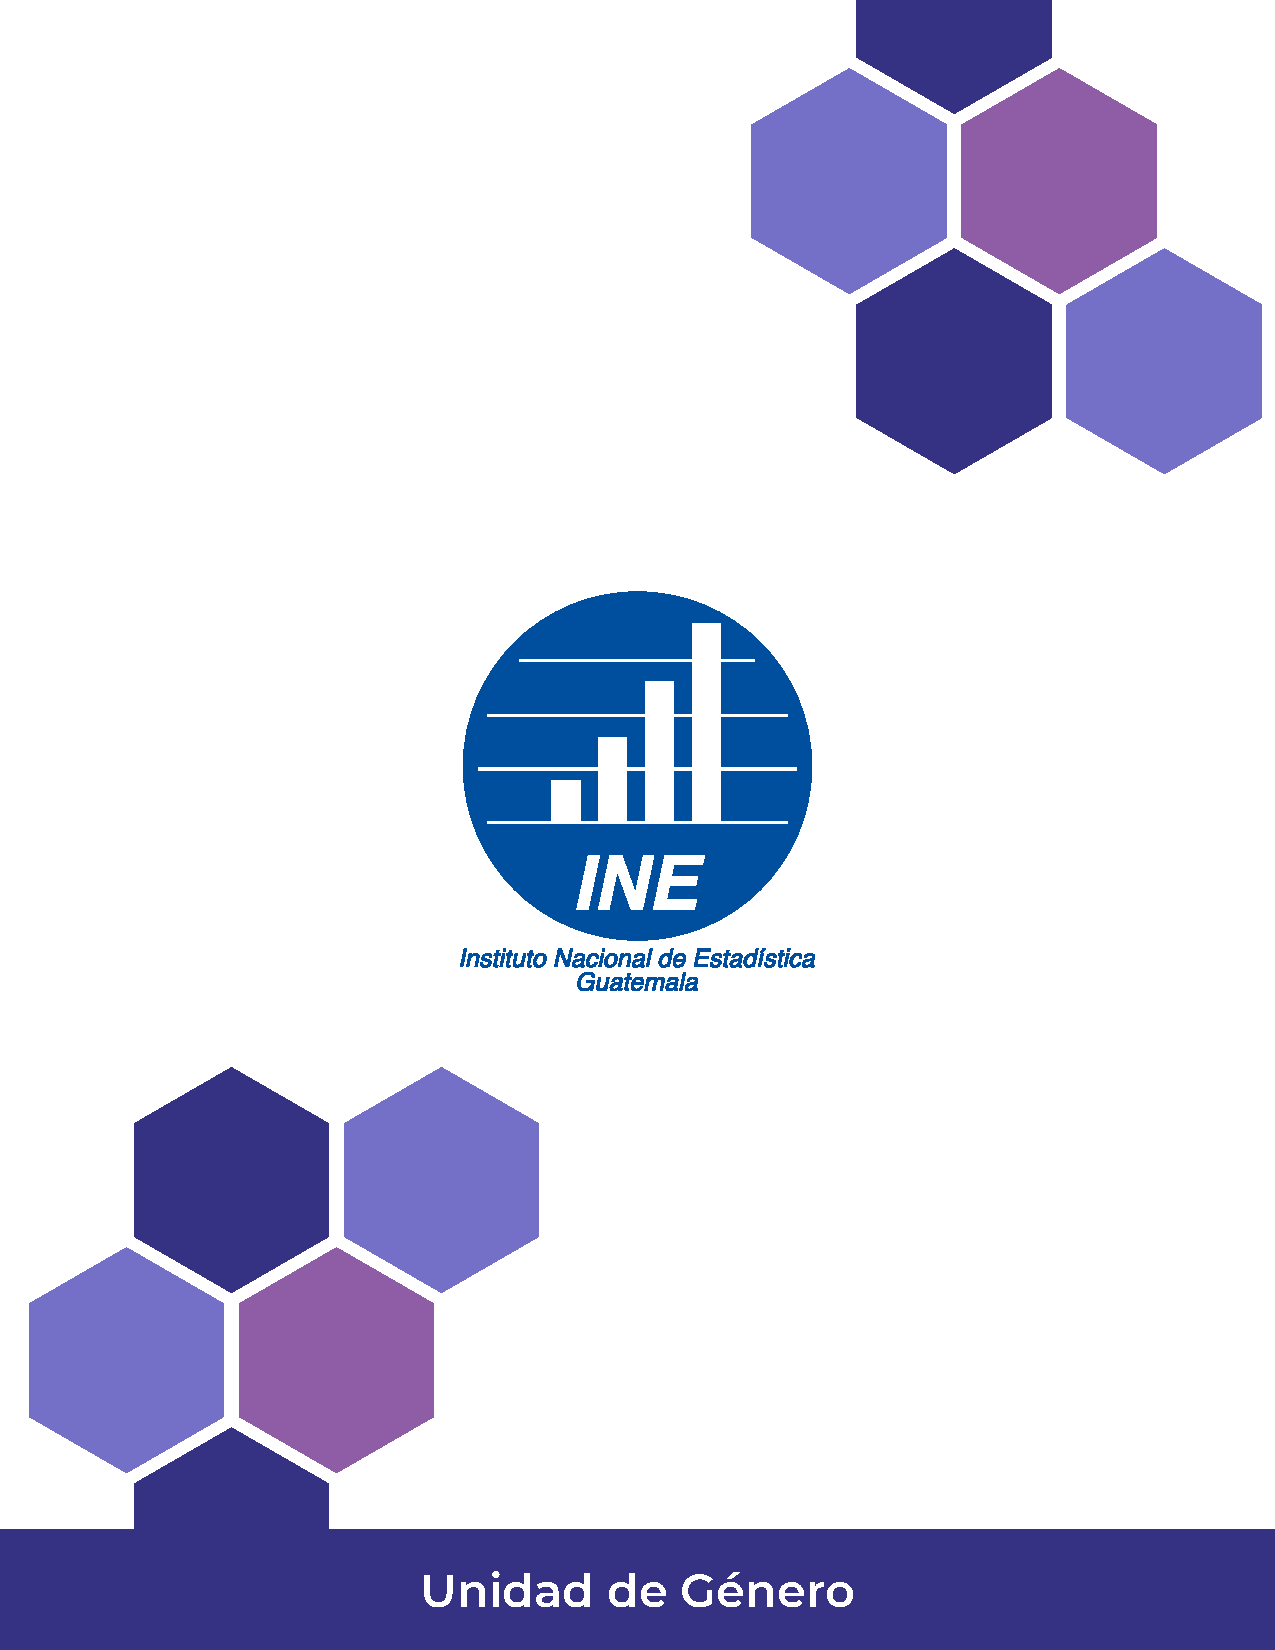
\includepdf{Plantilla/Contraportada_CEEG_2022.pdf}
	
	
\end{document}